\documentclass[12pt,a4paper]{article}

% ====== PACOTES ESSENCIAIS ======
\usepackage{lmodern}
\usepackage[utf8]{inputenc}
\usepackage[T1]{fontenc}
\usepackage[portuguese]{babel}
\usepackage{geometry}
\geometry{a4paper, top=2.5cm, bottom=2.5cm, left=3cm, right=2cm}
\usepackage{xcolor}
\usepackage{graphicx}
\usepackage{booktabs}
\usepackage{hyperref}
\usepackage{amsmath}
\usepackage{float} % Necessário para forçar a posição das imagens com [H]

% ====== CONFIGURAÇÃO DE LINKS ======
\hypersetup{
    colorlinks=true,
    linkcolor=blue,
    filecolor=magenta,      
    urlcolor=cyan,
    pdftitle={STM32 - Tutorial},
}

% ====== CONFIGURAÇÃO PARA BLOCOS DE CÓDIGO (C/C++) ======
\usepackage{listings}
\lstdefinestyle{CStyle}{
    language=C,
    backgroundcolor=\color{gray!5},   
    commentstyle=\color{green!60!black}\itshape,
    keywordstyle=\color{blue}\bfseries,
    numberstyle=\tiny\color{gray},
    stringstyle=\color{purple},
    basicstyle=\ttfamily\footnotesize,
    breakatwhitespace=false,         
    breaklines=true,                 
    captionpos=b,                    
    keepspaces=true,                 
    numbers=left,                    
    numbersep=5pt,                  
    showspaces=false,                
    showstringspaces=false,
    showtabs=false,                  
    tabsize=2,
    frame=single,
    rulecolor=\color{lightgray}
}
\lstset{style=CStyle}

% ====== CONFIGURAÇÃO PARA BLOCOS DE CÓDIGO (C/C++) ======
\usepackage{listings}
\lstdefinestyle{CStyle}{
    language=C,
    backgroundcolor=\color{gray!5},   
    commentstyle=\color{green!60!black}\itshape,
    keywordstyle=\color{blue}\bfseries,
    numberstyle=\tiny\color{gray},
    stringstyle=\color{purple},
    basicstyle=\ttfamily\footnotesize,
    breakatwhitespace=false,         
    breaklines=true,                 
    captionpos=b,                    
    keepspaces=true,                 
    numbers=left,                    
    numbersep=5pt,                  
    showspaces=false,                
    showstringspaces=false,
    showtabs=false,                  
    tabsize=2,
    frame=single,
    rulecolor=\color{lightgray},
    % === SOLUÇÃO DOS ACENTOS ===
    literate={~}{{$\sim$}}1
    {á}{{\'a}}1 {é}{{\'e}}1 {í}{{\'i}}1 {ó}{{\'o}}1 {ú}{{\'u}}1
             {Á}{{\'A}}1 {É}{{\'E}}1 {Í}{{\'I}}1 {Ó}{{\'O}}1 {Ú}{{\'U}}1
             {à}{{\`a}}1 {è}{{\`e}}1 {ì}{{\`i}}1 {ò}{{\`o}}1 {ù}{{\`u}}1
             {À}{{\`A}}1 {È}{{\'E}}1 {Ì}{{\`I}}1 {Ò}{{\`O}}1 {Ù}{{\`U}}1
             {ã}{{\~a}}1 {ẽ}{{\~e}}1 {ĩ}{{\~i}}1 {õ}{{\~o}}1 {ũ}{{\~u}}1
             {Ã}{{\~A}}1 {Ẽ}{{\~E}}1 {Ĩ}{{\~I}}1 {Õ}{{\~O}}1 {Ũ}{{\~U}}1
             {â}{{\^a}}1 {ê}{{\^e}}1 {î}{{\^i}}1 {ô}{{\^o}}1 {û}{{\^u}}1
             {Â}{{\^A}}1 {Ê}{{\^E}}1 {Î}{{\^I}}1 {Ô}{{\^O}}1 {Û}{{\^U}}1
             {ç}{{\c c}}1 {Ç}{{\c C}}1
}
\lstset{style=CStyle}

% ====== DADOS DO DOCUMENTO ======
\title{\textbf{STM32 - Tutorial}\\ \large Guia Prático e Implementações}
\author{Júnior Bandeira}
\date{Fevereiro de 2026}

\definecolor{pastelbg}{HTML}{FDF6E3} 
\pagecolor{pastelbg}

\begin{document}

% =====================================================================
% CAPA PERSONALIZADA HIGH-TECH
% =====================================================================
\begin{titlepage}
    \centering % Centraliza tudo na página

    % --- Título Principal ---
    \vspace*{1cm} % Espaço do topo
    {\Huge \textbf{Manual de Desenvolvimento STM32}}\\[0.5cm]
    
    % --- Subtítulo ---
    {\Large \textit{Do Bare-Metal e Registradores à Abstração da HAL}}\\[1.5cm]

    % --- A Imagem High-Tech ---
    % O comando abaixo busca a imagem que você salvou na pasta.
    % Ajuste 'width=0.9\textwidth' se quiser ela um pouco maior (1.0) ou menor (0.8).
    \includegraphics[width=0.9\textwidth]{imagens/cpu_gemini.png}\\[1.5cm]
    
    % --- Detalhes do Autor/Projeto ---
    % NÃO ESQUEÇA DE COLOCAR SEU NOME AQUI EMBAIXO:
    {\Large \textbf{Autor: Júnior Bandeira}}\\[0.5cm] 
    
    {\large Focando na família ARM Cortex-M4 (STM32F4xx)}\\[2cm]

    \vfill % Empurra a data para o final da página, no rodapé

    % --- Data ---
    {\large Versão 1.0 -- \today} % A data de hoje automática

\end{titlepage}
% A próxima página será o sumário, e o contador de páginas reinicia depois dela.
\clearpage
% =====================================================================

\thispagestyle{empty} % Tira o número da página da capa

\newpage % Pula para uma página limpa
\tableofcontents % GERA O SUMÁRIO AUTOMATICAMENTE AQUI
\newpage % Pula para outra página limpa para começar o texto

% ==========================================
% TÍTULO E LINKS ÚTEIS
% ==========================================
\begin{center}
    \Large\textbf{STM32 (Um Guia Nem Um Pouco Ortodoxo)}
\end{center}

\vspace{0.5cm}
\noindent\textbf{Links Úteis:}
\begin{itemize}
    \item \href{https://developer.arm.com/documentation/dui0553/latest/}{Cortex-M4 Devices Generic User Guide}
    \item \href{https://www.st.com/resource/ja/reference_manual/dm00119316-stm32f411xc-e-advanced-arm-based-32-bit-mcus-stmicroelectronics.pdf}{Reference Manual para o STM32F411}
    \item \href{https://www.st.com/resource/ja/user_manual/dm00105879-description-of-stm32f4-hal-and-ll-drivers-stmicroelectronics.pdf}{Description of STM32F4 HAL and LL drivers}
\end{itemize}



% ==========================================
% CARACTERÍSTICAS GERAIS
% ==========================================
\section*{Características Gerais}
\addcontentsline{toc}{section}{Características Gerais} % Adiciona ao sumário mesmo sem numeração

Os microcontroladores STM32 são baseados na arquitetura ARM Cortex-M (32-bits RISC). Diferenciam-se dos microcontroladores de 8 bits (como AVR/Arduino Uno) por:
\begin{itemize}
    \item \textbf{Arquitetura de Memória:} Geralmente Harvard (barramentos de instrução e dados separados) ou Harvard modificada, permitindo acesso simultâneo e maior velocidade.
    \item \textbf{Pipeline:} Execução de instruções em múltiplos estágios (fetch, decode, execute), aumentando o throughput.
    \item \textbf{Periféricos Complexos:} DMA (Acesso Direto à Memória), ADCs de alta velocidade (12-16 bits), Timers avançados e interfaces de comunicação dedicadas (SPI, I2C, UART, CAN, USB).
    \item \textbf{Interrupções:} Sistema NVIC (Nested Vectored Interrupt Controller) que gerencia prioridades e latência de interrupções de forma determinística.
\end{itemize}

% ==========================================
% SEÇÃO 1: TEORIA-BASE
% ==========================================
\section{Teoria-Base}

\subsection{Compilador e ST-Link}
\textbf{Compilador (Toolchain):} O padrão da indústria é o GCC (GNU Compiler Collection) na versão para ARM bare-metal, conhecido como \texttt{arm-none-eabi-gcc}.
\begin{itemize}
    \item \textbf{Processo:} Ocorre compilação cruzada (\textit{cross-compilation}). Você compila em uma arquitetura (x86/PC) para rodar em outra (ARM/MCU).
    \item \textbf{Saída:} O compilador gera arquivos binários (\texttt{.bin}, \texttt{.hex}) ou executáveis linkados (\texttt{.elf}) que contêm o código de máquina.
\end{itemize}

\textbf{ST-Link:} É o hardware de depuração e programação (\textit{debugger/programmer}).
\begin{itemize}
    \item \textbf{Função:} Atua como uma ponte entre o PC (USB) e o microcontrolador.
    \item \textbf{Protocolo:} Comunica-se com o chip via SWD (\textit{Serial Wire Debug}) – que usa apenas 2 pinos (Clock e IO) – ou JTAG (interface mais antiga e robusta, usa mais pinos).
    \item \textbf{Software:} No PC, ferramentas como OpenOCD ou ST-Link Server conversam com o hardware do ST-Link para gravar o firmware na memória Flash do MCU.
\end{itemize}

\subsection{CMSIS | LL | HAL}
Nível de Abstração: \textbf{HAL > LL > CMSIS}

\subsubsection{CMSIS (Common Microcontroller Software Interface Standard)}
Padrão definido pela ARM, é uma API, independente do fabricante do chip (ST, NXP, TI).
\begin{itemize}
    \item \textbf{O que é:} Define nomes padronizados para os registradores do núcleo (\textit{Core Peripherals} como NVIC, SysTick, MPU).
    \item \textbf{Vantagem:} Garante que o código de acesso ao núcleo do processador seja portável entre diferentes marcas que usam Cortex-M.
    \item \textbf{CMSIS-Device:} A ST fornece a extensão ``Device'', que mapeia os endereços de memória dos periféricos específicos (GPIO, ADC, SPI) para structs em C (ex: \texttt{GPIOA->ODR}). É o nível mais baixo de acesso em C.
\end{itemize}

\subsubsection{LL (Low Layer)}
Biblioteca proprietária da ST.
\begin{itemize}
    \item \textbf{Característica:} Uma camada fina acima dos registradores. As funções são basicamente inline que escrevem diretamente nos bits.
    \item \textbf{Prós:} Altíssima performance, tamanho de código reduzido (\textit{bloatware} quase zero).
    \item \textbf{Contras:} Não é totalmente portável entre famílias STM32 (ex: F1 para F4) se os registradores mudarem. Exige conhecimento profundo do \textit{datasheet}.
\end{itemize}

\subsubsection{HAL (Hardware Abstraction Level)}
Biblioteca de alto nível da ST.
\begin{itemize}
    \item \textbf{Característica:} Orientada a ``objetos'' (structs de configuração). Abstrai a complexidade do hardware.
    \item \textbf{Prós:} Portabilidade fácil entre famílias STM32, funções prontas para protocolos complexos (USB, Ethernet), acelera o desenvolvimento inicial.
    \item \textbf{Contras:} Lenta (muitas verificações de erro), consome muita Flash e RAM, esconde o funcionamento real do hardware.
\end{itemize}

\subsection{É possível não utilizar IDE?}
\subsubsection{Sim, como?}
É possível desenvolver usando apenas linha de comando (CLI) e editores de texto (VS Code, Vim, Neovim, Sublime).
\begin{itemize}
    \item \textbf{Editor:} Para escrever o código C/C++.
    \item \textbf{Build System:} Make ou CMake. Você cria um arquivo (\texttt{Makefile} ou \texttt{CMakeLists.txt}) que diz ao compilador quais arquivos compilar e quais flags usar (ex: \texttt{-mcpu=cortex-m4}).
    \item \textbf{Compilador:} Instalação manual do \texttt{arm-none-eabi-gcc}.
    \item \textbf{Gravador/Debugger:} Uso do OpenOCD ou ST-Link Utilities via terminal para enviar o binário compilado para o chip.
\end{itemize}

\subsection{IDEs (e como configurá-las)}

\subsubsection{STM32CubeMX}
\textbf{Função:} Ferramenta gráfica de configuração inicial. Não edita código, apenas gera.
\begin{itemize}
    \item \textbf{Pinout:} Define graficamente qual pino é GPIO, SPI, UART, etc.
    \item \textbf{Clock Configuration:} Árvore de clock visual para ajustar PLLs, divisores e multiplicadores de frequência.
    \item \textbf{Project Manager:} Gera o código base (``esqueleto'') para diversas IDEs (CubeIDE, Keil, IAR) ou Makefiles.
\end{itemize}

\subsubsection{STM32CubeIDE}
\textbf{Base:} Eclipse + CDT (C/C++ Development Tooling) + GCC + GDB.

\textbf{Estrutura de Pastas:}
\begin{itemize}
    \item \texttt{Core/Src}: Onde fica o \texttt{main.c}, \texttt{stm32f4xx\_it.c} (interrupções) e \texttt{msp.c} (inicialização de hardware de baixo nível).
    \item \texttt{Core/Inc}: Arquivos de cabeçalho (\texttt{.h}), incluindo \texttt{main.h}.
    \item \texttt{Drivers/STM32xx\_HAL\_Driver}: O código fonte da biblioteca HAL.
    \item \texttt{Drivers/CMSIS}: Definições dos registradores e do núcleo ARM.
\end{itemize}

Abaixo, a árvore completa de um projeto padrão gerado:

\begin{verbatim}
Seu_Projeto/
|-- Binaries/
|-- Includes/
|-- Core/
|   |-- Inc/
|   |   |-- main.h -> Cabecalho principal do projeto 
|   |   |-- stm32f4xx_hal_conf.h -> Config da biblioteca HAL 
|   |   \-- stm32f4xx_it.h -> Cabecalho das rotinas de interrupcao
|   |-- Src/
|   |   |-- main.c -> Codigo fonte principal 
|   |   |-- stm32f4xx_hal_msp.c -> Inicializacao de hardware (MSP)
|   |   |-- stm32f4xx_it.c -> Handlers gerados pelo CubeMX 
|   |   |-- syscalls.c -> Implementacao de chamadas de sistema 
|   |   |-- sysmem.c -> Gerenciamento de memoria (heap/malloc)
|   |   \-- system_stm32f4xx.c -> Configuracao critica inicial 
|   \-- Startup/
|       \-- startup_stm32f411ceux.s -> Vetores de interrupcao (Assembly)
|-- Drivers/
|   |-- CMSIS/ -> Definicoes base do nucleo ARM Cortex-M 
|   \-- STM32F4xx_HAL_Driver/ -> Codigo fonte da biblioteca HAL
|-- Debug/ -> Pasta do arquivo binario final (.elf, .bin, .hex) 
|-- Seu_Projeto.ioc -> Config visual do STM32CubeMX 
|-- Seu_Projeto Debug.launch -> Configs para gravar e debugar 
|-- STM32F411CEUX_FLASH.ld -> Linker script (Flash)
\-- STM32F411CEUX_RAM.ld -> Linker script secundario (RAM)
\end{verbatim}

\subsubsection{PlatformIO}
\begin{itemize}
    \item \textbf{O que é:} Uma extensão (geralmente usada no VS Code) que gerencia toolchains e bibliotecas.
    \item \textbf{Diferencial:} Arquivo \texttt{platformio.ini}. Nele você define a placa, o framework (Arduino, CMSIS, STM32Cube/HAL, Zephyr) e as bibliotecas externas. Ele baixa o compilador e as dependências automaticamente.
\end{itemize}

\subsection{Drivers para Sensores}
Para integrar sensores (ex: acelerômetros, displays, sensores de temperatura) profissionalmente, evita-se colocar código de hardware dentro da lógica do driver.
\begin{itemize}
    \item \textbf{Abstração de I/O:} O driver do sensor não deve saber se está rodando num STM32 ou num Arduino. Ele deve receber ponteiros de função para leitura e escrita (Read/Write).
\end{itemize}

\textbf{Estrutura Típica em C:}
\begin{lstlisting}[language=C]
typedef struct {
    // Ponteiros para funções de hardware (definidas pelo usuário no main)
    int8_t (*write_reg)(uint8_t reg_addr, uint8_t *data, uint16_t len);
    int8_t (*read_reg)(uint8_t reg_addr, uint8_t *data, uint16_t len);
    void (*delay_ms)(uint32_t ms);
} Sensor_IO_t;
\end{lstlisting}

\textbf{Implementação:} O desenvolvedor escreve as funções de I2C/SPI usando a HAL ou LL e as passa para a \texttt{struct} do driver na inicialização. Isso torna o driver do sensor portátil para qualquer microcontrolador.

% ==========================================
% SEÇÃO 2: PRÁTICA E IMPLEMENTAÇÕES
% ==========================================
\section{Prática e Implementações}

\subsection{Escovando bits}

\subsubsection{Comandos Básicos}
\textbf{Manipulando os bits dos Registradores}
\begin{itemize}
    \item \texttt{REG}: registrador (CMSIS te dá macros com os nomes de cada).
    \item \texttt{bit number}: CMSIS te dá macros para os bits que você quer manipular num registrador.
\end{itemize}

\textit{(\texttt{OBS}: necessita conhecimento de lógica e operadores bitwise, ver \hyperref[anexo:1]{Anexo 1} se necessitar estudar/rever.)}

\vspace{0.3cm}
\noindent\textbf{Setar um bit para 1 (set):}
\begin{lstlisting}[language=C]
REG |= bit number;  // (OR Operation)
\end{lstlisting}

Exemplo:
\begin{verbatim}
REG:         xxxxxxxxxxxxxBxx
bit:         xxxxxxxxxxxxx1xx
REG |= bit:  xxxxxxxxxxxxx1xx  
\end{verbatim}
Ou em C: \lstinline{REG |= (1 << 2);}

\begin{quote}
\textit{Observe que você também pode representar como \texttt{0b1} (binário), \texttt{0x1} (hexadecimal) e \texttt{01} (octal). A forma hexadecimal e decimal são as mais preferidas. Em se tratando de evitar problemas com o C, é recomendado avisar pro compilador que esse número é um unsigned long, ou seja, que ele é um número de 32 bits (no caso do Cortex-M4) $\rightarrow$ \texttt{1UL} ou \texttt{0x1UL}.}
\end{quote}

\noindent\textbf{Setar um bit para 0 (reset):}
\begin{lstlisting}[language=C]
REG &= ~(bit number);  // (AND NOT Operation)
\end{lstlisting}

Exemplo:
\begin{verbatim}
REG:            xxxxxxxBxxxxxxxx
bit:            xxxxxxx1xxxxxxxx
REG &= ~(bit):  xxxxxxx0xxxxxxxx 
\end{verbatim}
Ou em C: \lstinline{REG &= ~(1 << 8);}

\vspace{0.3cm}
\noindent\textbf{Toggle (alternar: 0 $\rightarrow$ 1 e 1 $\rightarrow$ 0) um bit:}
\begin{lstlisting}[language=C]
REG ^= bit number;  // (XOR Operation)
\end{lstlisting}

Exemplo:
\begin{verbatim}
REG:          xxx0xxxxxxxxxxxx
bit:          xxx1xxxxxxxxxxxx
REG ^= bit:   xxx1xxxxxxxxxxxx  
\end{verbatim}
Ou em C: \lstinline{REG ^= (1 << 12);}

\vspace{0.3cm}
\noindent\textbf{while() e volatile:}
Enquanto esse bit não for 0 repita \texttt{\{\}}.
\textit{\texttt{OBS}: \texttt{Tipo\_de\_Pino} vai ficar mais claro no próximo tópico, apenas entenda como um registrador qualquer.}

\begin{lstlisting}[language=C]
while((Tipo_de_Pino->REG & bit number) != 0){}
// Ou:
while(Tipo_de_Pino->REG & bit number){}
\end{lstlisting}

Exemplo Prático (ADC):
\begin{lstlisting}[language=C]
ADC1->CR |= ADC_CR_ADCAL;
// Ao fim da calibração, o bit de calibração do ADC1->CR volta a ser 0
while((ADC1->CR & ADC_CR_ADCAL) != 0){} // Caso não tenha concluído, permaneça no loop
\end{lstlisting}
\textit{Perceba que registradores do ADC1 (ponteiro de uma struct), como o \texttt{CR}, são do tipo \texttt{\_\_IO}, que é um alias para o tipo \texttt{volatile} em C (como discutido a posteriori).}

% ==========================================
% GPIO
% ==========================================
\subsection{GPIO (General-Purpose Input/Output)}

\textit{\texttt{OBS}: Antes de ver mais sobre a lib do HAL em si ou do CMSIS, é mais simples iniciar com conceitos mais conhecidos, como o GPIO.
\\\texttt{Nota}: Todas as funções/arquivos do HAL estão no diretório \texttt{Drivers/STM32F4xx\_HAL\_Driver}, entenda que uso ele como base.}

O objetivo dessa parte é apresentar a parte básica do GPIO. O CubeMX abstrai muitas configurações de acordo com o que marcamos na sua interface gráfica:

\begin{figure}[H]
    \centering
    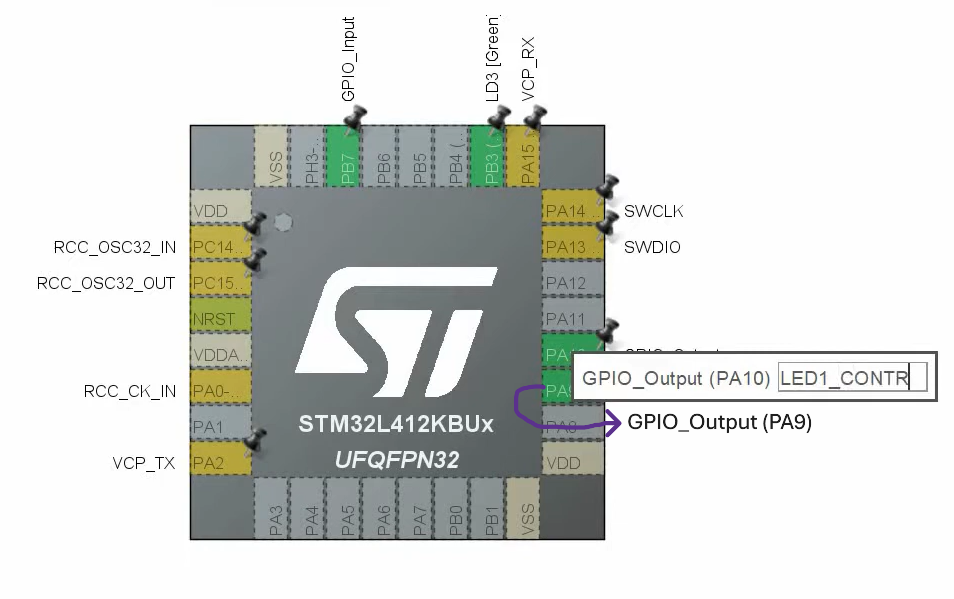
\includegraphics[width=0.8\linewidth]{imagens/Pinout_CubeMX.png}
    \caption{Pinout - CubeMX}
    \label{fig:pinout_cubemx}
\end{figure}

(Cada GPIO tem seus respectivos nome da porta e número do pino, como \texttt{GPIOA} e \texttt{GPIO\_PIN\_15} que é o pino 15 da porta A).

Por enquanto, esqueça os outros pinos que não são GPIO, temos os pinos 9 e 10 da porta A e os 3 e 7 da B. Perceba que se colocou labels neles para facilitar suas identificações, você pode fazer isso no código posteriormente. Agora, vamos fazer um LED acender com essas portas. Trabalharemos, em geral, com os arquivos da pasta \texttt{Core}. No \texttt{main.h} do seu subdiretório você vai encontrar os labels supramencionados e modificá-los ou adicioná-los, assim:

\begin{figure}[H]
    \centering
    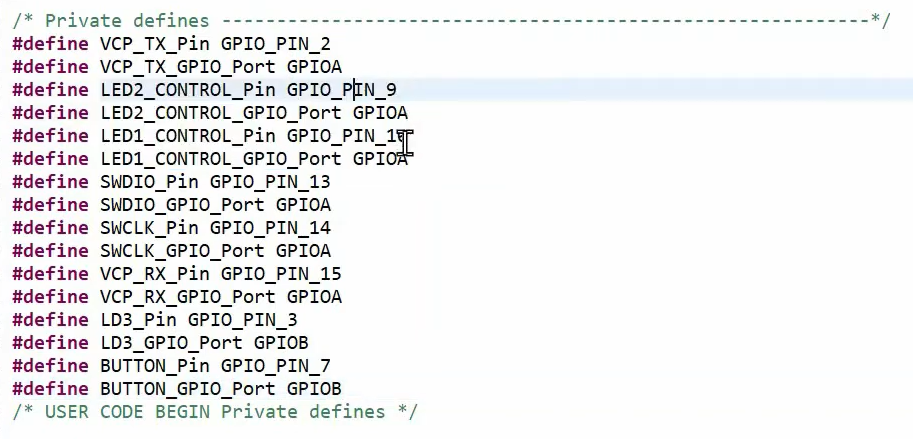
\includegraphics[width=0.8\linewidth]{imagens/Aliases.png}
    \caption{Aliases no arquivo de Header}
    \label{fig:aliases}
\end{figure}

Para identificar as macros e funções utilizadas pelo HAL para o GPIO, vá para o arquivo \texttt{Inc/stm32f4xx\_hal\_gpio.h} e \texttt{Src/stm32f4xx\_hal\_gpio.c}. O que precisamos agora é utilizar as funções de lá:

\begin{figure}[H]
    \centering
    \includegraphics[width=0.8\linewidth]{imagens/Hal_GPIO_Functions.png}
    \caption{Funções HAL GPIO}
    \label{fig:hal_gpio_func}
\end{figure}

Cabe, então, ter em mente dois desses tipos estranhos:

\begin{lstlisting}[language=C]
typedef enum
{
  GPIO_PIN_RESET = 0,
  GPIO_PIN_SET
} GPIO_PinState;
\end{lstlisting}

E o tipo que mapeia o hardware:
\begin{lstlisting}[language=C]
/**
 * @brief General Purpose I/O
 */
typedef struct
{
  __IO uint32_t MODER;    /*!< GPIO port mode register,               Address offset: 0x00      */
  __IO uint32_t OTYPER;   /*!< GPIO port output type register,        Address offset: 0x04      */
  __IO uint32_t OSPEEDR;  /*!< GPIO port output speed register,       Address offset: 0x08      */
  __IO uint32_t PUPDR;    /*!< GPIO port pull-up/pull-down register,  Address offset: 0x0C      */
  __IO uint32_t IDR;      /*!< GPIO port input data register,         Address offset: 0x10      */
  __IO uint32_t ODR;      /*!< GPIO port output data register,        Address offset: 0x14      */
  __IO uint32_t BSRR;     /*!< GPIO port bit set/reset register,      Address offset: 0x18      */
  __IO uint32_t LCKR;     /*!< GPIO port configuration lock register, Address offset: 0x1C      */
  __IO uint32_t AFR[2];   /*!< GPIO alternate function registers,     Address offset: 0x20-0x24 */
} GPIO_TypeDef;
\end{lstlisting}

\texttt{GPIO\_TypeDef} será especialmente importante para a parte sem HAL, visto que ele é uma struct do CMSIS. Falaremos melhor dele por lá.

Certo, agora, vejamos um exemplo da função que o CubeMX faz para utilizarmos, \texttt{MX\_GPIO\_Init()}:

\begin{lstlisting}[language=C]
static void MX_GPIO_Init(void)
{
  GPIO_InitTypeDef GPIO_InitStruct = {0};
  /* GPIO Ports Clock Enable */
  __HAL_RCC_GPIOC_CLK_ENABLE();
  __HAL_RCC_GPIOH_CLK_ENABLE();
  __HAL_RCC_GPIOA_CLK_ENABLE();
  __HAL_RCC_GPIOB_CLK_ENABLE();
  
  /*Configure GPIO pin Output Level */
  HAL_GPIO_WritePin(GPIOC, GPIO_PIN_13, GPIO_PIN_RESET);
  HAL_GPIO_WritePin(GPIOA, W25Q_CS_Pin|GPIO_PIN_15, GPIO_PIN_RESET);
  
  /*Configure GPIO pin : PC13 */
  GPIO_InitStruct.Pin = GPIO_PIN_13;
  GPIO_InitStruct.Mode = GPIO_MODE_OUTPUT_PP;
  GPIO_InitStruct.Pull = GPIO_NOPULL;
  GPIO_InitStruct.Speed = GPIO_SPEED_FREQ_LOW;
  HAL_GPIO_Init(GPIOC, &GPIO_InitStruct);
  
  // ... (outras configuracoes omitidas por brevidade) ...
}
\end{lstlisting}
Essa função é onde ficam as configurações de cada pino/porta GPIO que utilizaremos. Perceba que ele automaticamente utilizou o HAL. Partimos, pois, para ele. O exemplo usa um botão para acender dois LEDs.

\subsubsection{Com HAL}
A abstração cuida dos offsets de memória e oferece funções prontas para leitura/escrita. Primeiro, utilizaremos labels para ficar mais fácil a identificação de pinos e portas:

\begin{lstlisting}[language=C]
/* main.h */
#define B1_Pin GPIO_PIN_13        // Botao (PC13)
#define B1_GPIO_Port GPIOC

#define LD1_Pin GPIO_PIN_5        // LED 1 (PA5)
#define LD1_GPIO_Port GPIOA

#define LD2_Pin GPIO_PIN_6        // LED 2 (PA6)
#define LD2_GPIO_Port GPIOA
\end{lstlisting}

Lembrando a definição de uma porta \texttt{GPIOx} (definida pelo CMSIS), como exemplo a \texttt{GPIOA}:
\begin{lstlisting}[language=C]
#define GPIOA               ((GPIO_TypeDef *) GPIOA_BASE)
// Que e, por sua vez:
#define GPIOA_BASE          (AHB1PERIPH_BASE + 0x0000UL)
\end{lstlisting}
Portanto, \texttt{GPIOA\_BASE} é um endereço da memória que começa a porta A, e o \texttt{GPIOA} é um ponteiro que aponta para um \texttt{GPIO\_TypeDef} instanciado nesse endereço. Não se apegue às minúcias, o importante é que \texttt{GPIOx} é um ponteiro para uma struct.

\begin{lstlisting}[language=C]
/* main.c */
static void MX_GPIO_Init(void)
{
  GPIO_InitTypeDef GPIO_InitStruct = {0}; 
  /* 1. Habilita Clocks (veremos na parte de Clock) */
  __HAL_RCC_GPIOC_CLK_ENABLE();
  __HAL_RCC_GPIOA_CLK_ENABLE();

  /* 2. Configura LEDs (PA5 e PA6) como Saida */
  HAL_GPIO_WritePin(GPIOA, LD1_Pin|LD2_Pin, GPIO_PIN_RESET); // Inicia desligado (prevencao)

  GPIO_InitStruct.Pin = LD1_Pin|LD2_Pin; // Multiplos pinos com OR
  GPIO_InitStruct.Mode = GPIO_MODE_OUTPUT_PP; // Push-Pull
  GPIO_InitStruct.Pull = GPIO_NOPULL; // No pull
  GPIO_InitStruct.Speed = GPIO_SPEED_FREQ_LOW; // Evitar ruidos
  HAL_GPIO_Init(GPIOA, &GPIO_InitStruct); 

  /* 3. Configura Botao (PC13) como Entrada */
  GPIO_InitStruct.Pin = B1_Pin;
  GPIO_InitStruct.Mode = GPIO_MODE_INPUT;
  GPIO_InitStruct.Pull = GPIO_PULLUP; // Assumindo pull-up para botao desativado
  HAL_GPIO_Init(GPIOC, &GPIO_InitStruct);
}

/* Loop Principal (no main()) */
while (1)
{
  /* Leitura do Botao: Se pressionado (Baixo), acende LED 1 */
  if (HAL_GPIO_ReadPin(B1_GPIO_Port, B1_Pin) == GPIO_PIN_RESET)
  {
    HAL_GPIO_WritePin(LD1_GPIO_Port, LD1_Pin, GPIO_PIN_SET);
  }
  else
  {
    HAL_GPIO_WritePin(LD1_GPIO_Port, LD1_Pin, GPIO_PIN_RESET);
  }

  /* Pisca LED 2 independentemente do botao */
  HAL_GPIO_TogglePin(LD2_GPIO_Port, LD2_Pin);
  
  HAL_Delay(100); // Delay de 100ms
}
\end{lstlisting}

\textit{\texttt{OBS}: Para saber mais sobre os atributos Mode e Pull, veja o \hyperref[anexo:3]{Anexo 3}.} E é basicamente isso, utilizando o HAL. Vamos para a parte mais difícil.

\subsubsection{Com LL}

Acesso direto. Assume-se arquitetura padrão Cortex-M4 (STM32F4/L4), onde se usa \texttt{MODER} para modo e \texttt{BSRR} para escrita atômica. Ok, aqui as coisas ficam mais complicadas, vamos dar uma olhada na documentação para o \href{https://www.st.com/resource/ja/reference_manual/dm00119316-stm32f411xc-e-advanced-arm-based-32-bit-mcus-stmicroelectronics.pdf}{GPIO}, da página 158 em diante e entender como modificar cada registrador. Vale ressaltar a importância de ter entendido a parte anterior chamada: ``Escovando Bits''. 

Primeiro, lembre-se da definição de \texttt{GPIO\_TypeDef}:

\begin{lstlisting}[language=C]
typedef struct
{
  __IO uint32_t MODER;    /*!< GPIO port mode register,               Address offset: 0x00      */
  __IO uint32_t OTYPER;   /*!< GPIO port output type register,        Address offset: 0x04      */
  __IO uint32_t OSPEEDR;  /*!< GPIO port output speed register,       Address offset: 0x08      */
  __IO uint32_t PUPDR;    /*!< GPIO port pull-up/pull-down register,  Address offset: 0x0C      */
  __IO uint32_t IDR;      /*!< GPIO port input data register,         Address offset: 0x10      */
  __IO uint32_t ODR;      /*!< GPIO port output data register,        Address offset: 0x14      */
  __IO uint32_t BSRR;     /*!< GPIO port bit set/reset register,      Address offset: 0x18      */
  __IO uint32_t LCKR;     /*!< GPIO port configuration lock register, Address offset: 0x1C      */
  __IO uint32_t AFR[2];   /*!< GPIO alternate function registers,     Address offset: 0x20-0x24 */
} GPIO_TypeDef;
\end{lstlisting}

Beleza, entenda que cada um desses \texttt{\_\_IO uint32\_t} são registradores 32-bit, escrever neles que vai definir como nosso pino de uma porta \texttt{GPIOx} vai funcionar. Mas o que é o \texttt{\_\_IO}? ``\texttt{\_\_IO}'' é um apelido do CMSIS para o qualificador ``volatile'' em C, esse modificador de tipo: \textit{``informa ao compilador que o valor de uma variável pode mudar a qualquer momento por agentes externos (hardware, interrupções ou threads), impedindo otimizações que a manteriam em um registrador. Ele garante que cada leitura/escrita acesse a memória física, sendo essencial para sistemas embarcados e multithreading''.}

Maneiro, agora a gente ``só'' precisa entender como atribuir os inteiros corretos a esses registradores para conseguirmos definir nossos pinos. Vamos lá, eu vou apresentar o código aos poucos e te mostrar a documentação. Primeiro, começaremos com uma versão sem ter as partes de pull, speed e mode push-pull/open-drain, será uma versão mais tranquila para entender aos poucos, ao fim adicionaremos tudo isso. 

Comecemos definindo o valor para o registrador \texttt{AHB1ENR}, esse vai ser explicado na parte de clock. Vamos criar nossa própria função \texttt{gpioInitDirect()}:

\begin{lstlisting}[language=C]
/* main.c */
static void gpioInitDirect(void)
{
  /* 1. Habilita Clocks (AHB1) para Portas A e C */
  // Bit 0 = GPIOA, Bit 2 = GPIOC
  RCC->AHB1ENR |= (1UL << 0) | (1UL << 2);
\end{lstlisting}

Olhando agora para o registrador \texttt{MODER}, perceba que queremos modificar os bits dos \texttt{MODER5} e \texttt{MODER6} da nossa porta A, ou seja, setar o tipo de modo dos pinos 5 e 6 de A:

\begin{figure}[H]
    \centering
    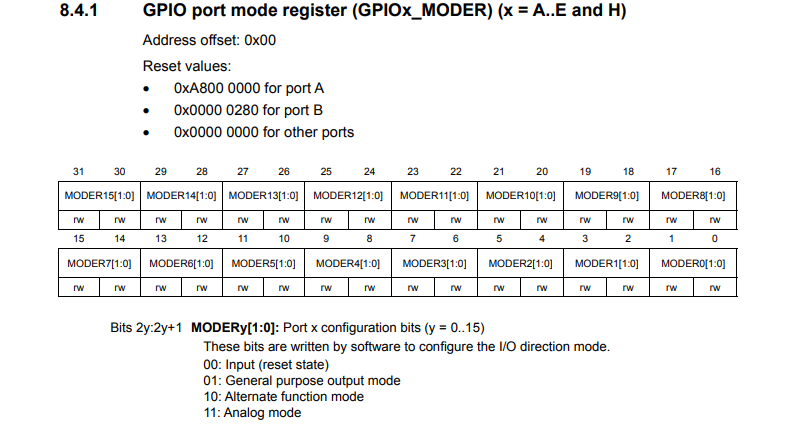
\includegraphics[width=0.8\linewidth]{imagens/GPIOx_MODER.png}
    \caption{GPIOx\_MODER}
    \label{fig:gpiox_moder}
\end{figure}

Nesse caso, queremos que os dois sejam outputs, ou seja: \texttt{0b01} ou \texttt{0x01}. E os endereços de \texttt{MODER5} e \texttt{MODER6} no offset desse registrador são, respectivamente, nos bits [10 e 11] e [12 e 13] (perceba que seus endereços iniciais são o dobro do número do pino). Vamos para o código:

\begin{lstlisting}[language=C]
  /* 2. Configura LEDs (PA5 e PA6) como Saida (01) */
  // Limpa os bits referentes aos pinos 5 e 6
  GPIOA->MODER &= ~((0x3UL << (5 * 2)) | (0x3UL << (6 * 2))); 
  // UL e para deixar claro que sao unsigned longs, ou seja, nesse caso, 32 bits
  // Seta para 01 (Output)
  GPIOA->MODER |=  ((0x1UL << (5 * 2)) | (0x1UL << (6 * 2)));

  /* 3. Configura Botao (PC13) como Entrada (00) */
  // Limpa os bits do pino 13 (Reset state ja e 00, mas por seguranca:)
  GPIOC->MODER &= ~(0x3UL << (13 * 2));
}
\end{lstlisting}

Claro, isso está muito cru, precisamos usar aliases para facilitar leitura e modificações, faremos isso depois do loop. O loop precisa, então, modificar o valor de saída ou entrada dos pinos, para isso, precisamos definir os valores dos registradores \texttt{IDR} (leitura), \texttt{ODR} (escrita) e \texttt{BSRR} (escrita) das portas. Vejamos:

\begin{figure}[H]
    \centering
    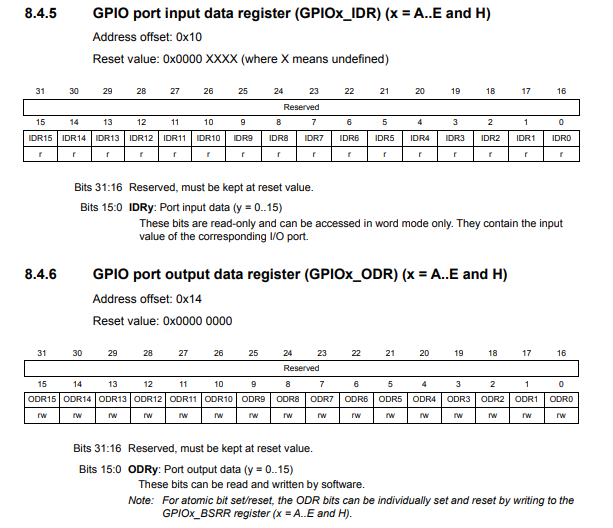
\includegraphics[width=0.8\linewidth]{imagens/GPIOx_IDR_ODR.png}
    \caption{GPIOx\_IDR e GPIOx\_ODR}
    \label{fig:gpiox_idr_odr}
\end{figure}

Perceba que esses registradores tem apenas 16 bits modificáveis. Precisamos ativar o bit 13 para ler o valor de input do pino 13 do botão. Já para os LEDs, setar (colocar 1) no pino 5 e 6 para acender e resetar (colocar 0) para apagar. Mas precisamos de outro registrador chamado \texttt{BSRR}, que seta e reseta o valor do pino de output, ou seja, ele modifica o \texttt{ODR} indiretamente:

\begin{figure}[H]
    \centering
    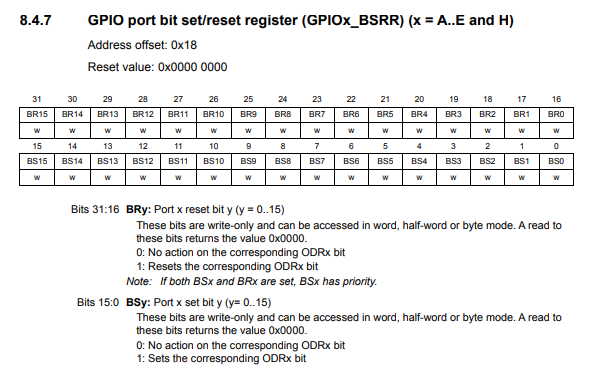
\includegraphics[width=0.8\linewidth]{imagens/GPIOx_BSRR.png}
    \caption{GPIOx\_BSRR}
    \label{fig:gpiox_bsrr}
\end{figure}

Então, utilizaremos os dois registradores para fins de prática nos LEDs. Vamos para o código:

\begin{lstlisting}[language=C]
/* Loop Principal (no main())*/
// Lembrando que voce tem que chamar o gpioInitDirect() no main() antes

while (1)
{
  /* Leitura: Checa o Bit 13 do Registrador de Entrada (IDR) */
  if (GPIOC->IDR & (0x1UL << 13)) 
  {
    /* Escreve 1 no Bit 5 do BSRR (Set) -> Liga LED 1 */
    GPIOA->BSRR = (0x1UL << 5); 
  }
  else
  {
    /* Escreve 1 no Bit 21 (5 + 16) do BSRR (Reset) -> Desliga LED 1 */
    GPIOA->BSRR = (0x1UL << (5 + 16)); 
  }

  /* Toggle LED 2: XOR no Registrador de Saida (ODR) bit 6 */
  GPIOA->ODR ^= (0x1UL << 6); // Isso e um toggle simples com ODR, mas nao e seguro como o BSRR

  /* Delay rustico (ja que nao temos HAL_Delay configurado aqui) */
  for (volatile int i = 0; i < 100000; i++);
}
\end{lstlisting}

``Porquê usar o BSSR e não o ODR?''... você pode se perguntar, tem a ver com a parte de Interrupts (mais para frente) e atomicidade, mas a justificativa está no \hyperref[anexo:4]{Anexo 4}, se tiver ansioso.

Ok, agora vamos ajustar algumas coisas, definiremos certas macros para facilitar escrita e mudança no \texttt{main.h} e adicionaremos as partes de pull/speed/mode push-pull/open-drain; para resumir, irei apenas mostrar nossas macros e não entrarei em detalhes desses outros registradores, visto que agora você deve ser capaz de entender por conta própria pela documentação a seguir. Os macros:

\begin{figure}[H]
    \centering
    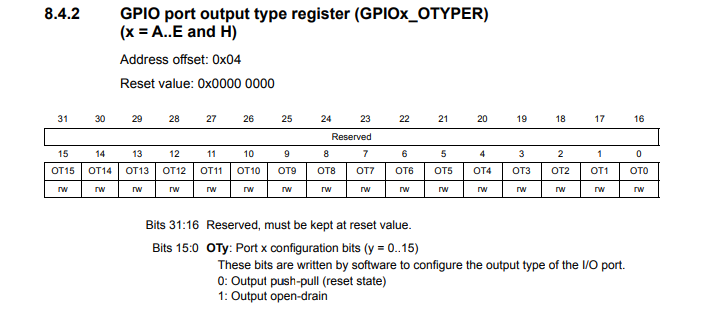
\includegraphics[width=0.8\linewidth]{imagens/GPIOx_OTYPER.png}
    \caption{GPIOx\_OTYPER}
    \label{fig:gpiox_otyper}
\end{figure}

\begin{figure}[H]
    \centering
    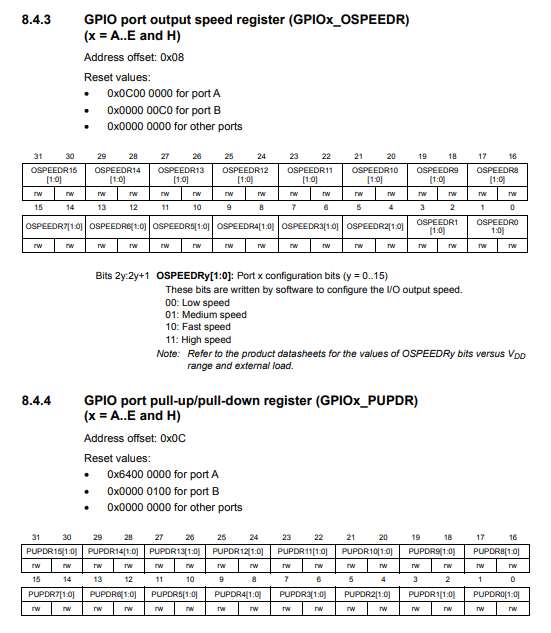
\includegraphics[width=0.8\linewidth]{imagens/GPIOx_OSPEEDR_PUPDR.png}
    \caption{GPIOx\_OSPEEDR e GPIOx\_PUPDR}
    \label{fig:gpiox_ospeedr_pupdr}
\end{figure}

\begin{lstlisting}[language=C]
/* main.h */
#include <stdint.h> // lembra de estar incluindo

/* --- Definicoes de Hardware --- */
// Botao (PC13)
#define B1_PIN        13
#define B1_PORT       GPIOC

// LED 1 (PA5)
#define LD1_PIN       5
#define LD1_PORT      GPIOA

// LED 2 (PA6)
#define LD2_PIN       6
#define LD2_PORT      GPIOA

/* --- Constantes de Configuracao (Baseado no Reference Manual) --- */
// MODER (2 bits)
#define GPIO_MODE_INPUT     0x00UL
#define GPIO_MODE_OUTPUT    0x01UL
#define GPIO_MODE_AF        0x02UL
#define GPIO_MODE_ANALOG    0x03UL

// OTYPER (1 bit)
#define GPIO_TYPE_PP        0x00UL // Push-Pull
#define GPIO_TYPE_OD        0x01UL // Open-Drain

// OSPEEDR (2 bits)
#define GPIO_SPEED_LOW      0x00UL
#define GPIO_SPEED_MEDIUM   0x01UL
#define GPIO_SPEED_FAST     0x02UL
#define GPIO_SPEED_HIGH     0x03UL

// PUPDR (2 bits)
#define GPIO_NOPULL         0x00UL
#define GPIO_PULLUP         0x01UL
#define GPIO_PULLDOWN       0x02UL

/* --- MACROS INTELIGENTES DE FUNCAO --- */
// Nosso mini HAL

// Configura registradores de 2 bits (MODER, PUPDR, OSPEEDR)
// Logica: Limpa os 2 bits na posicao (PIN*2) e escreve o novo valor
#define GPIO_CONFIG_2BIT(PORT, PIN, REG, VALUE) \
    (PORT)->REG = ((PORT)->REG & ~(0x3UL << ((PIN) * 2))) | ((VALUE) << ((PIN) * 2))

// Configura registradores de 1 bit (OTYPER)
#define GPIO_CONFIG_1BIT(PORT, PIN, REG, VALUE) \
    (PORT)->REG = ((PORT)->REG & ~(0x1UL << (PIN))) | ((VALUE) << (PIN))

// Macros de Operacao (Leitura/Escrita)
#define GPIO_WRITE_HIGH(PORT, PIN)   ((PORT)->BSRR = (0x1UL << (PIN)))
#define GPIO_WRITE_LOW(PORT, PIN)    ((PORT)->BSRR = (0x1UL << ((PIN) + 16)))
#define GPIO_TOGGLE(PORT, PIN)       ((PORT)->ODR  ^= (0x1UL << (PIN)))
#define GPIO_READ(PORT, PIN)         (((PORT)->IDR >> (PIN)) & 0x1UL)
\end{lstlisting}

Vou dar duas versões, uma sem e outra com as macros de funções. A sem, mais crua:

\begin{lstlisting}[language=C]
/* main.c */
#include "main.h"

static void gpioInitDirect(void)
{
  /* 1. Habilita Clocks (AHB1) */
  RCC->AHB1ENR |= (RCC_AHB1ENR_GPIOAEN | RCC_AHB1ENR_GPIOCEN);

  GPIOA->BSRR = (0x1UL << (LD1_PIN + 16)) | (0x1UL << (LD2_PIN + 16)); // Reseta os LEDs (prevencao)

  /* ========================================================== */
  /* CONFIGURACAO DO LED 1 (PA5) - Output, Push-Pull, Low Speed */
  /* ========================================================== */
  
  /* A. MODER (2 bits): Configura como OUTPUT (01) */
  GPIOA->MODER &= ~(0x3UL << (LD1_PIN * 2));          // Limpa (zera os 2 bits)
  GPIOA->MODER |=  (GPIO_MODE_OUTPUT << (LD1_PIN * 2)); // Escreve 01

  /* B. OTYPER (1 bit): Configura como Push-Pull (0) */
  GPIOA->OTYPER &= ~(0x1UL << LD1_PIN);               // Limpa (bit vira 0 = PP)
  // Nota: Se fosse Open-Drain, fariamos: |= (GPIO_TYPE_OD << LD1_PIN);

  /* C. OSPEEDR (2 bits): Configura como Low Speed (00) */
  GPIOA->OSPEEDR &= ~(0x3UL << (LD1_PIN * 2));        // Limpa (00 = Low)
  GPIOA->OSPEEDR |=  (GPIO_SPEED_LOW << (LD1_PIN * 2));

  /* D. PUPDR (2 bits): Configura como No Pull (00) */
  GPIOA->PUPDR &= ~(0x3UL << (LD1_PIN * 2));          // Limpa (00 = No Pull)
  GPIOA->PUPDR |=  (GPIO_NOPULL << (LD1_PIN * 2));


  /* ========================================================== */
  /* CONFIGURACAO DO LED 2 (PA6) - Output, Push-Pull, Low Speed */
  /* ========================================================== */
  
  /* A. MODER */
  GPIOA->MODER &= ~(0x3UL << (LD2_PIN * 2));
  GPIOA->MODER |=  (GPIO_MODE_OUTPUT << (LD2_PIN * 2));

  /* B. OTYPER */
  GPIOA->OTYPER &= ~(0x1UL << LD2_PIN);

  /* C. OSPEEDR */
  GPIOA->OSPEEDR &= ~(0x3UL << (LD2_PIN * 2));
  GPIOA->OSPEEDR |=  (GPIO_SPEED_LOW << (LD2_PIN * 2));

  /* D. PUPDR */
  GPIOA->PUPDR &= ~(0x3UL << (LD2_PIN * 2));
  GPIOA->PUPDR |=  (GPIO_NOPULL << (LD2_PIN * 2));

/* Se voce quiser economizar a mao, podemos encurtar a config dos LEDs: */

  /* A. MODER (2 bits/pino): Limpa os bits de ambos e seta como OUTPUT (01) */
  GPIOA->MODER &= ~((0x3UL << (LD1_PIN * 2)) | (0x3UL << (LD2_PIN * 2)));
  GPIOA->MODER |=  ((GPIO_MODE_OUTPUT << (LD1_PIN * 2)) | (GPIO_MODE_OUTPUT << (LD2_PIN * 2)));

  /* B. OTYPER (1 bit/pino): Limpa os bits de ambos (0 = Push-Pull) */
  GPIOA->OTYPER &= ~((0x1UL << LD1_PIN) | (0x1UL << LD2_PIN));
  /* Se fosse Open-Drain, fariamos: |= ((GPIO_TYPE_OD << LD1_PIN) | (GPIO_TYPE_OD << LD2_PIN)); */

  /* C. OSPEEDR (2 bits/pino): Limpa os bits de ambos (00 = Low Speed) */
  GPIOA->OSPEEDR &= ~((0x3UL << (LD1_PIN * 2)) | (0x3UL << (LD2_PIN * 2)));
  /* Omitido o passo |= pois GPIO_SPEED_LOW ja e 0x00UL */

  /* D. PUPDR (2 bits/pino): Limpa os bits de ambos (00 = No Pull) */
  GPIOA->PUPDR &= ~((0x3UL << (LD1_PIN * 2)) | (0x3UL << (LD2_PIN * 2)));
  /* Omitido o passo |= pois GPIO_NOPULL ja e 0x00UL */


  /* ========================================================== */
  /* CONFIGURACAO DO BOTAO (PC13) - Input, No Pull            */
  /* ========================================================== */
  
  /* A. MODER: Configura como INPUT (00) */
  GPIOC->MODER &= ~(0x3UL << (B1_PIN * 2));           // Limpa (00 = Input)
  GPIOC->MODER |=  (GPIO_MODE_INPUT << (B1_PIN * 2));

  /* B. PUPDR: Configura como No Pull (00) */
  GPIOC->PUPDR &= ~(0x3UL << (B1_PIN * 2));
  GPIOC->PUPDR |=  (GPIO_PULLUP << (B1_PIN * 2));
  
  /* Nota: OTYPER e OSPEEDR sao ignorados quando o pino e Input */  
}

int main(void)
{
  gpioInitDirect();

  while (1)
  {
    /* LEITURA: IDR (Input Data Register) */
    /* Verifica se o bit do botao esta em nivel BAIXO (0) */
    if (!(GPIOC->IDR & (1UL << B1_PIN))) 
    {
      /* ESCRITA (Ligar): BSRR (Bit Set/Reset Register) */
      /* Escreve 1 na metade INFERIOR do registrador (Bits 0-15) para SETAR */
      GPIOA->BSRR = (1UL << LD1_PIN);
    }
    else
    {
      /* ESCRITA (Desligar): BSRR */
      /* Escreve 1 na metade SUPERIOR do registrador (Bits 16-31) para RESETAR */
      GPIOA->BSRR = (1UL << (LD1_PIN + 16));
    }

    /* TOGGLE: ODR (Output Data Register) */
    /* Usa XOR para inverter apenas o bit do LED 2 */
    GPIOA->ODR ^= (1UL << LD2_PIN);

    /* Delay */
    for (volatile int i = 0; i < 100000; i++);
  }
}
\end{lstlisting}

A com os macros, mais parecida com o HAL:

\begin{lstlisting}[language=C]
/* main.c */
#include "main.h"

static void gpioInitDirect(void)
{
  /* 1. Habilita Clocks (AHB1) */
  RCC->AHB1ENR |= (RCC_AHB1ENR_GPIOAEN | RCC_AHB1ENR_GPIOCEN);

  GPIO_WRITE_LOW(LD1_PORT, LD1_PIN); // Reseta os LEDs (prevencao)
  GPIO_WRITE_LOW(LD2_PORT, LD2_PIN);

  /* --- Configuracao do LED 1 (PA5) --- */
  // Equivalente HAL: Mode=Output_PP, Pull=NoPull, Speed=Low
  GPIO_CONFIG_2BIT(LD1_PORT, LD1_PIN, MODER,   GPIO_MODE_OUTPUT); // Mode
  GPIO_CONFIG_1BIT(LD1_PORT, LD1_PIN, OTYPER,  GPIO_TYPE_PP);     // Type
  GPIO_CONFIG_2BIT(LD1_PORT, LD1_PIN, OSPEEDR, GPIO_SPEED_LOW);   // Speed
  GPIO_CONFIG_2BIT(LD1_PORT, LD1_PIN, PUPDR,   GPIO_NOPULL);      // Pull

  /* --- Configuracao do LED 2 (PA6) --- */
  // Equivalente HAL: Mode=Output_PP, Pull=NoPull, Speed=Low
  GPIO_CONFIG_2BIT(LD2_PORT, LD2_PIN, MODER,   GPIO_MODE_OUTPUT);
  GPIO_CONFIG_1BIT(LD2_PORT, LD2_PIN, OTYPER,  GPIO_TYPE_PP);
  GPIO_CONFIG_2BIT(LD2_PORT, LD2_PIN, OSPEEDR, GPIO_SPEED_LOW);
  GPIO_CONFIG_2BIT(LD2_PORT, LD2_PIN, PUPDR,   GPIO_NOPULL);

  /* --- Configuracao do Botao (PC13) --- */
  // Equivalente HAL: Mode=Input, Pull=NoPull (ou PullUp dependendo da placa)
  GPIO_CONFIG_2BIT(B1_PORT, B1_PIN, MODER,   GPIO_MODE_INPUT);
  GPIO_CONFIG_2BIT(B1_PORT, B1_PIN, PUPDR,   GPIO_PULLUP); 
  // Nota: OTYPER e OSPEEDR nao afetam pinos em modo INPUT
}

int main(void)
{
  /* Inicializa o hardware */
  gpioInitDirect();

  while (1)
  {
    /* Leitura: Se botao PC13 estiver LOW (0) */
    if (!GPIO_READ(B1_PORT, B1_PIN)) 
    {
      /* Liga LED 1 */
      GPIO_WRITE_HIGH(LD1_PORT, LD1_PIN);
    }
    else
    {
      /* Desliga LED 1 */
      GPIO_WRITE_LOW(LD1_PORT, LD1_PIN);
    }

    /* Toggle LED 2 */
    GPIO_TOGGLE(LD2_PORT, LD2_PIN);

    /* Delay rustico */
    for (volatile int i = 0; i < 100000; i++);
  }
}
\end{lstlisting}

Uff, punk, acabou, então, a parte de GPIO. Mas se você conseguiu entender até aqui, o resto deve ser mais suave. Os próximos códigos feitos com LL (Bare-Metal) não ficarão usando aliases/apelidos que demos nos headers, então só saiba que você pode definí-los à vontade.


% ==========================================
% INTERRUPTS
% ==========================================
\subsection{Interrupts}

\begin{figure}[H]
    \centering
    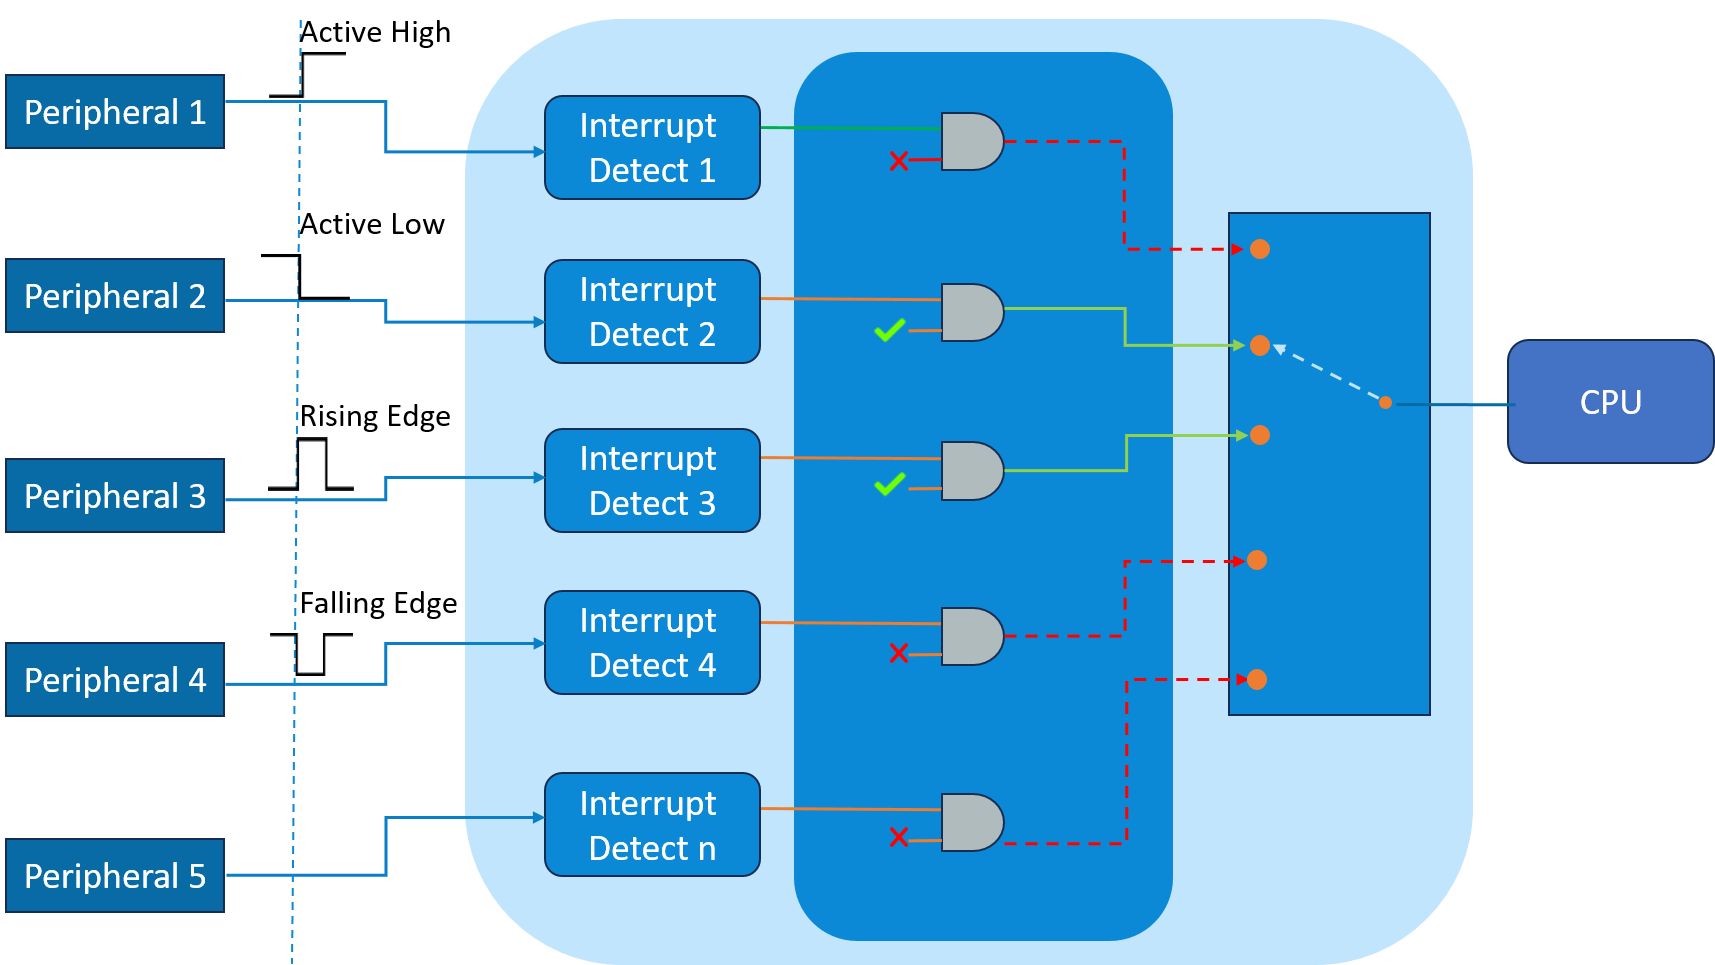
\includegraphics[width=0.8\linewidth]{imagens/Interrupts.png}
    \caption{Interrupts}
    \label{fig:interrupts}
\end{figure}

Em sistemas embarcados, existem duas formas de verificar se um evento ocorreu (como apertar um botão):
\begin{itemize}
    \item \textbf{Polling (Pesquisa):} O processador fica constantemente perguntando no \texttt{while(1)}: ``O botão foi apertado? O botão foi apertado?''. Isso desperdiça ciclos de processamento e energia.
    \item \textbf{Interrupt (Interrupção):} O processador executa sua tarefa principal normalmente. Quando o botão é apertado, o hardware gera um ``alerta''. O processador pausa o que está fazendo, salva seu estado atual, atende o botão executando uma função específica (a ISR - \textit{Interrupt Service Routine}), e depois volta exatamente para onde parou.
\end{itemize}



No ecossistema STM32 (arquitetura ARM Cortex-M), o tratamento de interrupções externas é dividido em duas partes principais: o periférico \textbf{EXTI} (da própria ST) e o \textbf{NVIC} (do núcleo ARM).

\subsubsection{EXTI (External Interrupt/Event Controller)}
O EXTI é o hardware periférico do STM32 responsável por ``escutar'' os pinos do microcontrolador e gerar um sinal de interrupção.
\begin{itemize}
    \item \textbf{Detecção de Borda:} O EXTI não olha se o pino está em 1 ou 0, ele detecta a transição. Você o configura para disparar na Borda de Subida (\textit{Rising Edge} - 0 para 1), Borda de Descida (\textit{Falling Edge} - 1 para 0) ou em ambas.
    \item \textbf{Multiplexação (O Gargalo do SYSCFG):} O STM32 possui 16 linhas principais de interrupção externa (EXTI0 a EXTI15) para os pinos GPIO. No entanto, existem mais pinos do que linhas. A solução do hardware é agrupar os pinos pelo número.
    \begin{itemize}
        \item PA0, PB0, PC0... todos compartilham a linha EXTI0.
        \item PA13, PB13, PC13... todos compartilham a linha EXTI13.
    \end{itemize}
    \item \textbf{Regra de Ouro:} Você \textbf{não pode} ter duas interrupções externas simultâneas em pinos com o mesmo número, mesmo em portas diferentes (ex: PA5 e PB5 não podem ser interrupções ao mesmo tempo). O registrador \texttt{SYSCFG} atua como um trilho de trem, decidindo qual porta vai se conectar à linha EXTI daquele número.
\end{itemize}

\subsubsection{NVIC (Nested Vectored Interrupt Controller)}
O NVIC não é feito pela ST, ele é o ``cérebro'' de interrupções embutido dentro de qualquer núcleo ARM Cortex-M. Ele recebe os sinais não apenas do EXTI, mas de todos os periféricos (Timers, UART, ADCs) e decide o que a CPU deve fazer.

\begin{itemize}
    \item \textbf{Vectored (Vetorizado):} Quando uma interrupção chega, o NVIC não faz a CPU perder tempo descobrindo quem chamou. Ele usa a Tabela de Vetores (\textit{Vector Table}), que é um mapa de endereços de memória. Se o EXTI13 disparar, o NVIC aponta a CPU diretamente para a função \texttt{EXTI15\_10\_IRQHandler()}.
    
    
    
    \item \textbf{Priorities (Prioridades):} Cada interrupção recebe um nível de prioridade (geralmente de 0 a 15, onde números menores indicam prioridade maior). Se o \texttt{while(1)} está rodando e chega uma interrupção, ela é atendida.
    \item \textbf{Nested (Aninhamento):} É aqui que a mágica acontece. Se a CPU já está executando uma interrupção de prioridade baixa (ex: Nível 5) e chega uma interrupção mais urgente (ex: Nível 1), o NVIC pausa a interrupção atual, atende a mais urgente, e depois desempilha tudo de volta.
    
    
\end{itemize}

\subsubsection{Como eles se relacionam (O Fluxo da Informação)}
Para entender a relação, imagine o caminho de um sinal físico até a execução do código. Este é o pipeline exato que deve ser configurado no hardware:
\begin{enumerate}
    \item \textbf{Ação Física (Pino):} O usuário aperta o botão no PC13. O nível lógico no pino cai de 3.3V para 0V.
    \item \textbf{Roteamento (SYSCFG):} O bloco SYSCFG direciona o sinal do pino 13 da Porta C para a linha interna EXTI13.
    \item \textbf{Filtro e Gatilho (EXTI):} O EXTI percebe a borda de descida na linha 13. Ele levanta uma Flag (bandeira) no seu registrador interno dizendo: ``A linha 13 foi ativada'', e envia um pulso elétrico para o núcleo ARM.
    \item \textbf{Gerenciamento (NVIC):} O pulso chega ao NVIC. O NVIC verifica se a interrupção da linha 13 (que pertence ao grupo EXTI15\_10) está habilitada e avalia sua prioridade em relação ao que a CPU está fazendo no momento.
    \item \textbf{Execução (CPU):} O NVIC manda a CPU parar o \texttt{while(1)} e pular para o endereço da função \texttt{EXTI15\_10\_IRQHandler()}.
    \item \textbf{O Dever do Programador (Limpeza):} Dentro dessa função, a primeira coisa que seu código deve fazer é abaixar a Flag que o EXTI levantou (limpar o bit no registrador). Se você esquecer isso, assim que a função terminar, o NVIC achará que a interrupção aconteceu de novo e travará o microcontrolador em um loop infinito.
\end{enumerate}

Certo, conceitualmente, é isso que você precisa saber sobre interrupts. Vamos para o código. O código é igual ao do GPIO em essência, mas agora com interrupt. Vale ressaltar a importância do arquivo \texttt{stm32f4xx\_it.c} que é feito para organizar os handlers dos interrupts.

\subsubsection{Com HAL}

\begin{quote}
\textit{\texttt{OBS}: Para fins de facilidade, defina no CubeMX que o pino será do tipo \texttt{GPIO\_EXTI[N]}, sendo N um número ou grupo de números que representa a line. Depois, vá em \texttt{System Core $\rightarrow$ NVIC} e marque o campo \texttt{Enabled} da sua EXTI line N. O CubeMX coloca automaticamente as funções \texttt{HAL\_NVIC\_SetPriority} e \texttt{HAL\_NVIC\_EnableIRQ} no \texttt{MX\_GPIO\_Init()} e adiciona \texttt{EXTI[N]\_IRQHandler} ao arquivo \texttt{stm32f4xx\_it.c}.}
\end{quote}

Na HAL, a configuração é feita no nosso já conhecido \texttt{MX\_GPIO\_Init()}:

\begin{lstlisting}[language=C]
/* main.c */

/* 1. Inicializacao (Dentro de MX_GPIO_Init) */
static void MX_GPIO_Init(void)
{
  GPIO_InitTypeDef GPIO_InitStruct = {0};

  /* Habilita Clocks */
  __HAL_RCC_GPIOC_CLK_ENABLE();
  __HAL_RCC_GPIOA_CLK_ENABLE();

  /* Configura LED (PA5) como Saida */
  HAL_GPIO_WritePin(GPIOA, GPIO_PIN_5, GPIO_PIN_RESET);
  GPIO_InitStruct.Pin = GPIO_PIN_5;
  GPIO_InitStruct.Mode = GPIO_MODE_OUTPUT_PP;
  GPIO_InitStruct.Pull = GPIO_NOPULL;
  GPIO_InitStruct.Speed = GPIO_SPEED_FREQ_LOW;
  HAL_GPIO_Init(GPIOA, &GPIO_InitStruct);

  /* Configura Botao (PC13) com INTERRUPCAO */
  GPIO_InitStruct.Pin = GPIO_PIN_13;
  GPIO_InitStruct.Mode = GPIO_MODE_IT_FALLING; // Interrupcao na descida
  GPIO_InitStruct.Pull = GPIO_NOPULL;
  HAL_GPIO_Init(GPIOC, &GPIO_InitStruct);

  /* Habilita a Interrupcao no NVIC */
  /* EXTI15_10 cobre os pinos 10 a 15 de qualquer porta */
  HAL_NVIC_SetPriority(EXTI15_10_IRQn, 0, 0);
  HAL_NVIC_EnableIRQ(EXTI15_10_IRQn);
}

/* 2. O Callback (Logica da Interrupcao) */
/* Esta funcao e chamada automaticamente pela HAL quando a interrupcao ocorre */
void HAL_GPIO_EXTI_Callback(uint16_t GPIO_Pin)
{
  if (GPIO_Pin == GPIO_PIN_13)
  {
    HAL_GPIO_TogglePin(GPIOA, GPIO_PIN_5);
  }
}
\end{lstlisting}

Veja que as únicas mudanças foram no atributo \texttt{Mode} e o uso de três funções novas da HAL. Vamos a elas:

\vspace{0.3cm}
\noindent\textbf{1. \texttt{HAL\_NVIC\_SetPriority(IRQn\_Type IRQn, uint32\_t PreemptPriority, uint32\_t SubPriority):}}
\begin{lstlisting}[language=C]
/* stm32f4xx_hal_cortex.c */
void HAL_NVIC_SetPriority(IRQn_Type IRQn, uint32_t PreemptPriority, uint32_t SubPriority)
{
  uint32_t prioritygroup = 0x00U;
  /* Check the parameters */
  assert_param(IS_NVIC_SUB_PRIORITY(SubPriority));
  assert_param(IS_NVIC_PREEMPTION_PRIORITY(PreemptPriority));
  prioritygroup = NVIC_GetPriorityGrouping();
  NVIC_SetPriority(IRQn, NVIC_EncodePriority(prioritygroup, PreemptPriority, SubPriority));
}
\end{lstlisting}
Esta função organiza a ``fila de atendimento'' do NVIC. O microcontrolador usa dois níveis de prioridade (onde valores numéricos menores indicam prioridade maior):
\begin{itemize}
    \item \textbf{PreemptPriority (Prioridade de Preempção):} Define quem pode interromper quem. Se uma interrupção de preempção 5 estiver rodando e chegar uma de preempção 0, a CPU pausa a 5, atende a 0 e depois volta. Isso é o aninhamento (\textit{Nested}).
    \item \textbf{SubPriority (Subprioridade):} É o critério de desempate. Se duas interrupções com a mesma \texttt{PreemptPriority} ocorrerem no mesmo exato ciclo de clock, a que tiver a menor \texttt{SubPriority} será executada primeiro. Ela não interrompe uma execução em andamento do mesmo nível de preempção.
\end{itemize}
\textit{Nos bastidores:} A HAL utiliza macros do CMSIS (\texttt{NVIC\_EncodePriority} e \texttt{NVIC\_SetPriority}) para mascarar esses valores e escrever diretamente no registrador IPR (\textit{Interrupt Priority Register}) do núcleo ARM.

\vspace{0.3cm}
\noindent\textbf{2. \texttt{HAL\_NVIC\_EnableIRQ(IRQn\_Type IRQn):}}
\begin{lstlisting}[language=C]
/* stm32f4xx_hal_cortex.c */
void HAL_NVIC_EnableIRQ(IRQn_Type IRQn)
{
  /* Check the parameters */
  assert_param(IS_NVIC_DEVICE_IRQ(IRQn));
  /* Enable interrupt */
  NVIC_EnableIRQ(IRQn);
}
\end{lstlisting}
Após configurar a prioridade, é obrigatório habilitar ativamente o canal da interrupção. Se você não chamar essa função, o pino pode piscar e o periférico EXTI pode até registrar o evento, mas o NVIC funcionará como um ``segurança de porta'' e ignorará o sinal, não avisando a CPU.
\\\textit{Nos bastidores:} Esta função é um atalho direto para a macro \texttt{NVIC\_EnableIRQ} do CMSIS, que escreve no registrador ISER (\textit{Interrupt Set-Enable Register}) dentro do núcleo Cortex-M para liberar o vetor específico (\texttt{EXTI15\_10\_IRQn}).

\vspace{0.3cm}
\noindent\textbf{3. \texttt{HAL\_GPIO\_EXTI\_Callback(uint16\_t GPIO\_Pin):}}
\begin{lstlisting}[language=C]
/* stm32f4xx_hal_gpio.c */
void HAL_GPIO_EXTI_IRQHandler(uint16_t GPIO_Pin)
{
  /* EXTI line interrupt detected */
  if(__HAL_GPIO_EXTI_GET_IT(GPIO_Pin) != RESET)
  {
    __HAL_GPIO_EXTI_CLEAR_IT(GPIO_Pin); // LIMPEZA DA FLAG!
    HAL_GPIO_EXTI_Callback(GPIO_Pin);
  }
}

__weak void HAL_GPIO_EXTI_Callback(uint16_t GPIO_Pin)
{
  /* Prevent unused argument(s) compilation warning */
  UNUSED(GPIO_Pin);
}
\end{lstlisting}

Daí no \texttt{main.c}, por ser do qualificador de atributo \texttt{\_\_weak}, você pode modificar com a sua lógica no \texttt{main.c}:

\begin{lstlisting}[language=C]
/* main.c */

void HAL_GPIO_EXTI_Callback(uint16_t GPIO_Pin)
{
  if (GPIO_Pin == GPIO_PIN_13)
  {
    HAL_GPIO_TogglePin(GPIOA, GPIO_PIN_5);
  }
}
\end{lstlisting}

Na biblioteca HAL, você raramente escreve seu código diretamente na Rotina de Serviço de Interrupção raiz (a ISR, que geralmente fica no arquivo \texttt{stm32xxxx\_it.c}). A STMicroelectronics desenhou a HAL com um fluxo de Callback para facilitar a vida do desenvolvedor e evitar erros (como esquecer de limpar a flag do registrador).

O fluxo exato de eventos é este:
\begin{enumerate}
    \item \textbf{Gatilho do Hardware:} O botão é pressionado. O vetor do núcleo aponta para a ISR padrão \texttt{EXTI15\_10\_IRQHandler()}.
    \item \textbf{O Handler da HAL:} Dentro da ISR padrão, a função \texttt{HAL\_GPIO\_EXTI\_IRQHandler\\(GPIO\_PIN\_13)} é chamada automaticamente.
    \item \textbf{A Limpeza de Segurança:} Esta função interna da HAL verifica qual pino disparou a interrupção lendo o registrador PR (\textit{Pending Register}) do EXTI. Em seguida, ela limpa a flag automaticamente (escrevendo 1 no PR).
    \item \textbf{A Chamada do Usuário:} Somente após limpar a flag, a HAL invoca a função \texttt{HAL\_GPIO\_EXTI\_Callback(GPIO\_Pin)}.
\end{enumerate}

Assim, você não precisa colocar nada no loop (\texttt{while(1)}) e o comportamento deve ser o mesmo sem gastar tempo do processador.

\subsubsection{Com LL}

Aqui o buraco é mais embaixo. Além do GPIO, precisamos ligar o clock do SYSCFG (para dizer ``olha, a linha 13 da EXTI pertence à Porta C'') e limpar a flag de interrupção manualmente. Vamos ver a documentação agora do SYSCFG para o EXTI:

\begin{figure}[H]
    \centering
    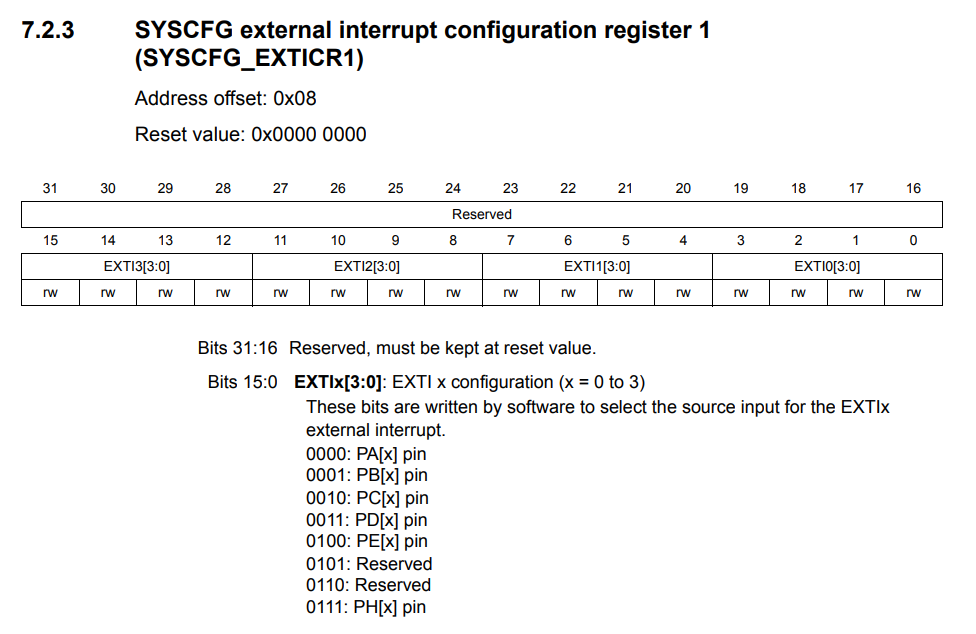
\includegraphics[width=0.8\linewidth]{imagens/SYSCFG_EXTICR1.png}
    \caption{SYSCFG\_EXTICR1}
    \label{fig:syscfg_exticr1}
\end{figure}



Esse registrador serve para funcionar como uma chave seletora (Multiplexador). O microcontrolador não possui uma linha de interrupção individual para cada um de seus dezenas de pinos físicos. Em vez disso, ele agrupa os pinos pelo seu número final (ex: PA13, PB13 e PC13 compartilham a mesma linha física interna, a EXTI13).

Os bits \texttt{EXTIx[3:0]} deste registrador escolhem qual porta vai se conectar àquela linha. É por isso que você não pode ter duas interrupções simultâneas em pinos com o mesmo número (como PA5 e PB5, pois ambos disputam a linha EXTI5), mas pode usar pinos de números diferentes de forma totalmente independente (como PA0 e PB5). No código abaixo, configuramos o \texttt{EXTICR[3]} para conectar a Porta C na linha 13.

\begin{lstlisting}[language=C]
/* main.c */

static void MX_GPIO_Init_Direct(void)
{
  /* 1. Habilita Clocks: GPIOA, GPIOC e SYSCFG (Bit 14 do APB2ENR) */
  /* SYSCFG e obrigatorio para rotear interrupcoes externas */
  RCC->AHB1ENR |= 0x00000005; // Bits 0 (A) e 2 (C) -> 0b101
  RCC->APB2ENR |= 0x00004000; // Bit 14 (SYSCFG EN) -> 0b1 << 14

  /* 2. Configura LED PA5 como Saida */
  GPIOA->MODER &= ~0x00000C00; // Limpa bits 10 e 11 -> (0b1 << 10) | (0b1 << 11)
  GPIOA->MODER |=  0x00000400; // Seta bit 10 (01 = Output)

  /* 3. Configura Botao PC13 como Entrada (MODER bits 26,27 = 00) */
  GPIOC->MODER &= ~0x0C000000; // -> (0b1 << 26) | (0b1 << 27)

  /* 4. Roteamento (SYSCFG) */
  /* Mapeia o pino 13 da Porta C para a linha EXTI13 */
  /* EXTICR[3] controla pinos 12 a 15. A posicao do pino 13 requer o valor 0x2 (Porta C) */
  SYSCFG->EXTICR[3] &= ~0x000000F0; // Limpa nibble do pino 13 -> (~(0b1111 << 4)) 
  // Ele comeca no bit 4 EXTICR4 ou EXTICR[3]
  SYSCFG->EXTICR[3] |=  0x00000020; // Escreve 0010 (Port C) na posicao -> 0b0010 << 4
\end{lstlisting}

O próximo é o controller EXTI, nele vamos alterar os registradores IMR, FTSR e RTSR:

\begin{figure}[H]
    \centering
    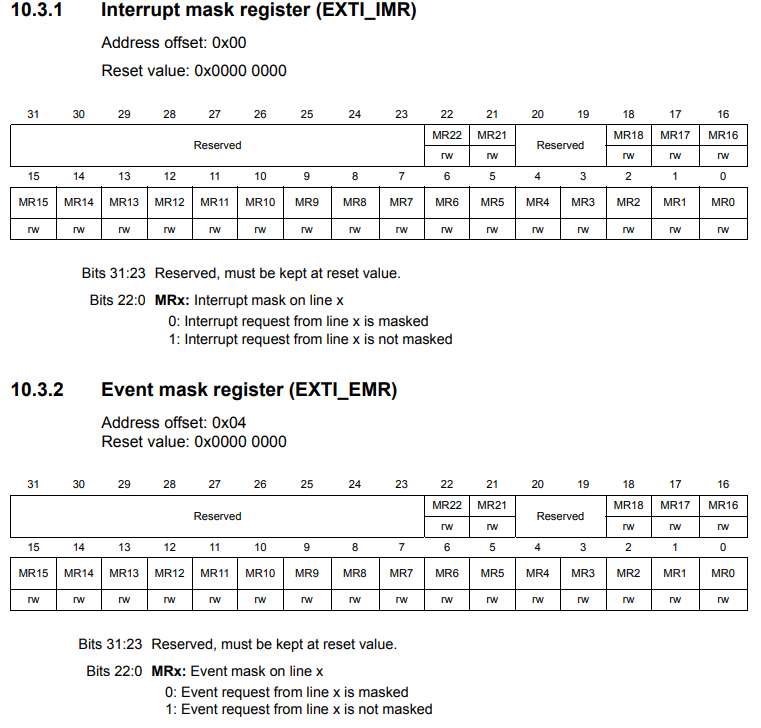
\includegraphics[width=0.8\linewidth]{imagens/EXTI_IMR_EMR.png}
    \caption{EXTI\_IMR e EXTI\_EMR}
\end{figure}

\begin{figure}[H]
    \centering
    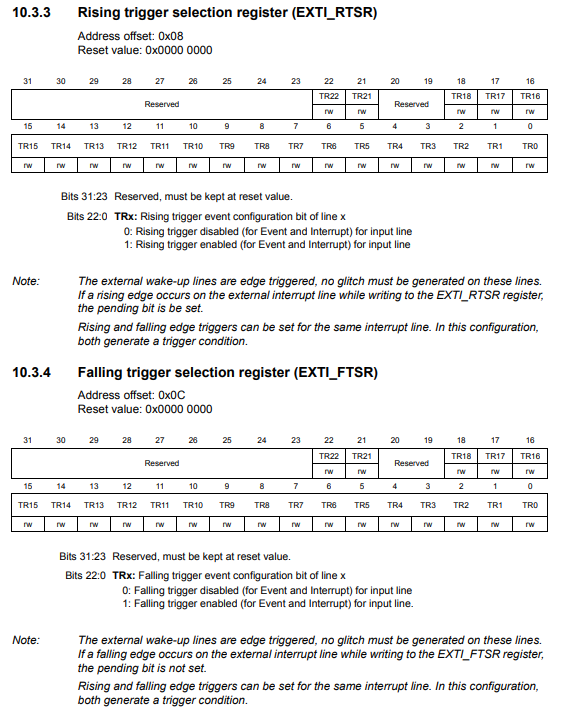
\includegraphics[width=0.8\linewidth]{imagens/EXTI_RTSR_FTSR.png}
    \caption{EXTI\_RTSR e EXTI\_FTSR}
\end{figure}

O que ocorre aqui é que o controlador EXTI recebe o sinal roteado pelo SYSCFG, mas precisamos dizer a ele se e como reagir.

O IMR (Interrupt Mask Register) serve para ``desmascarar'' (habilitar) a linha. Note na imagem que ele possui 23 linhas (MR0 ao MR22). As linhas 0 a 15 são para os pinos físicos (GPIO). As linhas 16 a 22 são conectadas a eventos internos do chip (como alarmes do RTC para acordar o processador), sendo os bits 19 e 20 marcados como reservados (sem conexão física nessa arquitetura).

Os RTSR (Rising) e FTSR (Falling) configuram o gatilho da interrupção. O EXTI não olha o estado estático do pino (se está em 0V ou 3.3V), mas sim a transição da borda. Como queremos detectar quando o botão é pressionado (o sinal cai de ALTO para BAIXO), habilitamos a Borda de Descida (FTSR).

\begin{lstlisting}[language=C]
  /* 5. Configura EXTI (External Interrupt Controller) */
  /* IMR: Interrupt Mask Register - Desmascara a linha 13 */
  EXTI->IMR |= 0x00002000;  // -> 0b1 << 13
  /* FTSR: Falling Trigger Selection - Habilita borda de descida na linha 13 */
  EXTI->FTSR |= 0x00002000;
  /* RTSR: Rising Trigger - Desabilita subida (opcional se quiser garantir) */
  EXTI->RTSR &= ~0x00002000;

  /* 6. Configura NVIC (Core Cortex-M) */
  /* Define prioridade e habilita vetor EXTI15_10 */
  NVIC_SetPriority(EXTI15_10_IRQn, 0);
  NVIC_EnableIRQ(EXTI15_10_IRQn);
}
\end{lstlisting}

\textbf{Nota sobre o NVIC:} As funções \texttt{NVIC\_SetPriority} e \texttt{NVIC\_EnableIRQ} são macros do padrão CMSIS da ARM, portanto, são totalmente válidas mesmo quando não estamos usando a HAL. Por baixo dos panos, elas manipulam os registradores do núcleo Cortex-M:
\begin{itemize}
    \item \texttt{NVIC\_SetPriority} escreve no array de registradores IPR (\textit{Interrupt Priority Register}) para definir a urgência da interrupção.
    \item \texttt{NVIC\_EnableIRQ} escreve no array de registradores ISER (\textit{Interrupt Set-Enable Register}) para finalmente liberar a passagem do sinal para a CPU.
\end{itemize}
Ou seja, como esses registradores são da ARM, precisaríamos procurar a documentação dela para ir atrás do seu funcionamento. Para não encher de muita informação aqui, vou deixar essa parte no \hyperref[anexo:5]{Anexo 5}, caso se interesse por esses detalhes.

Agora é só definir um Handler:

\begin{lstlisting}[language=C]
/* A Rotina de Servico de Interrupcao (ISR) Real */
void EXTI15_10_IRQHandler(void)
{
  /* Verifica se a linha 13 disparou (Pending Register) */
  if (EXTI->PR & 0x00002000)
  {
    /* Limpa a flag escrevendo '1' nela (Sim, escreve 1 para limpar) */
    EXTI->PR = 0x00002000;

    /* Logica: Toggle no pino 5 da porta A (ODR bit 5) */
    GPIOA->ODR ^= 0x00000020;
  }
}
\end{lstlisting}

\subsubsection*{Sobre o Handler:}
Quando você compila seu código, existe um arquivo chamado \texttt{startup\_stm32f4xxxx.s} (escrito em Assembly). Dentro dele, existe a Tabela de Vetores (Vector Table), que diz ao hardware: ``Se a EXTI 13 disparar, procure uma função exatamente com o nome \texttt{EXTI15\_10\_IRQHandler} e execute-a''.

Se o compilador não achar essa função, ele entra em um loop infinito de falha (\texttt{Default\_Handler}). Como você está programando direto nos registradores (Bare Metal), você tem duas opções de como gerenciar isso:

\vspace{0.3cm}
\noindent\textbf{Opção 1: O Jeito Raiz (Recomendado para entender tudo)}\\
Não use o CubeMX para o NVIC. Na interface gráfica, você pode até configurar o pino como entrada/saída para ele gerar as marcações no \texttt{main.h}, mas não marque a caixinha da interrupção na aba do NVIC no CubeMX.
Se você fizer isso, o CubeMX não vai poluir o arquivo \texttt{stm32f4xx\_it.c}. O que você faz então? Você simplesmente digita a função no final do seu próprio \texttt{main.c} ou em um arquivo seu.
O compilador vai achar essa função no \texttt{main.c}, vai conectar o nome dela com a tabela de vetores do Assembly e tudo vai funcionar magicamente. É limpo e você tem 100\% de controle.

\vspace{0.3cm}
\noindent\textbf{Opção 2: O Jeito ``CubeMX Híbrido'' (O que pode dar dor de cabeça)}\\
Se você marcar a interrupção no CubeMX para ele gerar o código, ele vai forçar a criação da função no \texttt{stm32f4xx\_it.c} contendo a chamada da HAL (\texttt{HAL\_GPIO\_EXTI\_IRQHandler}).
Se você simplesmente apagar a linha da HAL e colocar o seu código de registrador lá, quando você for no CubeMX e clicar em ``Generate Code'' de novo no futuro, ele vai apagar a sua lógica e reescrever o código da HAL por cima.
Para evitar que ele apague, você seria obrigado a escrever seu código estritamente entre os comentários de segurança:

\begin{lstlisting}[language=C]
/* No arquivo stm32f4xx_it.c gerado pelo CubeMX */

void EXTI15_10_IRQHandler(void)
{
  /* USER CODE BEGIN EXTI15_10_IRQn 0 */
  if (EXTI->PR & (1UL << 13)) {
      EXTI->PR = (1UL << 13);
      GPIOA->ODR ^= (1UL << 5);
  }
  /* USER CODE END EXTI15_10_IRQn 0 */
  
  // HAL_GPIO_EXTI_IRQHandler(GPIO_PIN_13); <-- Teria que comentar/apagar isso
  
  /* USER CODE BEGIN EXTI15_10_IRQn 1 */
  /* USER CODE END EXTI15_10_IRQn 1 */
}
\end{lstlisting}

Agora, outra dúvida pode surgir:



\subsubsection*{Quem chama o Handler?}
A maior confusão ao aprender interrupções é procurar no código um \texttt{if(botao\_apertado)} que chame a função \texttt{EXTI15\_10\_IRQHandler()}. Essa linha de código não existe. A execução dessa função não é feita por software, mas sim forçada pelo próprio hardware (os transistores) da CPU. Funciona assim:

\begin{enumerate}
    \item O arquivo assembly (\texttt{startup\_stm32f4xxxx.s}) não fica rodando em loop verificando condições. Ele serve apenas para gravar uma lista telefônica fixa no começo da memória Flash: a Tabela de Vetores (Vector Table).
    \item Nessa lista, a posição referente à interrupção do EXTI15\_10 guarda o endereço de memória de onde a sua função foi parar após a compilação.
    \item Quando o sinal elétrico do botão chega ao NVIC, o hardware do núcleo ARM congela a execução do seu \texttt{while(1)} principal automaticamente.
    \item O próprio hardware calcula a posição na Tabela de Vetores, lê o endereço que está guardado lá dentro e o injeta diretamente no \textbf{Program Counter (PC)} do processador. O PC é o registrador que aponta qual é a próxima linha de código que a CPU vai executar.
    \item A CPU sofre um ``teletransporte'' forçado e começa a executar o seu código da ISR instantaneamente.
\end{enumerate}

É por isso que o nome da função no seu \texttt{main.c} deve ser exatamente igual ao que está escrito no arquivo Assembly. Durante a compilação, o Linker procura por esse nome para preencher o endereço correto na Tabela de Vetores. Se houver um erro de digitação, o hardware não vai encontrar o seu código e o microcontrolador irá travar (caindo no loop infinito do \texttt{Default\_Handler}).

E é isso, assim, você conseguiu usar um interrupt em um pino GPIO.

\subsubsection{E se não for GPIO?}

Todo esse processo usando o EXTI serve apenas para eventos externos (pinos) e alguns eventos de \textit{wakeup} específicos.

Se a interrupção for gerada por um periférico interno do microcontrolador (como um Timer estourando, a UART recebendo um dado, ou o ADC finalizando uma leitura), o fluxo não passa pelo EXTI.

Esses periféricos possuem ``vias expressas'' ligadas diretamente ao NVIC. Eles têm suas próprias Flags de interrupção em seus próprios registradores de status, e apontam para vetores dedicados na Tabela de Vetores (como \texttt{TIM2\_IRQHandler} ou \texttt{USART1\_IRQHandler}).

A lógica de prioridade (NVIC) e de limpar a Flag no Handler continua exatamente a mesma, mas a configuração é feita diretamente no periférico. Veremos como habilitar essas interrupções específicas nos capítulos dedicados a cada um deles.

% ==========================================
% HAL FUNCTIONS
% ==========================================
\subsection{HAL Functions}

\begin{figure}[H]
    \centering
    
\includegraphics[width=0.4\linewidth]{imagens/HAL9000.png}
    \caption{HAL9000}
    \label{fig:hal9000}
\end{figure}

\textbf{OBS:} Essa parte pode ser mais complexa de ser entendida, então, é essencial ter entendido os tópicos anteriores.

\textbf{Nota:} \texttt{\_\_weak} é um alias do HAL do qualificador de atributo \texttt{\#define \_\_weak \_\_attribute\_\_((weak))} que, por sua vez, é uma extensão de compilador (comum no GCC) que define um símbolo (função ou variável) como ``fraco''. Ele permite que definições de código do usuário substituam as da biblioteca sem causar erros de nomes duplicados, útil para criar funções padrão que podem ser sobrescritas. Ou seja, o usuário pode ``overridar'' essas funções. Para mais informações \href{https://www.microprogramador.com.br/2022/08/atributos-de-variaveis-em-c.html}{clique aqui}.

A primeira coisa que acontece dentro da função \texttt{main()} gerada pelo CubeMX é a chamada de \texttt{HAL\_Init()}. Sem ela, a biblioteca não funciona. Ela atua como o processo de ``boot'' da abstração de hardware e executa quatro tarefas cruciais em sequência:

\begin{lstlisting}[language=C]
HAL_StatusTypeDef HAL_Init(void)
{
  /* 1. Otimiza o acesso a Flash (Caches e Prefetch) */
#if (INSTRUCTION_CACHE_ENABLE != 0U)
  __HAL_FLASH_INSTRUCTION_CACHE_ENABLE();
#endif /* INSTRUCTION_CACHE_ENABLE */
#if (DATA_CACHE_ENABLE != 0U)
  __HAL_FLASH_DATA_CACHE_ENABLE();
#endif /* DATA_CACHE_ENABLE */
#if (PREFETCH_ENABLE != 0U)
  __HAL_FLASH_PREFETCH_BUFFER_ENABLE();
#endif /* PREFETCH_ENABLE */

  /* 2. Define como as prioridades de interrupcao serao divididas */
  HAL_NVIC_SetPriorityGrouping(NVIC_PRIORITYGROUP_4);

  /* 3. Liga o ``Coracao'' do sistema (SysTick Timer) */
  HAL_InitTick(TICK_INT_PRIORITY);

  /* 4. Inicializa o hardware de baixo nivel (Clocks globais) */
  HAL_MspInit();

  return HAL_OK;
}
\end{lstlisting}

Vamos dissecar os passos 1, 2, 3 e 4.

\subsubsection{HAL\_NVIC\_SetPriorityGrouping(NVIC\_PRIORITYGROUP\_4)}

\begin{lstlisting}[language=C]
void HAL_NVIC_SetPriorityGrouping(uint32_t PriorityGroup)
{
  /* Check the parameters */
  assert_param(IS_NVIC_PRIORITY_GROUP(PriorityGroup));
  /* Set the PRIGROUP[10:8] bits according to the PriorityGroup parameter value */
  NVIC_SetPriorityGrouping(PriorityGroup);
}

void HAL_NVIC_SetPriority(IRQn_Type IRQn, uint32_t PreemptPriority, uint32_t SubPriority)
{
  uint32_t prioritygroup = 0x00U;
  /* Check the parameters */
  assert_param(IS_NVIC_SUB_PRIORITY(SubPriority));
  assert_param(IS_NVIC_PREEMPTION_PRIORITY(PreemptPriority));
  prioritygroup = NVIC_GetPriorityGrouping();
  NVIC_SetPriority(IRQn, NVIC_EncodePriority(prioritygroup, PreemptPriority, SubPriority));
}
\end{lstlisting}

Como vimos no capítulo de interrupções, a STMicroelectronics reserva 4 bits (valores de 0 a 15) para definir a prioridade no NVIC. No entanto, a arquitetura ARM permite que você divida esses 4 bits em duas categorias: \textbf{Preemption Priority} (quem interrompe quem) e \textbf{Subpriority} (critério de desempate).

A função \texttt{HAL\_NVIC\_SetPriorityGrouping} escreve no registrador AIRCR (\textit{Application Interrupt and Reset Control Register}) do núcleo Cortex-M para definir essa divisão.

O CubeMX e a HAL usam o \texttt{Group 4} por padrão. O que isso significa?
\begin{itemize}
    \item \textbf{Group 4:} Todos os 4 bits são usados para \textit{Preemption Priority} (Níveis 0 a 15) e 0 bits para \textit{Subpriority}.
\end{itemize}

Ou seja, no padrão da HAL, não existe critério de desempate complexo. Qualquer interrupção com número menor tem autoridade total para pausar uma interrupção com número maior. Isso é um requisito rigoroso caso você vá usar um Sistema Operacional de Tempo Real (como o FreeRTOS) no futuro.

Lembra da função \texttt{HAL\_NVIC\_SetPriority(IRQn\_Type IRQn, uint32\_t PreemptPriority, uint32\_t SubPriority)}? No caso do \texttt{NVIC\_PRIORITYGROUP\_4}, o valor do \texttt{SubPriority} é ignorado, tudo isso é feito por baixo dos panos pelas funções do CMSIS que dão conta do NVIC, como é o caso do \texttt{NVIC\_EncodePriority} (Veja \hyperref[anexo:5]{Anexo 5}).

\subsubsection{Otimização de Memória (ART Accelerator)}

Logo no início do \texttt{HAL\_Init()}, encontramos a habilitação dos Caches e do Prefetch Buffer:

\begin{lstlisting}[language=C]
#if (INSTRUCTION_CACHE_ENABLE != 0U)
  __HAL_FLASH_INSTRUCTION_CACHE_ENABLE();
#endif /* INSTRUCTION_CACHE_ENABLE */
#if (DATA_CACHE_ENABLE != 0U)
  __HAL_FLASH_DATA_CACHE_ENABLE();
#endif /* DATA_CACHE_ENABLE */
#if (PREFETCH_ENABLE != 0U)
  __HAL_FLASH_PREFETCH_BUFFER_ENABLE();
#endif /* PREFETCH_ENABLE */
\end{lstlisting}

\textbf{Por que isso é necessário?}
Existe um gargalo físico na arquitetura. O núcleo ARM Cortex-M4 pode rodar a velocidades altíssimas (como 84 MHz ou 100 MHz no STM32F411), mas a memória Flash física (onde seu código está gravado) é lenta e só consegue entregar dados confiavelmente a cerca de 30 MHz.

Isso significa que, sem otimização, a cada instrução que a CPU tenta ler da Flash, ela precisa ficar ``congelada'' esperando (os famosos \textit{Wait States}). O código rodaria com menos da metade da velocidade teórica do chip.

Para resolver isso, a ST criou o \textbf{ART Accelerator}:
\begin{itemize}
    \item \textbf{Instruction Cache (I-Cache):} O microcontrolador possui uma pequena quantidade de memória SRAM ultrarrápida acoplada diretamente à CPU. O hardware copia automaticamente as partes do código que estão sendo mais executadas (como o corpo do seu \texttt{while(1)} ou as rotinas matemáticas de controle) da Flash para esse cache. Na próxima iteração, a CPU lê do cache a 100 MHz, sem nenhum atraso.
    \item \textbf{Data Cache (D-Cache):} Faz o mesmo princípio do I-Cache, mas voltado para dados constantes que você declarou no código e que ficam gravados na Flash (como grandes arrays ou tabelas de calibração).
    \item \textbf{Prefetch Buffer:} O hardware ``olha para frente''. Enquanto a CPU está executando a linha 10 do seu código, o Prefetch Buffer já vai fisicamente na memória Flash buscar a linha 11 e a linha 12, deixando-as prontas na porta da CPU antes mesmo de ela pedir.
\end{itemize}

Ao habilitar essas três macros, o STM32 consegue alcançar o que a ST chama de \textit{0-wait state execution performance} (execução com zero espera), garantindo que loops críticos e cálculos de tempo real rodem na velocidade máxima do relógio do sistema.

Aqui está o texto completo e integrado, unindo a arquitetura (Flash vs. RAM) com a solução de hardware (o registrador \texttt{FLASH\_ACR}). Essa junção cria uma narrativa lógica perfeita: o leitor entende onde as coisas estão, qual é o problema físico de acessá-las, e como o código resolve isso.

\vspace{0.3cm}
\noindent\textbf{1. A Arquitetura Harvard Modificada (Onde as coisas vivem?)}\\
Diferente de um PC convencional (que carrega o programa inteiro do HD para a memória RAM antes de rodar), o STM32 trabalha no modelo \textit{Execute In Place (XIP)}. O código roda diretamente de onde está gravado.
O núcleo ARM Cortex-M4 utiliza barramentos (vias de dados) separados para ler instruções e dados:
\begin{itemize}
    \item \textbf{A Flash (O Livro de Receitas):} É a memória não-volátil. Guarda o seu código de máquina (instruções como \texttt{if}, \texttt{while}) e variáveis literais (\texttt{const float PI = 3.14;}). A CPU lê essas informações usando o \textit{I-Bus (Instruction Bus)}.
    \item \textbf{A RAM (A Bancada de Trabalho):} É a memória volátil e ultrarrápida. Guarda tudo o que sofre alteração durante o programa (variáveis globais, o Stack com variáveis locais, etc.). A CPU acessa a RAM usando o \textit{D-Bus (Data Bus)}.
\end{itemize}

\textit{Curiosidade do Startup:} Se a RAM perde tudo ao desligar a placa, como uma variável global \texttt{int contador = 10;} inicia com o valor 10? O arquivo Assembly (\texttt{startup\_stm32.s}) faz uma ponte antes do seu \texttt{main()} começar. Ele vai até a Flash, copia o número ``10'' que o compilador deixou congelado lá, e cola no endereço exato da RAM designado para aquela variável.

\vspace{0.3cm}
\noindent\textbf{2. O Gargalo Físico da Flash}\\
A separação de barramentos é ótima, mas esbarra em um limite físico da engenharia de silício. O núcleo da CPU e a RAM conseguem rodar a velocidades altíssimas (ex: 84 MHz, 100 MHz). No entanto, a memória Flash física é lenta e só consegue entregar dados de forma confiável a cerca de 30 MHz.
Isso significa que, se a sua CPU estiver a 100 MHz, a cada linha de código que ela pedir para a Flash pelo I-Bus, ela precisará ficar ``congelada'' esperando a resposta (os famosos \textit{Wait States}). Isso destruiria a performance do chip.

\vspace{0.3cm}
\noindent\textbf{3. A Solução: ART Accelerator (FLASH\_ACR)}\\
Para resolver esse gargalo, a STMicroelectronics embutiu no controlador da Flash um sistema chamado ART Accelerator (\textit{Adaptive Real-Time memory accelerator}). É ele que o \texttt{HAL\_Init()} configura com as seguintes macros:

\begin{lstlisting}[language=C]
#if (INSTRUCTION_CACHE_ENABLE != 0U)
  __HAL_FLASH_INSTRUCTION_CACHE_ENABLE();
#endif
#if (DATA_CACHE_ENABLE != 0U)
  __HAL_FLASH_DATA_CACHE_ENABLE();
#endif
#if (PREFETCH_ENABLE != 0U)
  __HAL_FLASH_PREFETCH_BUFFER_ENABLE();
#endif
\end{lstlisting}

Essas macros manipulam três bits essenciais do registrador \texttt{FLASH\_ACR} (Access Control Register):
\begin{itemize}
    \item \textbf{Prefetch Buffer (PRFTEN - Bit 8):} O barramento da Flash no STM32 lê blocos largos de 128 bits de uma vez. O Prefetch liga um ``adivinho'': enquanto a CPU está ocupada executando uma linha, o hardware já vai lá na Flash e deixa a próxima instrução engatilhada na porta da CPU.
    \item \textbf{Instruction Cache / I-Cache (ICEN - Bit 9):} O Prefetch é ruim quando o código dá saltos (como voltar ao início de um loop \texttt{while}). O I-Cache liga uma memória SRAM minúscula e ultrarrápida que guarda as instruções desse loop. Na segunda volta do \texttt{while}, a CPU lê a instrução desse cache a 100 MHz, sem nem acordar a Flash.
    \item \textbf{Data Cache / D-Cache (DCEN - Bit 10):} Faz a mesma coisa que o I-Cache, mas no caminho do D-Bus, salvando leituras de constantes e tabelas gravadas na Flash.
\end{itemize}
Ao ativar essas três chaves, o STM32 alcança o estado de \textit{0-wait state execution performance} (execução com zero espera), rodando o código em velocidade máxima.

\vspace{0.3cm}
\noindent\textbf{O Código no ``Bare-Metal''}\\
Ignorando as macros da HAL, a habilitação de todo esse mecanismo de aceleração é feita em uma única linha no início da configuração do relógio do sistema, atacando o registrador ACR:

\begin{figure}[H]
    \centering
    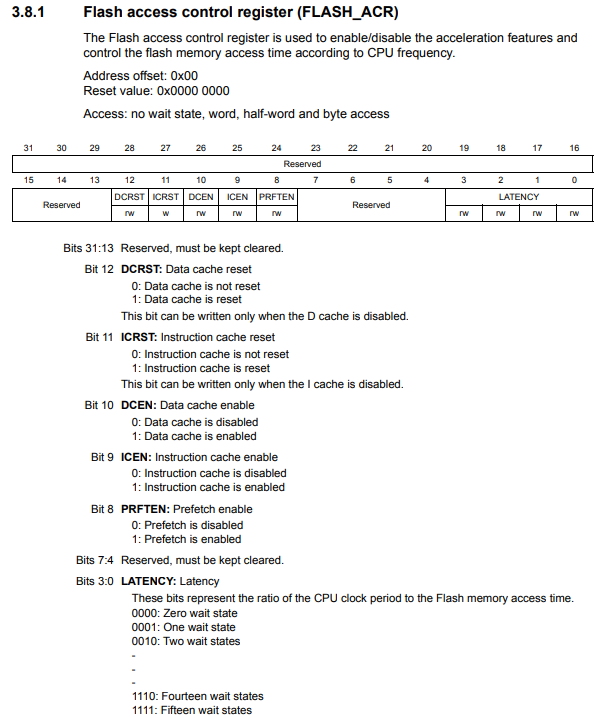
\includegraphics[width=0.8\linewidth]{imagens/FLASH_ACR.png}
    \caption{FLASH\_ACR}
    \label{fig:flash_acr}
\end{figure}

\begin{lstlisting}[language=C]
/* Habilita Prefetch (bit 8), I-Cache (bit 9) e D-Cache (bit 10) simultaneamente */
FLASH->ACR |= (1UL << 8) | (1UL << 9) | (1UL << 10);
\end{lstlisting}

\subsubsection{O SysTick e HAL\_InitTick(TICK\_INT\_PRIORITY)}

\begin{lstlisting}[language=C]
__weak HAL_StatusTypeDef HAL_InitTick(uint32_t TickPriority)
{
  /* Configure the SysTick to have interrupt in 1ms time basis*/
  if (HAL_SYSTICK_Config(SystemCoreClock / (1000U / uwTickFreq)) > 0U)
  {
    return HAL_ERROR;
  }
  /* Configure the SysTick IRQ priority */
  if (TickPriority < (1UL << __NVIC_PRIO_BITS))
  {
    HAL_NVIC_SetPriority(SysTick_IRQn, TickPriority, 0U);
    uwTickPrio = TickPriority;
  }
  else
  {
    return HAL_ERROR;
  }
  /* Return function status */
  return HAL_OK;
}

/**
 * @brief  Initializes the System Timer and its interrupt, and starts the System Tick Timer.
 * Counter is in free running mode to generate periodic interrupts.
 * @param  TicksNumb Specifies the ticks Number of ticks between two interrupts.
 * @retval status:  - 0  Function succeeded.
 * - 1  Function failed.
 */
uint32_t HAL_SYSTICK_Config(uint32_t TicksNumb)
{
  return SysTick_Config(TicksNumb);
}

__STATIC_INLINE uint32_t SysTick_Config(uint32_t ticks)
{
  if ((ticks - 1UL) > SysTick_LOAD_RELOAD_Msk)
  {
    return (1UL);                                                   /* Reload value impossible */
  }
  SysTick->LOAD  = (uint32_t)(ticks - 1UL);                         /* set reload register */
  NVIC_SetPriority (SysTick_IRQn, (1UL << __NVIC_PRIO_BITS) - 1UL); /* set Priority for Systick Interrupt */
  SysTick->VAL   = 0UL;                                             /* Load the SysTick Counter Value */
  SysTick->CTRL  = SysTick_CTRL_CLKSOURCE_Msk |
                   SysTick_CTRL_TICKINT_Msk   |
                   SysTick_CTRL_ENABLE_Msk;                         /* Enable SysTick IRQ and SysTick Timer */
  return (0UL);                                                     /* Function successful */
}
\end{lstlisting}

O microcontrolador precisa de uma noção de tempo para executar tarefas básicas, como o comando \texttt{HAL\_Delay(1000)}. Para isso, a HAL utiliza o \textbf{SysTick}, um timer de 24 bits embutido dentro do próprio núcleo ARM Cortex-M.

A função \texttt{HAL\_InitTick()} faz uma chamada direta para a macro CMSIS \texttt{SysTick\_Config()}. O que ocorre no hardware:
\begin{enumerate}
    \item \textbf{Carga (LOAD):} O registrador de \textit{Reload} do SysTick recebe um valor matemático exato. Como o clock padrão inicial (HSI) costuma ser 16 MHz, o valor carregado é $16.000.000 / 1000 = 16.000$.
    \item \textbf{Contagem:} O SysTick começa a decrementar desse valor até zero a cada ciclo de clock.
    \item \textbf{Interrupção Exclusiva:} Quando chega a zero, ele dispara a interrupção \texttt{SysTick\_Handler()} e recarrega o valor de 16.000 automaticamente.
    \item \textbf{O Resultado:} O \texttt{SysTick\_Handler} é executado rigorosamente a cada 1 milissegundo.
\end{enumerate}

A HAL possui uma variável global chamada \texttt{uwTick}. Dentro desse handler de 1ms, essa variável sofre um \texttt{uwTick++}. Quando você chama \texttt{HAL\_Delay(50)}, a CPU simplesmente entra em um loop \texttt{while} esperando que essa variável \texttt{uwTick} cresça 50 unidades.

O parâmetro \texttt{TICK\_INT\_PRIORITY} garante que a interrupção do SysTick tenha a maior prioridade possível (geralmente 0 ou 15, dependendo da configuração no CubeMX), para que o ``relógio'' do sistema nunca atrase, mesmo se outras interrupções estiverem rodando.

\subsubsection{O MSP e HAL\_MspInit()}

\begin{lstlisting}[language=C]
/* stm32f4xx_hal.c */

__weak void HAL_MspInit(void)
{
  /* NOTE : This function should not be modified, when the callback is needed,
            the HAL_MspInit could be implemented in the user file
   */
}

/* stm32f4xx_hal_msp.c */
void HAL_MspInit(void)
{
  /* USER CODE BEGIN MspInit 0 */
  /* USER CODE END MspInit 0 */
  __HAL_RCC_SYSCFG_CLK_ENABLE();
  __HAL_RCC_PWR_CLK_ENABLE();
  /* System interrupt init*/
  /* USER CODE BEGIN MspInit 1 */
  /* USER CODE END MspInit 1 */
}
\end{lstlisting}

A sigla \textbf{MSP} significa \textit{MCU Specific Package} (Pacote Específico do Microcontrolador).

A filosofia da biblioteca HAL é ser portável. O código de um \texttt{HAL\_Init()} ou de inicialização de UART deve ser idêntico seja em um STM32F4 (alta performance) ou em um STM32G0 (baixo custo). No entanto, os barramentos de energia e clock mudam drasticamente entre famílias diferentes. É aqui que entra o MSP.
\begin{itemize}
    \item \texttt{HAL\_Init()} lida com o núcleo da CPU (comum a todos).
    \item \texttt{HAL\_MspInit()} lida com os registradores do silício específicos do seu chip (Clocks, Power, GPIOs base).
\end{itemize}

Se você abrir o arquivo gerado \texttt{stm32f4xx\_hal\_msp.c}, verá que o \texttt{HAL\_MspInit()} faz o trabalho sujo de ligar o clock do roteador de interrupções (\texttt{\_\_HAL\_RCC\_SYSCFG\_CLK\_ENABLE()}) e o clock de gerenciamento de energia (\texttt{\_\_HAL\_RCC\_PWR\_CLK\_ENABLE()}). Sempre que você inicializa um periférico complexo na HAL (como I2C ou SPI), a HAL chamará uma função \texttt{HAL\_I2C\_MspInit()} por baixo dos panos para ligar os pinos e clocks exatos que aquele periférico precisa no seu chip específico.

Você tocou em um ponto de design arquitetural muito importante do STM32: a \textbf{``Regra de Ouro do Clock''}. No STM32, absolutamente nenhum periférico funciona se o clock dele não for ligado primeiro no barramento correspondente (AHB ou APB). Para economizar bateria, a ST envia o chip com todos os periféricos desligados da energia por padrão.

O arquivo gerado pelo CubeMX coloca as funções \texttt{\_\_HAL\_RCC\_SYSCFG\_CLK\_ENABLE()} e \texttt{\_\_HAL\_RCC\_PWR\_CLK\_ENABLE()} dentro do \texttt{HAL\_MspInit()} porque eles são controladores de sistema, e não periféricos comuns (como uma UART ou um Timer). Eles precisam estar vivos antes de qualquer outra coisa acontecer no chip.

\begin{itemize}
    \item \textbf{Por que o SYSCFG?} Lembra do capítulo de Interrupções Externas (EXTI)? O registrador SYSCFG atua como um ``trilho de trem'', roteando qual pino físico (ex: PA13 ou PC13) vai se conectar à linha EXTI13. Sem ligar o clock do SYSCFG aqui no início, o seu roteamento de interrupções simplesmente não funcionaria. (No Bare-Metal, fizemos isso manualmente com \texttt{RCC->APB2ENR |= (1<<14)}). Veja na documentação da STM para mais informações desse registrador do RCC.
    \item \textbf{Por que o PWR?} O controlador de energia (PWR) gerencia a voltagem do núcleo do microcontrolador. Ele precisa ser acordado agora para que, no próximo passo da inicialização, possamos ajustar a voltagem da CPU para suportar frequências mais altas (como 96 MHz ou 100 MHz).
\end{itemize}

Veremos como funcionam essas funções melhor na próxima sessão.

% ==========================================
% THE CLOCK & TIMERS
% ==========================================
\subsection{The Clock \& Timers}

\begin{figure}[H]
    \centering
    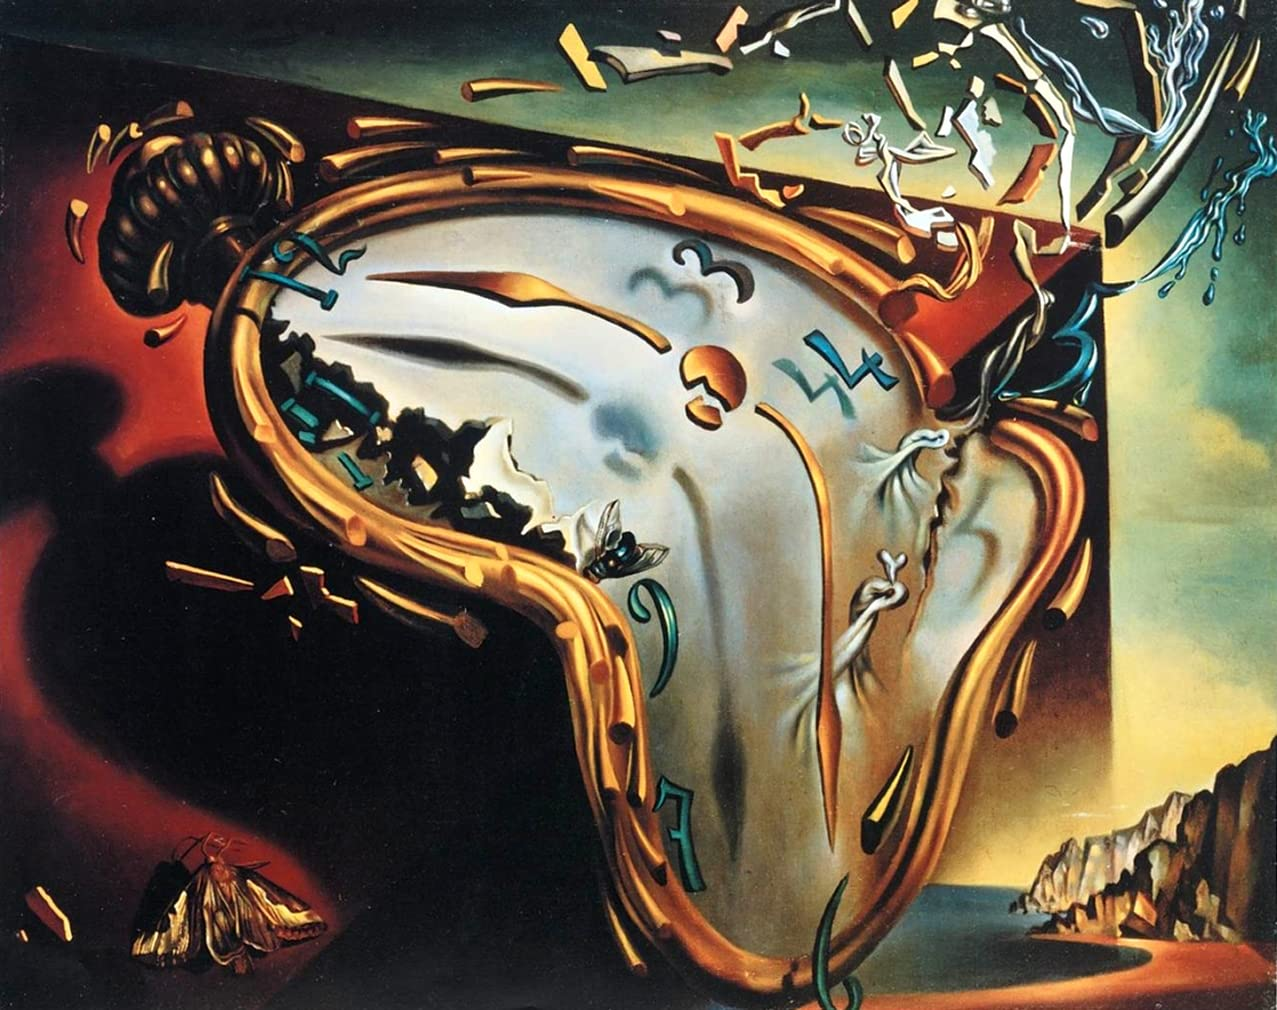
\includegraphics[width=0.6\linewidth]{imagens/Melting_Watch.jpg}
    \caption{Melting Watch, 1954 by Salvador Dali}
    \label{fig:melting_watch}
\end{figure}

\textbf{\texttt{SystemClock\_Config()}:}

\begin{lstlisting}[language=C]
/**
 * @brief System Clock Configuration
 * @retval None
 */
void SystemClock_Config(void)
{
  RCC_OscInitTypeDef RCC_OscInitStruct = {0};
  RCC_ClkInitTypeDef RCC_ClkInitStruct = {0};
  
  /** Configure the main internal regulator output voltage */
  __HAL_RCC_PWR_CLK_ENABLE();
  __HAL_PWR_VOLTAGESCALING_CONFIG(PWR_REGULATOR_VOLTAGE_SCALE1);
  
  /** Initializes the RCC Oscillators according to the specified parameters
   * in the RCC_OscInitTypeDef structure.
   */
  RCC_OscInitStruct.OscillatorType = RCC_OSCILLATORTYPE_HSE;
  RCC_OscInitStruct.HSEState = RCC_HSE_ON;
  RCC_OscInitStruct.PLL.PLLState = RCC_PLL_ON;
  RCC_OscInitStruct.PLL.PLLSource = RCC_PLLSOURCE_HSE;
  RCC_OscInitStruct.PLL.PLLM = 25;
  RCC_OscInitStruct.PLL.PLLN = 192;
  RCC_OscInitStruct.PLL.PLLP = RCC_PLLP_DIV2;
  RCC_OscInitStruct.PLL.PLLQ = 4;
  if (HAL_RCC_OscConfig(&RCC_OscInitStruct) != HAL_OK)
  {
    Error_Handler();
  }
\end{lstlisting}

A função \texttt{SystemClock\_Config()} é literalmente o maestro do seu microcontrolador. Diferente do \texttt{HAL\_Init()}, que é uma função engessada dentro da biblioteca da ST, a \texttt{SystemClock\_Config()} é gerada dinamicamente pelo CubeMX e escrita direto no seu \texttt{main.c}.

Ela é construída com base no que você desenha na aba \textit{Clock Configuration} do CubeMX. Você pode desconstruir esse bloco de código dividindo-o nas três etapas lógicas que ele executa no hardware (RCC - \textit{Reset and Clock Control}). Vamos introduzir com as funções do HAL, depois veremos LL (Bare-Metal).



\subsubsection{Dissecando o SystemClock\_Config()}

\vspace{0.3cm}
\noindent\textbf{1. A Gestão de Energia (Power Regulator)}
\begin{lstlisting}[language=C]
  __HAL_RCC_PWR_CLK_ENABLE();
  __HAL_PWR_VOLTAGESCALING_CONFIG(PWR_REGULATOR_VOLTAGE_SCALE1);
\end{lstlisting}
Antes de acelerar o processador, você precisa garantir que ele tem ``combustível'' suficiente. Sistemas digitais sofrem com um fenômeno físico: quanto mais rápido os transistores ligam e desligam (frequência alta), mais tensão elétrica o núcleo (Core) precisa para se manter estável.
\begin{itemize}
    \item O primeiro comando liga o clock do gerenciador de energia (PWR).
    \item O segundo comando ajusta o regulador de tensão interno para o \textit{Scale 1}. Este é o nível máximo de performance, permitindo que o STM32F4 alcance sua frequência máxima (ex: 100 MHz ou 168 MHz, dependendo da linha). Se fôssemos rodar a 16 MHz para economizar bateria, usaríamos uma escala menor.
\end{itemize}

\vspace{0.3cm}
\noindent\textbf{2. A Fonte do Clock (HSE vs HSI)}
\begin{lstlisting}[language=C]
  RCC_OscInitStruct.OscillatorType = RCC_OSCILLATORTYPE_HSE;
  RCC_OscInitStruct.HSEState = RCC_HSE_ON;
\end{lstlisting}
Todo microcontrolador precisa de um sinal pulsante para funcionar. O STM32 possui duas fontes primárias:
\begin{itemize}
    \item \textbf{HSI (High-Speed Internal):} É um oscilador RC interno (geralmente de 16 MHz). Ele liga rápido e não custa nada, mas é instável e sua frequência varia com a temperatura do chip.
    \item \textbf{HSE (High-Speed External):} É o cristal de quartzo soldado na sua placa de desenvolvimento (geralmente de 8 MHz ou 25 MHz). Ele é absurdamente preciso.
\end{itemize}
No código gerado, estamos dizendo ao hardware: ``Ligue o oscilador externo (HSE), pois precisamos de precisão''. (A precisão do HSE é obrigatória se você for usar portas USB ou comunicação UART em altas velocidades).

\vspace{0.3cm}
\noindent\textbf{3. O PLL (Phase-Locked Loop): A Caixa de Marchas}
\begin{lstlisting}[language=C]
  RCC_OscInitStruct.PLL.PLLState = RCC_PLL_ON;
  RCC_OscInitStruct.PLL.PLLSource = RCC_PLLSOURCE_HSE;
  RCC_OscInitStruct.PLL.PLLM = 25;
  RCC_OscInitStruct.PLL.PLLN = 192;
  RCC_OscInitStruct.PLL.PLLP = RCC_PLLP_DIV2;
  RCC_OscInitStruct.PLL.PLLQ = 4;
\end{lstlisting}

O cristal da placa (HSE) geralmente tem 25 MHz (comum nas placas Black Pill). Mas nós queremos que o chip rode a 96 MHz ou 100 MHz. Como resolvemos isso? Usando o PLL.

O PLL é um multiplicador de frequência embutido no hardware. Ele pega uma frequência baixa e a ``estica'' para uma frequência alta usando uma fórmula matemática configurada por esses divisores:
\begin{itemize}
    \item \textbf{PLL Source:} Dizemos ao PLL para engolir o sinal do cristal (HSE).
    \item \textbf{PLLM (Divisor de Entrada):} Divide os 25 MHz do cristal por 25. Resultado = 1 MHz. (O PLL precisa de um sinal ``limpo'' de 1 a 2 MHz na entrada).
    \item \textbf{PLLN (Multiplicador Principal):} Pega esse 1 MHz e multiplica por 192. O oscilador interno do PLL agora está vibrando a 192 MHz (chamado de $F_{VCO}$).
    \item \textbf{PLLP (Divisor do Sistema):} Pega os 192 MHz e divide por 2 (\texttt{RCC\_PLLP\_DIV2}). Resultado final: \textbf{96 MHz}. Este é o seu \texttt{SYSCLK} real, a velocidade que a sua CPU vai rodar.
    \item \textbf{PLLQ (Divisor USB):} Pega os mesmos 192 MHz e divide por 4. Resultado = 48 MHz. Essa frequência é um requisito físico estrito, exigido pelo hardware da porta USB e do gerador de números aleatórios (RNG) para funcionar.
\end{itemize}

Ao final, a função \texttt{HAL\_RCC\_OscConfig(\&RCC\_OscInitStruct)} pega toda essa struct (que estava apenas na RAM) e escreve seus valores nos registradores físicos \texttt{RCC->CR} e \texttt{RCC->PLLCFGR}, forçando o hardware a aplicar a nova velocidade.

Esta explicação cobre a primeira metade do código do Clock. Logo após essa etapa de osciladores, o \texttt{SystemClock\_Config()} costuma ter outro bloco de código preenchendo uma struct chamada \texttt{RCC\_ClkInitStruct} e chamando \texttt{HAL\_RCC\_ClockConfig()}.

\subsubsection{A Distribuição do Clock: AHB e APB}

A CPU não trabalha sozinha. Ela precisa se comunicar com a memória Flash, RAM, e os periféricos (GPIO, Timers, UART). Essa comunicação acontece através de ``rodovias'' chamadas \textit{Buses} (Barramentos). É nessa etapa que vamos definir a velocidade dessas ``rodovias''.

Aqui está o código gerado pelo CubeMX para essa etapa:
\begin{lstlisting}[language=C]
  /* 4. Configuracao dos Barramentos (Buses) e Latencia da Flash */
  RCC_ClkInitStruct.ClockType = RCC_CLOCKTYPE_HCLK | RCC_CLOCKTYPE_SYSCLK
                              | RCC_CLOCKTYPE_PCLK1 | RCC_CLOCKTYPE_PCLK2;
  RCC_ClkInitStruct.SYSCLKSource = RCC_SYSCLKSOURCE_PLLCLK;
  RCC_ClkInitStruct.AHBCLKDivider = RCC_SYSCLK_DIV1;
  RCC_ClkInitStruct.APB1CLKDivider = RCC_HCLK_DIV2;
  RCC_ClkInitStruct.APB2CLKDivider = RCC_HCLK_DIV1;

  if (HAL_RCC_ClockConfig(&RCC_ClkInitStruct, FLASH_LATENCY_3) != HAL_OK)
  {
    Error_Handler();
  }
\end{lstlisting}

\vspace{0.3cm}
\noindent\textbf{1. Selecionando a Fonte Principal (SYSCLKSource)}
\begin{lstlisting}[language=C]
  RCC_ClkInitStruct.SYSCLKSource = RCC_SYSCLKSOURCE_PLLCLK;
\end{lstlisting}

Lembra que ligamos o PLL e o fizemos gerar 96 MHz na etapa anterior? Este comando é o momento exato em que viramos a ``chave'' geral do chip. Estamos dizendo: ``A partir de agora, o System Clock (SYSCLK) deixa de usar o HSI lento e passa a usar o sinal turbinado do PLL''.

\vspace{0.3cm}
\noindent\textbf{2. O Barramento AHB (Advanced High-performance Bus)}
\begin{lstlisting}[language=C]
  RCC_ClkInitStruct.AHBCLKDivider = RCC_SYSCLK_DIV1;
\end{lstlisting}

O AHB é a via expressa principal do microcontrolador. Ele conecta a CPU à Memória Flash, SRAM e ao controlador de DMA. O clock que corre aqui é chamado de HCLK.
Ao usar \texttt{DIV1} (Divisor por 1), estamos dizendo que a CPU e as memórias vão rodar na velocidade máxima do \texttt{SYSCLK} (os mesmos 96 MHz).

\vspace{0.3cm}
\noindent\textbf{3. Os Barramentos APB (Advanced Peripheral Bus)}
\begin{lstlisting}[language=C]
  RCC_ClkInitStruct.APB1CLKDivider = RCC_HCLK_DIV2;
  RCC_ClkInitStruct.APB2CLKDivider = RCC_HCLK_DIV1;
\end{lstlisting}

Os periféricos (Timers, I2C, SPI) não ficam pendurados na via expressa AHB. Eles ficam em vias marginais chamadas APB. A arquitetura divide isso em duas:
\begin{itemize}
    \item \textbf{APB1 (Low-Speed):} É onde moram periféricos mais lentos (I2C, UARTs secundárias, Timers básicos). No STM32F411, esse barramento tem um limite físico de velocidade (geralmente 50 MHz). Como nosso AHB está a 96 MHz, somos obrigados a usar o \texttt{DIV2} (Divisor por 2) para que o APB1 rode a seguros 48 MHz. Esse clock é chamado de \texttt{PCLK1}.
    \item \textbf{APB2 (High-Speed):} É onde moram periféricos rápidos (SPI1, UART1, ADC). Esse barramento suporta a velocidade máxima do chip (100 MHz). Portanto, podemos usar \texttt{DIV1}, fazendo-o rodar aos mesmos 96 MHz da CPU. Esse clock é o \texttt{PCLK2}.
\end{itemize}

\textit{Nota Prática para Timers:} Uma peculiaridade da arquitetura STM32 é que, se o divisor do APB for diferente de 1 (como no APB1), o hardware \textbf{automaticamente multiplica o clock dos Timers por 2}. Portanto, mesmo que o barramento APB1 esteja a 48 MHz, os Timers pendurados nele receberão 96 MHz. Isso é crucial na hora de calcular os Prescalers no código.

\vspace{0.3cm}
\noindent\textbf{4. O ``Assassino Silencioso'': Flash Latency (Wait States)}
\begin{lstlisting}[language=C]
  if (HAL_RCC_ClockConfig(&RCC_ClkInitStruct, FLASH_LATENCY_3) != HAL_OK)
\end{lstlisting}

Este é um dos conceitos mais importantes do hardware. A memória Flash (onde seu código C está gravado) é fisicamente construída de forma que sua leitura é lenta. Ela só consegue fornecer dados de forma confiável a cerca de 30 MHz.

Se a CPU está rodando a 96 MHz e pede uma instrução para a Flash, a Flash não consegue entregar a tempo. Se a CPU tentar ler assim mesmo, ela lerá ``lixo'' e o microcontrolador vai travar (\textit{Hard Fault}) instantaneamente.

A solução é o Flash Latency (ou Wait States). O parâmetro \texttt{FLASH\_LATENCY\_3} diz à CPU: ``Toda vez que você pedir algo para a Flash, congele e espere 3 ciclos de clock de braços cruzados até o dado ficar pronto''. 

A regra geral da ST é: adicione 1 Wait State a cada $\sim$30 MHz de aumento no SYSCLK. A função \texttt{HAL\_RCC\_ClockConfig} aplica todas essas velocidades aos barramentos e configura a memória Flash simultaneamente.

Pronto, utilizando o HAL, é isso. Agora, configurar a árvore de clock inteira (HSE, PLL, Flash, AHB/APB) via registradores é, de longe, a parte mais sequencial e rigorosa do Bare Metal. Se você errar a ordem (por exemplo, acelerar a CPU antes de configurar a latência da Flash), o processador trava instantaneamente.

\subsubsection{System Clock ``No Osso'' (Sem HAL)}

Para fazer exatamente o que a \texttt{SystemClock\_Config()} gerada pelo CubeMX faz (levar o chip de 16 MHz internos para 96 MHz via cristal externo), precisamos seguir uma ``receita de bolo'' estrita no hardware.

Esta é a sequência exata de registradores que devemos manipular:
\begin{lstlisting}[language=C]
/* ========================================================== */
/* CONFIGURACAO DO CLOCK VIA REGISTRADORES (Bare Metal)       */
/* Objetivo: 96 MHz usando cristal HSE de 25 MHz              */
/* ========================================================== */
void clockInitDirect(void)
{
  /* 1. Ligar o Cristal Externo (HSE) e aguardar estabilizar */
  RCC->CR |= (1UL << 16); // Seta o bit HSEON
  while (!(RCC->CR & (1UL << 17))); // Fica preso aqui ate o bit HSERDY virar 1

  /* 2. Configurar a Energia (Regulador Interno para Scale 1) */
  RCC->APB1ENR |= (1UL << 28); // Liga o clock do periferico de energia (PWREN)
  PWR->CR |= (3UL << 14);      // Seta os bits VOS[1:0] para 11 (Scale 1 = Max Performance)

  /* 3. Configurar os Barramentos AHB e APB (Prescalers) */
  /* AHB = DIV1 (000), APB2 = DIV1 (000). So precisamos mudar o APB1 para DIV2 (100) */
  RCC->CFGR |= (4UL << 10); // Bits PPRE1[2:0] = 100 (Divide APB1 por 2)

  /* 4. Configurar o PLL (A Caixa de Marchas) */
  /* Formula: fVCO = (HSE / M) * N.  SYSCLK = fVCO / P.
   * Valores: M = 25, N = 192, P = 2, Q = 4
   * Bit 22 = 1 (Fonte do PLL e o HSE) */
  RCC->PLLCFGR = (4UL << 24)       | // PLLQ = 4
                 (1UL << 22)       | // PLLSRC = HSE
                 (0UL << 16)       | // PLLP = 2 (00 significa DIV2)
                 (192UL << 6)      | // PLLN = 192
                 (25UL << 0);        // PLLM = 25

  /* 5. Ligar o PLL e aguardar o ``Lock'' (estabilizacao) */
  RCC->CR |= (1UL << 24); // Seta o bit PLLON
  while (!(RCC->CR & (1UL << 25))); // Aguarda o bit PLLRDY virar 1

  /* 6. Configurar a Latencia da Flash (MUITO IMPORTANTE) */
  /* Se pularmos isso, a CPU vai tentar ler a Flash a 96MHz, nao vai conseguir e vai travar. */
  /* Precisamos de 3 Wait States (LATENCY = 011), alem de ligar Caches e Prefetch */
  FLASH->ACR = (1UL << 10) | // DCEN (Data Cache Enable)
               (1UL << 9)  | // ICEN (Instruction Cache Enable)
               (1UL << 8)  | // PRFTEN (Prefetch Enable)
               (3UL << 0);   // LATENCY = 3 Wait States

  /* 7. Virar a chave: Dizer ao sistema para usar o PLL como fonte principal */
  RCC->CFGR |= (2UL << 0); // Bits SW[1:0] = 10 (Seleciona o PLL)
  while ((RCC->CFGR & (3UL << 2)) != (2UL << 2)); // Aguarda o status confirmar a mudanca
}
\end{lstlisting}

\subsubsection{Timers Básicos (Hardware Timers)}

Um Timer de hardware nada mais é do que um contador digital estúpido e muito rápido. Ele recebe os pulsos de clock do barramento APB (que configuramos no \texttt{SystemClock\_Config()}) e soma +1 a um registrador até atingir um limite, quando então ele ``estoura'' (gera um evento ou interrupção) e volta a zero.

Para dominar os Timers, você precisa entender apenas três registradores principais:

\begin{figure}[H]
    \centering
    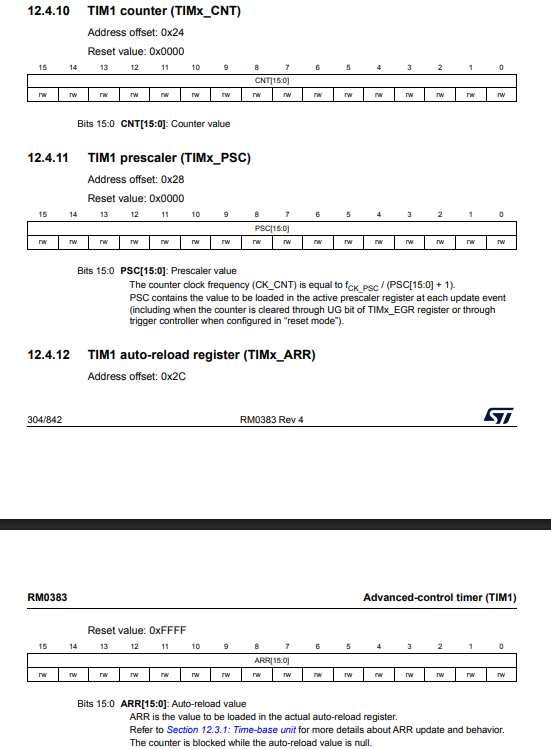
\includegraphics[width=0.8\linewidth]{imagens/TIMx_CNT_PSC_ARR.png}
    \caption{TIMx\_CNT, TIMx\_PSC e TIMx\_ARR}
    \label{fig:timx_cnt_psc_arr}
\end{figure}

\begin{itemize}
    \item \textbf{CNT (Counter):} É o registrador que efetivamente conta (0, 1, 2, 3...).
    \item \textbf{PSC (Prescaler):} O clock do APB é rápido demais (ex: 96 MHz). O Prescaler atua como um freio. Se você colocar um Prescaler de 96, o Timer só vai somar +1 no CNT a cada 96 pulsos do APB. Isso reduz a frequência de contagem para 1 MHz.
    \item \textbf{ARR (Auto-Reload Register):} É o limite máximo. O Timer conta do 0 até o valor definido no ARR. Quando atinge o ARR, ocorre o \textit{Update Event} (Estouro), a interrupção é gerada, e o CNT volta a zero automaticamente.
\end{itemize}

\vspace{0.3cm}
\noindent\textbf{A Matemática do Timer}\\

Para configurar um Timer que estoure exatamente a cada 1 segundo (1 Hz) ou 1 milissegundo (1000 Hz), usamos a seguinte fórmula:

\[ f_{update} = \frac{f_{TIMx\_CLK}}{(PSC + 1) \times (ARR + 1)} \]

O ``+1'' existe na fórmula porque os registradores começam a contar do 0 no hardware.

\textbf{Exemplo Prático:} Queremos uma interrupção a cada 1 segundo (1 Hz) usando o TIM2, sabendo que ele está pendurado no APB1 rodando a 96 MHz.
\begin{itemize}
    \item $f_{TIMx\_CLK} = 96.000.000$ Hz
    \item Escolhemos $PSC = 95.999$ (Isso reduz o clock para 1.000 Hz, ou seja, 1 pulso por milissegundo).
    \item Escolhemos $ARR = 999$ (O contador vai até 999, completando 1000 ciclos).
\end{itemize}

\[ f_{update} = \frac{96.000.000}{(95999 + 1) \times (999 + 1)} = \frac{96.000.000}{96.000.000} = 1 \text{ Hz} \]

\vspace{0.3cm}
\noindent\textbf{Comandos Básicos (HAL\_TIM)}\\
Na biblioteca HAL, após configurar o timer no CubeMX (definindo o PSC e ARR), você precisa ligá-lo no \texttt{main()}.

\textbf{1. Modo Polling (Travando a CPU):}\\
Inicia o Timer, mas você precisa ficar olhando o registrador de flag manualmente para saber se estourou.
\begin{lstlisting}[language=C]
HAL_TIM_Base_Start(&htim2); 
\end{lstlisting}

\textbf{2. Modo Interrupt (O jeito certo):}\\
Inicia o Timer e avisa ao NVIC: ``Quando o ARR for atingido, me avise''.
\begin{lstlisting}[language=C]
/* Inicie isso apenas uma vez, antes do while(1) */
HAL_TIM_Base_Start_IT(&htim2);
\end{lstlisting}

\vspace{0.3cm}
\noindent\textbf{O Callback (A ISR do Timer)}\\
Lembra do ``E se não for GPIO?'' do capítulo de interrupções? Aqui está a resposta. Quando o Timer estoura, o NVIC para a CPU e pula para o \texttt{TIM2\_IRQHandler()}. Dentro dele, a HAL limpa a flag de estouro e chama um Callback específico de Timer, o \texttt{HAL\_TIM\_PeriodElapsedCallback}.

Basta você criar essa função no seu \texttt{main.c}:
\begin{lstlisting}[language=C]
/* Esta funcao e chamada automaticamente sempre que QUALQUER Timer estourar */
void HAL_TIM_PeriodElapsedCallback(TIM_HandleTypeDef *htim)
{
  /* Precisamos verificar QUEM chamou, pois todos os Timers caem aqui */
  if (htim->Instance == TIM2) 
  {
    /* Logica a ser executada a cada 1 segundo */
    HAL_GPIO_TogglePin(GPIOA, GPIO_PIN_5); 
  }
}
\end{lstlisting}

\textbf{Por que usar isso em vez do \texttt{HAL\_Delay()}?}\\
Se você usa \texttt{HAL\_Delay(1000)} no \texttt{while(1)}, a sua CPU fica 100\% do tempo presa rodando em círculos, incapaz de ler botões ou receber dados da UART.
Se você usa um Hardware Timer com Interrupção, o seu \texttt{while(1)} fica livre para processar telas, calcular dados e escutar sensores. A CPU só gasta 1 microssegundo do tempo dela a cada 1 segundo para ir lá piscar o LED e voltar. A ideia é a mesma do \texttt{millis()} vs \texttt{delay()} do Arduino.

\subsubsection{Timers direto nos Registradores (Bare Metal)}
Esquecer a HAL para os Timers simplifica muito o código. Lembra da trindade dos registradores do Timer (CNT, PSC e ARR)? A configuração exige apenas setar os limites, habilitar o sinal de interrupção interno e ligar o contador. Aqui estão os outros registradores utilizados:

\begin{figure}[H]
    \centering
    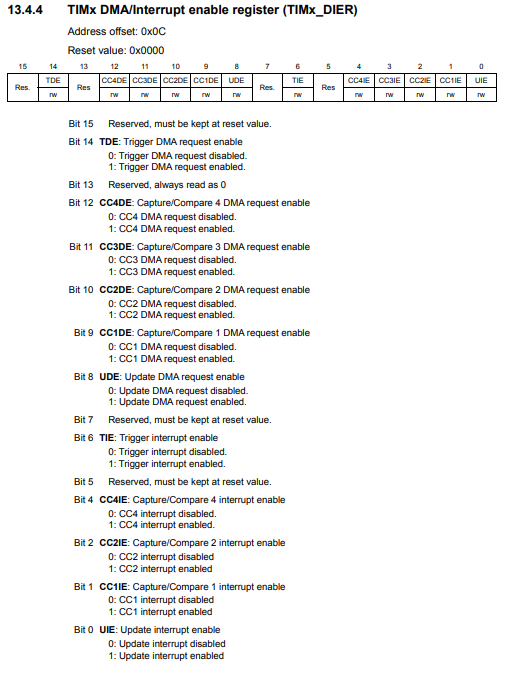
\includegraphics[width=0.8\linewidth]{imagens/TIMx_DIER.png}
    \caption{TIMx\_DIER}
\end{figure}

\begin{figure}[H]
    \centering
    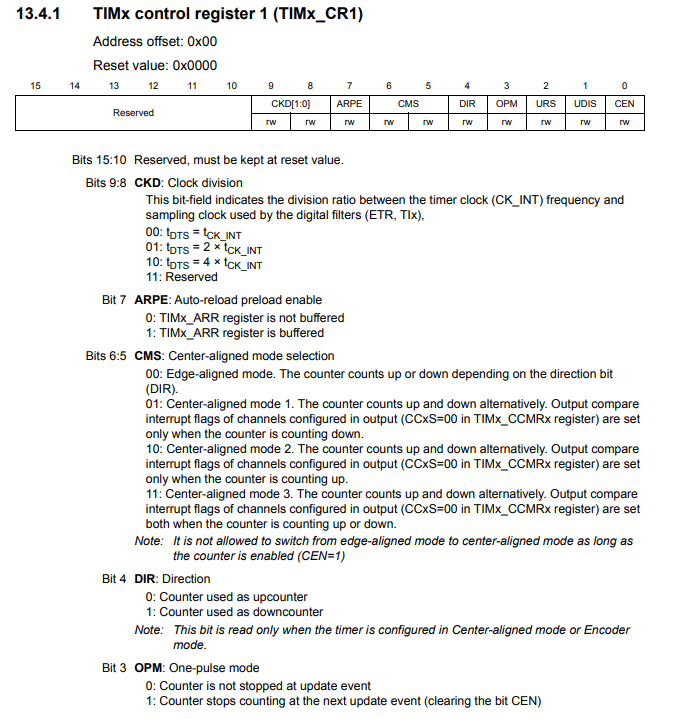
\includegraphics[width=0.8\linewidth]{imagens/TIMx_CR1.png}
    \caption{TIMx\_CR1}
\end{figure}

\begin{figure}[H]
    \centering
    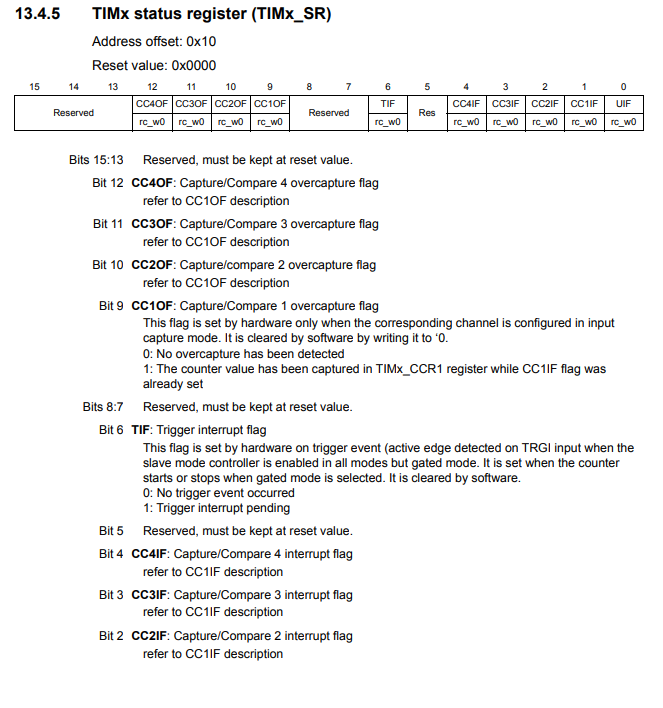
\includegraphics[width=0.8\linewidth]{imagens/TIMx_SR_1.png}
    \caption{TIMx\_SR\_1}
\end{figure}

\begin{figure}[H]
    \centering
    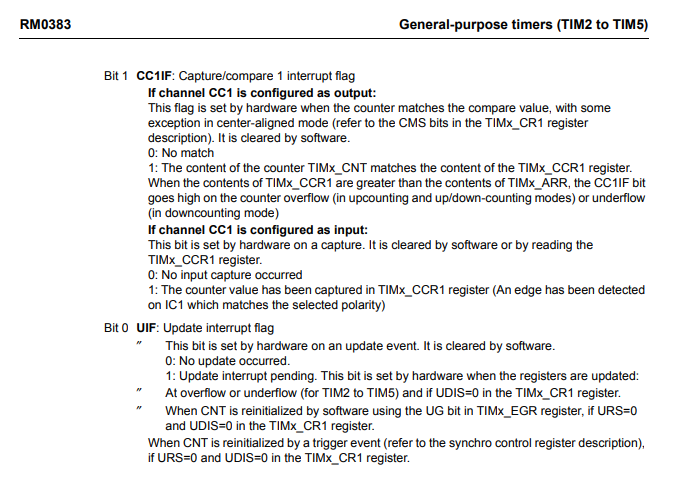
\includegraphics[width=0.8\linewidth]{imagens/TIMx_SR_2.png}
    \caption{TIMx\_SR\_2}
\end{figure}

Aqui está como configuramos o TIM2 para gerar uma interrupção a cada 1 segundo (assumindo clock de 96 MHz no barramento dele):

\begin{lstlisting}[language=C]
/* ========================================================== */
/* CONFIGURACAO DO TIM2 VIA REGISTRADORES (1 Segundo)         */
/* ========================================================== */
void timer2InitDirect(void)
{
  /* 1. Ligar o Clock do TIM2 no barramento APB1 */
  RCC->APB1ENR |= (1UL << 0); // Bit TIM2EN

  /* 2. Configurar o Freio (Prescaler) e o Limite (Auto-Reload) */
  /* A formula pede valor - 1. Portanto, 96000 - 1 = 95999. */
  TIM2->PSC = 95999; 
  TIM2->ARR = 999;   // 1000 ciclos - 1

  /* 3. Habilitar a interrupcao interna de ``Estouro'' (Update Event) */
  TIM2->DIER |= (1UL << 0); // Seta o bit UIE (Update Interrupt Enable)

  /* 4. Ligar o Timer! */
  TIM2->CR1 |= (1UL << 0); // Seta o bit CEN (Counter Enable)

  /* 5. Avisar ao NVIC para deixar o sinal passar (Usando CMSIS) */
  NVIC_EnableIRQ(TIM2_IRQn);
}

/* ========================================================== */
/* A ROTINA DE SERVICO DE INTERRUPCAO (O Callback Direto)     */
/* ========================================================== */
void TIM2_IRQHandler(void)
{
  /* Verifica se a flag de ``Update'' (UIF) realmente foi levantada */
  if (TIM2->SR & (1UL << 0))
  {
    /* Obrigatorio: Limpar a flag escrevendo ZERO nela */
    /* Diferente do EXTI que limpa com '1', o SR do Timer limpa com '0' */
    TIM2->SR &= ~(1UL << 0); 

    /* SUA LOGICA AQUI: Toggle no LED, etc. */
    GPIOA->ODR ^= (1UL << 5); 
  }
}
\end{lstlisting}

\subsubsection{PWM (Pulse Width Modulation)}
O microcontrolador é uma criatura puramente digital: seus pinos só conseguem cuspir 3.3V (ALTO) ou 0V (BAIXO). Ele não consegue gerar 1.5V, por exemplo.

Para contornar isso, usamos o PWM (Modulação por Largura de Pulso). A ideia é ligar e desligar o pino tão rápido que o dispositivo conectado (um motor ou um LED) ``sente'' apenas a tensão média.
Se o pino ficar 50\% do tempo ligado e 50\% desligado (\textit{Duty Cycle} de 50\%), a tensão média aparente será de 1.65V.

\begin{figure}[H]
    \centering
    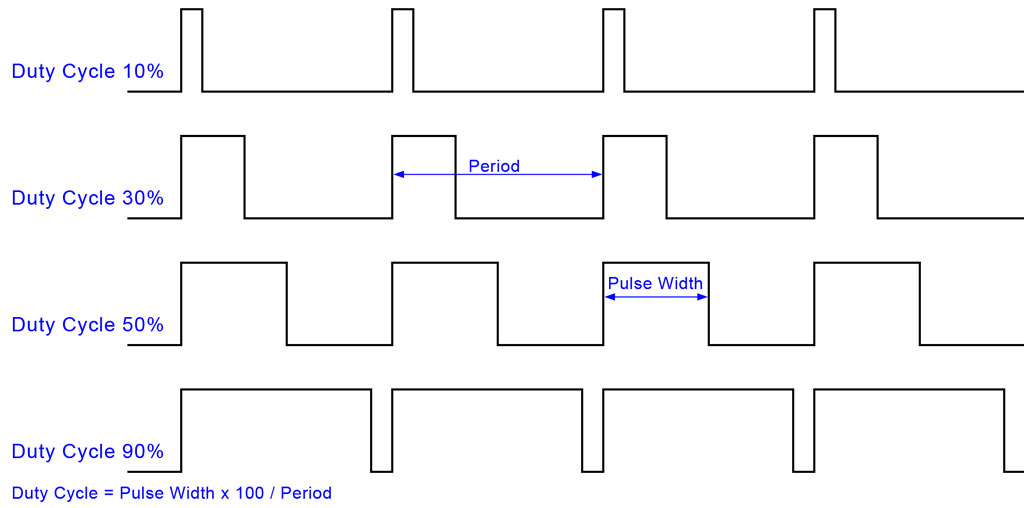
\includegraphics[width=0.8\linewidth]{imagens/PWM.jpg}
    \caption{PWM}
    \label{fig:pwm}
\end{figure}



\vspace{0.3cm}
\noindent\textbf{A Mágica do Hardware: ARR e CCR}\\
No STM32, o PWM é gerado pelos Timers (TIM2, TIM3, etc.). Cada Timer de propósito geral costuma ter 4 ``Canais'' de saída (CH1 a CH4), o que significa que um único Timer pode gerar 4 sinais de PWM independentes.

Para o PWM funcionar, o hardware do Timer faz uma comparação constante entre três registradores:
\begin{itemize}
    \item \textbf{CNT (Counter):} É o cronômetro girando, contando de 0 para cima.
    \item \textbf{ARR (Auto-Reload Register):} Define o ``teto'' da contagem. É ele quem dita a \textbf{Frequência} (o Período) do seu PWM. Quando o CNT atinge o ARR, ele zera e o ciclo recomeça.
    \item \textbf{CCR (Capture/Compare Register):} É a estrela do PWM. Cada canal tem o seu (CCR1, CCR2, etc.). Ele dita o \textbf{Duty Cycle} (o tempo em nível ALTO).
\end{itemize}

\textbf{A Lógica Interna (PWM Mode 1):}
\begin{itemize}
    \item Enquanto o cronômetro for menor que o valor de corte ($CNT < CCR$), o pino físico fica em ALTO (3.3V).
    \item Quando o cronômetro ultrapassa o valor de corte ($CNT \ge CCR$), o pino físico cai para BAIXO (0V) até o fim do ciclo.
\end{itemize}

\vspace{0.3cm}
\noindent\textbf{A Frequência vs. O Duty Cycle}\\
Para entender o PWM, você precisa separar dois conceitos absolutos:
\begin{itemize}
    \item \textbf{A Frequência (Período):} É a ``janela de tempo'' fixa em que a onda se repete. Se a frequência é 50 Hz, significa que o ciclo inteiro dura exatos 20 ms. A frequência dita o ritmo básico (se o LED vai piscar perceptivelmente ou se o servo motor vai reconhecer o sinal).
    \item \textbf{O Duty Cycle (Ciclo de Trabalho):} É a porcentagem de tempo, dentro dessa janela fixa, em que o pino fica ligado (ALTO). Se o Duty Cycle for 50\% num período de 20 ms, o pino fica 10 ms em ALTO e 10 ms em BAIXO. A tensão média sentida é a metade (1.65V).
\end{itemize}

\vspace{0.3cm}
\noindent\textbf{A Matemática (Exemplo Prático)}\\
Como chegamos nos valores reais? Precisamos domar o Clock do sistema usando o Prescaler (PSC) e o ARR.

\textbf{1. Frequência do PWM:}
\[ F_{PWM} = \frac{F_{Clock}}{(PSC + 1) \times (ARR + 1)} \]
Exemplo: O barramento do seu timer roda a 84 MHz (84.000.000). Você quer controlar um Servo Motor que exige exatamente 50 Hz. Como fazemos a conta?
\begin{itemize}
    \item \textbf{Passo 1 (PSC):} Primeiro, reduzimos o clock insano para algo contável. Escolhemos um PSC de 83. A fórmula divide os 84 MHz por $(83 + 1)$. O Timer agora ``bate'' a 1 MHz ($1.000.000$ vezes por segundo).
    \item \textbf{Passo 2 (ARR):} Agora, pegamos esse Timer rodando a 1 MHz e definimos o limite de contagem (ARR). Se dividirmos $1.000.000$ por 50 Hz, precisamos contar até $20.000$. Então, definimos o ARR como 19999 (pois conta do 0).
\end{itemize}

\textbf{2. Duty Cycle:}
\[ Duty(\%) = \left( \frac{CCR}{ARR + 1} \right) \times 100 \]
Sabendo que o seu ARR vai de 0 a 19999 (um total de 20.000 ``passos''), se você quiser um Duty Cycle de 10\% (pino ligado por 10\% do tempo), basta configurar o CCR para 2000.

\vspace{0.3cm}
\noindent\textbf{Com HAL (A Função e a Macro)}\\
No CubeMX, você configura o Timer escolhendo o \textit{Clock Source} como \textit{Internal Clock} e no \textit{Channel 1} você seleciona \textit{PWM Generation CH1}.

O código gerado fará todo o setup da struct \texttt{htimx}. Para fazer o PWM funcionar no seu \texttt{main.c}, você só precisa de duas linhas.
\begin{lstlisting}[language=C]
/* Inicia a geracao do PWM no Canal 1 do Timer 2 */
HAL_TIM_PWM_Start(&htim2, TIM_CHANNEL_1);

while (1)
{
  /* Altera a largura do pulso (Duty Cycle) em tempo real */
  /* A macro __HAL_TIM_SET_COMPARE escreve direto no registrador CCR1 */
  __HAL_TIM_SET_COMPARE(&htim2, TIM_CHANNEL_1, 1500); 
  HAL_Delay(1000);
  
  __HAL_TIM_SET_COMPARE(&htim2, TIM_CHANNEL_1, 2000);
  HAL_Delay(1000);
}
\end{lstlisting}

\vspace{0.3cm}
\noindent\textbf{Com LL / Bare-Metal (Escovando Bits)}\\
Aqui precisamos configurar o GPIO para o modo \textit{Alternate Function} (para o pino ceder o controle ao Timer) e configurar os registradores do Timer. Os registradores utilizados vão ser melhor explicados mais abaixo.
Vamos supor a configuração do TIM2 Canal 1 (Pino PA0):

\begin{lstlisting}[language=C]
/* 1. Habilita os Clocks */
RCC->AHB1ENR |= (1UL << 0); // Clock do GPIOA
RCC->APB1ENR |= (1UL << 0); // Clock do TIM2

/* 2. Configura o PA0 para Alternate Function (AF1 = TIM2) */
GPIOA->MODER &= ~(3UL << 0);
GPIOA->MODER |= (2UL << 0); // 10: Alternate Function
GPIOA->AFR[0] &= ~(0xFUL << 0); 
GPIOA->AFR[0] |= (1UL << 0); // Mux: Conecta PA0 ao TIM2_CH1 (AF1)

/* 3. Configura a base de tempo do TIM2 */
TIM2->PSC = 84 - 1;         // Prescaler (Clock do timer = 1 MHz)
TIM2->ARR = 20000 - 1;      // Frequencia = 50 Hz (20ms de periodo)

/* 4. Configura o Canal 1 como PWM Mode 1 */
/* Registrador CCMR1 (Capture/Compare Mode Register 1) */
TIM2->CCMR1 &= ~(0x7UL << 4);  // Limpa os bits OC1M (Output Compare 1 Mode)
TIM2->CCMR1 |= (0x6UL << 4);   // Seta 110: PWM Mode 1
TIM2->CCMR1 |= (1UL << 3);     // OC1PE: Habilita Preload (boa pratica para PWM)

/* 5. Habilita a saida do Canal 1 */
/* Registrador CCER (Capture/Compare Enable Register) */
TIM2->CCER |= (1UL << 0);      // CC1E: Habilita o pino de saida

/* 6. Define o Duty Cycle inicial e Liga o Timer */
TIM2->CCR1 = 1500;             // Define largura do pulso (ex: posicao neutra do servo)
TIM2->CR1 |= (1UL << 0);       // CEN: Counter Enable (Liga o timer!)

/* No loop principal, basta escrever no registrador: */
// TIM2->CCR1 = 2000;
\end{lstlisting}

\textbf{Aviso de Hardware:} Sempre que for alterar a frequência do PWM (mexendo no ARR) ou o Duty Cycle (mexendo no CCR), lembre-se das equações. Se você colocar um valor de CCR que seja maior que o ARR, o pino ficará travado em nível ALTO (100\% de duty cycle) e o PWM deixará de pulsar.

\vspace{0.3cm}
\noindent\textbf{1. O Caminho do Sinal: Como o Timer acha o Pino? (Alternate Function)}\\
No seu código HAL principal (\texttt{main.c}), você não viu o Timer sendo conectado ao pino porque o CubeMX esconde essa fiação estrutural dentro do arquivo \texttt{stm32f4xx\_hal\_msp.c} (na função \texttt{HAL\_TIM\_PWM\_MspInit}).

No hardware do STM32, a conexão entre os periféricos internos e os pinos externos não é feita por software, mas por um grande roteador físico chamado Multiplexador (Mux), presente dentro do bloco de cada GPIO.

O pino PA0, por exemplo, não é apenas o ``Pino 0 da Porta A''. Ele tem múltiplas identidades de hardware soldadas nele: pode ser um GPIO comum, a entrada do ADC1, o pino TX da UART4 ou o Canal 1 do TIM2. Para que o sinal de PWM gerado no coração do TIM2 consiga sair fisicamente no pino PA0, você precisa configurar dois registradores do GPIOA:
\begin{itemize}
    \item \textbf{O Registrador MODER (Mode Register):} Você deve mudar o pino de Saída Padrão (onde você controla por ODR) para o modo \textit{Alternate Function} (Valor 10 em binário). Isso avisa ao pino: ``Pare de ouvir o meu código C e passe a ouvir algum periférico interno''.
    \item \textbf{O Registrador AFR (Alternate Function Register):} É aqui que você escolhe qual periférico interno vai assumir o controle. O STM32 possui dezenas de periféricos, então a ST criou uma tabela (no Datasheet) listando as funções (AF0 a AF15). O registrador é dividido em dois: \texttt{AFRL} (para os pinos 0 a 7) e \texttt{AFRH} (para os pinos 8 a 15). Cada pino tem exatos 4 bits para escolher sua rota.
\end{itemize}

No caso do PA0, o \texttt{TIM2\_CH1} corresponde à rota AF1. Portanto, escrevemos o valor \texttt{0001} nos 4 primeiros bits do \texttt{AFRL} do GPIOA.

\begin{figure}[H]
    \centering
    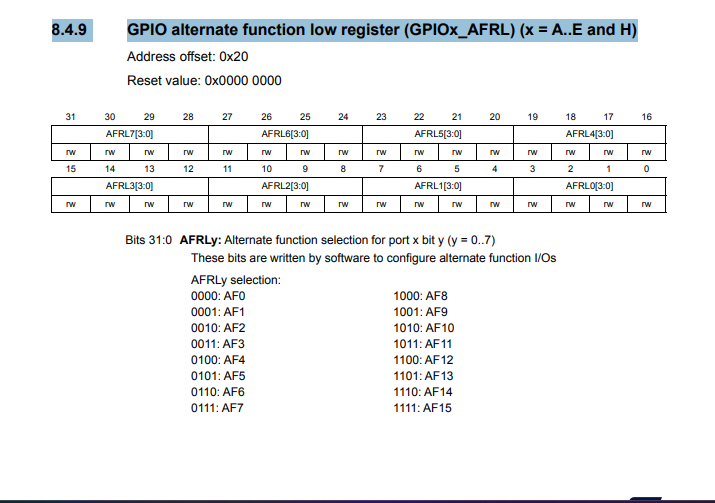
\includegraphics[width=0.8\linewidth]{imagens/GPIOx_AFRL.png}
    \caption{GPIOx\_AFRL ou GPIOx$\rightarrow$AFR[0]}
\end{figure}

A partir do momento em que o AFR e o MODER estão configurados, uma ``ponte de cobre'' virtual é fechada no silício. O TIM2 agora tem controle direto e absoluto daquele pino físico, sem nenhuma intervenção da CPU.

\vspace{0.3cm}
\noindent\textbf{2. A Anatomia dos Registradores do Timer (CCMR, CCER e CR1)}\\
Na configuração Bare-Metal, o Timer precisa ser moldado para gerar o PWM. Ele faz isso através de três registradores de controle fundamentais que ditam o comportamento de cada canal:

\textbf{O Registrador CCMR (Capture/Compare Mode Register):} É o ``Cérebro'' do canal. Cada Timer possui dois desses (CCMR1 gerencia os canais 1 e 2; CCMR2 gerencia os canais 3 e 4). Seu trabalho é definir o que o canal é e como ele se comporta. No caso do PWM (Canal 1), configuramos dois campos nele:
\begin{itemize}
    \item \textbf{Modo do Canal (CC1S):} Definimos como Saída (Output).
    \item \textbf{Modo de Comparação (OC1M):} Aqui definimos o comportamento lógico. Escrevemos o valor 110 (PWM Mode 1). Isso crava no hardware a regra: ``Deixe o pino em ALTO enquanto o cronômetro for menor que o CCR, e em BAIXO quando for maior''.
\end{itemize}

\begin{figure}[H]
    \centering
    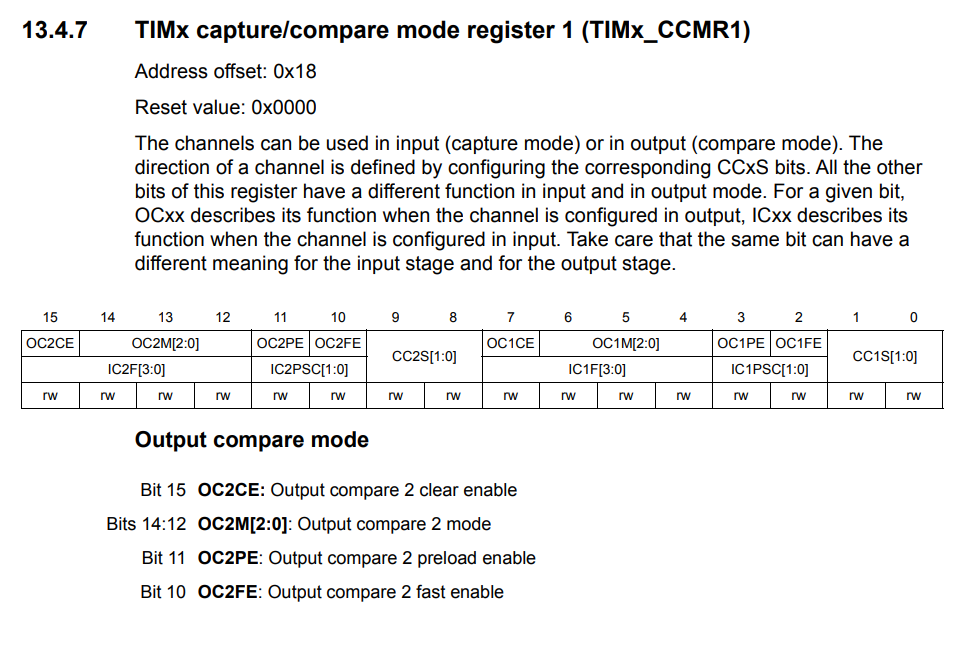
\includegraphics[width=0.8\linewidth]{imagens/TIMx_CCMR1_1.png}
    \caption{TIMx\_CCMR1\_1}
\end{figure}
\begin{figure}[H]
    \centering
    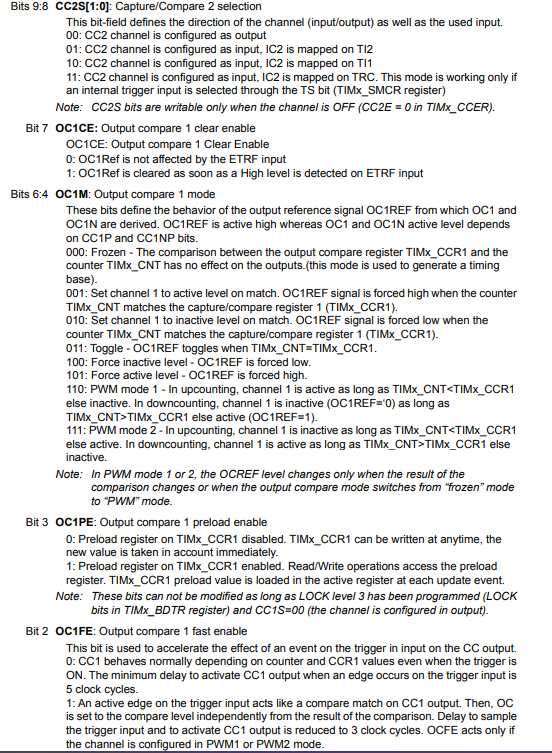
\includegraphics[width=0.8\linewidth]{imagens/TIMx_CCMR1_2.png}
    \caption{TIMx\_CCMR1\_2}
\end{figure}
\begin{figure}[H]
    \centering
    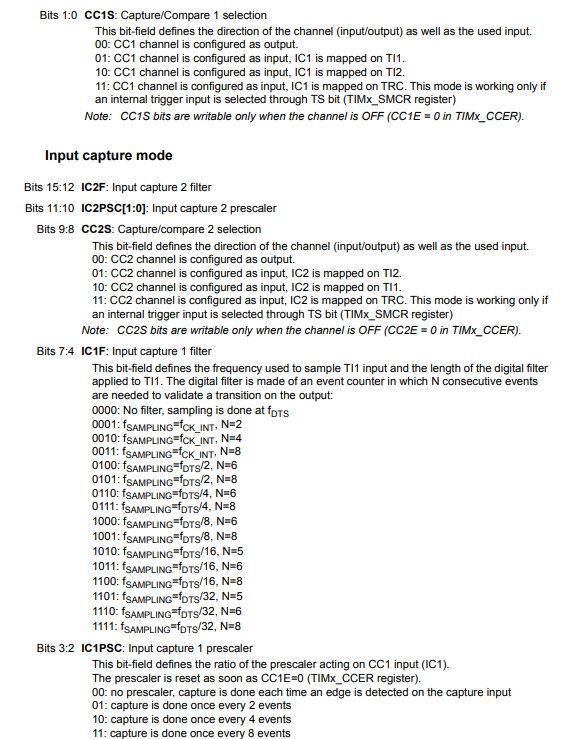
\includegraphics[width=0.8\linewidth]{imagens/TIMx_CCMR1_3.png}
    \caption{TIMx\_CCMR1\_3}
\end{figure}
\begin{figure}[H]
    \centering
    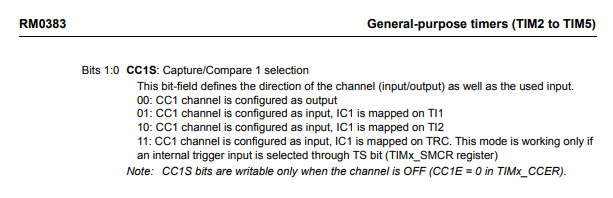
\includegraphics[width=0.8\linewidth]{imagens/TIMx_CCMR1_4.png}
    \caption{TIMx\_CCMR1\_4}
\end{figure}

\textbf{O Registrador CCER (Capture/Compare Enable Register):} É a ``Porta de Saída'' do canal. O Timer pode estar rodando internamente, o cronômetro girando e o PWM sendo gerado na lógica do chip. Mas, se você não for no registrador CCER e levantar o bit \texttt{CC1E} (Capture/Compare 1 Enable), a porta permanece trancada. O sinal não sai do Timer e não chega no multiplexador do GPIO. É o interruptor final que ativa ou corta o sinal do canal em direção ao mundo externo.

\begin{figure}[H]
    \centering
    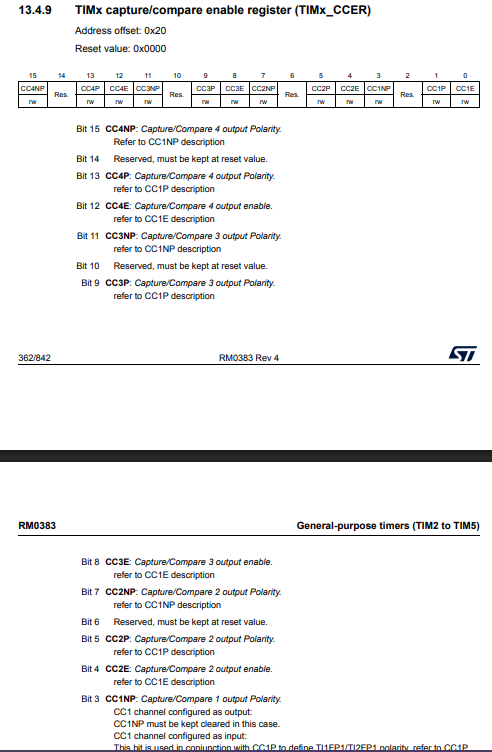
\includegraphics[width=0.8\linewidth]{imagens/TIMx_CCER1_1.png}
    \caption{TIMx\_CCER1\_1}
\end{figure}
\begin{figure}[H]
    \centering
    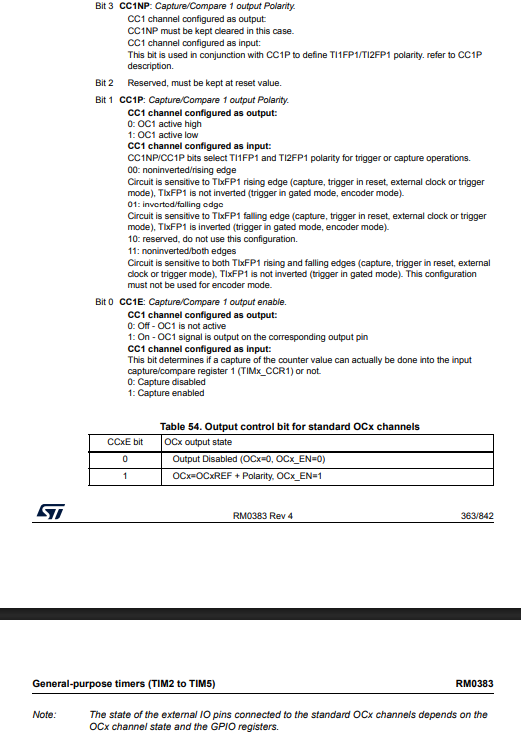
\includegraphics[width=0.8\linewidth]{imagens/TIMx_CCER1_2.png}
    \caption{TIMx\_CCER1\_2}
\end{figure}

\textbf{O Registrador CR1 (Control Register 1):} É a ``Chave de Ignição'' do motor principal do Timer. Ele controla o periférico como um todo (e não os canais individuais). Depois que você configurou o Prescaler, o ARR, o CCMR e abriu a porta no CCER, o cronômetro ainda está parado no zero. O pulso cardíaco final exige que você levante o bit \texttt{CEN} (Counter Enable) no registrador CR1. Só então o relógio começa a bater.

\vspace{0.3cm}
\noindent\textbf{Dúvida Comum: NVIC (Interrupções) vs. Canais do PWM}
\begin{enumerate}
    \item \textbf{PWM precisa de interrupção (NVIC)?} Não. A geração do PWM ocorre puramente no hardware, nos transistores de silício do Timer. Você configura o PSC, o ARR e o CCR, dá o \textit{start} e a CPU pode ir dormir. O hardware levanta e abaixa a tensão do pino automaticamente sem rodar uma única linha de código. Você só ativaria a interrupção no NVIC se precisasse que o código C fosse avisado toda vez que o ciclo reiniciasse (ex: para calcular uma malha de controle PID sincronizada com o motor), mas o PWM em si não depende disso.
    \item \textbf{Os 4 Canais são independentes? Funcionam ao mesmo tempo?} Sim e não. Um Timer (ex: TIM2) possui 1 contador (CNT), 1 Prescaler (PSC) e 1 ARR. Mas ele possui 4 canais de saída independentes, cada um com o seu próprio registrador CCR (CCR1, CCR2, CCR3, CCR4). 
    \begin{itemize}
        \item \textbf{O que isso significa fisicamente?} Todos os 4 pinos geram PWM perfeitamente ao mesmo tempo, de forma paralela pelo hardware.
        \item \textbf{O Limite:} Como todos compartilham o mesmo ARR, todos os 4 canais são obrigados a rodar na mesma \textbf{Frequência} (ex: 50 Hz).
        \item \textbf{A Independência:} Como cada um tem seu próprio CCR, cada canal pode ter um \textbf{Duty Cycle} diferente. Você pode ter o Canal 1 movendo um servo para a esquerda (CCR = 1000), o Canal 2 movendo outro para a direita (CCR = 2000) e o Canal 3 com um LED meio apagado (CCR = 500), tudo operando na mesma frequência base.
    \end{itemize}
\end{enumerate}

\vspace{0.3cm}
\noindent\textbf{3. A Diferença Essencial: EXTI vs. TIM}\\
Por fim, a confusão entre EXTI e TIM é comum porque ambos lidam com tempo e eventos, mas eles são arquiteturalmente o oposto um do outro.

\textbf{EXTI (External Interrupt / Event Controller) é Reativo e Assíncrono:}
\begin{itemize}
    \item \textbf{A Natureza:} Ele olha de dentro do chip para o mundo externo.
    \item \textbf{O Comportamento:} Ele fica completamente ocioso, esperando que algo aconteça no mundo físico de forma imprevisível (um usuário apertando um botão, um sensor de colisão fechando contato). Ele não obedece a um relógio interno; ele age imediatamente (assíncrono) assim que a borda do sinal externo muda, "gritando" para a CPU parar o que está fazendo.
\end{itemize}

\textbf{TIM (Timer) é Proativo e Síncrono:}
\begin{itemize}
    \item \textbf{A Natureza:} Ele olha do relógio interno do chip para o mundo (seja gerando sinais para fora ou medindo intervalos de forma ditatorial).
    \item \textbf{O Comportamento:} Ele é uma máquina previsível e rítmica. Ele não espera o mundo ditar as regras; ele cria o ritmo baseado no cristal oscilador da placa. Mesmo quando usado no modo Input Capture (para ler o sinal de um rádio, por exemplo), ele o faz comparando o evento com a sua própria contagem de tempo contínua e ininterrupta.
\end{itemize}

\textit{Em resumo:} O EXTI reage ao caos do mundo físico externo, enquanto o TIM impõe a ordem e a matemática do relógio interno sobre o hardware.

\subsubsection{Clock Configuration do CubeMX}
\textit{Nota: teremos uma sessão só dedicada as configurações do CubeMX ao final, esse é um detalhamento do Clock Configuration.}

Tendo compreendido o que foi passado nessa parte de Clock, a configuração deixa de ser algo tão místico. Tente observar a imagem e perceber todos os detalhes que foram explicados:

\begin{figure}[H]
    \centering
    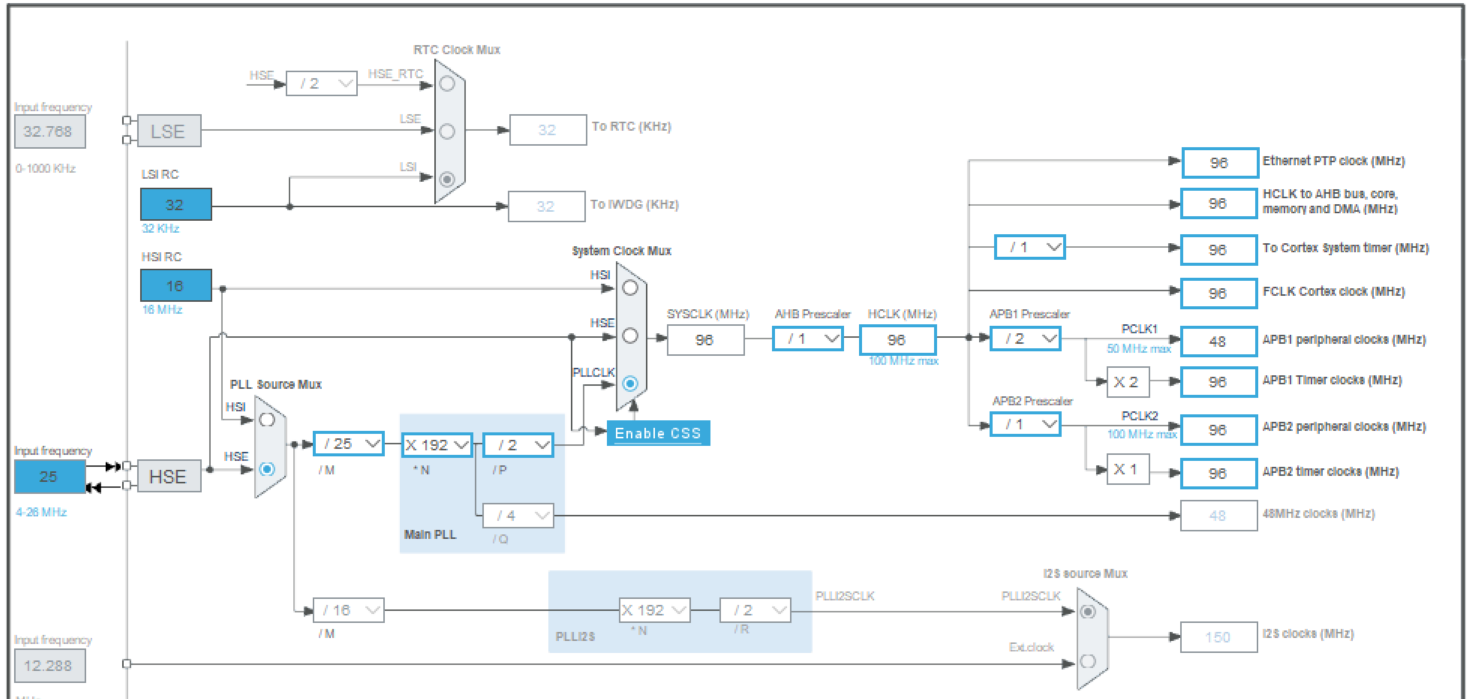
\includegraphics[width=0.8\linewidth]{imagens/Clock_CubeMX_1.png}
    \caption{Clock\_CubeMX\_1}
\end{figure}

\begin{figure}[H]
    \centering
    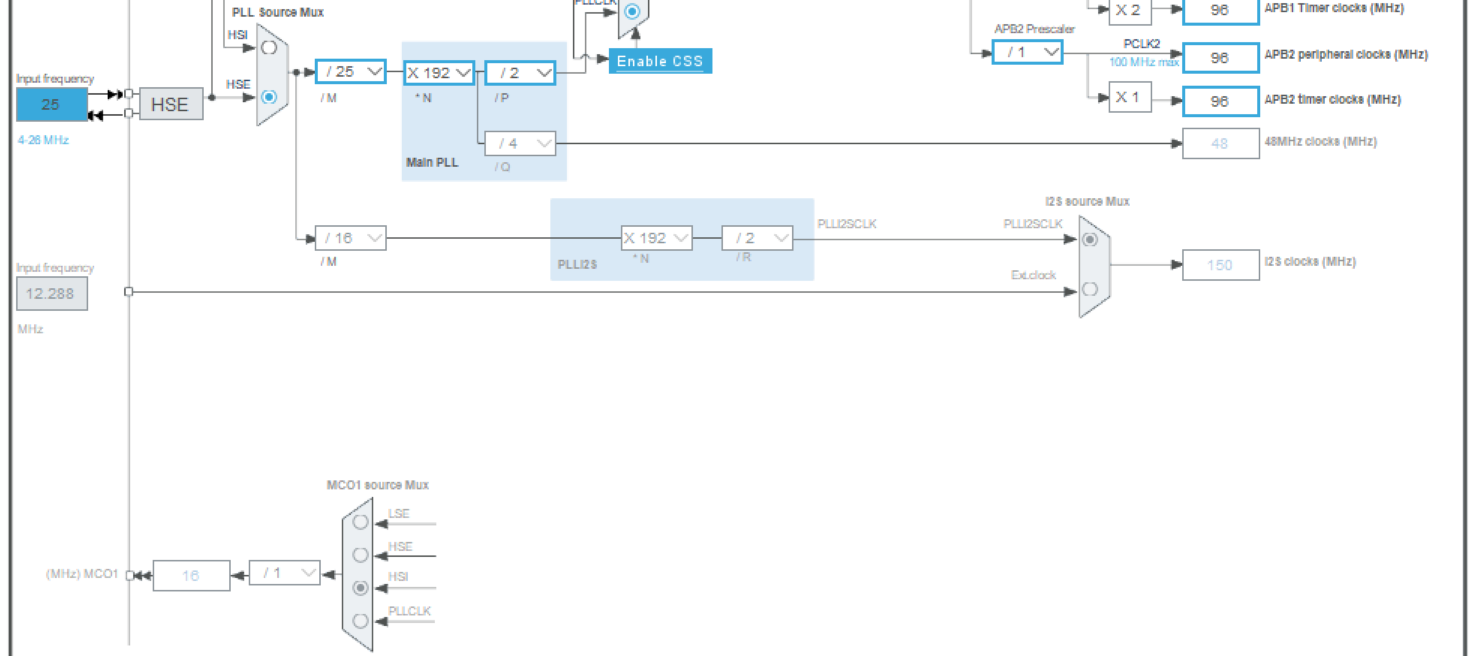
\includegraphics[width=0.8\linewidth]{imagens/Clock_CubeMX_2.png}
    \caption{Clock\_CubeMX\_2}
\end{figure}

\begin{enumerate}
    \item \textbf{O Multiplicador Oculto dos Timers (A pegadinha do APB1):} Na primeira imagem, você pode ver que o sinal passa pelo \texttt{APB1 Prescaler} configurado como / 2. Isso gera um clock de barramento (\texttt{PCLK1}) de 48 MHz. No entanto, logo abaixo, a caixa \texttt{APB1 Timer clocks} mostra impressionantes 96 MHz. Isso ocorre devido a uma regra oculta gravada no silício do STM32: Se o prescaler do barramento APB for qualquer valor diferente de / 1, o hardware aciona um multiplicador automático de X 2 especificamente para os Timers daquele barramento. Ignorar esse multiplicador é a principal causa de engenheiros calcularem o ARR e o Prescaler para gerar um PWM de 50 Hz, mas o pino acabar piscando a 100 Hz.
    \item \textbf{IWDG (Independent Watchdog) e o LSI:} Também na primeira imagem, o oscilador interno \texttt{LSI RC} (32 KHz) alimenta diretamente uma caixa chamada \texttt{To IWDG (KHz)}. Este é o \textit{Independent Watchdog}. O Watchdog é um timer de segurança vital em aviônica. Ele funciona como uma bomba-relógio: o seu código \texttt{main()} precisa reiniciá-lo constantemente. Se o seu código travar em um loop infinito ou sofrer interferência eletromagnética, ele para de ``alimentar o cão''. Quando o timer do IWDG zera, ele força um reset físico no microcontrolador. Como ele é alimentado por esse oscilador LSI dedicado, ele funciona mesmo se o cristal principal (HSE) explodir no voo.
    \item \textbf{MCO1 (A Saída de Clock para Debug):} Na segunda imagem, no canto inferior, existe um multiplexador chamado \texttt{MCO1 source Mux} apontando para um pino físico. MCO significa \textit{Microcontroller Clock Output}. Essa ferramenta permite que você pegue um sinal interno (como o HSI, HSE ou o próprio PLL) e jogue direto para um pino GPIO externo (geralmente o PA8). É extremamente útil na bancada: você conecta um osciloscópio nesse pino para provar fisicamente se o seu cristal externo de 25 MHz está oscilando na frequência correta ou se tem muito ruído.
    \item \textbf{A Matemática da ``Caixa de Marchas'' (Main PLL):} A primeira imagem destrincha as entranhas do \textit{Main PLL}. O PLL (Phase-Locked Loop) pega a frequência de entrada de 25 MHz e passa por três estágios:
    \begin{itemize}
        \item \textbf{/ M:} Um divisor inicial (na imagem, 25) para baixar e estabilizar a frequência.
        \item \textbf{X N:} Um super-multiplicador (na imagem, 192) que joga a frequência lá para cima.
        \item \textbf{/ P e / Q:} Divisores finais. O \texttt{/ P} (configurado como 2) dita a velocidade do processador \texttt{SYSCLK} (96 MHz). O \texttt{/ Q} (configurado como 4) é uma saída separada exigida por hardwares rigorosos que precisam de exatamente 48 MHz para funcionar, como a porta USB.
    \end{itemize}
    \item \textbf{Resumo: O RTC e o Cristal LSE:} Vemos no diagrama superior que o pino LSE recebe exatos 32.768 KHz e alimenta o bloco \texttt{RTC Clock Mux}. (\textit{Nota: A explicação completa da inicialização em Bare-Metal, formato BCD e registradores do Real-Time Clock está no \hyperref[anexo:9]{Anexo 9} do material}). Em suma, o RTC é o relógio/calendário isolado do sistema. Diferente dos Timers convencionais que perdem a memória quando a placa é desligada, o RTC possui um domínio de energia próprio (Vbat). Esse oscilador LSE de baixíssimo consumo continua batendo perfeitamente, garantindo que os logs de telemetria do foguete continuem com dia e hora corretos, mesmo após um reset total do processador principal.
    \item \textbf{O Salva-Vidas do Hardware: CSS (Clock Security System):} Bem no centro do diagrama principal, conectado ao multiplexador do sistema, existe um botão azul escrito \texttt{Enable CSS}. O CSS é um circuito de segurança vital em engenharia aeroespacial. Quando você usa um cristal externo (HSE) para guiar o chip, existe o risco físico de a solda quebrar devido a vibrações de alta frequência no voo. Se o cristal parar, o chip morreria. Ao ativar o CSS, o hardware fica monitorando o pino do HSE. Se ele detectar que a oscilação parou, o STM32 automaticamente e via hardware desconecta o cristal quebrado, liga o oscilador interno de emergência (HSI a 16 MHz) e dispara uma Interrupção Não Mascarável (NMI). Isso salva o processador do travamento e dá tempo ao seu código para registrar a falha e iniciar um protocolo de aborto ou redundância.
    \item \textbf{A Dissecção do Núcleo (AHB, SysTick e FCLK):} No detalhe superior direito do diagrama, vemos um barramento rodando a 96 MHz se dividindo em quatro subsistemas essenciais para o funcionamento interno:
    \begin{itemize}
        \item \textbf{HCLK to AHB bus, core, memory and DMA:} Este é o coração do chip. O AHB (Advanced High-performance Bus) é a rodovia principal que conecta o processador à memória RAM, à memória Flash e ao controlador de acesso direto à memória (DMA). É a velocidade ``real'' em que o processador mastiga as instruções.
        \item \textbf{To Cortex System timer:} O núcleo ARM possui um timer privado, embutido nele, chamado SysTick. Ele não é usado para gerar PWM ou ler sensores. Ele é o ``metrônomo'' do sistema operacional (como o FreeRTOS) ou a base de tempo matemática que faz a função \texttt{HAL\_Delay()} funcionar.
        \item \textbf{FCLK Cortex clock:} É um relógio de ``corrida livre'' (\textit{Free-Running Clock}) específico do processador ARM. Ele é usado exclusivamente para garantir que a CPU consiga escutar pedidos de interrupção (NVIC) e fazer depuração (via SWD), mesmo se a via principal do AHB estiver em modo de baixo consumo (Sleep).
        \item \textbf{Ethernet PTP clock:} Refere-se ao Precision Time Protocol usado em redes Ethernet. (No caso do F411, como ele não tem MAC Ethernet físico, esse relógio é um vestígio arquitetural da família STM32F4 na interface do CubeMX).
    \end{itemize}
    \item \textbf{PLLI2S e a Via Exclusiva para Áudio:} No detalhe inferior do diagrama, notamos um segundo PLL inteiro (\texttt{PLLI2S}) configurado para multiplicar o clock de entrada e gerar 150 MHz para o \texttt{I2S clocks (MHz)}. I2S (\textit{Inter-IC Sound}) é um protocolo feito estritamente para Áudio Digital (como microfones digitais ou conversores de áudio). O áudio não perdoa relógios imprecisos: para você ter um som limpo em 44.1 kHz (qualidade de CD), a frequência não pode derivar um Hz sequer. Como o PLL principal está focado em gerar frequências redondas para a CPU e para o USB (48 MHz), a ST colocou um segundo motor multiplicador exclusivo para o I2S, garantindo que o áudio tenha uma base de tempo perfeita sem interferir na matemática do processador central.
    \item \textbf{Por que o CubeMX bloqueia (deixa cinza) essas caixas?:} Ao tentar alterar o multiplicador do I2S, o MCO1 ou o LSE/LSI, você notou que eles não respondem a cliques. Essa é uma trava de proteção (e frustração comum) da interface gráfica. O CubeMX opera com a filosofia ``Pino Físico Primeiro''. Ele não deixa você ligar o relógio de algo se o hardware externo não estiver eletricamente mapeado na placa.
    \begin{itemize}
        \item \textbf{LSE/HSE Cinzas:} Só são liberados se você for na aba \textit{Pinout \& Configuration -> System Core -> RCC} e ativar fisicamente o modo \textit{Crystal/Ceramic Resonator}.
        \item \textbf{MCO1 Cinza:} Para ligar a saída de clock de diagnóstico, você precisa ir no RCC e marcar a caixa \textit{Master Clock Output 1}. Isso alocará o pino PA8 automaticamente, acendendo o multiplexador na aba de Clock.
        \item \textbf{I2S Cinza:} Só ganha cor se você ativar um periférico SPI no modo I2S Half-Duplex.
    \end{itemize}
    \item \textbf{O RTC e o Cristal Externo (Resumo):} (\textit{Nota: A configuração dos registradores e o formato BCD do Relógio de Tempo Real estão profundamente mapeados no \hyperref[anexo:9]{Anexo 9} do manual}). Na árvore de clock, vemos a caixa LSE recebendo uma frequência de exatos 32.768 KHz. Esse é o quartzo responsável por alimentar o RTC de forma independente. Como vimos no anexo, o RTC opera em seu próprio domínio de energia (Vbat). A árvore do CubeMX mostra esse circuito separado para reforçar visualmente que a contagem do calendário e das horas continua inabalável mesmo quando todos os multiplicadores principais (PLLs) e a CPU principal estão completamente desligados ou passam por um reset total de sistema.
\end{enumerate}

% ==========================================
% ADC (Analog-to-Digital Converter)
% ==========================================
\subsection{ADC (Analog-to-Digital Converter)}

Enquanto o PWM resolve o problema de criar uma saída ``analógica'' a partir de pinos digitais, o ADC (Conversor Analógico-Digital) faz o caminho inverso: ele permite que o microcontrolador ``leia'' tensões contínuas do mundo real.

Se você precisa ler a posição de um potenciômetro, a temperatura de um sensor analógico (como o LM35) ou a voltagem da bateria do seu sistema para evitar que ela descarregue demais, você obrigatoriamente passará pelo ADC.

\begin{figure}[H]
    \centering
    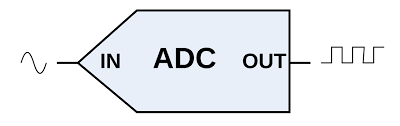
\includegraphics[width=0.8\linewidth]{imagens/ADC.png}
    \caption{ADC}
    \label{fig:adc}
\end{figure}

\subsubsection{A Matemática da Conversão (Resolução)}
O ADC do STM32 (como o do F411) possui uma resolução de 12 bits. O que isso significa na prática?
Significa que ele pega a faixa de tensão de referência (geralmente de 0V a 3.3V) e a divide em $2^{12}$ pedaços iguais, ou seja, 4096 ``degraus'' (variando de 0 a 4095).
\begin{itemize}
    \item Se o pino estiver recebendo 0V, o ADC lerá o valor 0.
    \item Se o pino estiver recebendo 3.3V, o ADC lerá o valor 4095.
    \item Se o pino estiver recebendo 1.65V (metade), o ADC lerá 2047.
\end{itemize}

A fórmula para transformar o número ``cru'' (\textit{raw}) lido do registrador em uma voltagem real na sua variável float é:
\[ V_{in} = \left( \frac{Valor\_ADC}{4095} \right) \times 3.3 \]

\subsubsection{O Capacitor de Amostragem (O Erro Invisível)}
Antes de ver o código, você precisa entender como o hardware lê a tensão. Dentro do chip, o ADC possui um pequeno capacitor e uma chave (um transistor).



Quando você manda o ADC ler um pino, ele fecha a chave e liga o pino a esse capacitor interno. O capacitor precisa de um tempo mínimo (medido em ciclos de clock) para se carregar até atingir a exata mesma tensão do mundo externo. Isso se chama \textit{Sampling Time} (Tempo de Amostragem).

\textbf{Aviso de Hardware:} Um erro clássico é configurar o ADC com um \textit{Sampling Time} muito rápido (ex: 3 ciclos). Se o seu sensor externo tiver uma impedância alta (resistência), o capacitor não terá tempo de carregar completamente, e a sua leitura no software será um valor menor do que a tensão real, flutuando aleatoriamente. Se não precisa de velocidade extrema, sempre configure o \textit{Sampling Time} para valores mais altos (ex: 84 ciclos ou 480 ciclos).

\subsubsection{ADC com HAL (O Método Polling)}
A biblioteca HAL simplifica bastante o processo, escondendo o acionamento dos clocks internos e calibrações. O método mais simples (porém bloqueante) é o Polling.

No CubeMX, você configura o pino (ex: PA0) como \texttt{ADC1\_IN0}. No \texttt{main.c}, o uso se resume a iniciar a conversão, esperar ela terminar e ler o resultado.

\begin{lstlisting}[language=C]
uint32_t adc_raw_value = 0;
float voltage = 0.0f;

/* No loop principal */
while (1)
{
  /* 1. Manda o hardware iniciar a conversao do canal configurado */
  HAL_ADC_Start(&hadc1);
  
  /* 2. Trava a CPU esperando a conversao terminar (Timeout de 1ms) */
  /* Isso e Polling: A CPU fica inutil ate o hardware responder */
  if (HAL_ADC_PollForConversion(&hadc1, 1) == HAL_OK)
  {
    /* 3. Le o valor do registrador (de 0 a 4095) */
    adc_raw_value = HAL_ADC_GetValue(&hadc1);
    
    /* 4. Converte para Volts */
    voltage = ((float)adc_raw_value / 4095.0f) * 3.3f;
  }
  
  /* Desliga o ADC para economizar energia (opcional) */
  HAL_ADC_Stop(&hadc1);
  
  HAL_Delay(100);
}
\end{lstlisting}

\textbf{Nota:} Em sistemas complexos com múltiplos sensores, o método Polling trava muito a CPU. Na indústria, usa-se o ADC engatilhado por um Timer e transferindo os dados via DMA (\textit{Direct Memory Access}), onde o hardware salva os valores do ADC direto nas suas variáveis na RAM sem a CPU precisar intervir.

\subsubsection{ADC no ``Bare-Metal'' (Lendo o Registrador DR)}
Configurar o ADC diretamente nos registradores exige ligar o pino em modo analógico, ligar o conversor e verificar a flag \texttt{EOC} (\textit{End of Conversion}) no registrador de status (\texttt{SR}). 

Vamos configurar o Canal 0 (Pino PA0):

\begin{lstlisting}[language=C]
uint32_t adc_raw_value = 0;

/* ========================================================== */
/* SETUP INICIAL (Fora do while)                              */
/* ========================================================== */

/* 1. Habilita os Clocks (GPIOA e ADC1) */
RCC->AHB1ENR |= (1UL << 0);       // Clock do GPIOA
RCC->APB2ENR |= (1UL << 8);       // Clock do ADC1 (ADC1EN)

/* 2. Configura o pino PA0 para Modo Analogico (11) no MODER */
/* Essencial: Desliga os resistores internos (Pull-Up/Down) do pino */
GPIOA->MODER |= (3UL << 0);       // Seta os bits 0 e 1 para 11 (Analog Mode)
GPIOA->PUPDR &= ~(3UL << 0);      // Limpa os bits de Pull

/* 3. Configura o ADC (Sampling Time e Sequencia) */
/* SMPR2: Configura o tempo de amostragem do Canal 0 (ex: 84 ciclos) */
ADC1->SMPR2 |= (4UL << 0);        // 100: 84 cycles no canal 0

/* SQR3: Define qual canal sera lido na primeira conversao da sequencia */
ADC1->SQR3 &= ~(0x1FUL << 0);     // Limpa os primeiros 5 bits e deixa em 0 (Canal 0)

/* 4. Liga a energia do ADC (ADON) */
ADC1->CR2 |= (1UL << 0);          // ADON (A/D Converter ON)

/* ========================================================== */
/* NO LOOP PRINCIPAL                                          */
/* ========================================================== */
while (1)
{
  /* 1. Inicia a conversao (SWSTART - Start Conversion of regular channels) */
  ADC1->CR2 |= (1UL << 30);
  
  /* 2. Aguarda a flag EOC (End Of Conversion) no Status Register (Polling) */
  /* Enquanto o bit 1 (EOC) for 0, o loop fica travado aqui */
  while (!(ADC1->SR & (1UL << 1)));
  
  /* 3. Le o Data Register (A leitura do DR automaticamente limpa a flag EOC) */
  adc_raw_value = ADC1->DR;
  
  /* (Opcional) Seu delay rustico aqui */
}
\end{lstlisting}

\textbf{A Mágica da Limpeza da Flag:} No Bare-Metal, diferentemente da interrupção do EXTI (onde você é obrigado a escrever ``1'' na flag de Pending para limpá-la), a engenharia do STM32 simplificou o ADC. O ato físico da CPU acessar e ler o endereço do registrador \texttt{ADC1->DR} aciona um circuito interno que limpa a flag \texttt{EOC} instantaneamente.

Aqui estão os registradores (\texttt{SMPR2} e \texttt{SQR3} serão melhor explicados em sequência):

\begin{figure}[H]
    \centering
    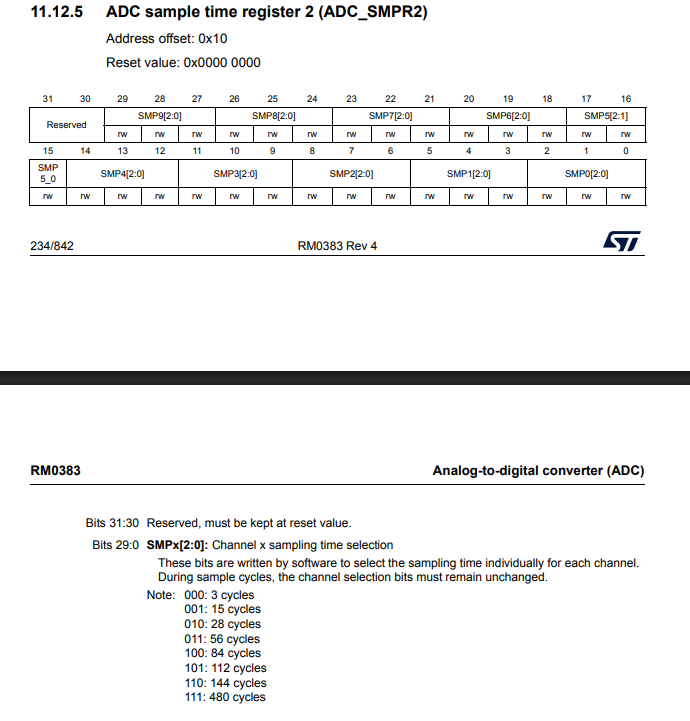
\includegraphics[width=0.8\linewidth]{imagens/ADC_SMPR2.png}
    \caption{ADC\_SMPR2}
\end{figure}
\begin{figure}[H]
    \centering
    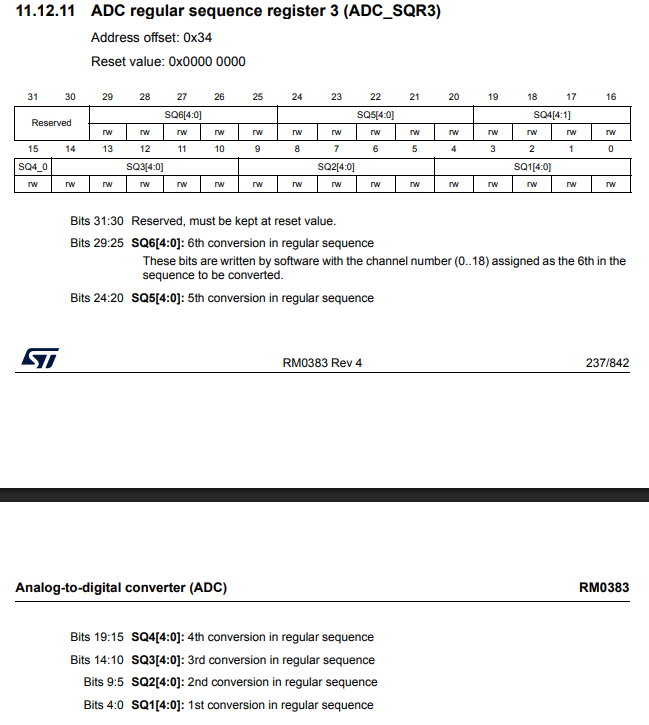
\includegraphics[width=0.8\linewidth]{imagens/ADC_SQR3.png}
    \caption{ADC\_SQR3}
\end{figure}
\begin{figure}[H]
    \centering
    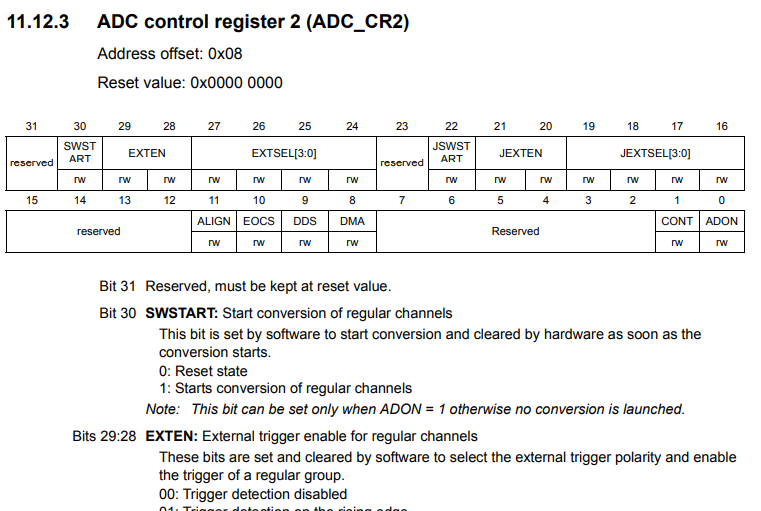
\includegraphics[width=0.8\linewidth]{imagens/ADC_CR2_1.png}
    \caption{ADC\_CR2\_1}
\end{figure}
\begin{figure}[H]
    \centering
    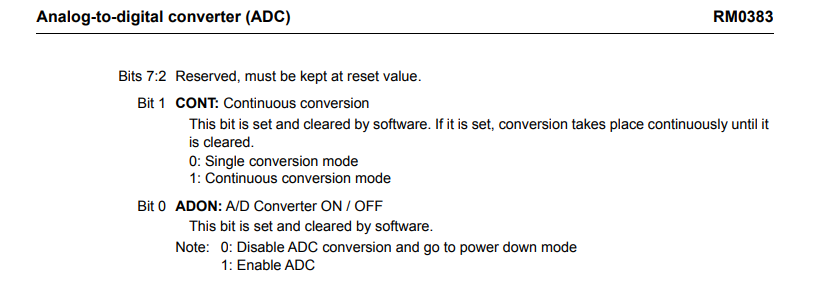
\includegraphics[width=0.8\linewidth]{imagens/ADC_CR2_2.png}
    \caption{ADC\_CR2\_2}
\end{figure}
\begin{figure}[H]
    \centering
    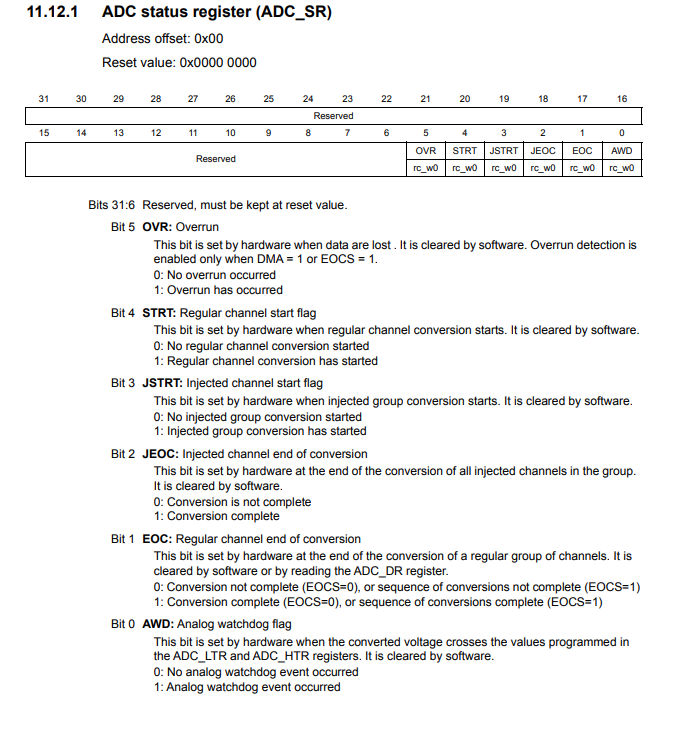
\includegraphics[width=0.8\linewidth]{imagens/ADC_SR.png}
    \caption{ADC\_SR}
\end{figure}
\begin{figure}[H]
    \centering
    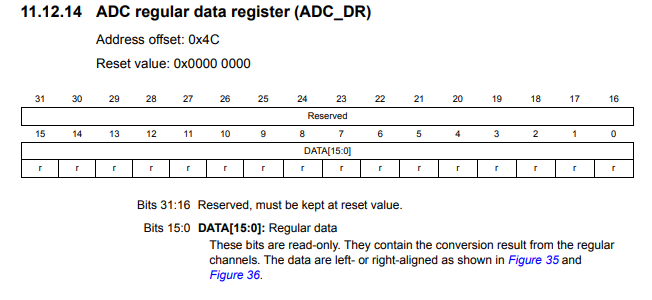
\includegraphics[width=0.8\linewidth]{imagens/ADC_DR.png}
    \caption{ADC\_DR}
\end{figure}

\subsubsection{O que são os Canais do ADC?}
O STM32F411 não possui 16 ADCs independentes lá dentro. Ele possui um \textbf{único motor conversor ADC} (o circuito físico que faz a matemática de tensões).



No entanto, a ST colocou um Multiplexador (uma chave seletora) na entrada desse motor. Essa chave consegue conectar o motor a 16 pinos físicos diferentes do microcontrolador. Cada uma dessas conexões possíveis é chamada de \textbf{Canal}.
\begin{itemize}
    \item O pino PA0 está fisicamente ligado ao Canal 0.
    \item O pino PA1 está ligado ao Canal 1.
    \item O pino PB0 está ligado ao Canal 8, e assim por diante.
\end{itemize}

Isso significa que o ADC só consegue ler um pino por vez. Se você precisa ler 3 sensores (ex: Eixo X, Y e Z de um acelerômetro analógico), você precisa mandar o ADC ler o Canal 0, terminar, mudar a chave para o Canal 1, ler, terminar, e mudar a chave para o Canal 2. É aqui que entram os registradores numerados!

\subsubsection{Desmistificando os Registradores (Por que SMPR2 e SQR3?)}
A arquitetura ARM é de 32 bits, o que significa que as ``gavetas'' (registradores) têm no máximo 32 espaços (bits) de largura. Quando a ST foi criar os registradores de configuração do ADC, as informações simplesmente não couberam em um registrador só.

\vspace{0.3cm}
\noindent\textbf{1. A Família SMPR (Sample Time Register)}\\
O hardware permite que você configure um ``Tempo de Amostragem'' diferente para cada um dos 16 canais. Ele exige 3 bits para configurar um único canal.
Se multiplicarmos 3 bits por 16 canais, precisamos de 48 bits. Como o registrador só tem 32 bits, a ST foi obrigada a dividi-lo em dois:
\begin{itemize}
    \item \textbf{SMPR2:} Configura o tempo de amostragem dos Canais de 0 a 9 (ocupa 30 bits).
    \item \textbf{SMPR1:} Configura o tempo de amostragem dos Canais de 10 a 18 (incluindo sensores internos de temperatura).
\end{itemize}
É por isso que no código Bare-Metal anterior configuramos o PA0 (Canal 0) mexendo no \texttt{SMPR2}.

\vspace{0.3cm}
\noindent\textbf{2. A Família SQR (Regular Sequence Register)}\\
Se você quer ler vários sensores em sequência automática, o ADC precisa de uma ``Lista de Tarefas'' dizendo quem ele lê primeiro, quem lê em segundo, etc.
Cada posição na lista precisa de 5 bits para indicar o número do canal. Novamente, não cabe tudo em 32 bits. A ST criou três registradores para guardar essa lista:
\begin{itemize}
    \item \textbf{SQR3:} Guarda qual canal será lido na 1ª, 2ª, 3ª, 4ª, 5ª e 6ª posição da fila.
    \item \textbf{SQR2:} Guarda da 7ª à 12ª posição.
    \item \textbf{SQR1:} Guarda da 13ª à 16ª posição. Além disso, os últimos bits do SQR1 definem o ``Tamanho Total da Fila'' (ex: ``Leia 3 canais e pare'').
\end{itemize}
No nosso código básico, limpamos os primeiros bits do \texttt{SQR3} para colocar o Canal 0 na primeira posição da fila.

\subsubsection{A Arquitetura Profissional: ADC acionado por Timer + DMA}
O método Polling (travar a CPU no while esperando o ADC terminar) é amador. Em sistemas de aviônica ou controle, a CPU tem coisas mais importantes para fazer (como calcular matrizes e malhas PID).

A solução de engenharia para isso é criar um \textbf{``Efeito Dominó'' em Hardware}:
\begin{enumerate}
    \item Você configura um Timer (ex: TIM3) para estourar a exatos 100 Hz. Mas o Timer \textbf{não vai gerar interrupção para a CPU}; o pino de saída interno dele (\texttt{TRGO}) vai cutucar fisicamente o ADC.
    \item O ADC recebe o cutucão do Timer, acorda, lê o sensor (ou a sequência de sensores) e, quando termina, gera um pulso avisando o DMA.
    \item O DMA (\textit{Direct Memory Access}), que é um controlador de transferência independente, vai até o registrador \texttt{ADC1->DR}, pega o valor lido e copia silenciosamente para a sua variável na memória RAM.
\end{enumerate}

\textbf{Resultado:} A CPU nunca trava. Você simplesmente acessa a sua variável na RAM quando quiser, e o valor lá dentro estará sendo magicamente atualizado 100 vezes por segundo pelo hardware de fundo.

\vspace{0.3cm}
\noindent\textbf{Como fazer isso com a HAL?}\\
No CubeMX, você ativa o Timer, ativa o ADC configurando o \textit{External Trigger Conversion Source} para o evento do Timer, e na aba ``DMA Settings'' do ADC, adiciona o canal do DMA no modo Circular. O código gerado fará todo o setup. No \texttt{main.c}, você só escreve duas linhas antes do \texttt{while(1)}:

\begin{lstlisting}[language=C]
uint16_t buffer_sensores[3]; // Variavel na RAM para guardar os valores

/* 1. Liga o Timer base para bater no ritmo desejado */
HAL_TIM_Base_Start(&htim3);

/* 2. Liga o ADC atrelado ao DMA informando o endereco da variavel */
HAL_ADC_Start_DMA(&hadc1, (uint32_t*)buffer_sensores, 3);

while(1) {
  /* A CPU fica 100% livre. O buffer_sensores[0], [1] e [2] 
     sao atualizados automaticamente pelo hardware! */
}
\end{lstlisting}

\textbf{Outro exemplo:}\\
Na abordagem com HAL, assumimos que as funções \texttt{MX\_...\_Init()} foram geradas pelo CubeMX no final do arquivo. O seu trabalho real se concentra na inicialização do fluxo antes do laço principal.

\begin{lstlisting}[language=C]
#include "main.h"

/* Variaveis exportadas pelo CubeMX */
ADC_HandleTypeDef hadc1;
DMA_HandleTypeDef hdma_adc1;
TIM_HandleTypeDef htim3;

/* Buffer na RAM para guardar as leituras do ADC */
/* Tamanho 1 pois estamos lendo apenas o Canal 0 neste exemplo */
uint16_t adc_buffer[1]; 

void SystemClock_Config(void);
static void MX_GPIO_Init(void);
static void MX_DMA_Init(void);
static void MX_ADC1_Init(void);
static void MX_TIM3_Init(void);

int main(void)
{
  /* 1. Inicializa a biblioteca HAL e o Clock do Sistema */
  HAL_Init();
  SystemClock_Config();

  /* 2. Inicializa os perifericos (Hardware gerado pelo CubeMX) */
  MX_GPIO_Init();
  MX_DMA_Init();   /* O DMA DEVE ser inicializado antes do ADC */
  MX_ADC1_Init();
  MX_TIM3_Init();

  /* ========================================================== */
  /* 3. LIGA O SISTEMA EM CADEIA (Efeito Domino)                */
  /* ========================================================== */
  
  /* Liga o Timer 3, que vai gerar os pulsos (TRGO) na frequencia configurada */
  HAL_TIM_Base_Start(&htim3);

  /* Liga o ADC no modo DMA. 
     Ele fica aguardando o pulso do Timer 3 para ler e o DMA transfere para adc_buffer */
  HAL_ADC_Start_DMA(&hadc1, (uint32_t*)adc_buffer, 1);

  /* ========================================================== */
  while (1)
  {
    /* A CPU fica 100% livre aqui.
       O valor de adc_buffer[0] estara sempre atualizado com a ultima 
       leitura real do sensor, feita em background pelo hardware. */
       
    // Exemplo de uso:
    // float tensao = (adc_buffer[0] / 4095.0f) * 3.3f;
    // HAL_Delay(500); 
  }
}
\end{lstlisting}

\vspace{0.3cm}
\noindent\textbf{Como funciona no Bare-Metal (A Dança dos Registradores)}\\
No Bare-Metal, precisamos amarrar esses três periféricos ``no osso''. O código é um pouco mais denso, mas revela exatamente os caminhos do silício. Suponha que queremos ler apenas o Canal 0 (PA0) engatilhado pelo TIM3:

\begin{lstlisting}[language=C]
/* Buffer na RAM para guardar a leitura do ADC */
volatile uint16_t adc_buffer[1];

/* ========================================================== */
/* 1. CONFIGURACAO DO DMA2 (Fluxo: ADC -> RAM)                */
/* ========================================================== */
RCC->AHB1ENR |= (1UL << 22); // Liga o Clock do DMA2

/* Configura o Stream 0 do DMA2 (que atende o ADC1) */
DMA2_Stream0->CR &= ~DMA_SxCR_EN; // Desliga o DMA para configurar

/* Define os enderecos da entrega */
DMA2_Stream0->PAR = (uint32_t)&ADC1->DR;      // Origem: Registrador de Dados do ADC
DMA2_Stream0->M0AR = (uint32_t)&valor_sensor; // Destino: Nossa variavel na RAM
DMA2_Stream0->NDTR = 1;                       // Quantidade de dados a transferir

/* Configura o comportamento do DMA (Circular, 16 bits de tamanho) */
DMA2_Stream0->CR |= (1UL << 8);  // CIRC: Modo Circular (nunca para de transferir)
DMA2_Stream0->CR |= (1UL << 11); // PSIZE: Tamanho da origem 16-bits (Half-Word)
DMA2_Stream0->CR |= (1UL << 13); // MSIZE: Tamanho do destino 16-bits
DMA2_Stream0->CR |= (1UL << 0);  // EN: Liga o DMA

/* ========================================================== */
/* 2. CONFIGURACAO DO ADC (Para ouvir o Timer e usar o DMA)   */
/* ========================================================== */
/* (Assumindo que Clocks e GPIO ja estao configurados) */
ADC1->CR2 |= (1UL << 8);  // DMA: Habilita o ADC para mandar requisicoes ao DMA
ADC1->CR2 |= (1UL << 9);  // DDS: DMA continua mandando requisicoes mesmo apos a 1a rodada

/* Configura o Gatilho Externo (Timer 3 TRGO) */
ADC1->CR2 |= (1UL << 28); // EXTEN: Gatilho ativo na borda de subida (Rising Edge)
ADC1->CR2 |= (8UL << 24); // EXTSEL: Seleciona o Evento 8 (Timer 3 TRGO no F411)

ADC1->CR2 |= (1UL << 0);  // ADON: Liga o ADC

/* ========================================================== */
/* 3. CONFIGURACAO DO TIM3 (O Metronomo)                      */
/* ========================================================== */
RCC->APB1ENR |= (1UL << 1); // Clock do TIM3
TIM3->PSC = 8400 - 1;       // Prescaler
TIM3->ARR = 100 - 1;        // ARR definindo a frequencia

/* Configura o pino de saida interno (TRGO) para pulsar a cada Update (quando zera) */
TIM3->CR2 |= (2UL << 4);    // MMS: 010 (Update event atua como TRGO)

TIM3->CR1 |= (1UL << 0);    // CEN: Liga o Timer! O efeito domino comeca aqui.
\end{lstlisting}

Os registradores do DMA são esses:

\begin{figure}[H]
    \centering
    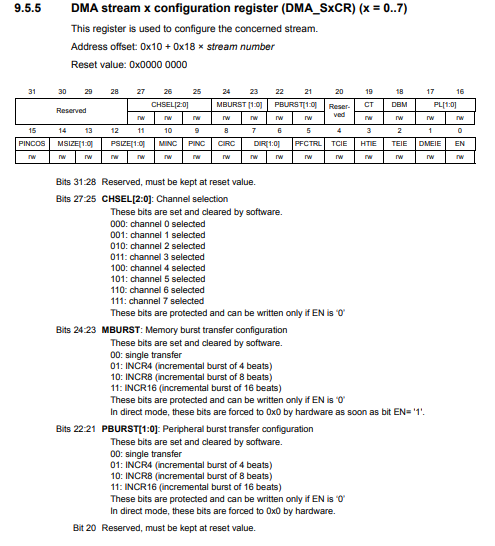
\includegraphics[width=0.8\linewidth]{imagens/DMA_SxCR.png}
    \caption{DMA\_SxCR}
\end{figure}
\begin{figure}[H]
    \centering
    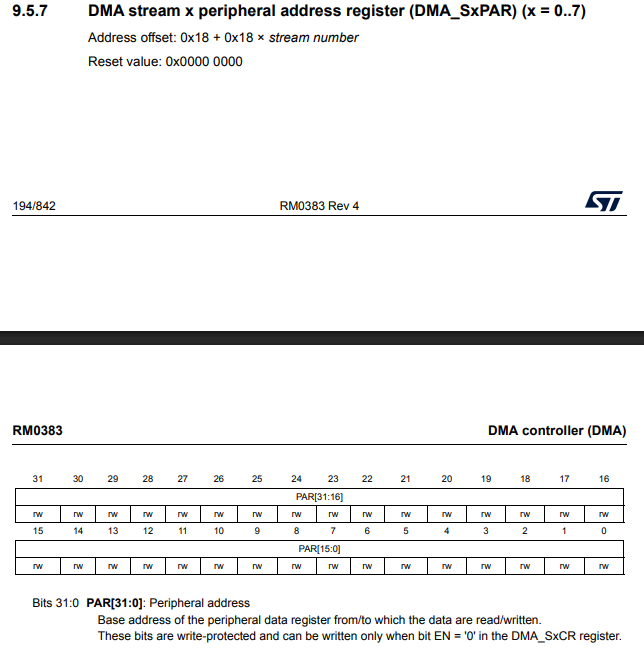
\includegraphics[width=0.8\linewidth]{imagens/DMA_PAR.png}
    \caption{DMA\_PAR}
\end{figure}
\begin{figure}[H]
    \centering
    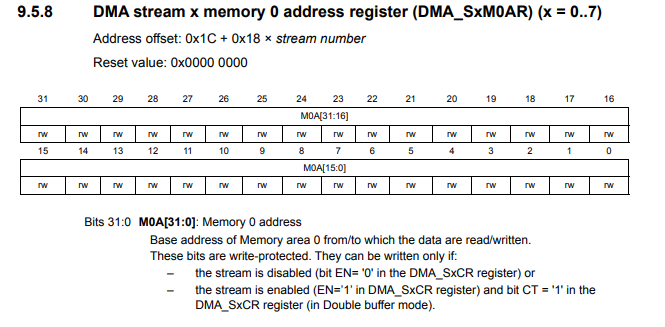
\includegraphics[width=0.8\linewidth]{imagens/DMA_SxM0AR.png}
    \caption{DMA\_SxM0AR}
\end{figure}
\begin{figure}[H]
    \centering
    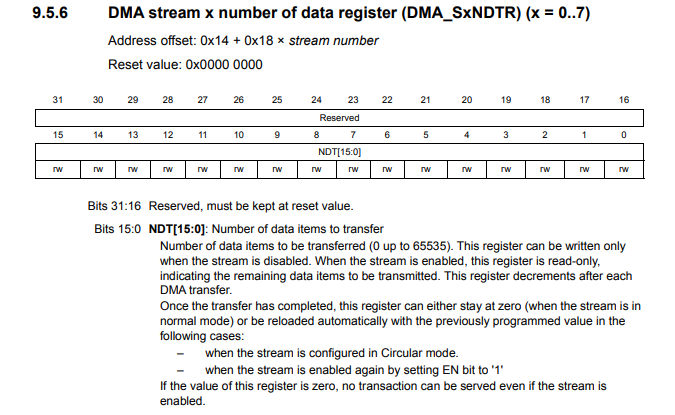
\includegraphics[width=0.8\linewidth]{imagens/DMA_SxNDTR.png}
    \caption{DMA\_SxNDTR}
\end{figure}

% ==========================================
% UART (Universal Asynchronous Receiver/Transmitter)
% ==========================================
\subsection{UART (Universal Asynchronous Receiver/Transmitter)}

\begin{figure}[H]
    \centering
    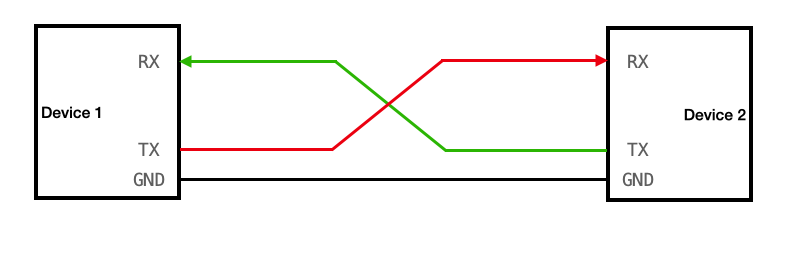
\includegraphics[width=0.8\linewidth]{imagens/UART.png}
    \caption{UART}
    \label{fig:uart}
\end{figure}

Diferente do barramento interno (AHB/APB) que movimenta 32 bits de uma vez em paralelo, a comunicação serial movimenta os dados em ``fila indiana'' (um bit atrás do outro) através de um único fio.

A principal característica da UART está no ``A'' da sigla: \textbf{Assíncrona}. Isso significa que não existe um fio de Clock conectando os dois dispositivos para ditar o ritmo da conversa. Para que eles se entendam, ambos precisam concordar previamente com a exata mesma velocidade de transmissão.

\subsubsection{Serial Communication (A Teoria)}
Para conectar dois dispositivos via UART, você precisa de apenas três fios:
\begin{itemize}
    \item \textbf{TX (Transmit):} O pino que fala.
    \item \textbf{RX (Receive):} O pino que escuta.
    \item \textbf{GND (Terra):} A referência elétrica comum (Obrigatório! Sem ele, as voltagens não têm referência e a comunicação falha).
\end{itemize}
\textbf{Regra de ouro:} A conexão é sempre cruzada. O TX do Microcontrolador liga no RX do Sensor (ou do PC), e vice-versa.

\vspace{0.3cm}
\noindent\textbf{O Pacote de Dados (Frame):}\\
Como não há clock contínuo para avisar quando um dado começa ou termina, a UART empacota a informação. Quando a linha está em repouso, ela fica em nível ALTO (3.3V). O envio de um único caractere (como a letra 'A', que vale 65 ou \texttt{0x41} em hexa) segue esta anatomia física:



\begin{itemize}
    \item \textbf{Start Bit:} O TX puxa a linha para BAIXO (0V) por 1 ciclo. Isso acorda o receptor: ``Atenção, lá vem dado!''.
    \item \textbf{Data Bits:} O transmissor envia os 8 bits de dados (geralmente do menos significativo para o mais significativo).
    \item \textbf{Parity Bit (Opcional):} Um bit extra usado para checar se houve erro ou ruído na transmissão.
    \item \textbf{Stop Bit:} O TX puxa a linha de volta para ALTO (3.3V) por 1 ou 2 ciclos, sinalizando o fim do pacote.
\end{itemize}

\vspace{0.3cm}
\noindent\textbf{O Baud Rate:}\\
É a velocidade da conversa, medida em bits por segundo (bps). O valor mais clássico do mercado é 115200 bps. Se o seu STM32 enviar dados a 115200, mas o terminal do seu PC estiver configurado para 9600, você verá apenas caracteres estranhos (lixo) na tela, pois o PC estará ``lendo'' os bits no momento errado.

\subsubsection{Com HAL (Polling vs. Interrupt)}
A inicialização da UART pelo CubeMX gera uma função \texttt{MX\_USART2\_UART\_Init()} (assumindo a USART2, muito comum por estar ligada internamente ao cabo USB nas placas Nucleo e Black Pill). Essa função configura a struct \texttt{UART\_HandleTypeDef}, definindo o Baud Rate, Word Length (8 bits) e Stop Bits (1).

Para enviar e receber, a HAL te dá duas abordagens principais:

\vspace{0.3cm}
\noindent\textbf{1. Modo Polling (Travando a CPU - Bom para envios simples)}\\
A função \texttt{HAL\_UART\_Transmit} envia um array de bytes (uma string, por exemplo) e congela o seu código (no while) até que o último bit do último caractere saia pelo pino físico.

\begin{lstlisting}[language=C]
char mensagem[] = "Ola Mundo!\r\n";
/* Parametros: Handle da UART, Ponteiro dos dados, Tamanho, Timeout em ms */
HAL_UART_Transmit(&huart2, (uint8_t*)mensagem, strlen(mensagem), 100);
\end{lstlisting}

\textbf{O Timeout (100 ms):}\\
O número 100 no final é o Timeout (Tempo Limite em milissegundos). O modo Polling trava a CPU no while esperando o hardware terminar de enviar. Mas, e se o hardware da UART queimar? Ou se houver um curto-circuito no pino? A CPU ficaria travada para sempre.
O Timeout é um mecanismo de segurança. Ele diz à HAL: ``Tente enviar essa mensagem. Se o hardware não confirmar o envio em no máximo 100 milissegundos, aborte a operação e destrave a CPU''.

\vspace{0.3cm}
\noindent\textbf{2. Modo Interrupt (O jeito certo para receber dados)}\\
Nunca use \texttt{HAL\_UART\_Receive} em modo Polling no seu loop principal. Se o dispositivo externo nunca enviar o dado, sua CPU ficará travada para sempre esperando. O correto é usar interrupção. Você diz à HAL: ``Fique de olho na UART. Quando chegar 1 byte, me avise''.

\begin{lstlisting}[language=C]
uint8_t buffer_rx[1]; // Variavel global para guardar o dado recebido

/* Coloque isso ANTES do while(1) para engatilhar a armadilha */
HAL_UART_Receive_IT(&huart2, buffer_rx, 1);
\end{lstlisting}

Assim como nos Timers e no EXTI, quando o dado chega no pino RX, o hardware avisa o NVIC, a CPU pausa, entra no \texttt{USART2\_IRQHandler} gerado pelo CubeMX, e a HAL chama um Callback limpinho para você usar no seu \texttt{main.c}:

\begin{lstlisting}[language=C]
/* Callback chamado automaticamente quando a recepcao via IT termina */
void HAL_UART_RxCpltCallback(UART_HandleTypeDef *huart)
{
  if (huart->Instance == USART2)
  {
    /* Logica: Fazer algo com o dado que chegou em buffer_rx[0] */
    
    /* REARMAR A ARMADILHA: Reativa a interrupcao para escutar o proximo byte! */
    HAL_UART_Receive_IT(&huart2, buffer_rx, 1); 
  }
}
\end{lstlisting}

\subsubsection{Com LL / Bare-Metal (Escovando Bits na UART)}
Acessar a UART direto nos registradores é excelente para performance em sistemas embarcados críticos, pois você pula as dezenas de checagens de erro que a HAL faz a cada byte enviado. Você só precisa dominar esses registradores:

\vspace{0.3cm}
\noindent\textbf{\texttt{USARTx->CR1} (Control Register 1 - A Chave de Ignição):}\\
É aqui que você liga a máquina.
\begin{itemize}
    \item \textbf{Bit 13 (UE - USART Enable):} Liga o periférico como um todo.
    \item \textbf{Bit 3 (TE - Transmitter Enable):} Liga o pino TX. O hardware assume o controle do pino físico.
    \item \textbf{Bit 2 (RE - Receiver Enable):} Liga o pino RX para começar a ouvir a linha.
\end{itemize}

\begin{figure}[H]
    \centering
    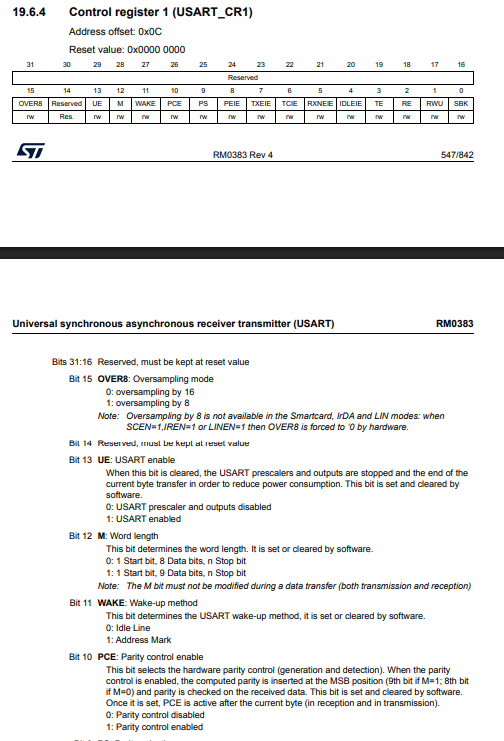
\includegraphics[width=0.8\linewidth]{imagens/USART_CR1_1.png}
    \caption{USART\_CR1\_1}
\end{figure}
\begin{figure}[H]
    \centering
    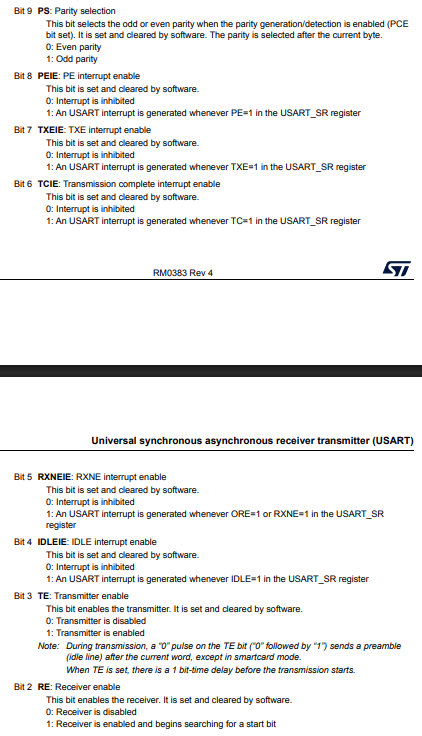
\includegraphics[width=0.8\linewidth]{imagens/USART_CR1_2.png}
    \caption{USART\_CR1\_2}
\end{figure}
\begin{figure}[H]
    \centering
    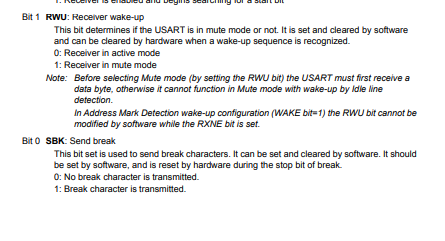
\includegraphics[width=0.8\linewidth]{imagens/USART_CR1_3.png}
    \caption{USART\_CR1\_3}
\end{figure}

\vspace{0.3cm}
\noindent\textbf{\texttt{USARTx->SR} (Status Register - O Painel de Luzes):}\\
É apenas de leitura. O hardware altera esses bits para te avisar das coisas.
\begin{itemize}
    \item \textbf{Bit 7 (TXE - Transmit Data Register Empty):} Se estiver em 1, significa que a caixa de saída está vazia e você pode colocar o próximo caractere.
    \item \textbf{Bit 5 (RXNE - Read Data Register Not Empty):} Se estiver em 1, a UART recebeu um byte do mundo externo e ele está pronto para você ler.
\end{itemize}

\begin{figure}[H]
    \centering
    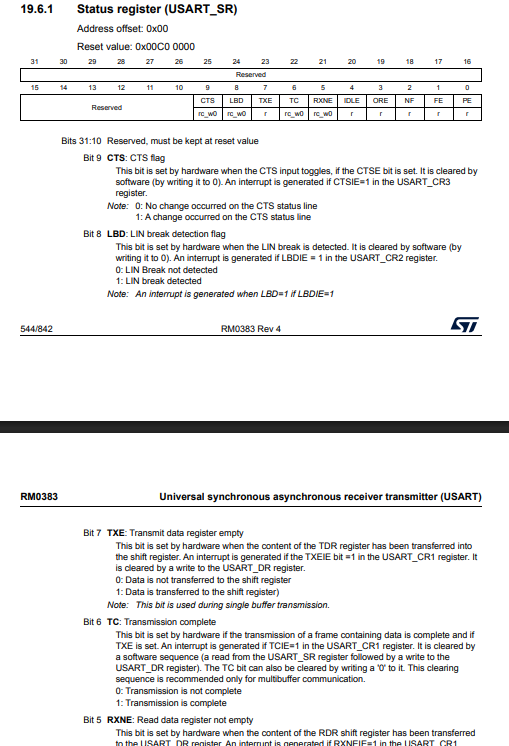
\includegraphics[width=0.8\linewidth]{imagens/USART_SR_1.png}
    \caption{USART\_SR\_1}
\end{figure}
\begin{figure}[H]
    \centering
    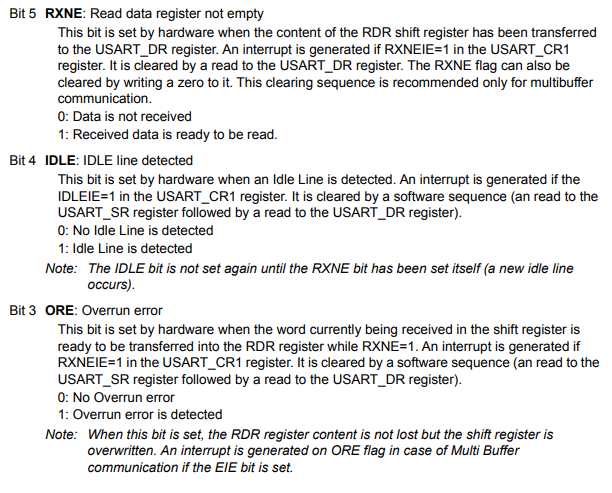
\includegraphics[width=0.8\linewidth]{imagens/USART_SR_2.png}
    \caption{USART\_SR\_2}
\end{figure}

\vspace{0.3cm}
\noindent\textbf{\texttt{USARTx->DR} (Data Register - A Caixa de Correio):}\\
É um registrador de 32 bits, mas só usamos os 8 bits mais baixos (porque enviamos 1 byte por vez).
\begin{itemize}
    \item Se você escrever nele (\texttt{USART2->DR = 'A';}), o hardware puxa o dado para um ``Shift Register'' interno (invisível para você) e começa a disparar os bits no pino TX. O bit TXE cai para 0 até ele terminar.
    \item Se você ler ele (\texttt{char c = USART2->DR;}), você pega o byte que chegou. Ler esse registrador zera a flag \texttt{RXNE} automaticamente.
\end{itemize}

\begin{figure}[H]
    \centering
    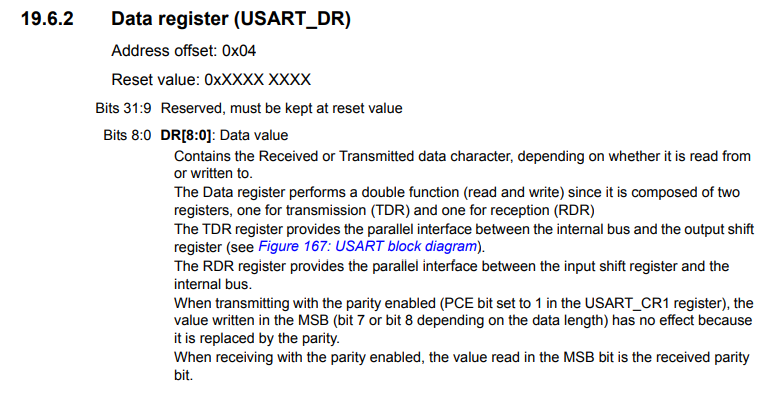
\includegraphics[width=0.8\linewidth]{imagens/USART_DR.png}
    \caption{USART\_DR}
\end{figure}

\vspace{0.3cm}
\noindent\textbf{\texttt{USARTx->BRR} (Baud Rate Register):}\\
Como explicado antes, dividido entre Mantissa (Bits 15 a 4) e Fração (Bits 3 a 0) para dividir o Clock e gerar a velocidade correta, levando o fator de \textit{Oversampling} em consideração.

\begin{figure}[H]
    \centering
    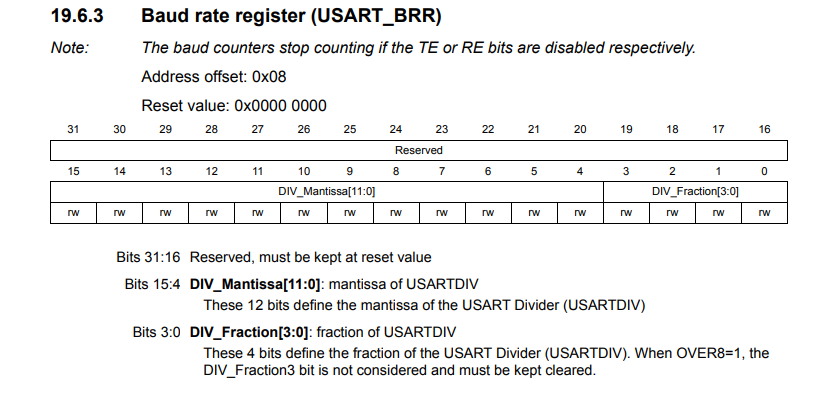
\includegraphics[width=0.8\linewidth]{imagens/USART_BRR.png}
    \caption{USART\_BRR}
\end{figure}

\textbf{A Matemática do Baud Rate no F4:}\\
Lembra que o Clock (APB) afeta os periféricos? Se a sua USART2 está no barramento APB1 rodando a 48 MHz, e você quer um Baud Rate de 115200, o hardware precisa saber como dividir esse clock de forma fracionada.
A fórmula do manual da ST é:
\[ USARTDIV = \frac{f_{PCLK}}{16 \times BaudRate} \]
No nosso exemplo:
\[ USARTDIV = \frac{48000000}{16 \times 115200} = 26.0416 \]
O STM32F4 divide o registrador BRR em duas partes: a Mantissa (a parte inteira, que vale 26) e a Fração (a parte decimal 0.0416 multiplicada por 16).
Fração: $16 \times 0.0416 = 0.66$ (arredondamos para 1).
O registrador pede a Mantissa deslocada 4 casas para a esquerda, somada à Fração.

\begin{lstlisting}[language=C]
/* Configuracao do Baud Rate (Exemplo Bare-Metal F4) */
USART2->BRR = (26UL << 4) | 1; 
\end{lstlisting}

\textbf{Como Enviar e Receber direto no Hardware:}
\begin{lstlisting}[language=C]
/* Enviar um caractere ('A') */
void UART_SendChar(char c)
{
  /* 1. Trava a CPU em um loop vazio ENQUANTO a caixa de saida estiver cheia (TXE == 0) */
  while (!(USART2->SR & (1UL << 7))); 
  
  /* 2. Joga o caractere na caixa de correio. O hardware assume o envio. */
  USART2->DR = c; 
}

/* Receber um caractere (Polling) */
char UART_ReceiveChar(void)
{
  /* 1. Trava a CPU ENQUANTO a flag de ``dado nao lido'' for zero (RXNE == 0) */
  while (!(USART2->SR & (1UL << 5))); 
  
  /* 2. Le a caixa de correio. O simples ato de ler ZERA a flag RXNE automaticamente! */
  return (char)(USART2->DR); 
}
\end{lstlisting}

\subsubsection{A Mágica do Printf (Redirecionamento Padrão)}
A função \texttt{printf()} pertence à biblioteca padrão do C (\texttt{<stdio.h>}). Em um computador normal, ela manda o texto para o terminal do sistema operacional (Windows/Linux). Mas em um microcontrolador Bare-Metal, não existe sistema operacional. Se você chamar \texttt{printf("Ola");} logo de cara, o código não vai fazer nada, porque a biblioteca não faz ideia de qual pino físico usar para ``falar''.

Para fazer a mágica acontecer, precisamos criar uma ponte entre a biblioteca do C e o nosso hardware (a UART). Fazemos isso sobrescrevendo (\textit{overriding}) a função de baixo nível que o \texttt{printf} aciona nos bastidores para cuspir os caracteres.
Dependendo do compilador que você usa, a função alvo muda:

\textbf{Para o GCC (STM32CubeIDE):}\\
O compilador GCC usa a função \texttt{\_write} para enviar dados para a saída padrão. Basta colocar este bloco de código no seu \texttt{main.c} (geralmente na seção \texttt{/* USER CODE BEGIN 4 */}):

\begin{lstlisting}[language=C]
/* ========================================================== */
/* REDIRECIONAMENTO DO PRINTF (GCC / STM32CubeIDE)            */
/* ========================================================== */
#include <stdio.h> /* Obrigatorio incluir la no topo do main.c */

/* Referencia externa para a UART que voce configurou (ex: USART2) */
extern UART_HandleTypeDef huart2;

/* Sobrescreve a funcao nativa _write */
int _write(int file, char *ptr, int len)
{
  /* Usa a HAL para enviar o array de caracteres gerado pelo printf */
  /* HAL_MAX_DELAY garante que a CPU espere o tempo que for necessario */
  HAL_UART_Transmit(&huart2, (uint8_t*)ptr, len, HAL_MAX_DELAY);
  
  return len;
}
\end{lstlisting}

\textbf{Para o compilador ARM (Keil MDK):}\\
A biblioteca padrão do Keil aciona a função \texttt{fputc} (caractere único):
\begin{lstlisting}[language=C]
#include <stdio.h>
extern UART_HandleTypeDef huart2;

int fputc(int ch, FILE *f)
{
  /* Envia um caractere por vez */
  HAL_UART_Transmit(&huart2, (uint8_t *)&ch, 1, HAL_MAX_DELAY);
  return ch;
}
\end{lstlisting}

\textbf{Como usar no código:}\\
Depois de colar essa função de redirecionamento correspondente à sua IDE, você nunca mais precisará montar arrays e chamar \texttt{HAL\_UART\_Transmit} manualmente para mandar mensagens de log. Em qualquer lugar do seu código, você pode simplesmente usar:
\begin{lstlisting}[language=C]
int temperatura = 25;
printf("Sistema iniciado com sucesso!\r\n");
printf("A temperatura atual e: %d graus.\r\n", temperatura);
\end{lstlisting}

\textbf{Aviso Importante sobre Ponto Flutuante (\%f):} Por padrão, compiladores para sistemas embarcados (como o STM32CubeIDE) desabilitam o suporte a números fracionários (floats) no \texttt{printf} para economizar memória Flash. Se você tentar rodar \texttt{printf("Valor: \%f", 3.14);}, o número não vai aparecer.
Para consertar isso no CubeIDE, você precisa ir nas propriedades do projeto: \textit{Project > Properties > C/C++ Build > Settings > MCU Settings} e marcar a caixa \textit{``Use float with printf from newlib-nano''}.

\subsubsection{O \texttt{HAL\_UART\_Receive\_IT} recebe só um caractere?}
No nosso exemplo, sim, ele recebe apenas um caractere porque passamos o tamanho 1 como último argumento. A função original permite que você peça 10, 20 ou 100 caracteres.
\textbf{Por que pedimos apenas 1 no mundo real?}
Na comunicação serial assíncrona, você quase nunca sabe quantos caracteres o PC ou o sensor vai te mandar. Se você configurar \texttt{HAL\_UART\_Receive\_IT(\&huart2, buffer, 10);}, a interrupção só vai ser acionada quando o 10º caractere chegar.
Se o usuário digitar ``Oi'', o seu microcontrolador vai ficar esperando eternamente pelas outras 8 letras e nunca vai processar a mensagem. Lendo de 1 em 1, você consegue analisar cada letra que chega (por exemplo, checar se a letra é um \texttt{\textbackslash n} ou \texttt{\textbackslash r}, que indicam que o usuário apertou ``Enter'' e a mensagem acabou).

\subsubsection{A Matemática: Por que dividir por 16? (Oversampling)}
Na fórmula do Baud Rate, o Clock é dividido por $16 \times BaudRate$. Esse 16 mágico vem de uma técnica de hardware chamada \textit{Oversampling} (Superamostragem).



Como a UART não tem um pino de Clock para sincronizar perfeitamente o momento de ler o bit, o receptor precisa adivinhar o centro exato do pulso elétrico para não ler ``lixo''.
Para fazer isso, o hardware da UART não lê o pino apenas 1 vez por bit. Ele lê o pino 16 vezes absurdamente rápido durante a duração de um único bit.
A UART pega as amostras do meio (as leituras 8, 9 e 10) e faz uma ``votação''. Se a maioria for 1, ele crava que o bit é 1. Isso filtra ruídos elétricos (\textit{spikes}) na linha.
Logo, para que o hardware consiga bater 16 vezes dentro de um único pulso de Baud Rate, a ``engrenagem'' do relógio da UART precisa girar 16 vezes mais rápido que a taxa de comunicação.

\subsubsection{UART vs USART, Handlers e o misterioso \texttt{huart2}}
\textbf{A Diferença da Sigla:}
\begin{itemize}
    \item \textbf{UART:} \textit{Universal Asynchronous Receiver-Transmitter}. Só usa os pinos TX e RX.
    \item \textbf{USART:} \textit{Universal Synchronous/Asynchronous Receiver-Transmitter}. O hardware possui um pino extra (o pino de Clock - CK). Ele pode funcionar de forma Síncrona (parecido com o SPI), mas na prática embarcada, 99\% das vezes configuramos a USART para agir no modo Assíncrono comum, ignorando o pino de clock.
\end{itemize}

\textbf{Os Handlers e o \texttt{huart2}:}\\
Um microcontrolador parrudo como o STM32F411 possui 3 periféricos USART independentes no silício (USART1, USART2 e USART6). Se você quiser, pode ligar a placa em um GPS, em um módulo Bluetooth e no PC ao mesmo tempo.
Cada um deles recebe um ``Handle'' (uma struct de controle da HAL): \texttt{huart1}, \texttt{huart2} e \texttt{huart6}.

\textbf{Por que todo mundo usa o \texttt{huart2} nos exemplos?} Nas placas de desenvolvimento da ST (linhas Nucleo) e em algumas Black Pills, os pinos PA2 e PA3 (que pertencem fisicamente à USART2) estão soldados de fábrica no chip ST-Link da placa. O ST-Link converte o sinal dessa USART2 diretamente para o cabo USB. É por isso que você espeta o cabo no PC e consegue ler os dados no terminal sem precisar de conversores externos!

% ==========================================
% I2C Functions (Inter-Integrated Circuit)
% ==========================================
\subsection{I2C Functions (Inter-Integrated Circuit)}

\begin{figure}[H]
    \centering
    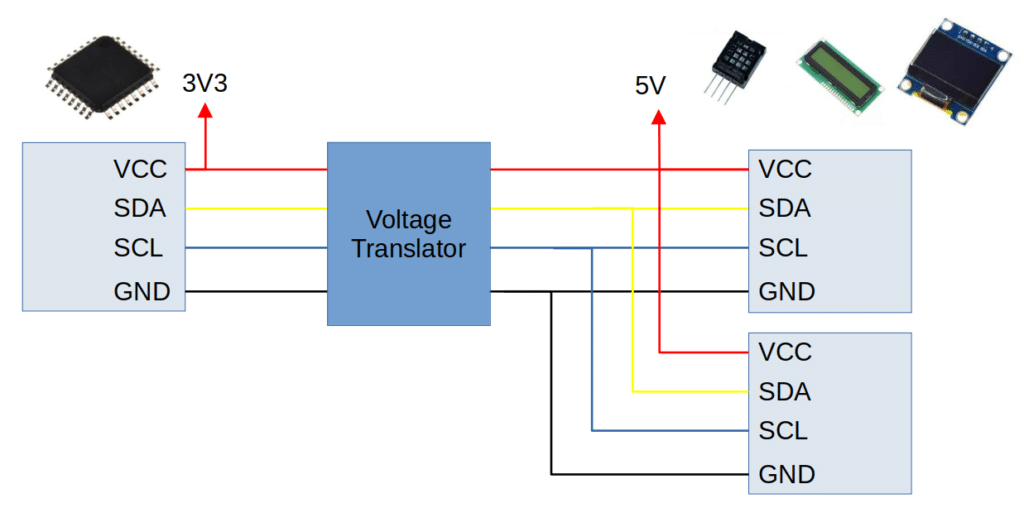
\includegraphics[width=0.8\linewidth]{imagens/I2C.png}
    \caption{I2C}
    \label{fig:i2c}
\end{figure}

O I2C (lê-se ``I ao quadrado C'' ou ``I-two-C'') foi criado pela Philips para resolver um problema grave: como conectar dezenas de chips em uma placa sem precisar de dezenas de fios de cobre cruzando o circuito.

A solução foi criar um Barramento (Bus) usando apenas dois fios:
\begin{itemize}
    \item \textbf{SCL (Serial Clock):} O pino que dita o ritmo da conversa (síncrono).
    \item \textbf{SDA (Serial Data):} O pino por onde os dados trafegam nos dois sentidos (\textit{Half-Duplex}).
\end{itemize}

\subsubsection{A Arquitetura Física e o Dreno Aberto (Open-Drain)}
Diferente da UART ou do SPI, onde um pino empurra ativamente 3.3V (ALTO) ou 0V (BAIXO), os pinos do I2C operam em modo \textbf{Open-Drain} (Dreno Aberto).

Isso significa que o microcontrolador e os sensores só conseguem puxar a linha para o GND (0V). Nenhum chip no barramento tem a capacidade de injetar 3.3V na linha. Se dois chips tentarem falar ao mesmo tempo, um empurrando 3.3V e outro 0V, ocorreria um curto-circuito. O Dreno Aberto previne isso. Ele só tem duas opções:
\begin{itemize}
    \item Puxar a linha para o Terra (0V) para enviar um bit 0.
    \item ``Soltar'' a linha (ficar em alta impedância) para enviar um bit 1.
\end{itemize}



Como a linha fica ``solta'' no bit 1, precisamos instalar resistores de Pull-Up externos (geralmente de 4.7k$\Omega$ ou 10k$\Omega$) ligados ao 3.3V. É a física do resistor que puxa a tensão para cima quando ninguém está puxando para baixo.

\textbf{No STM32CubeMX:}\\
Quando você ativa o I2C, o CubeMX automaticamente vai na configuração dos pinos do SDA e SCL e altera o \textit{GPIO Output Level} para \textit{Open Drain}. Você pode verificar isso clicando no pino na visão do chip.

\textbf{No Bare-Metal (Registrador OTYPER):}\\
Para fazer isso na unha, além de configurar o pino como Alternate Function (como fizemos no PWM e UART), você precisa ir ao registrador de Tipo de Saída (OTYPER) da porta GPIO e setar o bit correspondente para 1.
\begin{lstlisting}[language=C]
/* Exemplo: SDA no PB9 e SCL no PB8 */
GPIOB->MODER  |= (10UL << 16); // PB8 e PB9 como Alternate Function (10)
GPIOB->OTYPER |= (3UL << 8);   // Seta os bits 8 e 9 como 1 (Open-Drain)
GPIOB->PUPDR  |= (5UL << 16);  // Liga os Pull-Ups internos (01) por precaucao
\end{lstlisting}

\subsubsection{O Protocolo: Mestres, Escravos e Endereços}
No I2C, os dispositivos são divididos em hierarquia:
\begin{itemize}
    \item \textbf{Master (Mestre):} É o seu STM32. Só ele pode gerar o sinal de Clock (SCL) e decidir quem vai falar e quando.
    \item \textbf{Slave (Escravo):} São os sensores. Eles ficam calados até que o Mestre os chame pelo nome.
\end{itemize}

\textbf{O Endereçamento (7 bits):}\\
Como todos estão nos mesmos dois fios, o Mestre precisa ``gritar'' o endereço do Escravo que ele quer acessar. Todo dispositivo I2C tem um endereço fixo de fábrica (de 0 a 127). Por exemplo, o acelerômetro MPU6050 geralmente tem o endereço \texttt{0x68}.

A anatomia de uma conversa I2C é assim:
\begin{enumerate}
    \item \textbf{Start Condition:} O Mestre puxa o SDA para baixo enquanto o SCL está alto. Isso avisa: ``Atenção todos, a conversa vai começar''.
    \item \textbf{Endereço + R/W:} O Mestre envia os 7 bits do endereço do MPU6050, mais 1 bit no final dizendo se ele quer Ler (1) ou Escrever (0). Total: 8 bits.
    \item \textbf{ACK (Acknowledge):} O Mestre solta a linha. Se o MPU6050 estiver vivo e ouvir seu endereço, ele puxa a linha para baixo, enviando um bit de confirmação (ACK).
    \item \textbf{Dados:} Os bytes de dados começam a fluir pelo SDA no ritmo do SCL.
    \item \textbf{Stop Condition:} O Mestre solta a linha SDA enquanto SCL está alto, encerrando o pacote.
\end{enumerate}

\subsubsection{I2C com HAL (A Função de Ouro)}
A HAL esconde toda a complexidade de gerar os sinais de Start, ACK e Stop.
Para operações simples (mandar ou receber um pacote genérico de dados), usamos:
\begin{lstlisting}[language=C]
HAL_I2C_Master_Transmit(&hi2c1, endereco_escravo, dados, tamanho, timeout);
HAL_I2C_Master_Receive(&hi2c1, endereco_escravo, buffer, tamanho, timeout);
\end{lstlisting}

\textbf{Atenção ao Endereço na HAL:} O STM32 exige que o endereço do dispositivo já venha com o espaço do bit R/W alocado. Ou seja, você precisa pegar o endereço original do sensor e dar um \textit{Shift Left} de 1 bit (\texttt{endereco << 1}). Muitos esquecem isso e acham que o sensor está quebrado.

\vspace{0.3cm}
\noindent\textbf{A Função de Ouro: HAL\_I2C\_Mem\_Read / Write}\\
Na vida real, sensores I2C possuem dezenas de registradores internos (um para o eixo X, outro para a temperatura, etc). Para ler a temperatura, você não apenas recebe dados; você precisa primeiro escrever o endereço do registrador interno da temperatura, e depois ler o que o sensor responde.
A HAL tem uma função específica que faz essas duas etapas de uma vez só:
\begin{lstlisting}[language=C]
uint8_t temp_bruta[2];
uint8_t end_sensor = (0x68 << 1); // Endereco I2C do chip MPU6050 com shift
uint8_t reg_temp_out = 0x41;      // Endereco interno do registrador de temperatura no MPU6050

/* Le 1 byte do registrador 0x41 dentro do chip 0x68 */
HAL_I2C_Mem_Read(&hi2c1, end_sensor, reg_temp_out, I2C_MEMADD_SIZE_8BIT, &valor_temperatura, 2, 100);
\end{lstlisting}

\subsubsection{I2C no ``Bare Metal'' (O Desafio do Silício)}
Programar o I2C direto nos registradores do STM32 (especialmente na família F4 e mais antigas) é notoriamente complexo. Ao contrário da UART, onde olhamos apenas uma ou duas flags de status, o I2C da ST é uma \textbf{Máquina de Estados Finita} pesada.

Existem dois registradores de status (\texttt{I2C1->SR1} e \texttt{I2C1->SR2}) que mudam de valor sozinhos e geram uma sequência rigorosa de ``Eventos'' (EV5, EV6, EV8) que o programador deve limpar na ordem exata ditada pelo manual.

A sequência básica para enviar 1 byte via registradores é:
\begin{enumerate}
    \item \texttt{I2C1->CR1 |= (1<<8);} // Gera o START condition (Avisa o barramento).
    \item Espera o bit \texttt{SB} (Start Bit gerado) no SR1 virar 1.
    \item Joga o endereço do Escravo no registrador de dados (\texttt{I2C1->DR}).
    \item Espera a flag \texttt{ADDR} (Address matched) no SR1 virar 1.
    \item \textbf{A armadilha:} Para limpar a flag ADDR, você é obrigado a ler o SR1 e imediatamente ler o SR2. Se não fizer isso, o barramento trava.
    \item Espera a flag \texttt{TXE} (Transmit Empty) no SR1.
    \item Joga o byte de dado no \texttt{I2C1->DR}.
    \item \texttt{I2C1->CR1 |= (1<<9);} // Gera o STOP condition.
\end{enumerate}

\textbf{Resumo da Ópera para o I2C:} Salvo por razões estritas de otimização máxima ou aprendizado acadêmico, a imensa maioria dos sistemas embarcados da indústria utiliza a HAL ou LL para operar o I2C no STM32, pois as bibliotecas já implementam os tratamentos de todas as condições de erro (como \textit{Bus Error, Arbitration Lost e Acknowledge Failure}) que são um pesadelo de implementar manualmente.

O maior ``pega-ratão'' do I2C no silício da ST é a forma como você limpa as flags. Por exemplo, quando você envia o endereço do sensor, a flag \texttt{ADDR} sobe para 1. Para limpá-la e continuar a transmissão, você é fisicamente obrigado a ler o registrador \texttt{SR1} e depois ler o \texttt{SR2}. Se inverter a ordem ou não ler o \texttt{SR2}, o barramento trava para sempre.

Aqui está uma ``palhinha'' de como seria um código para iniciar a comunicação (Start Condition) e enviar o endereço do dispositivo:

\begin{lstlisting}[language=C]
/* Supondo barramento configurado a 100kHz nos registradores CR2, CCR e TRISE */

void I2C_IniciaEscrita(uint8_t endereco_sensor) 
{
    volatile uint32_t reg_temp;

    /* 1. Gera a condicao de START na linha (SDA desce enquanto SCL esta alto) */
    I2C1->CR1 |= (1UL << 8); // Seta o bit START

    /* 2. Aguarda o hardware confirmar que gerou o START com sucesso (Flag SB) */
    while (!(I2C1->SR1 & (1UL << 0))); 

    /* 3. Coloca o Endereco do Sensor no barramento + Bit de Escrita (0) */
    /* O ato de escrever no DR limpa a flag SB automaticamente */
    I2C1->DR = (endereco_sensor << 1) | 0x00; 

    /* 4. Aguarda o sensor reconhecer e responder com um ACK (Flag ADDR) */
    while (!(I2C1->SR1 & (1UL << 1))); 

    /* 5. A Magica de Limpeza da ST: 
          Para limpar a flag ADDR, devemos OBRIGATORIAMENTE ler SR1 e depois SR2 */
    reg_temp = I2C1->SR1;
    reg_temp = I2C1->SR2; 
    (void)reg_temp; // Evita warning de variavel nao usada no compilador

    /* O barramento agora esta livre para voce escrever os dados no I2C1->DR */
}
\end{lstlisting}

Depois de gerar o Start e o sensor responder ao endereço (ACK), o barramento fica travado esperando você agir. Temos duas vias a partir daqui:

\vspace{0.3cm}
\noindent\textbf{1. Escrevendo Dados (I2C\_EscreveByte)}\\
Para enviar os dados (seja um endereço de registrador interno ou uma configuração), usamos o registrador \texttt{DR} e monitoramos duas flags cruciais no \texttt{SR1}: a \texttt{TXE} (Data Register Empty) e a \texttt{BTF} (Byte Transfer Finished).
\begin{lstlisting}[language=C]
void I2C_EscreveByte(uint8_t dado) 
{
    /* 1. Espera a ``caixa de saida'' ficar vazia (Flag TXE == 1) */
    while (!(I2C1->SR1 & (1UL << 7))); 
    
    /* 2. Joga o dado no registrador. O hardware comeca a mandar os bits pelo pino SDA */
    I2C1->DR = dado;
    
    /* 3. Espera a transferencia fisica de todos os 8 bits + ACK terminar (Flag BTF == 1) */
    /* Se voce nao esperar o BTF e ja mandar um STOP, o ultimo byte e cortado no meio! */
    while (!(I2C1->SR1 & (1UL << 2))); 
}
\end{lstlisting}

\vspace{0.3cm}
\noindent\textbf{2. Encerrando a Comunicação (I2C\_Stop)}\\
No I2C, você é obrigado a liberar a linha SDA e SCL para que outros sensores possam falar. Isso é feito gerando a condição de STOP no registrador \texttt{CR1}.
\begin{lstlisting}[language=C]
void I2C_GeraStop(void) 
{
    /* Seta o bit STOP (Bit 9). O hardware solta as linhas automaticamente. */
    I2C1->CR1 |= (1UL << 9); 
}
\end{lstlisting}

\vspace{0.3cm}
\noindent\textbf{3. Lendo Dados (A Pegadinha do NACK)}\\
Receber dados no Bare-Metal é a parte mais traiçoeira do silício do STM32. Lembra que o Master tem que avisar o sensor quando quer que ele pare de mandar dados? Fazemos isso enviando um \textbf{NACK} (Not Acknowledge) após o último byte que queremos.
Se formos ler apenas 1 byte, precisamos desligar o nosso gerador de ACK (\texttt{CR1}) e já engatilhar o STOP antes mesmo de ler o dado do registrador \texttt{DR}.
\begin{lstlisting}[language=C]
uint8_t I2C_LeUmByte(void) 
{
    uint8_t dado_recebido;

    /* 1. Desliga o ACK automatico (NACK no proximo byte) */
    I2C1->CR1 &= ~(1UL << 10); // Limpa o bit ACK (Bit 10)
    
    /* 2. Ja avisa o hardware que, assim que esse byte terminar, e para dar STOP */
    I2C1->CR1 |= (1UL << 9);   // Seta o bit STOP (Bit 9)
    
    /* 3. Espera o byte chegar completo no ``cofre'' de leitura (Flag RXNE == 1) */
    while (!(I2C1->SR1 & (1UL << 6))); 
    
    /* 4. Le o dado final (Isso limpa a flag RXNE automaticamente) */
    dado_recebido = I2C1->DR;
    
    return dado_recebido;
}
\end{lstlisting}

\textbf{O Fluxo Completo na Prática:}\\
Juntando a função da mensagem anterior com essas novas, se você quisesse escrever o valor \texttt{0x00} no registrador \texttt{0x6B} do acelerômetro \texttt{0x68} em Bare-Metal puro, o código ficaria limpo e procedural no seu \texttt{main()}:
\begin{lstlisting}[language=C]
/* Equivalente exato ao HAL_I2C_Mem_Write() */
I2C_IniciaEscrita(0x68);    // Manda START + Endereco do sensor (com bit de Write)
I2C_EscreveByte(0x6B);      // Manda o endereco da gaveta interna do sensor
I2C_EscreveByte(0x00);      // Manda o valor que queremos salvar la dentro
I2C_GeraStop();             // Libera o barramento
\end{lstlisting}

Aqui estão os registradores utilizados:
\begin{figure}[H]
    \centering
    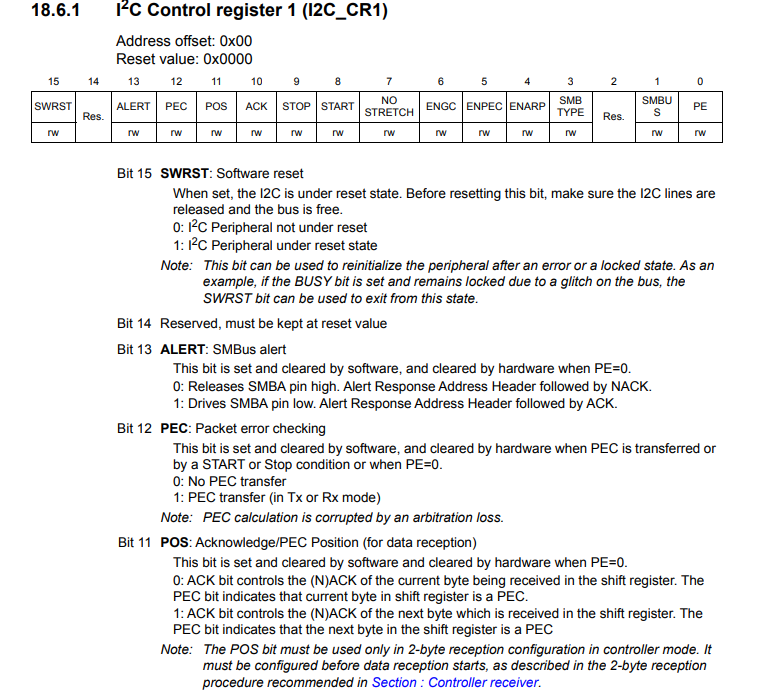
\includegraphics[width=0.8\linewidth]{imagens/I2C_CR1_1.png}
    \caption{I2C\_CR1\_1}
\end{figure}
\begin{figure}[H]
    \centering
    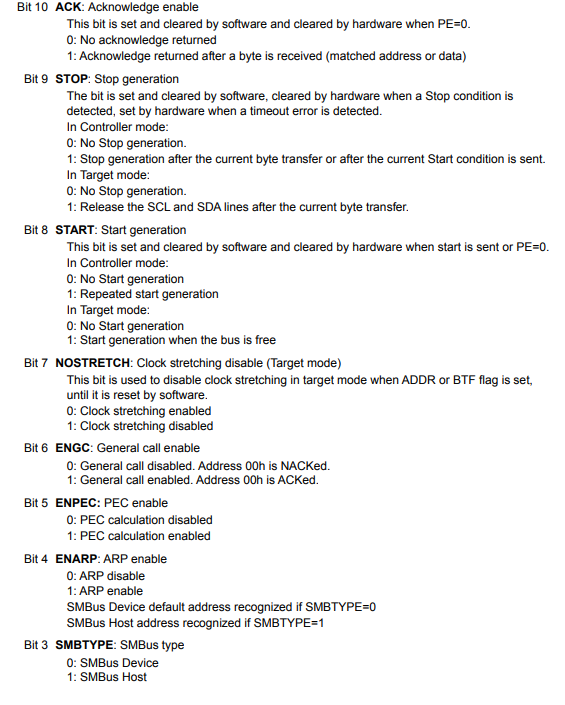
\includegraphics[width=0.8\linewidth]{imagens/I2C_CR1_2.png}
    \caption{I2C\_CR1\_2}
\end{figure}
\begin{figure}[H]
    \centering
    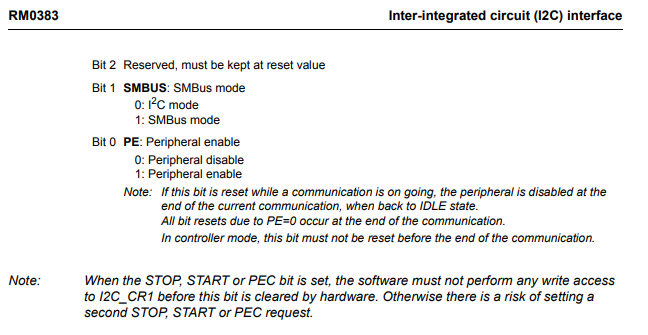
\includegraphics[width=0.8\linewidth]{imagens/I2C_CR1_3.png}
    \caption{I2C\_CR1\_3}
\end{figure}
\begin{figure}[H]
    \centering
    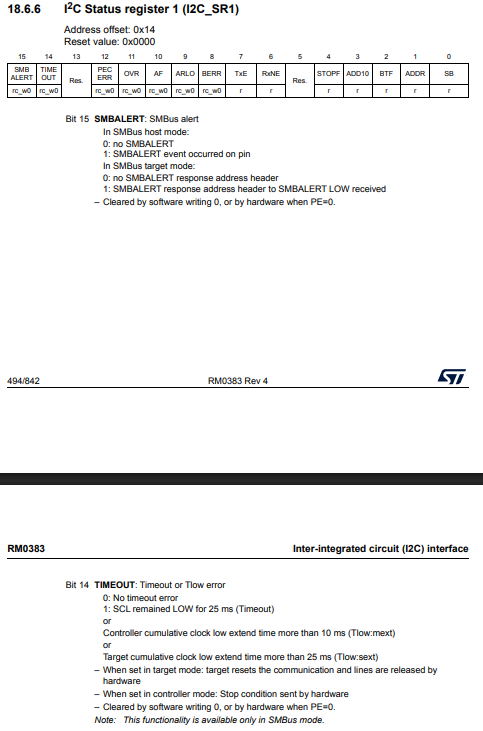
\includegraphics[width=0.8\linewidth]{imagens/I2C_SR1_1.png}
    \caption{I2C\_SR1\_1}
\end{figure}
\begin{figure}[H]
    \centering
    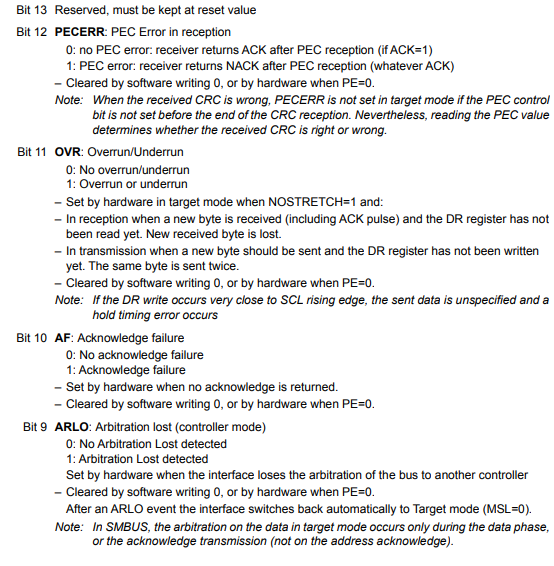
\includegraphics[width=0.8\linewidth]{imagens/I2C_SR1_2.png}
    \caption{I2C\_SR1\_2}
\end{figure}
\begin{figure}[H]
    \centering
    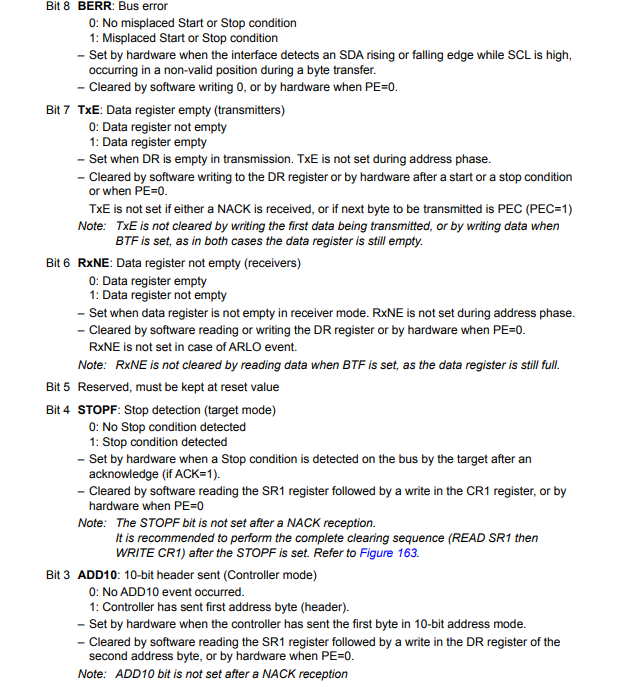
\includegraphics[width=0.8\linewidth]{imagens/I2C_SR1_3.png}
    \caption{I2C\_SR1\_3}
\end{figure}
\begin{figure}[H]
    \centering
    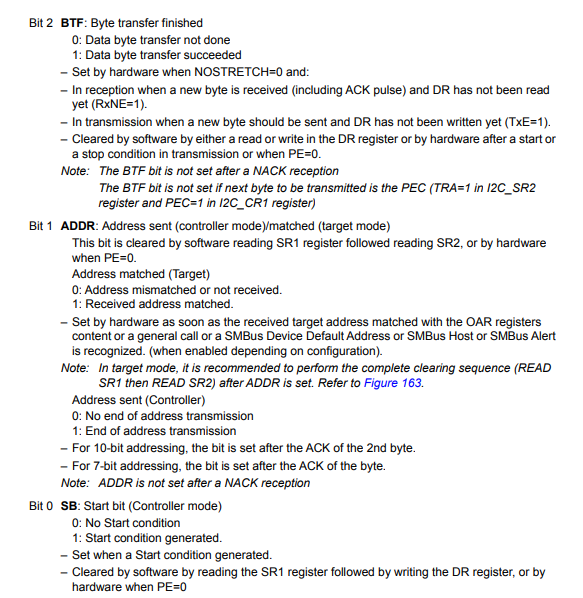
\includegraphics[width=0.8\linewidth]{imagens/I2C_SR1_4.png}
    \caption{I2C\_SR1\_4}
\end{figure}
\begin{figure}[H]
    \centering
    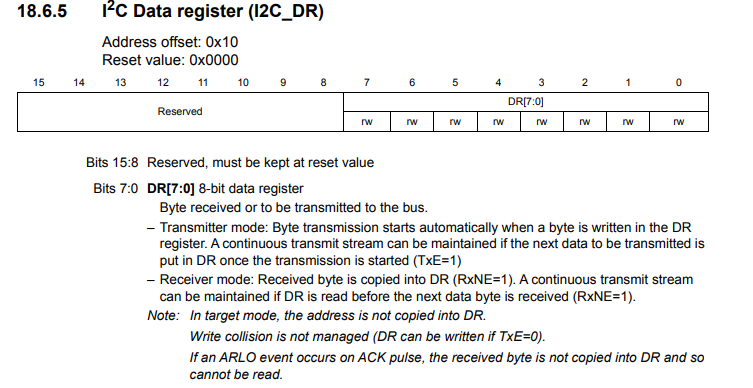
\includegraphics[width=0.8\linewidth]{imagens/I2C_DR.png}
    \caption{I2C\_DR}
\end{figure}

A complexidade desse sequenciamento de leitura de registradores de status é exatamente o motivo pelo qual engenheiros de sistemas embarcados adotam a biblioteca HAL para o I2C, mesmo quando escrevem o restante do código em Bare-Metal.

\subsubsection{A HAL: Master vs. Memória (As 4 Funções Principais)}
A HAL divide a comunicação I2C em duas grandes famílias: \textbf{Master} e \textbf{Mem} (Memory). A escolha entre elas depende inteiramente de com quem você está falando.

\textbf{A Diferença Fundamental:}
\begin{itemize}
    \item \textbf{Família Master (Transmit / Receive):} Envia ou recebe bytes ``crus'' diretamente para o endereço do dispositivo. O microcontrolador não especifica o que aquele byte significa. É usado para dispositivos simples, como um display LCD I2C ou um expansor de portas (PCF8574), que só precisam receber uma corrente contínua de dados.
    \item \textbf{Família Mem (Mem\_Write / Mem\_Read):} É a família feita especificamente para Sensores (Acelerômetros, Barômetros, etc.). Sensores são como mini-computadores que possuem dezenas de gavetas internas (registradores), cada uma com um endereço próprio (ex: \texttt{0x6B} para controle de energia, \texttt{0x3B} para leitura do Eixo X). As funções \texttt{Mem} enviam automaticamente o Endereço do Sensor seguido do Endereço do Registrador Interno antes de ler ou escrever o dado.
\end{itemize}

\vspace{0.3cm}
\noindent\textbf{1. A Família Master (Comunicação Direta)}\\
\textbf{Enviar Dados (\texttt{HAL\_I2C\_Master\_Transmit}):}\\
Você simplesmente aponta para o dispositivo e joga os bytes na linha.
\begin{lstlisting}[language=C]
uint8_t dados[2] = {0x01, 0xFF};
/* O endereco do dispositivo (ex: 0x27) OBRIGATORIAMENTE precisa ser deslocado 1 bit (<< 1) */
HAL_I2C_Master_Transmit(&hi2c1, (0x27 << 1), dados, 2, 100);
\end{lstlisting}

\textbf{Receber Dados (\texttt{HAL\_I2C\_Master\_Receive}):}\\
Você aponta para o dispositivo e fica escutando a linha para preencher o seu array. O dispositivo externo é quem dita o que está sendo enviado.
\begin{lstlisting}[language=C]
uint8_t buffer_recepcao[4];
/* O microcontrolador gera os pulsos de Clock, e o dispositivo envia 4 bytes */
HAL_I2C_Master_Receive(&hi2c1, (0x27 << 1), buffer_recepcao, 4, 100);
\end{lstlisting}

\vspace{0.3cm}
\noindent\textbf{2. A Família Memória (Comunicação com Registradores Internos)}\\
\textbf{Escrever em um Registrador (\texttt{HAL\_I2C\_Mem\_Write}):}\\
Essa função é fundamental no \texttt{setup()} do seu código para configurar o sensor.
Exemplo prático: Para ``acordar'' o acelerômetro MPU6050, você precisa escrever o valor \texttt{0x00} no registrador interno \texttt{0x6B} (Power Management).
\begin{lstlisting}[language=C]
uint8_t valor_configuracao = 0x00;

/* Parametros: 
   1. Handle do I2C (&hi2c1)
   2. Endereco do Sensor MPU6050 (0x68 << 1)
   3. Endereco do Registrador Interno (0x6B)
   4. Tamanho do Endereco Interno (1 Byte -> I2C_MEMADD_SIZE_8BIT)
   5. Ponteiro para a variavel com o dado a ser escrito (&valor_configuracao)
   6. Quantidade de bytes a escrever (1)
   7. Timeout em ms (100) */
HAL_I2C_Mem_Write(&hi2c1, (0x68 << 1), 0x6B, I2C_MEMADD_SIZE_8BIT, &valor_configuracao, 1, 100);
\end{lstlisting}
\textit{O que o hardware faz por baixo dos panos:} Ele envia o bit de Start, envia o endereço do sensor com bit de escrita, aguarda o ACK, envia o byte \texttt{0x6B}, aguarda o ACK, envia o byte \texttt{0x00}, aguarda o ACK e envia o bit de Stop. A função \texttt{Mem\_Write} abstrai toda essa burocracia.

\textbf{Ler de um Registrador (\texttt{HAL\_I2C\_Mem\_Read}):}\\
É a função que você colocará dentro do seu \texttt{while(1)} ou engatilhará por timer para extrair os dados físicos continuamente. Você diz ao sensor de qual ``gaveta'' quer extrair os dados.
Exemplo: Ler 2 bytes de temperatura do barômetro BMP180 a partir do registrador \texttt{0xF6}.
\begin{lstlisting}[language=C]
uint8_t temperatura_bruta[2];

/* A assinatura e identica ao Mem_Write, mas o destino do ponteiro 
   agora e um buffer vazio onde a HAL vai salvar os dados lidos */
HAL_I2C_Mem_Read(&hi2c1, (0x77 << 1), 0xF6, I2C_MEMADD_SIZE_8BIT, temperatura_bruta, 2, 100);
\end{lstlisting}
\textit{O que o hardware faz por baixo dos panos (Repeated Start):} No I2C, para ler um registrador, você não pode simplesmente pedir a leitura. Você tem que iniciar uma Escrita para mandar o número do registrador (\texttt{0xF6}), e sem soltar o barramento, enviar um sinal de \textit{Repeated Start} mudando o modo para Leitura, para então o sensor devolver os 2 bytes. O \texttt{Mem\_Read} faz exatamente essa manobra avançada de forma invisível.

% ==========================================
% SPI (Serial Peripheral Interface)
% ==========================================
\subsection{SPI (Serial Peripheral Interface)}

\begin{figure}[H]
    \centering
    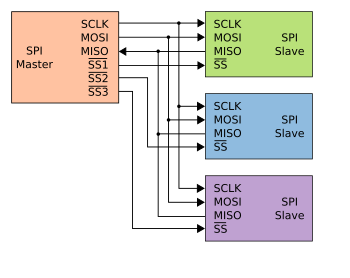
\includegraphics[width=0.8\linewidth]{imagens/SPI.png}
    \caption{SPI}
    \label{fig:spi}
\end{figure}

Criado pela Motorola, o SPI é um protocolo de barramento síncrono desenhado para velocidade extrema (facilmente ultrapassando a marca dos 10 a 50 Mbps).

Para alcançar essa velocidade, o SPI abandona a economia de fios do I2C e a comunicação Half-Duplex. Ele usa 4 fios dedicados e opera em modo \textbf{Full-Duplex} (fala e escuta ao exato mesmo tempo, como uma via de mão dupla).

\subsubsection{A Arquitetura Física (Os 4 Fios)}
Em um barramento SPI, sempre existe um Mestre (seu STM32) e um ou mais Escravos (sensores, memórias SD, displays). Os 4 pinos clássicos são:
\begin{itemize}
    \item \textbf{SCK (Serial Clock):} O relógio do sistema. Apenas o Mestre gera esse sinal para ditar o ritmo.
    \item \textbf{MOSI (Master Out, Slave In):} A via de transmissão. O Mestre fala, o Escravo escuta.
    \item \textbf{MISO (Master In, Slave Out):} A via de recepção. O Escravo fala, o Mestre escuta.
    \item \textbf{CS ou NSS (Chip Select / Slave Select):} O pino de ``Atenção''. Em vez de enviar um endereço pelo software (como no I2C), o Mestre usa um pino digital físico para selecionar com quem quer falar.
\end{itemize}

\subsubsection{O Conceito do Shift Register (A Troca Justa)}
A maior confusão de quem está aprendendo SPI é entender como enviar e receber funcionam. No SPI, enviar e receber são a mesma ação física.

Dentro do Mestre e do Escravo, existem registradores de deslocamento (\textit{Shift Registers}) conectados em formato circular pelos fios MOSI e MISO.



Toda vez que o Mestre gera 8 pulsos de Clock no fio SCK, ele ``empurra'' 8 bits para fora pelo MOSI. Ao mesmo tempo e no mesmo ritmo, esses mesmos 8 pulsos de Clock ``puxam'' 8 bits do Escravo para dentro do Mestre pelo MISO.

\textbf{Regra de Ouro do SPI:} Você \textbf{nunca} apenas ``lê'' ou apenas ``escreve''. Para cada byte que você envia, você recebe um byte (mesmo que seja lixo). Para receber um byte de um sensor, você é obrigado a enviar um byte (geralmente um byte vazio, \texttt{0x00} ou \texttt{0xFF}, chamado de \textit{Dummy Byte}) apenas para gerar o Clock necessário para o sensor responder.

\subsubsection{CPOL e CPHA (O Acordo do Relógio)}
Como não existe um padrão universal de fábrica, cada sensor inventa sua própria regra de como ler o relógio. O STM32 precisa se adaptar a eles configurando dois bits:
\begin{itemize}
    \item \textbf{CPOL (Clock Polarity):} Define se o relógio em repouso fica em 0V (Low) ou 3.3V (High).
    \item \textbf{CPHA (Clock Phase):} Define se os dados são lidos na primeira borda do relógio (subida) ou na segunda borda (descida).
\end{itemize}
Isso gera os \textbf{4 Modos do SPI} (Modo 0, 1, 2 e 3). Se o STM32 estiver no Modo 0, mas o datasheet do sensor exigir o Modo 3, a comunicação retornará apenas lixo.

\subsubsection{Chip Select (O Endereçamento Físico)}
Como não há endereços no protocolo, todos os escravos ficam conectados aos mesmos fios SCK, MOSI e MISO. O que impede a bagunça? O pino CS.

Cada escravo no barramento precisa ter um pino CS exclusivo ligado a um pino GPIO qualquer do seu STM32. O pino CS é Ativo em Baixo (\textit{Active Low}).
\begin{itemize}
    \item Enquanto o pino CS estiver em ALTO (3.3V), o escravo ignora o relógio, ignora o MOSI e deixa o seu próprio pino MISO em alta impedância (desconectado) para não atrapalhar os outros.
    \item Quando o Mestre puxa o CS de um escravo para BAIXO (0V), esse escravo ``acorda'' e passa a conversar no barramento.
\end{itemize}

\subsubsection{SPI com HAL (A Armadilha Comum)}
A biblioteca HAL tem as funções \texttt{HAL\_SPI\_Transmit} e \texttt{HAL\_SPI\_Receive}. Mas, devido à natureza Full-Duplex do hardware, a função mais segura e representativa da realidade é a \texttt{HAL\_SPI\_TransmitReceive}.

\textbf{A Armadilha (Hardware NSS vs Software):} No CubeMX, 99\% dos desenvolvedores desativam o controle de hardware do pino CS (NSS) e o configuram como um GPIO Output comum. A HAL \textbf{não gerencia} esse pino para você. É sua responsabilidade abaixar o pino antes da função, e levantá-lo depois.

\begin{lstlisting}[language=C]
/* Exemplo: Lendo o registrador WHO_AM_I (0x75) de um sensor SPI */

uint8_t dado_enviado[2];
uint8_t dado_recebido[2];

/* Byte 0: Endereco do registrador (O MSB em 1 geralmente indica Leitura no SPI) */
dado_enviado[0] = 0x75 | 0x80; 
/* Byte 1: Dummy byte (0x00) apenas para gerar clock para a resposta do sensor */
dado_enviado[1] = 0x00; 

/* 1. ACORDA O SENSOR: Puxa o CS para LOW (0V) */
HAL_GPIO_WritePin(GPIOA, GPIO_PIN_4, GPIO_PIN_RESET);

/* 2. REALIZA A TROCA (Envia 2 bytes, recebe 2 bytes simultaneamente) */
HAL_SPI_TransmitReceive(&hspi1, dado_enviado, dado_recebido, 2, 100);

/* 3. LIBERA O SENSOR: Puxa o CS de volta para HIGH (3.3V) */
HAL_GPIO_WritePin(GPIOA, GPIO_PIN_4, GPIO_PIN_SET);

/* O resultado final e util estara em dado_recebido[1] */
\end{lstlisting}

\subsubsection{SPI no ``Bare-Metal'' (A Volta da Simplicidade)}
Diferente do pesadelo de estados que é o I2C no nível dos registradores, o SPI no Bare-Metal é maravilhosamente simples.
A configuração inicial mexe no Registrador de Controle 1 (CR1) para definir o STM32 como Mestre, definir o Baud Rate, o CPOL/CPHA e ligar o periférico:

\begin{lstlisting}[language=C]
SPI1->CR1 |= (1UL << 2);  // MSTR: STM32 como Master
SPI1->CR1 |= (3UL << 3);  // BR: Divide o clock por 16
SPI1->CR1 |= (1UL << 9) | (1UL << 8); // SSM e SSI: Gestao de CS por software interno
SPI1->CR1 |= (1UL << 6);  // SPE: Liga o SPI
\end{lstlisting}

Para a comunicação, temos o Registrador de Dados (\texttt{SPI1->DR}) e o de Status (\texttt{SPI1->SR}). As flags são as mesmas da UART: \texttt{TXE} (Posso enviar mais?) e \texttt{RXNE} (Chegou algo?).

\begin{lstlisting}[language=C]
/* ========================================================== */
/* FUNCAO BASICA DE TROCA SPI NO BARE-METAL                   */
/* ========================================================== */
uint8_t SPI_TransferByte(uint8_t byte_out)
{
  /* 1. Espera o buffer de saida ficar livre (TXE == 1) */
  while (!(SPI1->SR & (1UL << 1)));
  
  /* 2. Coloca o dado no Data Register (Isso dispara o Clock fisico!) */
  SPI1->DR = byte_out;
  
  /* 3. Espera a recepcao terminar (RXNE == 1). Sempre recebemos de volta! */
  while (!(SPI1->SR & (1UL << 0)));
  
  /* 4. Le o dado que entrou pelo MISO */
  return (uint8_t)(SPI1->DR);
}

/* Como usar no codigo principal: */
// GPIOA->ODR &= ~(1UL << 4);               // Abaixa CS
// SPI_TransferByte(0x75 | 0x80);           // Envia endereco
// uint8_t valor = SPI_TransferByte(0x00);  // Envia Dummy, recebe Valor Real
// GPIOA->ODR |= (1UL << 4);                // Levanta CS
\end{lstlisting}

\textit{Dica de Engenharia:} No SPI, a ``escovação de bits'' é tão limpa e rápida que muitos desenvolvedores mesclam as abordagens: usam o CubeMX/HAL para configurar os Clocks e os Pinos sem dor de cabeça (o setup), mas escrevem as rotinas de TransmitReceive diretamente atacando o registrador \texttt{SPI->DR} para obter o máximo de velocidade e não travar a CPU ao ler sensores pesados.

Os registradores são esses:
\begin{figure}[H]
    \centering
    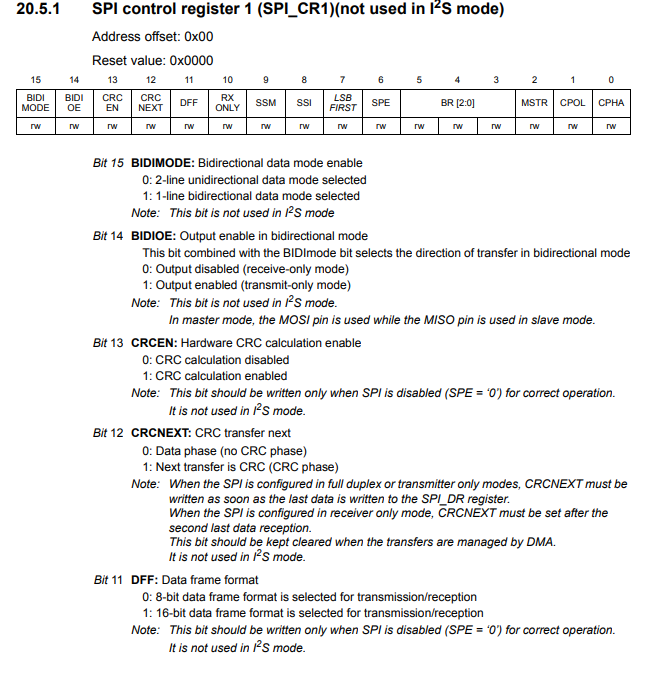
\includegraphics[width=0.8\linewidth]{imagens/SPI_CR1_1.png}
    \caption{SPI\_CR1\_1}
\end{figure}
\begin{figure}[H]
    \centering
    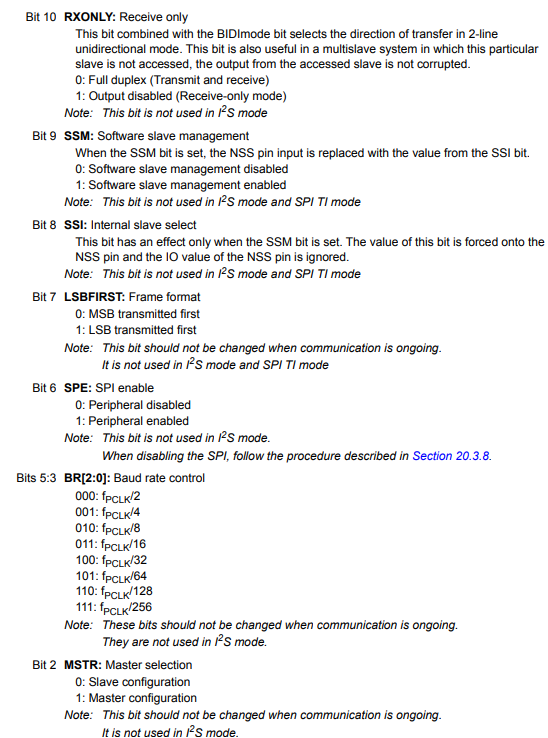
\includegraphics[width=0.8\linewidth]{imagens/SPI_CR1_2.png}
    \caption{SPI\_CR1\_2}
\end{figure}
\begin{figure}[H]
    \centering
    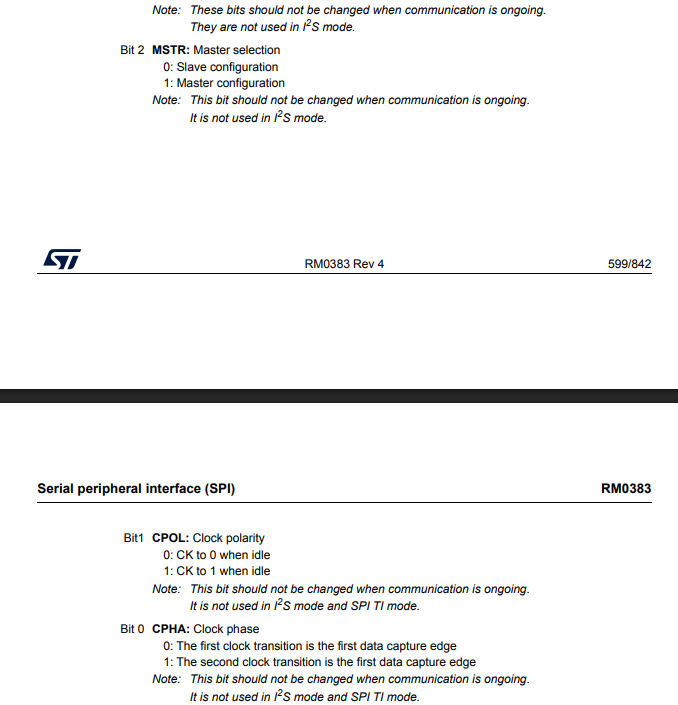
\includegraphics[width=0.8\linewidth]{imagens/SPI_CR1_3.png}
    \caption{SPI\_CR1\_3}
\end{figure}
\begin{figure}[H]
    \centering
    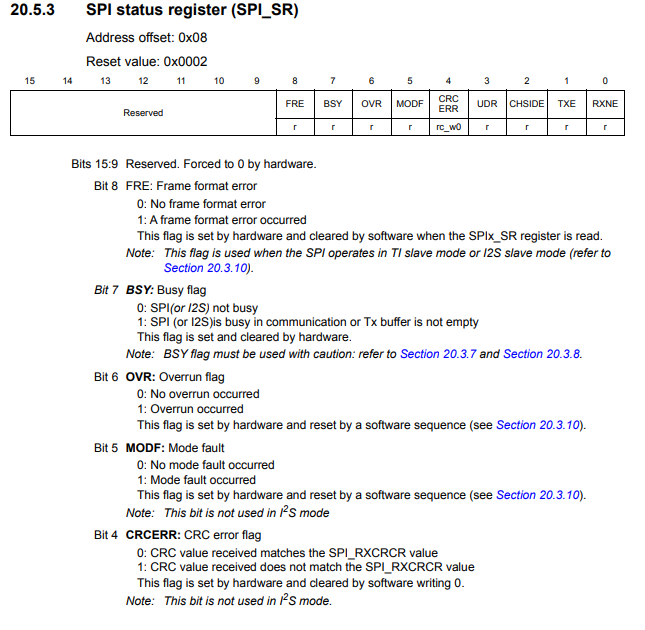
\includegraphics[width=0.8\linewidth]{imagens/SPI_SR_1.png}
    \caption{SPI\_SR\_1}
\end{figure}
\begin{figure}[H]
    \centering
    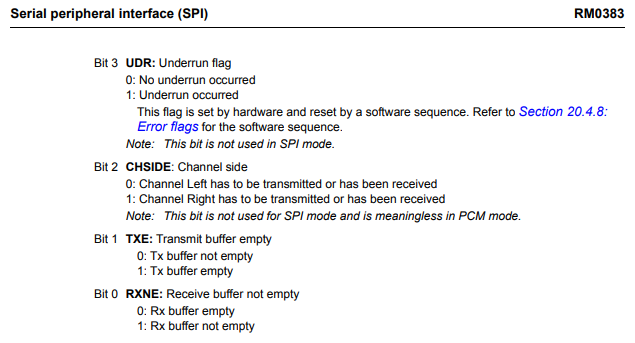
\includegraphics[width=0.8\linewidth]{imagens/SPI_SR_2.png}
    \caption{SPI\_SR\_2}
\end{figure}
\begin{figure}[H]
    \centering
    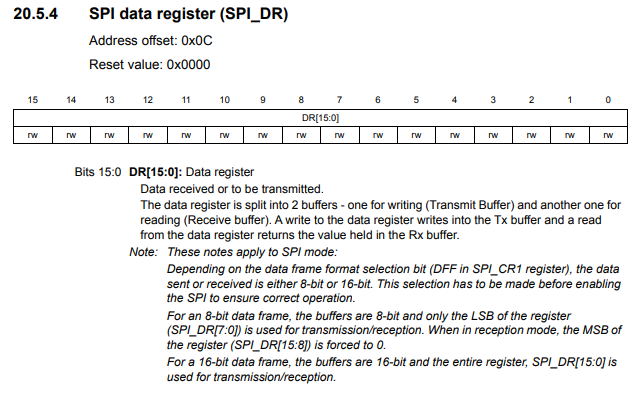
\includegraphics[width=0.8\linewidth]{imagens/SPI_DR.png}
    \caption{SPI\_DR}
\end{figure}

\vspace{0.3cm}
\noindent\textbf{O que significa 0x75 | 0x80? (O Bit de Leitura/Escrita)}\\
Lembra que no I2C, o microcontrolador avisa se quer Ler ou Escrever usando o último bit do endereço do dispositivo?
No SPI, como não existe endereço do dispositivo (nós usamos o pino CS para isso), como o sensor sabe se você quer apenas Ler o valor do registrador 0x75 ou se você quer Escrever um novo valor lá dentro?

A convenção adotada por 99\% dos fabricantes de sensores SPI (como os acelerômetros da InvenSense ou Bosch) é usar o MSB (\textit{Most Significant Bit} - O bit mais à esquerda) do \textbf{próprio endereço do registrador} para avisar a intenção.
A regra padrão nos datasheets é:
\begin{itemize}
    \item \textbf{MSB = 1:} É um comando de LEITURA.
    \item \textbf{MSB = 0:} É um comando de ESCRITA.
\end{itemize}

\textbf{A Matemática Bit a Bit:}\\
O registrador \texttt{WHO\_AM\_I} tem o endereço \texttt{0x75}. Em binário, isso é \texttt{0111 0101}.
Veja que o bit mais à esquerda (MSB) é 0. Se você enviar isso puro, o sensor vai achar que você quer escrever no registrador \texttt{0x75}.
Para forçar esse MSB a virar 1 sem alterar o resto do endereço, nós fazemos uma operação lógica OR (\texttt{|}) com o valor \texttt{0x80}.
O valor \texttt{0x80} em binário é exatamente \texttt{1000 0000}.
A conta que a CPU faz é:
\begin{verbatim}
  0111 0101  (0x75 - Endereco)
| 1000 0000  (0x80 - A Mascara de Leitura)
------------------
  1111 0101  (0xF5 - O byte final que vai para o fio MOSI)
\end{verbatim}

Ao receber \texttt{1111 0101}, o hardware do sensor entende: ``Opa, o primeiro bit é 1! Ele quer LER o que está no meu registrador \texttt{0111 0101}''.

\textbf{E para escrever?}\\
Se você quisesse configurar o sensor (escrever nele), bastaria enviar o \texttt{0x75} puro, ou, para ser extremamente rigoroso e seguro no código, usar uma máscara AND (\texttt{\&}) com \texttt{0x7F} (\texttt{0111 1111}) para garantir que o MSB seja forçado a zero:
\begin{lstlisting}[language=C]
dado_enviado[0] = 0x75 & 0x7F;
\end{lstlisting}

\vspace{0.3cm}
\noindent\textbf{Ler vs. Escrever no SPI (A Prática)}\\
Como o SPI troca bytes simultaneamente, a diferença entre ler e escrever está na intenção do que você coloca no fio MOSI no segundo byte da transação.

\textbf{O Fluxo de Leitura:}
Você quer saber o que está dentro de uma ``gaveta'' do sensor.
\begin{enumerate}
    \item Você envia o endereço da gaveta com o MSB em 1 (Comando de Leitura). O sensor responde com lixo.
    \item Você envia um Dummy Byte (\texttt{0x00}). Isso serve apenas para a sua placa gerar o Clock. O sensor aproveita esse Clock para empurrar o valor real da gaveta para você pelo MISO.
\end{enumerate}

\textbf{O Fluxo de Escrita:}
Você quer colocar um valor novo dentro da ``gaveta'' (ex: configurar a sensibilidade do giroscópio).
\begin{enumerate}
    \item Você envia o endereço da gaveta com o MSB em 0 (Comando de Escrita). O sensor responde com lixo.
    \item Em vez de um Dummy Byte, você envia o Dado Real que quer gravar (ex: \texttt{0x1A}). O sensor recebe esse dado e guarda na gaveta. Durante esse envio, o sensor te devolve lixo pelo MISO, mas você simplesmente ignora.
\end{enumerate}

\begin{lstlisting}[language=C]
/* Exemplo Pratico de ESCRITA: Configurando o registrador 0x1C com o valor 0x08 */
uint8_t tx_buffer[2];
tx_buffer[0] = 0x1C & 0x7F; // Forca MSB a 0 (Escrita)
tx_buffer[1] = 0x08;        // O dado real que queremos gravar

HAL_GPIO_WritePin(GPIOA, GPIO_PIN_4, GPIO_PIN_RESET); // Abaixa CS
HAL_SPI_Transmit(&hspi1, tx_buffer, 2, 100);          // Envia os 2 bytes
HAL_GPIO_WritePin(GPIOA, GPIO_PIN_4, GPIO_PIN_SET);   // Levanta CS
\end{lstlisting}

\subsubsection{Desmistificando as 3 Funções da HAL no SPI}
O hardware do SPI é sempre Full-Duplex (transmite e recebe ao mesmo tempo). No entanto, a ST criou três funções separadas na HAL para facilitar a vida do programador quando ele quer ignorar um dos lados da via.

\textbf{A) HAL\_SPI\_TransmitReceive (A função real)}\\
É a que mais reflete o hardware. Ela exige um buffer de envio e um buffer de recepção.
\textbf{Uso:} Leitura de sensores. Você manda o endereço e o dummy byte no \texttt{pTxData}, e captura a resposta no \texttt{pRxData}. Nada é descartado.

\textbf{B) HAL\_SPI\_Transmit (A função de envio cego)}\\
Você fornece apenas o buffer de envio (\texttt{pData}).
\textbf{O que a HAL faz por baixo dos panos:} Ela joga os seus bytes no fio MOSI. Como o hardware obriga o MISO a receber algo de volta, os bytes entram no registrador \texttt{SPI->DR}, mas a HAL ignora e descarta tudo o que chega.
\textbf{Uso:} Escrita de configurações em sensores (onde a resposta não importa) ou envio de pixels para telas (OLED/TFT), onde o fluxo de dados é 100\% unilateral.

\textbf{C) HAL\_SPI\_Receive (A função de recepção forçada)}\\
Você fornece apenas o buffer de recepção (\texttt{pData}).
\textbf{O que a HAL faz por baixo dos panos:} Para receber, o STM32 precisa gerar o Clock. Para gerar o Clock, ele precisa transmitir algo. A HAL automaticamente cria Dummy Bytes ocultos e os envia pelo MOSI repetidamente até preencher o seu buffer de recepção com os dados que estão chegando no MISO.
\textbf{Uso:} Raro em sensores de acelerômetro/giroscópio (pois eles exigem que você mande o endereço do registrador antes, o que obriga o uso do \texttt{TransmitReceive}). É mais usado na leitura bruta de cartões SD ou conversores ADC externos contínuos.

% ==========================================
% Observações sobre os Protocolos
% ==========================================
\subsection{Observações sobre os Protocolos}

\subsubsection{A Quantidade de Periféricos (Os Handlers hspiX, hi2cX, huartX)}
O microcontrolador (especificamente a arquitetura do STM32F411) não possui apenas ``um'' SPI ou ``um'' I2C. O silício contém múltiplos blocos de hardware independentes para o mesmo protocolo.
Cada um desses blocos físicos recebe um número, e na biblioteca HAL, isso se traduz no nome do Handle (a struct de controle).

\textbf{Quantos existem no chip?}
\begin{itemize}
    \item \textbf{USART:} 3 blocos físicos (\texttt{huart1}, \texttt{huart2} e \texttt{huart6}). \textit{Nota:} A numeração pula o 3, 4 e 5 porque a ST usa projetos base compartilhados com chips maiores (como o F407), cortando partes do silício nas versões mais baratas.
    \item \textbf{SPI:} 5 blocos físicos (\texttt{hspi1}, \texttt{hspi2}, \texttt{hspi3}, \texttt{hspi4}, \texttt{hspi5}).
    \item \textbf{I2C:} 3 blocos físicos (\texttt{hi2c1}, \texttt{hi2c2}, \texttt{hi2c3}).
\end{itemize}

\textbf{Faz diferença qual eu escolho usar?}\\
Sim, faz total diferença por três motivos de hardware:
\begin{enumerate}
    \item \textbf{A Velocidade do Barramento (APB1 vs APB2):} Lembra que o chip é dividido em uma via lenta (APB1, máx 50 MHz) e uma via rápida (APB2, máx 100 MHz)? O SPI1, SPI4 e SPI5 estão pendurados no APB2. Eles são feitos para velocidade extrema (ex: enviar dados para um display colorido). O SPI2 e SPI3 estão no APB1. Eles são limitados a metade da velocidade máxima. O mesmo vale para a UART: A USART1 e USART6 (APB2) são mais rápidas que a USART2 (APB1). Os barramentos I2C ficam todos no APB1.
    \item \textbf{O Roteamento Físico (Pinos):} Você não pode colocar o SPI1 em qualquer pino do chip. O multiplexador de funções alternativas (AFR) amarra periféricos específicos a pinos específicos. Se você já gastou os pinos do SPI1 para ligar um rádio, será obrigado a usar o SPI2 para ligar o cartão SD.
    \item \textbf{Conflito de DMA:} Se você for usar DMA para automatizar as transferências, cada periférico está mapeado fisicamente para um ``Stream'' específico do controlador DMA. Escolher mal pode gerar um gargalo onde dois periféricos tentam usar o mesmo canal de DMA ao mesmo tempo.
\end{enumerate}

\subsubsection{O Portão de Energia: Habilitando o Clock do Periférico}
Este é o erro número um de quem programa em Bare-Metal.

Um periférico no STM32 nasce morto. O hardware interno da UART, do I2C e do SPI não recebe o sinal de Clock por padrão. Isso é feito de propósito para economizar bateria: por que gastar energia girando as engrenagens internas do SPI4 se você não soldou nada nele?

Se você tentar escrever um dado no registrador de controle de um periférico cujo clock está desligado (ex: \texttt{SPI1->CR1 = 0x03;}), o processador ARM tenta acessar uma área de memória que está fisicamente ``sem energia''. O resultado é um \textit{Hard Fault} imediato: a CPU trava em uma interrupção de falha de hardware e o seu sistema congela.

\textbf{Como o Clock é ativado?}

\textbf{Na HAL:}\\
Você não vê isso no \texttt{main.c} porque o CubeMX esconde o acionamento do disjuntor de energia dentro das funções de inicialização de baixo nível (no arquivo \texttt{stm32f4xx\_hal\_msp.c}). Antes de configurar os pinos, a HAL chama macros específicas do RCC:
\begin{lstlisting}[language=C]
__HAL_RCC_SPI1_CLK_ENABLE();   // Liga a energia do SPI1
__HAL_RCC_USART2_CLK_ENABLE(); // Liga a energia da USART2
\end{lstlisting}

\textbf{No Bare-Metal:}\\
Você é o engenheiro eletricista do chip. Antes de tocar em qualquer registrador do SPI, I2C ou UART, você precisa olhar o datasheet, descobrir em qual barramento ele está, e ligar o bit correspondente no registrador de habilitação do RCC (\texttt{APB1ENR} ou \texttt{APB2ENR}).
\begin{lstlisting}[language=C]
/* Exemplo de inicializacao Bare-Metal correta do SPI1 */

/* 1. LIGA A ENERGIA: Habilita o Clock do SPI1 no barramento APB2 (Bit 12) */
RCC->APB2ENR |= (1UL << 12); 

/* 2. So agora e seguro tocar nos registradores do SPI1 */
SPI1->CR1 |= (1UL << 2); // Configura como Master
/* ... resto da configuracao ... */
\end{lstlisting}  

% ==========================================
% ARQUITETURA DE SOFTWARE E DRIVERS
% ==========================================
\section{Arquitetura de Software e Drivers}

\begin{figure}[H]
    \centering
    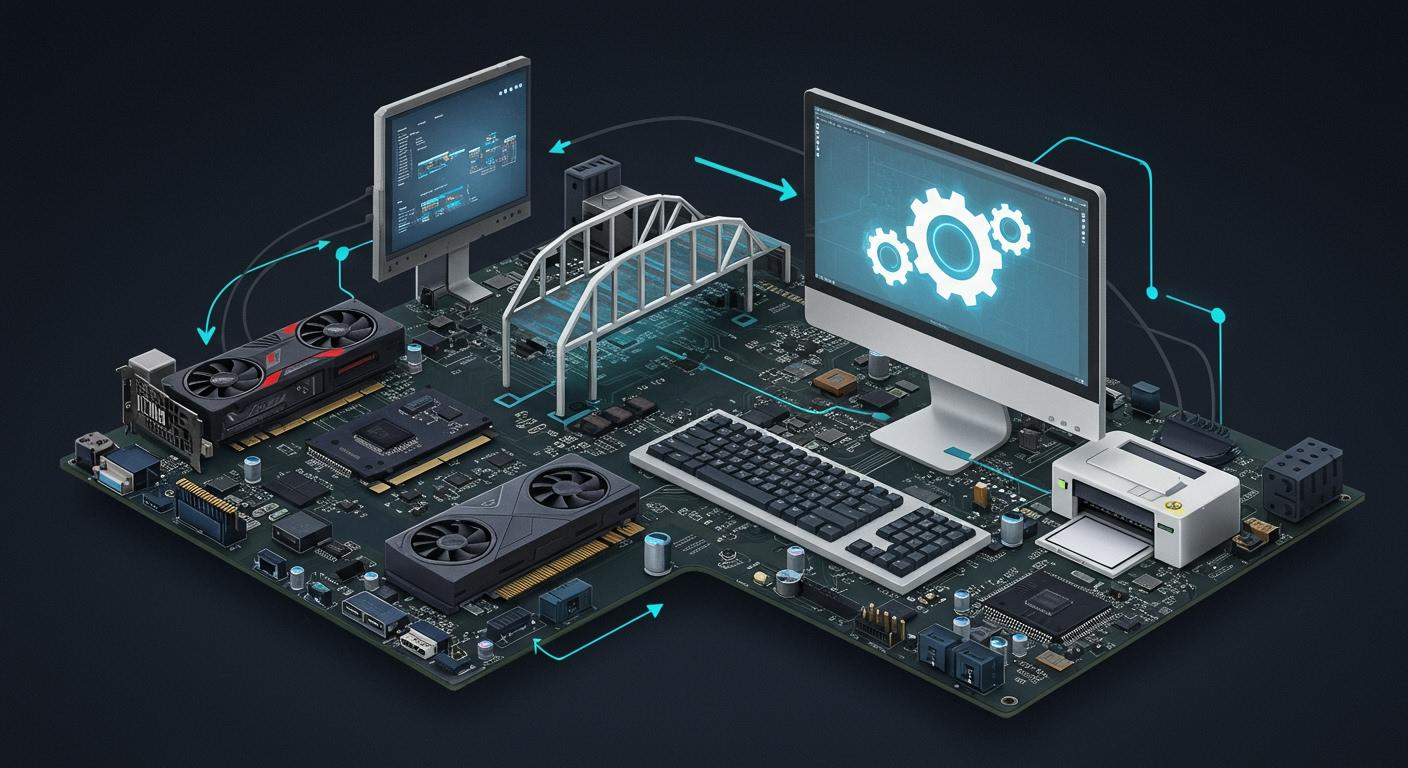
\includegraphics[width=0.8\linewidth]{imagens/Drivers.jpg}
    \caption{Drivers}
    \label{fig:drivers}
\end{figure}

Chegamos ao ponto de inflexão onde o código deixa de ser um experimento de bancada e vira um software de engenharia.

Quando você programa a lógica de um foguete ou de um sistema complexo, colocar chamadas de \texttt{HAL\_I2C\_Mem\_Read} e manipulação de registradores \texttt{SPI->DR} direto dentro do \texttt{while(1)} do \texttt{main.c} cria o temido ``Código Espaguete''. Fica impossível achar um erro ou reaproveitar o código em outro projeto.

A solução para isso é a \textbf{Modularização através de Drivers}.

No contexto de sistemas embarcados (C/C++), um ``Driver'' não é um arquivo executável que você instala no Windows. É simplesmente uma camada de abstração: um conjunto de arquivos (\texttt{.h} e \texttt{.c}) que esconde a complexidade do hardware e entrega funções fáceis de usar para o programa principal.

\subsection{Bibliotecas Inclusas (Os Drivers da ST)}
Quando você gera um projeto no CubeIDE, a ST já injeta uma série de drivers básicos no seu projeto. Eles servem exclusivamente para controlar o silício interno do microcontrolador:
\begin{itemize}
    \item \textbf{CMSIS (Cortex Microcontroller Software Interface Standard):} É o driver de mais baixo nível, feito pela própria ARM. Ele contém os endereços brutos da memória e os ponteiros mágicos (como o \texttt{\#define GPIOA} ou o \texttt{TIM2->CR1}). É a fundação do Bare-Metal.
    \item \textbf{HAL (Hardware Abstraction Layer):} É o driver de alto nível da ST. Ele entrega funções prontas como \texttt{HAL\_UART\_Transmit()} para que você não precise escovar os bits do CMSIS.
\end{itemize}

\textbf{O Problema:} A HAL sabe como acionar o barramento I2C do STM32, mas ela não faz a menor ideia do que é um sensor BMP180 ou um MPU6050. Ela não sabe quais são os endereços das ``gavetas'' internas desses sensores. Quem tem que ensinar isso ao sistema é você.

\subsection{Novo Driver do Usuário (A Sua Biblioteca)}
Para ler um barômetro ou atuar um servo motor mecânico, você deve criar o seu próprio Driver. A arquitetura correta em C exige a criação de dois arquivos na sua pasta de projeto (dentro de \texttt{Core/Inc} e \texttt{Core/Src}):

\vspace{0.3cm}
\noindent\textbf{1. O Arquivo Header (.h) - O Contrato (A Interface Pública)}\\
É aqui que você define as configurações do sensor (os endereços em hexadecimal), as estruturas de dados (\texttt{structs}) e os ``esqueletos'' das funções. O arquivo \texttt{.h} é o manual de instruções do seu driver. Quem for usar o seu sensor, só precisa ler este arquivo.
\textit{Regra de Ouro do Header (Include Guards):} Todo arquivo \texttt{.h} deve ser protegido contra múltiplas inclusões pelo compilador usando as diretivas \texttt{\#ifndef}, \texttt{\#define} e \texttt{\#endif}. Se você esquecer isso, o compilador tentará declarar as mesmas variáveis várias vezes e o código não vai compilar.

\vspace{0.3cm}
\noindent\textbf{2. O Arquivo Source (.c) - A Engenharia (A Implementação Privada)}\\
É aqui que a ``sujeira'' fica escondida. Neste arquivo, você inclui a biblioteca HAL, o CMSIS, e escreve a lógica bruta de I2C, SPI ou manipulação de registradores para fazer o sensor funcionar. O \texttt{main.c} nunca deve ver o que acontece aqui dentro.

\subsection{Exemplo Prático: Criando um Driver de Sensor (BMP180 via I2C)}
Vamos imaginar que estamos criando um driver para ler a temperatura de um barômetro I2C (endereço \texttt{0x77}).

\textbf{Passo 1: Criando o \texttt{bmp180.h} (Na pasta \texttt{Core/Inc})}
\begin{lstlisting}[language=C]
/* ================================================================= */
/* bmp180.h - Interface Publica do Driver                            */
/* ================================================================= */

/* INCLUDE GUARDS (Protecao obrigatoria em C) */
#ifndef BMP180_H_
#define BMP180_H_

#include <stdint.h> /* Para usar uint8_t, uint16_t */

/* 1. Definicoes de Hardware do Sensor (Tiradas do Datasheet) */
#define BMP180_I2C_ADDR      (0x77 << 1) /* Endereco I2C do chip */
#define BMP180_REG_TEMP_OUT  0xF6        /* Registrador onde fica a temperatura */
#define BMP180_REG_CTRL      0xF4        /* Registrador de controle/comandos */
#define BMP180_CMD_READ_TEMP 0x2E        /* Comando para pedir leitura de temp */

/* 2. Assinatura das Funcoes (O que o driver sabe fazer) */
/* Retorna 1 se o sensor estiver vivo, 0 se houver erro */
uint8_t BMP180_Init(void); 

/* Le a temperatura do hardware e retorna o valor em Graus Celsius */
float BMP180_LerTemperatura(void);

#endif /* BMP180_H_ */
\end{lstlisting}

\textbf{Passo 2: Criando o \texttt{bmp180.c} (Na pasta \texttt{Core/Src})}
\begin{lstlisting}[language=C]
/* ================================================================= */
/* bmp180.c - Implementacao Privada do Driver                        */
/* ================================================================= */

#include "bmp180.h"
#include "stm32f4xx_hal.h" /* Precisamos da HAL para falar com o barramento */

/* Trazemos a variavel do I2C gerada pelo CubeMX la do main.c */
extern I2C_HandleTypeDef hi2c1; 

/* Implementacao da Inicializacao */
uint8_t BMP180_Init(void)
{
    /* Checa se o sensor responde no endereco dele com um ACK */
    if (HAL_I2C_IsDeviceReady(&hi2c1, BMP180_I2C_ADDR, 3, 100) == HAL_OK) {
        return 1; /* Sensor OK! */
    }
    return 0; /* Erro de conexao */
}

/* Implementacao da Leitura Bruta e Conversao */
float BMP180_LerTemperatura(void)
{
    uint8_t comando = BMP180_CMD_READ_TEMP;
    uint8_t buffer_rx[2];
    uint16_t temp_bruta;
    float temp_final;

    /* 1. Escreve no registrador de controle mandando o sensor medir a temperatura */
    HAL_I2C_Mem_Write(&hi2c1, BMP180_I2C_ADDR, BMP180_REG_CTRL, 1, &comando, 1, 100);

    /* 2. O sensor precisa de 5ms para fazer a conversao mecanica interna */
    HAL_Delay(5);

    /* 3. Le os 2 bytes de resultado do registrador de saida (0xF6 e 0xF7) */
    HAL_I2C_Mem_Read(&hi2c1, BMP180_I2C_ADDR, BMP180_REG_TEMP_OUT, 1, buffer_rx, 2, 100);

    /* 4. Junta os 2 bytes em uma variavel de 16 bits (Bitwise shift) */
    temp_bruta = (buffer_rx[0] << 8) | buffer_rx[1];

    /* 5. Aplica a formula matematica do datasheet para achar o valor real */
    temp_final = (float)temp_bruta / 10.0f; /* Exemplo simplificado */

    return temp_final;
}
\end{lstlisting}

\textbf{Passo 3: A Mágica no \texttt{main.c} (O Código Limpo)}\\
Agora, veja como o seu código principal fica absurdamente legível. O \texttt{main.c} não sabe se é I2C, se é SPI, ou quais registradores foram usados. Ele foca apenas na lógica da sua aplicação (aviônica, robótica, etc).
\begin{lstlisting}[language=C]
#include "main.h"
#include "bmp180.h" /* Incluimos a interface do nosso Driver! */
#include <stdio.h>

I2C_HandleTypeDef hi2c1;

int main(void)
{
  HAL_Init();
  SystemClock_Config();
  MX_I2C1_Init();
  
  /* Inicializa o nosso Driver */
  if (BMP180_Init() == 0) {
      printf("ERRO: Sensor BMP180 nao encontrado!\r\n");
      while(1); /* Trava o sistema por seguranca */
  }

  printf("Sensor BMP180 operante. Iniciando leituras...\r\n");

  while (1)
  {
      /* A leitura fica em apenas uma linha limpa e sem complicacao! */
      float temp_atual = BMP180_LerTemperatura();
      
      printf("Temperatura: %.1f C\r\n", temp_atual);
      
      HAL_Delay(1000);
  }
}
\end{lstlisting}

Essa é a estrutura profissional de desenvolvimento em C para sistemas embarcados. Quando você precisar trocar o BMP180 por um BME280 no futuro, você não precisa destruir o seu \texttt{main.c}. Basta criar um driver \texttt{bme280.c}, e a lógica do seu sistema central continua a mesma.

A organização de pastas no STM32CubeIDE é um dos maiores causadores de dor de cabeça, porque a IDE é baseada no Eclipse e o CubeMX tem o péssimo hábito de apagar coisas se você não souber onde colocá-las. Vamos resolver a arquitetura de pastas primeiro, e depois juntar tudo no ``Super-Código''.

\subsubsection{Onde colocar os Drivers? (Core vs Drivers)}
\textbf{A Regra de Ouro:} Nunca coloque seus arquivos dentro da pasta \texttt{Drivers} gerada pelo CubeMX (aquela que tem o CMSIS e o \texttt{STM32F4xx\_HAL\_Driver}). Aquela pasta pertence à STMicroelectronics. Se você atualizar a versão da HAL ou o modelo do chip, o CubeMX pode simplesmente varrer o que tem lá dentro e deletar o seu trabalho.

Você tem duas opções profissionais:

\textbf{Opção A: O Jeito Rápido (Dentro do Core)}\\
Você joga seus arquivos \texttt{.h} na pasta \texttt{Core/Inc} e os \texttt{.c} na \texttt{Core/Src}. O CubeMX nunca deleta arquivos com nomes que ele não reconhece nessas pastas.
\textit{O problema:} Se o seu projeto crescer e tiver 15 sensores, a pasta \texttt{Src} vai virar uma bagunça misturando a lógica principal (\texttt{main.c}, \texttt{stm32f4xx\_it.c}) com os drivers.

\textbf{Opção B: O Jeito Profissional (Subpastas personalizadas)}\\
Em um projeto complexo de aviônica, misturar seus drivers de sensores com o código gerado pela ST gera conflitos terríveis no Git quando a equipe da Sirius Rockets for juntar o código de todo mundo.
A melhor abordagem é clicar com o botão direito na raiz do projeto e criar suas próprias pastas, por exemplo: \texttt{Sensores/Inc} e \texttt{Sensores/Src}.

\textbf{A Restrição (A Armadilha do Include Path):}\\
Se você criar qualquer subpasta nova (seja dentro do Core ou na raiz), e tentar fazer \texttt{\#include "bmp180.h"} no seu \texttt{main.c}, o compilador vai dar erro de ``File not found''. O GCC não vasculha o seu computador adivinhando onde os arquivos estão. Você é obrigado a ensinar o caminho para ele:
\begin{enumerate}
    \item Vá em \textit{Project -> Properties -> C/C++ Build -> Settings}.
    \item Na aba \textit{Tool Settings}, abra \textit{MCU GCC Compiler -> Include paths}.
    \item Clique no ícone de ``Adicionar'' (um papelzinho com um + verde) e adicione o caminho da sua nova subpasta (ex: \texttt{../Sensores/Inc}).
    \item Clique em \textit{Apply and Close}. Só depois disso o erro some!
\end{enumerate}

\subsubsection{O Uso do extern (Conectando os Arquivos)}
Quando você divide o código, você esbarra num problema de memória. O CubeMX cria a variável da UART e do I2C no \texttt{main.c}:
\begin{lstlisting}[language=C]
I2C_HandleTypeDef hi2c1;
\end{lstlisting}
Se o seu \texttt{bmp180.c} precisa usar o I2C para ler o sensor, ele não enxerga o \texttt{hi2c1} porque essa variável está ``presa'' no arquivo \texttt{main.c}. Se você tentar declarar ela de novo no \texttt{bmp180.c}, o compilador dá erro de ``Múltiplas Declarações'', pois tentará alocar dois espaços na memória RAM com o mesmo nome.

A solução em C é a palavra-chave \texttt{extern}. No topo do seu \texttt{bmp180.c}, você escreve:
\begin{lstlisting}[language=C]
extern I2C_HandleTypeDef hi2c1;
\end{lstlisting}
Isso é um aviso para o compilador: ``Ei, eu vou usar uma variável chamada \texttt{hi2c1} aqui. Não crie ela na memória. Confia em mim, ela já foi criada em algum outro arquivo, o Linker junta tudo no final''.

\subsubsection{O Super-Código Final (HAL + Drivers + UART)}
Aqui está a visão completa de como o sistema opera de forma orquestrada, limpa e profissional.

\textbf{A Interface do Sensor (\texttt{Sensores/Inc/bmp180.h}):}
\begin{lstlisting}[language=C]
#ifndef BMP180_H_
#define BMP180_H_

#include <stdint.h>

uint8_t BMP180_Init(void);
float BMP180_LerTemperatura(void);

#endif /* BMP180_H_ */
\end{lstlisting}

\textbf{A Lógica do Sensor (\texttt{Sensores/Src/bmp180.c}):}
\begin{lstlisting}[language=C]
#include "bmp180.h"
#include "stm32f4xx_hal.h"

/* Puxa o controle do I2C la do main.c */
extern I2C_HandleTypeDef hi2c1;

uint8_t BMP180_Init(void) {
    if (HAL_I2C_IsDeviceReady(&hi2c1, (0x77 << 1), 3, 100) == HAL_OK) return 1;
    return 0;
}

float BMP180_LerTemperatura(void) {
    uint8_t comando = 0x2E;
    uint8_t buffer_rx[2];
    
    /* 1. Manda ler */
    HAL_I2C_Mem_Write(&hi2c1, (0x77 << 1), 0xF4, 1, &comando, 1, 100);
    HAL_Delay(5);
    
    /* 2. Pega o resultado */
    HAL_I2C_Mem_Read(&hi2c1, (0x77 << 1), 0xF6, 1, buffer_rx, 2, 100);
    
    /* 3. Calcula (Simplificado) */
    uint16_t temp_bruta = (buffer_rx[0] << 8) | buffer_rx[1];
    return (float)temp_bruta / 10.0f; 
}
\end{lstlisting}

\textbf{A Obra de Arte Final (\texttt{Core/Src/main.c}):}
\begin{lstlisting}[language=C]
#include "main.h"
#include "bmp180.h"  /* Nossa biblioteca limpa */
#include <stdio.h>   /* Para o printf */

/* Variaveis geradas pelo CubeMX */
I2C_HandleTypeDef hi2c1;
UART_HandleTypeDef huart2;

void SystemClock_Config(void);
static void MX_GPIO_Init(void);
static void MX_I2C1_Init(void);
static void MX_USART2_UART_Init(void);

/* ========================================================== */
/* A Magica do Printf (Redirecionando para a UART2)           */
/* ========================================================== */
int _write(int file, char *ptr, int len) {
    HAL_UART_Transmit(&huart2, (uint8_t*)ptr, len, HAL_MAX_DELAY);
    return len;
}

/* ========================================================== */
int main(void)
{
  /* 1. Inicializa todo o silicio e Clocks */
  HAL_Init();
  SystemClock_Config();
  MX_GPIO_Init();
  MX_I2C1_Init();
  MX_USART2_UART_Init();

  printf("--- Sistema de Telemetria Inicializado ---\r\n");

  /* 2. Tenta inicializar o Hardware Externo (Sensor) */
  if (BMP180_Init() == 0) {
      printf("[ERRO] Falha no barramento I2C. Sensor BMP180 morto.\r\n");
      /* Em avionica, aqui entraria um codigo para piscar LED vermelho e acionar redundancia */
      while (1); 
  }
  
  printf("[OK] Barometro BMP180 respondendo.\r\n");

  /* 3. Loop Principal - Focado APENAS na logica da missao */
  while (1)
  {
      /* Coleta os dados limpos atraves do nosso driver */
      float temperatura = BMP180_LerTemperatura();

      /* Envia a telemetria pelo radio/cabo usando o printf nativo do C */
      printf("Temp: %.1f C\r\n", temperatura);

      /* Ritmo do loop */
      HAL_Delay(500);
  }
}
\end{lstlisting}

Sobre protocolos e programação em geral é isso, para mais informações úteis, veja os \hyperref[anexos]{anexos}.

% ==========================================
% VISÃO GERAL DO STM32CUBEMX
% ==========================================
\section{Visão Geral do STM32CubeMX}

Para consolidar a arquitetura do seu projeto, uma seção dedicada à interface gráfica do STM32CubeMX é fundamental. O CubeMX não é apenas um gerador de código, mas uma ferramenta de modelagem de hardware que dita as regras do que o compilador vai enxergar.

O STM32CubeMX é a interface gráfica oficial da STMicroelectronics para configuração de microcontroladores. Ele abstrai a complexidade inicial dos registradores, permitindo alocar pinos, configurar periféricos e gerar o código base (\texttt{main.c}, bibliotecas HAL e arquivos de inicialização) de forma automatizada.
A interface principal é dividida em quatro abas fundamentais: \textit{Pinout \& Configuration}, \textit{Clock Configuration}, \textit{Project Manager} e \textit{Tools}.

\subsection{Pinout \& Configuration (O Mapa do Silício)}
Esta é a área de trabalho primária onde o hardware físico ganha vida no software.

\begin{figure}[H]
    \centering
    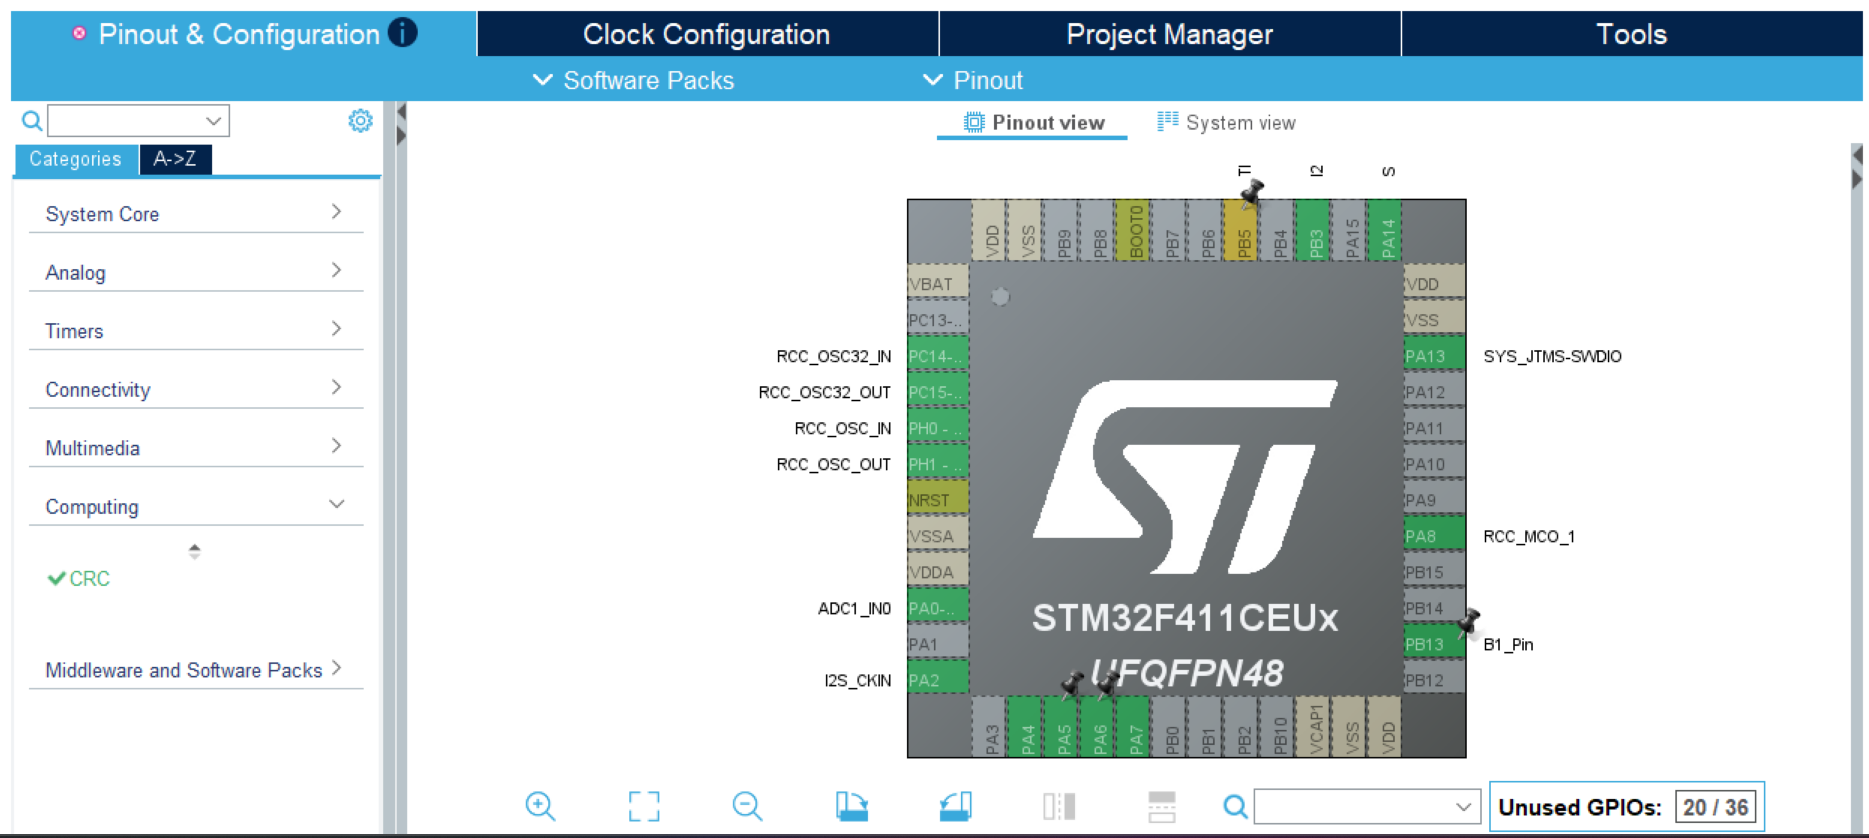
\includegraphics[width=0.8\linewidth]{imagens/Pinout_Configuration.png}
    \caption{Visão geral da aba Pinout \& Configuration mostrando as categorias de periféricos e o diagrama do microcontrolador.}
    \label{fig:pinout_config}
\end{figure}

A tela é dividida em duas lógicas principais:
\begin{itemize}
    \item \textbf{Menu de Categorias (Esquerda):} Agrupa os recursos internos do chip. Você encontra os módulos divididos por função, como \textit{System Core} (onde ficam o RCC, SYS e DMA), \textit{Analog} (ADC), \textit{Timers}, e \textit{Connectivity} (I2C, SPI, USART). É aqui que você ``liga'' um periférico para que o CubeMX reserve os recursos de memória para ele.
    \item \textbf{Visão do Chip (Centro):} Mostra o encapsulamento físico do seu microcontrolador (no caso, um STM32F411CEUx de 48 pinos). As cores dos pinos informam o estado do hardware:
    \begin{itemize}
        \item \textbf{Cinza:} Pino não utilizado, em estado de alta impedância.
        \item \textbf{Verde:} Pino configurado e funcional (Ex: Pinos PA13 e PA14 alocados para o SWDIO e SWCLK).
        \item \textbf{Amarelo:} Pinos dedicados a funções de sistema ou alimentação que não podem ser alterados livremente pelo usuário (Ex: Pino BOOT0).
    \end{itemize}
\end{itemize}

\subsubsection{Categorias de Periféricos (O Menu Lateral)}
Na lateral esquerda da aba de Pinout, o CubeMX organiza todos os blocos de silício disponíveis no seu chip em categorias lógicas. Quando você clica em um item e altera seu estado (ex: de \textit{Disable} para \textit{Half-Duplex}), o software automaticamente reserva os pinos físicos na imagem central e acende as caixas de configuração.

As quatro primeiras categorias são a base de 90\% dos projetos de sistemas embarcados e merecem uma atenção minuciosa:

\textbf{1. System Core (O Núcleo do Sistema)}\\
Aqui estão os órgãos vitais que mantêm o chip vivo e rodando. Diferente de um sensor externo, você sempre precisará configurar itens desta lista:
\begin{itemize}
    \item \textbf{RCC (Reset and Clock Control):} É onde você avisa ao chip se os relógios (HSE e LSE) virão de osciladores internos (imprecisos) ou de cristais de quartzo externos (alta precisão).
    \item \textbf{SYS (System):} Contém a configuração da base de tempo da HAL (geralmente o SysTick) e, mais criticamente, o \textbf{Debug}. Se você esquecer de habilitar o \textit{Serial Wire} (SWD) aqui, ao gravar o código pela primeira vez, os pinos de depuração serão desativados e você ``trancará'' a sua placa, impedindo futuras gravações com o ST-Link.
    \item \textbf{GPIO:} Um painel centralizado para ver e alterar o estado de todos os pinos de entrada e saída (Push-Pull, Pull-Up/Down, velocidade de transição).
    \item \textbf{NVIC:} O painel de controle de Interrupções. É aqui que você define as prioridades de quem pode interromper o código principal.
    \item \textbf{DMA (Direct Memory Access):} Permite configurar canais para que os periféricos joguem dados direto na memória RAM sem incomodar o processador.
\end{itemize}

\textbf{2. Analog (O Mundo Físico)}\\
O processador só entende 0 e 1, mas o mundo real é contínuo. Esta categoria lida com sinais elétricos brutos.
\begin{itemize}
    \item \textbf{ADC (Analog-to-Digital Converter):} Transforma variações de voltagem (como a leitura de um termistor, potenciômetro ou sensor de pressão analógico) em números digitais (0 a 4095, no caso de 12 bits). Aqui você habilita os canais do multiplexador para ler vários pinos simultaneamente.
\end{itemize}
\textit{(Nota: Dependendo do modelo do STM32, você também encontraria aqui o DAC para converter sinais digitais de volta em áudio ou ondas analógicas, e Amplificadores Operacionais embutidos).}

\textbf{3. Timers (O Controle do Tempo)}\\
Tudo que exige ritmo, contagem ou agendamento está aqui.
\begin{itemize}
    \item \textbf{RTC (Real-Time Clock):} O calendário e relógio isolado com domínio de energia próprio (VBAT).
    \item \textbf{Advanced Timers (Ex: TIM1):} Timers parrudões com recursos específicos para controle de motores trifásicos e inserção de \textit{Dead-Time} (para não queimar pontes H).
    \item \textbf{General Purpose Timers (Ex: TIM2 a TIM5):} Onde você vai gerar a maioria dos seus sinais PWM para servos motores e LEDs, ou medir a frequência de sinais externos (Input Capture).
    \item \textbf{Watchdog (IWDG e WWDG):} Os temporizadores de segurança que resetam o chip caso o seu código trave em um loop infinito.
\end{itemize}

\textbf{4. Connectivity (As Vias de Comunicação)}\\
Aqui é onde o seu microcontrolador ganha a capacidade de conversar com o mundo externo, seja com outros chips na mesma placa ou com computadores.
\begin{itemize}
    \item \textbf{I2C e SPI:} Para comunicação rápida com sensores (giroscópios, barômetros, memórias Flash, displays OLED).
    \item \textbf{USART / UART:} Para telemetria via rádio, módulos GPS, Bluetooth ou para mandar mensagens de \texttt{printf} para o terminal serial do computador.
    \item \textbf{USB\_OTG\_FS:} Permite que o STM32 se comporte como um dispositivo USB real (como um pendrive ou um mouse) para o Windows/Linux.
\end{itemize}

\textbf{Outras Categorias Avançadas:}
\begin{itemize}
    \item \textbf{Computing:} Contém aceleradores matemáticos embutidos no silício. No STM32F411, a ferramenta principal aqui é o \textbf{CRC} (Cyclic Redundancy Check), um hardware dedicado a calcular rapidamente códigos de verificação para garantir que dados recebidos por rádio ou memórias não estejam corrompidos.
    \item \textbf{Middleware and Software Packs:} Diferente do resto, isso não é silício, mas sim código pré-pronto de alto nível que a ST injeta no seu projeto. Aqui você pode habilitar o \textbf{FreeRTOS} (um sistema operacional em tempo real de nível aeroespacial e automotivo), o \textbf{FatFS} (para o chip entender como ler pastas e arquivos em um cartão SD), e bibliotecas completas de USB (USB Device Library).
\end{itemize}

\subsection{Clock Configuration (A Árvore de Frequências)}
Esta aba exibe a arquitetura completa do sistema de relógios, desde os cristais externos (HSE/LSE) até os multiplicadores PLL e barramentos APB1/APB2.
\textit{Nota: A explicação matemática e arquitetural detalhada do roteamento de energia e frequência encontra-se na seção \textbf{The Clock \& Timers} deste manual.}

\subsection{Project Manager (A Geração de Código)}
Depois de configurar o hardware, esta aba dita como o código fonte será estruturado no seu disco rígido.

\begin{figure}[H]
    \centering
    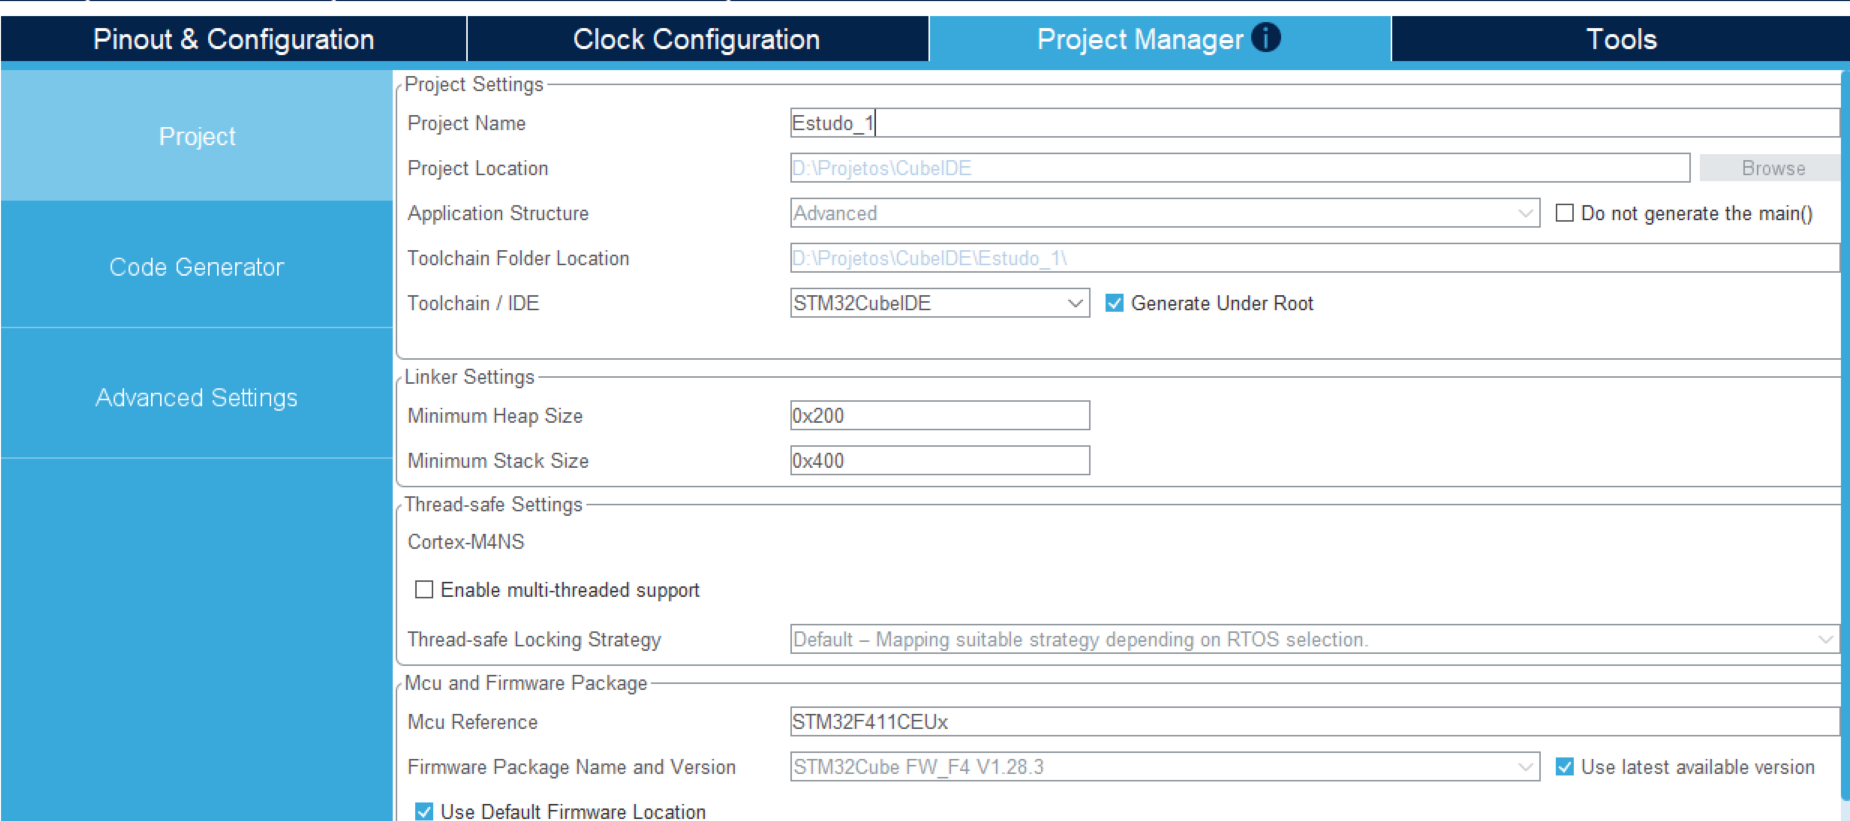
\includegraphics[width=0.8\linewidth]{imagens/Project_Manager.png}
    \caption{Configurações do Project Manager, definindo a Toolchain e o tamanho da memória.}
    \label{fig:project_manager}
\end{figure}

No submenu \textbf{Project}, as definições críticas incluem:
\begin{itemize}
    \item \textbf{Toolchain / IDE:} É obrigatório selecionar a IDE que fará a compilação. Para o nosso fluxo, deve estar configurado como \textbf{STM32CubeIDE}.
    \item \textbf{Linker Settings:} Define o espaço mínimo reservado na memória RAM para operações dinâmicas. Por padrão, o CubeMX aloca \texttt{0x200} (512 bytes) para o \textit{Heap} (alocação dinâmica como \texttt{malloc}) e \texttt{0x400} (1024 bytes) para o \textit{Stack} (pilha de execução de funções e variáveis locais). Em projetos com FreeRTOS ou bibliotecas pesadas, esses valores precisam ser aumentados.
    \item \textbf{Mcu and Firmware Package:} Mostra a versão exata da biblioteca HAL que será injetada no projeto (ex: STM32Cube FW\_F4 V1.28.3).
\end{itemize}

\textit{(Dica Prática: No submenu lateral \textbf{Code Generator}, é uma excelente prática marcar a opção de ``Gerar arquivos .c/.h separados por periférico'', o que evita que o arquivo \texttt{main.c} fique com milhares de linhas de inicialização aglomeradas).}

\subsection{Tools (Ferramentas de Análise)}
A aba \textit{Tools} contém utilitários de engenharia que auxiliam no planejamento antes de a placa física existir.

\begin{figure}[H]
    \centering
    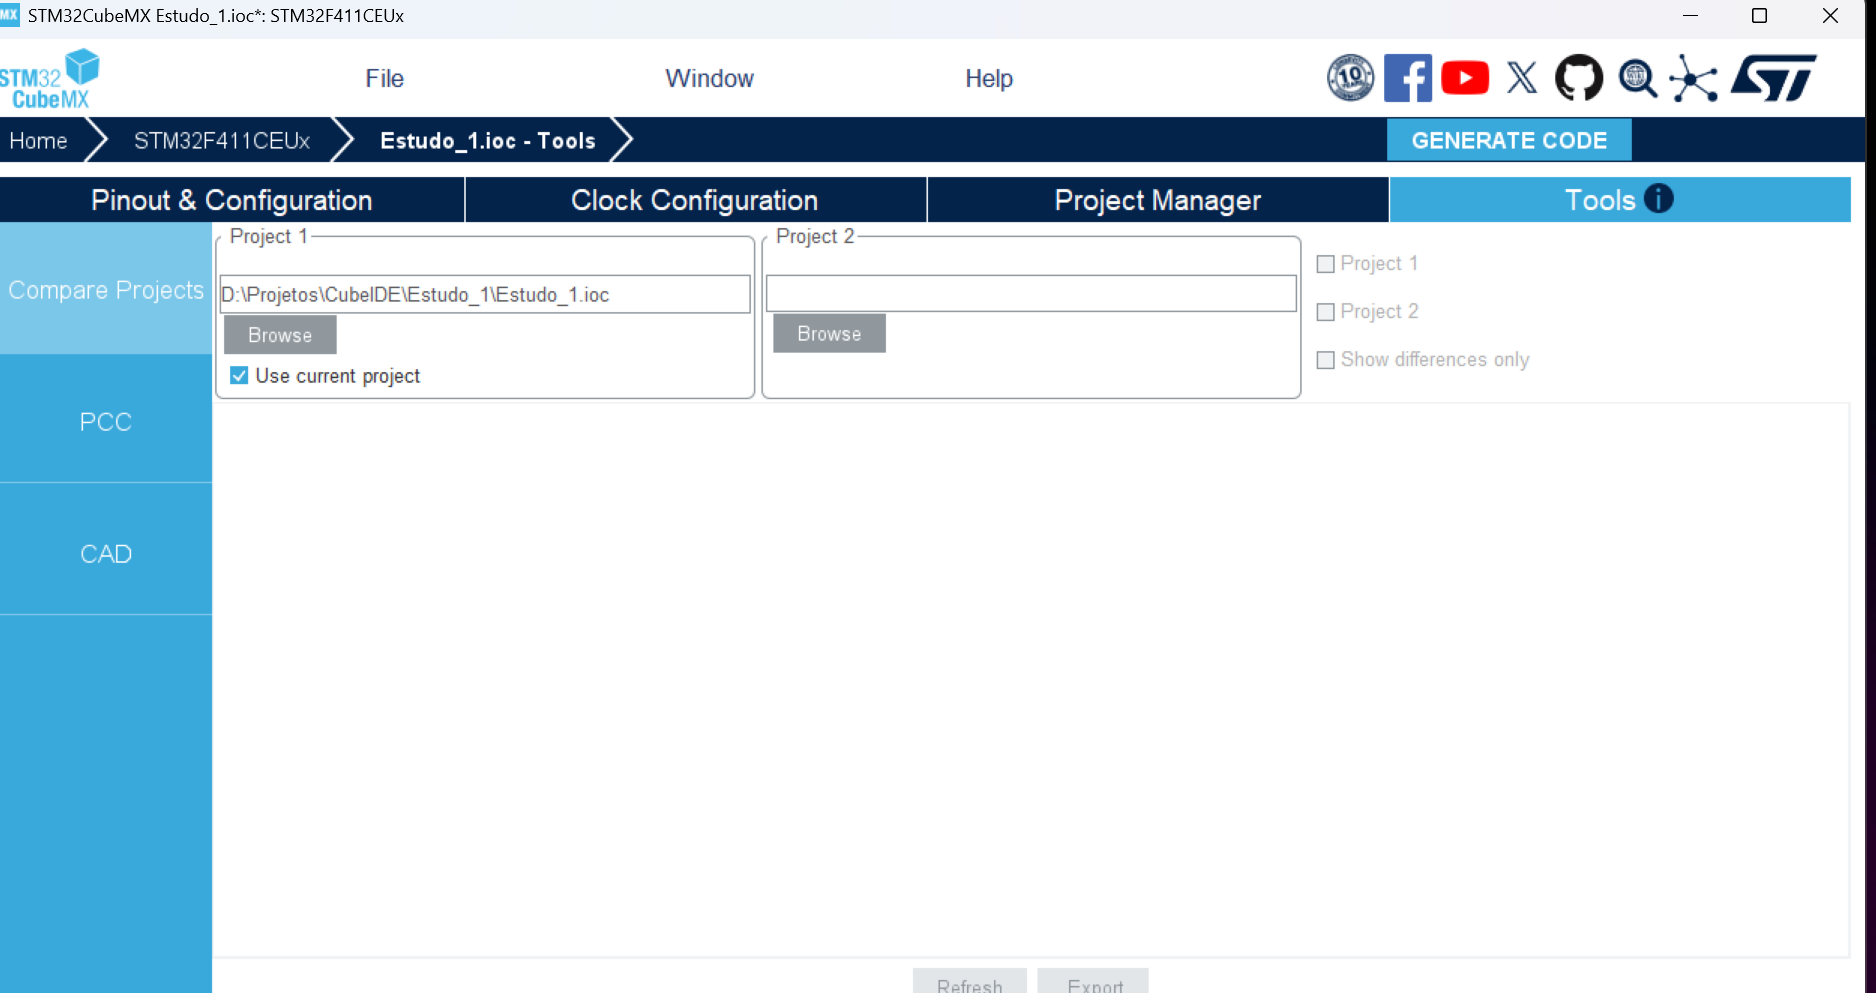
\includegraphics[width=0.8\linewidth]{imagens/Tools.png}
    \caption{Aba Tools com acesso ao calculador de consumo e comparação de projetos.}
    \label{fig:tools}
\end{figure}

\begin{itemize}
    \item \textbf{PCC (Power Consumption Calculator):} É a ferramenta mais importante desta aba. Ela permite simular o consumo de bateria do foguete ou satélite. Você insere qual bateria vai usar e define as etapas de voo (ex: ``5 minutos em modo Run a 96 MHz, depois 2 horas em Deep Sleep''). O software cruza isso com o datasheet e gera gráficos mostrando quantos miliamperes o chip vai drenar.
    \item \textbf{Compare Projects e CAD:} Permite comparar o arquivo atual \texttt{.ioc} com revisões anteriores para ver o que mudou na configuração de hardware, além de opções de exportação para ferramentas de design de PCB.
\end{itemize}

% ==========================================
% COMPILAÇÃO E DEPURAÇÃO
% ==========================================
\section{Compilação e Depuração}

\begin{figure}[H]
    \centering
    
\includegraphics[width=0.8\linewidth]{imagens/Compilation_and_Debugging.png}
    \caption{Compilation and Debugging}
    \label{fig:compilation}
\end{figure}

Escrever o código em C é apenas a primeira etapa. Em um computador normal, o sistema operacional carrega o seu programa na memória RAM e o executa. Em um microcontrolador, o seu código precisa ser transformado em sinais elétricos permanentes gravados na memória Flash do chip, e a própria inicialização da memória RAM deve ser feita manualmente pelo hardware antes do \texttt{main()} começar.

\subsection{A Toolchain (O Caminho do Código)}
Quando você clica no botão de ``Build'' (o martelinho no STM32CubeIDE), uma engrenagem chamada \textbf{Toolchain} (geralmente o GCC ARM Embedded) entra em ação em três etapas:



\begin{enumerate}
    \item \textbf{Compilador (gcc):} Traduz os seus arquivos \texttt{.c} para a linguagem de máquina específica do núcleo ARM Cortex-M4 (arquitetura Thumb-2).
    \item \textbf{Assembler (as):} Converte as instruções em linguagem de montagem (Assembly) para os códigos binários brutos (os zeros e uns) em arquivos objeto (\texttt{.o}).
    \item \textbf{Linker (ld):} É a peça mais importante no mundo embarcado. Ele pega todos os seus arquivos soltos (o seu \texttt{main.o}, o seu driver \texttt{bmp180.o} e as bibliotecas da HAL) e os ``costura'' em um único arquivo final (\texttt{.elf} ou \texttt{.bin}).
\end{enumerate}

\textbf{O Linker Script (.ld):}\\
Para que o Linker consiga costurar o código, ele precisa do mapa do tesouro. O arquivo Linker Script (ex: \texttt{STM32F411CEUX\_FLASH.ld}) diz ao compilador exatamente onde as coisas devem ficar fisicamente no chip:
\begin{itemize}
    \item \textbf{.text:} Onde ficam as instruções do seu código e as constantes (como \texttt{const int x = 5;}). Isso vai direto para a memória Flash (não apaga quando desliga a energia).
    \item \textbf{.data:} Variáveis globais inicializadas (ex: \texttt{int temperatura = 25;}).
    \item \textbf{.bss:} Variáveis globais não inicializadas (ex: \texttt{int buffer[100];}). O Linker sabe que essas precisam ir para a RAM.
\end{itemize}

\subsection{O Arquivo de Startup (O que acontece antes do main)}
Se você olhar a sua pasta de projeto, verá um arquivo escrito em Assembly chamado \texttt{startup\_stm32f411retx.s}. Ele é o verdadeiro início do seu sistema, executado no milissegundo em que o chip recebe energia.
Ele faz o trabalho sujo que um Sistema Operacional faria:
\begin{itemize}
    \item Configura o Stack Pointer (ponteiro da pilha de memória).
    \item Copia as variáveis da seção \texttt{.data} da Flash para a RAM.
    \item Preenche a seção \texttt{.bss} da RAM com zeros.
    \item Chama a função \texttt{SystemInit()} para ligar o clock básico.
    \item Só então, ele faz a chamada para o seu \texttt{main()}.
\end{itemize}

\subsection{Depuração em Hardware (O Poder do SWD)}
Diferente do Arduino, onde você tenta achar erros enchendo o código de \texttt{Serial.print()}, a arquitetura ARM possui um hardware dedicado dentro do chip só para espionar a CPU.

A interface \textbf{SWD} (\textit{Serial Wire Debug}) usa apenas 2 pinos (SWDIO para dados e SWCLK para clock) para conectar o seu chip ao gravador ST-Link. Com isso, você ganha acesso absoluto ao núcleo do processador em tempo real.

\textbf{Ferramentas de Debug no CubeIDE:}
\begin{itemize}
    \item \textbf{Breakpoints:} Você pode clicar na lateral do código e mandar a CPU parar fisicamente a execução naquela linha exata. Os motores do foguete continuam ligados, mas a execução do código congela para você analisar as variáveis.
    \item \textbf{Step Into / Step Over:} Permite avançar o código linha por linha, vendo como a matemática se comporta a cada ciclo.
    \item \textbf{A Visão de Registradores (SFRs):} O Santo Graal do Bare-Metal. O CubeIDE tem uma aba chamada \textit{SFRs (Special Function Registers)}. Lá, você pode ver os registradores do RCC, SPI, I2C e GPIO mudando de 0 para 1 em tempo real. Se o seu SPI não está funcionando, você pausa o código, abre o SFR e verifica se o bit \texttt{SPE} do registrador \texttt{CR1} realmente está em 1.
\end{itemize}

\subsection{O Terror do Embarcado: O Hard Fault}
Se você tentar acessar uma memória que não existe, dividir um número por zero, ou tentar escrever em um periférico cujo Clock não foi ligado no RCC, o núcleo ARM dispara uma exceção gravíssima chamada \textbf{Hard Fault}.

Quando isso acontece, o microcontrolador aborta o seu código e pula para um loop infinito de segurança chamado \texttt{HardFault\_Handler()}, localizado no arquivo \texttt{stm32f4xx\_it.c}. O chip ``trava'' de propósito.

Na depuração, se o seu código travou, você aperta o botão de ``Pause'', olha a janela \textit{Call Stack} (Pilha de Chamadas) e consegue rastrear exatamente qual função e qual linha do seu \texttt{.c} gerou a falha catastrófica.

\subsection{Gravando sem ST-Link (Bootloader via USB-C e UART)}
O SWD é a ferramenta definitiva para depuração na bancada, mas e quando a placa de aviônica já está montada, encapsulada e os pinos SWD estão inacessíveis? Em projetos de foguetemodelismo, é comum deixar apenas uma porta USB-C ou um conector serial exposto como um ``cordão umbilical'' para atualizar o firmware diretamente na base de lançamento.

A STMicroelectronics previu isso e gravou um software inalterável direto no silício de todo STM32, chamado \textbf{System Memory Bootloader}.
Esse Bootloader de fábrica sabe ler códigos binários chegando pelas portas UART, I2C, SPI e, principalmente, pelo USB nativo do chip. Para ativá-lo, você não precisa de nenhum gravador externo, apenas de uma configuração física nos pinos de Boot.



\textbf{A Chave Mestra: O Pino BOOT0}\\
No momento exato em que o STM32 recebe energia (ou quando o botão de Reset é solto), o hardware lê o estado do pino BOOT0.
\begin{itemize}
    \item \textbf{BOOT0 em LOW (0V - Padrão):} O chip aponta para a memória Flash e roda o seu código \texttt{main.c} normalmente.
    \item \textbf{BOOT0 em HIGH (3.3V):} O chip ignora a sua memória Flash e entra no modo Bootloader da ST. Ele congela e fica escutando as portas de comunicação esperando você enviar um novo código.
\end{itemize}

Existem duas formas principais de aproveitar isso na prática:

\textbf{1. O Método USB-C (DFU - Device Firmware Upgrade)}\\
Se você estiver usando uma placa como a Black Pill (STM32F411), a porta USB-C dela já está ligada diretamente aos pinos de dados USB do chip (PA11 e PA12). Para gravar o código usando apenas um cabo USB de celular espetado no computador:
\begin{enumerate}
    \item Pressione e segure o botão BOOT0 na placa.
    \item Dê um clique no botão NRST (Reset).
    \item Solte o botão BOOT0.
\end{enumerate}
Isso coloca o chip em modo DFU. No computador, você usa o software oficial \textit{STM32CubeProgrammer}. 
Basta selecionar a conexão via ``USB'', apontar para o seu arquivo \texttt{.elf} ou \texttt{.bin} (gerado na pasta Debug da IDE) e clicar em \textit{Download}. O código é gravado na Flash instantaneamente.

\textbf{2. O Método UART (Conversor USB-Serial)}\\
Se a sua placa customizada não tiver um conector USB, você pode gravar o código usando os mesmos pinos TX e RX que configuramos na Seção de UART. Você precisará de um conversor USB-TTL barato (como o FT232RL ou CP2102).
\begin{enumerate}
    \item Ligue o TX do conversor no pino RX do STM32 (ex: PA10 / USART1).
    \item Ligue o RX do conversor no pino TX do STM32 (ex: PA9 / USART1).
    \item Ligue o GND de ambos.
    \item Com a placa desligada, feche um jumper ligando o pino BOOT0 no 3.3V.
    \item Ligue a placa (ou dê um Reset).
\end{enumerate}
No \textit{STM32CubeProgrammer}, você seleciona a conexão ``UART'', escolhe a porta COM do conversor e faz o envio do arquivo. Quando terminar de gravar, você deve remover o jumper do BOOT0 (voltando ele para 0V) e dar um Reset na placa para que o seu novo código comece a rodar.

\textbf{Atenção à Restrição do Bootloader:} Embora gravar por USB-C ou UART seja extremamente prático e barato, nenhum desses métodos permite depuração (Debug). Você só consegue enviar o código. Se precisar usar Breakpoints ou ler os registradores em tempo real, você é fisicamente obrigado a usar os pinos SWD com um ST-Link.

% ==========================================
% ANEXOS
% ==========================================
\newpage
\section*{Anexos}
\label{anexos}
\addcontentsline{toc}{section}{Anexos}

\begin{figure}[H]
    \centering
    
\includegraphics[width=0.6\linewidth]{imagens/Anexos.png}
    \caption{Anexos}
    \label{fig:anexos}
\end{figure}

% ==========================================
% ANEXO 1: BITWISE OPERATIONS
% ==========================================
\subsection*{Anexo 1: Bitwise Operations}
\label{anexo:1}
\addcontentsline{toc}{subsection}{Anexo 1: Bitwise Operations}

As operações bitwise manipulam bits individuais dentro de um byte ou palavra, independentemente do valor decimal total.

\subsubsection*{1. Tabela Resumo dos Operadores}
\begin{table}[H]
    \centering
    \begin{tabular}{llcl}
    \toprule
    \textbf{Operador} & \textbf{Nome} & \textbf{Símbolo} & \textbf{Lógica Resumida} \\
    \midrule
    AND & E (Bit a Bit) & \texttt{\&} & Verdadeiro apenas se ambos forem 1. \\
    OR & OU (Inclusivo) & \texttt{|} & Verdadeiro se pelo menos um for 1. \\
    XOR & OU (Exclusivo) & \texttt{\^} & Verdadeiro se os bits forem diferentes. \\
    NOT & NÃO (Inversão) & \texttt{\~} & Inverte o valor (0 vira 1, 1 vira 0). \\
    Left Shift & Desloc. Esquerda & \texttt{<<} & Move bits para a esquerda (multiplica por 2). \\
    Right Shift & Desloc. Direita & \texttt{>>} & Move bits para a direita (divide por 2). \\
    \bottomrule
    \end{tabular}
\end{table}

\subsubsection*{2. Tabelas Verdade (Lógica Porta a Porta)}
Estas tabelas mostram o resultado bit a bit para todas as combinações possíveis de entrada (A e B).

\begin{table}[H]
    \centering
    \begin{tabular}{cc|c}
    \multicolumn{3}{c}{\textbf{Operação AND (\&)}} \\
    \toprule
    \textbf{Entrada A} & \textbf{Entrada B} & \textbf{Saída (A \& B)} \\
    \midrule
    0 & 0 & 0 \\
    1 & 0 & 0 \\
    0 & 1 & 0 \\
    1 & 1 & 1 \\
    \bottomrule
    \end{tabular}
    \quad
    \begin{tabular}{cc|c}
    \multicolumn{3}{c}{\textbf{Operação OR (|)}} \\
    \toprule
    \textbf{Entrada A} & \textbf{Entrada B} & \textbf{Saída (A | B)} \\
    \midrule
    0 & 0 & 0 \\
    1 & 0 & 1 \\
    0 & 1 & 1 \\
    1 & 1 & 1 \\
    \bottomrule
    \end{tabular}
\end{table}

\begin{table}[H]
    \centering
    \begin{tabular}{cc|c}
    \multicolumn{3}{c}{\textbf{Operação XOR (\textasciicircum)}} \\
    \toprule
    \textbf{Entrada A} & \textbf{Entrada B} & \textbf{Saída (A \textasciicircum\ B)} \\
    \midrule
    0 & 0 & 0 \\
    1 & 0 & 1 \\
    0 & 1 & 1 \\
    1 & 1 & 0 \\
    \bottomrule
    \end{tabular}
    \quad
    \begin{tabular}{c|c}
    \multicolumn{2}{c}{\textbf{Operação NOT (\textasciitilde)}} \\
    \toprule
    \textbf{Entrada A} & \textbf{Saída (\textasciitilde A)} \\
    \midrule
    0 & 1 \\
    1 & 0 \\
    - & - \\
    - & - \\
    \bottomrule
    \end{tabular}
\end{table}

\subsubsection*{3. Exemplos de Cálculo (Byte Completo)}
Para estes exemplos, considere: \texttt{A = 1010 1100} e \texttt{B = 0000 1111}.

\begin{table}[H]
    \centering
    % Trocamos o p{3cm} por 'l' (esquerda) para não justificar os espaços
    \begin{tabular}{l l p{6cm}}
    \toprule
    \textbf{Operação} & \textbf{Cálculo Binário} & \textbf{Explicação Visual} \\
    \midrule
    \textbf{AND (\&)} & 
    % Tabela aninhada para travar o alinhamento monoespaçado
    \begin{tabular}{@{}l@{}}
    \texttt{~~1010 1100} \\
    \texttt{\&~0000 1111} \\
    \texttt{=~0000 1100}
    \end{tabular} & 
    Mantém apenas os bits que são 1 em cima E em baixo. (Note os últimos 4 bits). \\
    \midrule
    \textbf{OR (|)} & 
    \begin{tabular}{@{}l@{}}
    \texttt{~~1010 1100} \\
    \texttt{|~0000 1111} \\
    \texttt{=~1010 1111}
    \end{tabular} & 
    Combina os bits. Se tiver 1 em cima OU em baixo, o resultado é 1. \\
    \midrule
    \textbf{XOR (\textasciicircum)} & 
    \begin{tabular}{@{}l@{}}
    \texttt{~~1010 1100} \\
    \texttt{\textasciicircum~0000 1111} \\
    \texttt{=~1010 0011}
    \end{tabular} & 
    Onde os bits são iguais (1 e 1 ou 0 e 0), vira 0. Onde são diferentes, vira 1. \\
    \bottomrule
    \end{tabular}
\end{table}

\subsubsection*{4. Operações de Deslocamento (Shift)}
Visualização do movimento dos bits. Zeros são inseridos para preencher o espaço vazio.

\textbf{Left Shift (<<)}\\
Deslocando o valor \texttt{0000 0011} (Decimal 3) duas casas para a esquerda.
\begin{table}[H]
    \centering
    \begin{tabular}{lccl}
    \toprule
    \textbf{Passo} & \textbf{Binário} & \textbf{Decimal} & \textbf{O que aconteceu} \\
    \midrule
    Original & \texttt{0000 0011} & 3 & Valor inicial. \\
    \texttt{<< 1} & \texttt{0000 0110} & 6 & Bits movem 1 casa. O 0 entra na direita. (3 * 2) \\
    \texttt{<< 2} & \texttt{0000 1100} & 12 & Bits movem mais 1 casa. (6 * 2) \\
    \bottomrule
    \end{tabular}
\end{table}

\textbf{Right Shift (>>)}\\
Deslocando o valor \texttt{1000 0000} (Decimal 128) duas casas para a direita.
\begin{table}[H]
    \centering
    \begin{tabular}{lccl}
    \toprule
    \textbf{Passo} & \textbf{Binário} & \textbf{Decimal} & \textbf{O que aconteceu} \\
    \midrule
    Original & \texttt{1000 0000} & 128 & Valor inicial. \\
    \texttt{>> 1} & \texttt{0100 0000} & 64 & Bits movem 1 casa. O 0 entra na esquerda. (128 / 2) \\
    \texttt{>> 2} & \texttt{0010 0000} & 32 & Bits movem mais 1 casa. (64 / 2) \\
    \bottomrule
    \end{tabular}
\end{table}

% ==========================================
% ANEXO 2: FPU (Floating Point Unit)
% ==========================================
\subsection*{Anexo 2: FPU (Floating Point Unit)}
\label{anexo:2}
\addcontentsline{toc}{subsection}{Anexo 2: FPU (Floating Point Unit)}

\begin{table}[H]
    \centering
    \resizebox{\textwidth}{!}{%
    \begin{tabular}{lllll}
    \toprule
    \textbf{Unidade} & \textbf{Tipos (C/C++)} & \textbf{Padrão Matemático} & \textbf{Performance} & \textbf{Observação Crítica} \\
    \midrule
    \textbf{ALU (CPU)} & int, int32\_t & Comp. de Dois & 1 ciclo (Nativo) & Usado para loops e lógica booleana. \\
    \textbf{ALU (CPU)} & int64\_t & Comp. de Dois & $\sim$2 a 12 ciclos & O compilador quebra a operação em duas. \\
    \textbf{FPU (Single)} & float & IEEE 754 (32 bits) & 1 a 3 ciclos & Usar sufixo f e flag \texttt{-mfloat-abi=hard}. \\
    \textbf{ALU (Soft)} & double & IEEE 754 (64 bits) & $\sim$50 a 100+ ciclos & Gargalo: Calculado via software no F4. \\
    \textbf{FPU (Double)} & double & IEEE 754 (64 bits) & 1 a 3 ciclos & Apenas STM32F7/H7 possuem DP-FPU. \\
    \bottomrule
    \end{tabular}}
\end{table}

\textbf{Flag do Compilador: \texttt{-mfloat-abi}}
\begin{table}[H]
    \centering
    \begin{tabular}{lp{6cm}p{6cm}}
    \toprule
    \textbf{Opção} & \textbf{O que acontece?} & \textbf{Performance / Compatibilidade} \\
    \midrule
    \texttt{soft} & Ignora a FPU. Tudo é calculado pela ALU via software. & Péssima para floats. Compatível com qualquer lib. \\
    \texttt{softfp} & Usa a FPU para calcular, mas passa parâmetros nos registradores da CPU. & Média (Gargalo na cópia de dados). \\
    \texttt{hard} & Usa a FPU para calcular e passar parâmetros. & Máxima. Sem overhead. Só linka com bibliotecas também compiladas em \texttt{hard}. \\
    \bottomrule
    \end{tabular}
\end{table}

% ==========================================
% ANEXO 3: Modes e Pulls do GPIO
% ==========================================
\subsection*{Anexo 3: Modes e Pulls do GPIO}
\label{anexo:3}
\addcontentsline{toc}{subsection}{Anexo 3: Modes e Pulls do GPIO}

\begin{figure}[H]
    \centering
    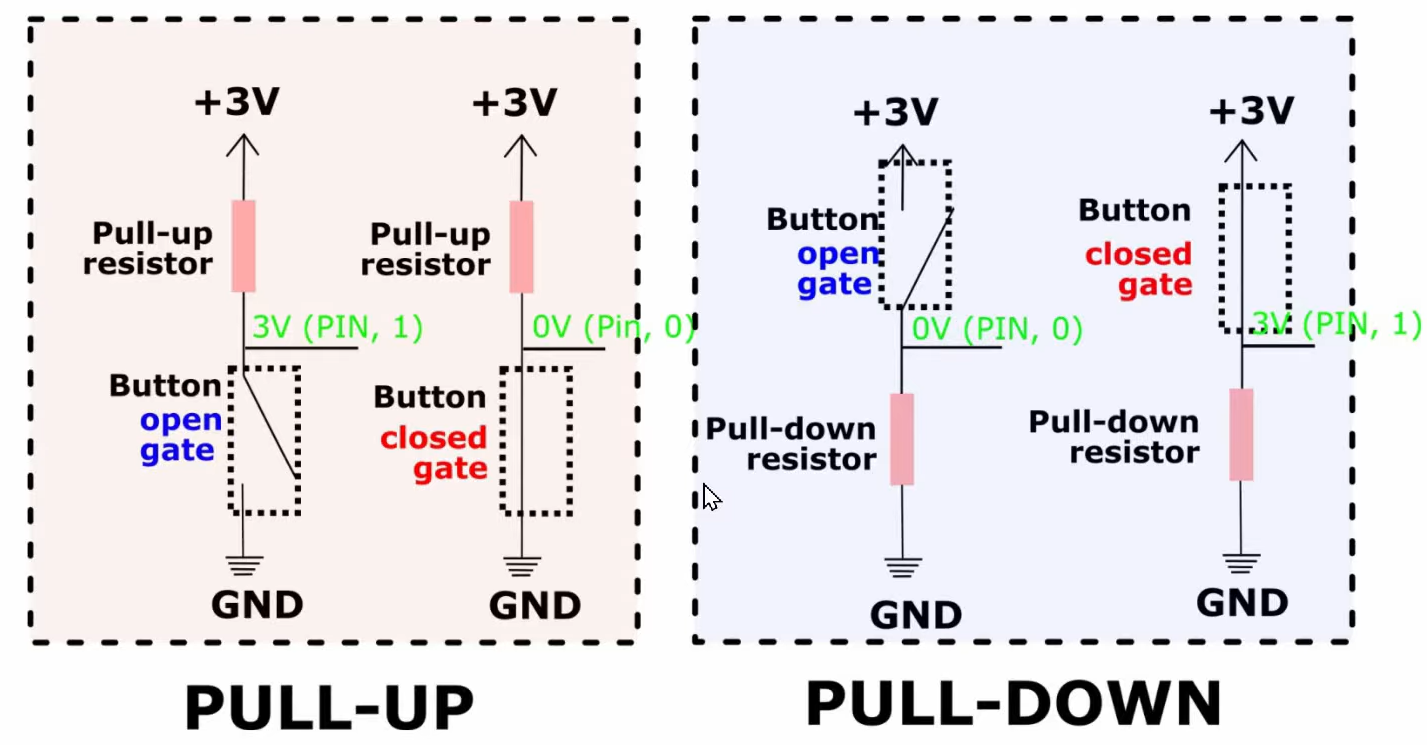
\includegraphics[width=0.8\linewidth]{imagens/Up_down.png}
    \caption{Pull-Up and Pull-Down}
    \label{fig:pull_up_down}
\end{figure}

\subsubsection*{1. Por que o botão não teve \texttt{WritePin (HIGH)}?}
O Mode escolhe qual ferramenta você vai usar.

\vspace{0.3cm}
\noindent\textbf{A. Módulos de ENTRADA (Input)}\\
\textbf{\texttt{GPIO\_MODE\_INPUT}} (Floating - Flutuante)
\begin{itemize}
    \item \textbf{O que é:} O pino fica em alta impedância (Hi-Z). É como se o fio estivesse solto dentro do chip.
    \item \textbf{Uso:} Quando o sensor externo já manda 0V e 3.3V fortes por conta própria.
    \item \textbf{Perigo:} Se nada estiver conectado, o pino vira uma antena e lê valores aleatórios (ruído).
\end{itemize}

\textbf{\texttt{GPIO\_MODE\_INPUT} com \texttt{GPIO\_PULLUP}}
\begin{itemize}
    \item \textbf{O que é:} Um resistor interno fraco conecta o pino ao 3.3V.
    \item \textbf{Estado padrão:} 1 (HIGH).
    \item \textbf{Uso:} Botões que conectam ao GND quando apertados. (Lógica invertida: apertou = 0).
\end{itemize}

\textbf{\texttt{GPIO\_MODE\_INPUT} com \texttt{GPIO\_PULLDOWN}}
\begin{itemize}
    \item \textbf{O que é:} Um resistor interno fraco conecta o pino ao GND (0V).
    \item \textbf{Estado padrão:} 0 (LOW).
    \item \textbf{Uso:} Botões que conectam ao 3.3V quando apertados. (Lógica direta: apertou = 1).
\end{itemize}

\textbf{\texttt{GPIO\_MODE\_ANALOG}}
\begin{itemize}
    \item \textbf{O que é:} Desliga TUDO. Desliga até o ``Schmidt Trigger'' (o circuito digital que decide se é 0 ou 1). O pino fica conectado direto ao conversor ADC.
    \item \textbf{Uso:} Ler voltagens variáveis (ex: potenciômetro, sensor de temperatura).
    \item \textbf{Importante:} É o modo que menos gasta energia, pois desliga a parte digital do pino.
\end{itemize}

\vspace{0.3cm}
\noindent\textbf{B. Módulos de SAÍDA (Output)}\\
Aqui está a maior confusão da maioria dos programadores: Push-Pull vs Open-Drain.

\textbf{\texttt{GPIO\_MODE\_OUTPUT\_PP}} (Push-Pull - Empurra e Puxa)
\begin{itemize}
    \item \textbf{Como funciona:} O chip tem dois transistores. Um liga no 3.3V e outro no GND. O pino sempre tem tensão definida.
    \item \textbf{Uso:} Acender LEDs, comunicar com outros chips rápidos (SPI, displays).
    \item \textbf{Analogia:} Você segura uma porta com as duas mãos. Você pode empurrar ela para abrir ou puxar para fechar com força.
\end{itemize}

\textbf{\texttt{GPIO\_MODE\_OUTPUT\_OD}} (Open-Drain - Dreno Aberto)
\begin{itemize}
    \item \textbf{Como funciona:} O chip só tem o transistor de baixo (GND). O de cima (3.3V) não existe ou fica desligado.
    \item \textbf{Se escrever 0:} O pino conecta ao GND (Terra forte).
    \item \textbf{Se escrever 1:} O pino fica Flutuante (Desconectado).
    \item \textbf{Para funcionar:} Você PRECISA de um resistor de Pull-Up externo (ou ativar o interno).
    \item \textbf{Uso Principal:} Protocolo I2C. \textit{Por que?} Vários chips podem estar no mesmo fio. Se um mandar 0V e o outro mandar 3.3V (Push-Pull), dá curto-circuito. No Open-Drain, se um manda 0V e o outro ``não faz nada'' (1), ninguém queima. É como uma linha de ônibus onde qualquer um pode puxar a corda para parar.
    \item \textbf{Uso Secundário:} Controlar dispositivos de 5V com um chip de 3.3V (se o pino for ``5V Tolerant''). O pino aterra o circuito de 5V sem injetar 3.3V nele.
\end{itemize}

\vspace{0.3cm}
\noindent\textbf{C. Funções Alternadas (AF)}\\
\textbf{\texttt{GPIO\_MODE\_AF\_PP} e \texttt{GPIO\_MODE\_AF\_OD}}
\begin{itemize}
    \item \textbf{O que é:} Você entrega o controle do pino para um periférico interno (SPI, UART, Timer, I2C). O \texttt{HAL\_GPIO\_WritePin} para de funcionar nesse pino.
    \item \textbf{Exemplo:} O pino TX da UART precisa ser \texttt{AF\_PP} (Push-Pull controlado pelo hardware da UART). O pino SDA do I2C precisa ser \texttt{AF\_OD} (Open-Drain controlado pelo hardware do I2C).
\end{itemize}

% ==========================================
% ANEXO 4: ODR vs. BSSR
% ==========================================
\subsection*{Anexo 4: ODR vs. BSRR}
\label{anexo:4}
\addcontentsline{toc}{subsection}{Anexo 4: ODR vs. BSRR}

\subsubsection*{1. O Perigo do ODR: Read-Modify-Write (RMW)}
Quando você quer mudar apenas um pino usando o registrador ODR (como \texttt{GPIOA->ODR |= (1 << 5)}), o processador não consegue mudar apenas um bit magicamente. Ele precisa seguir 3 passos (conhecido como RMW):
\begin{enumerate}
    \item \textbf{Read:} O processador lê o valor atual de toda a porta A (todos os 16 pinos) para um registrador interno.
    \item \textbf{Modify:} Ele altera o bit 5 dentro desse registrador interno.
    \item \textbf{Write:} Ele escreve o valor completo (modificado) de volta no ODR.
\end{enumerate}

\textbf{O Risco (Condição de Corrida):}
Imagine que você está no Passo 2 (modificando o bit do LED). De repente, ocorre uma Interrupção! A interrupção muda o estado de outro pino (ex: Pino 6) na mesma porta. Quando a interrupção termina, o processador volta para o Passo 3 e escreve o valor antigo que ele tinha lido antes da interrupção. \textbf{Resultado:} A mudança feita pela interrupção no Pino 6 é sobrescrita e perdida. Você corrompeu o estado do outro pino sem querer.

\subsubsection*{2. A Mágica do BSRR: Operação Atômica}
O BSRR é um registrador especial ``Write-Only''.
\begin{itemize}
    \item Se você escreve 1 num bit, ele executa a ação (Set ou Reset).
    \item Se você escreve 0 num bit, ele não faz nada.
\end{itemize}
Por causa disso, você não precisa ler o estado anterior da porta. Você apenas envia o comando: ``Alterar Pino 5''.
\begin{lstlisting}[language=C]
GPIOA->BSRR = (1 << 5); // Apenas o bit 5 e 1. Os outros sao 0.
\end{lstlisting}
Como os 0s são ignorados pelo hardware do BSRR, os outros pinos não são tocados. Isso acontece em um único ciclo de clock. Não há risco de uma interrupção atrapalhar o processo, pois é uma \textbf{operação atômica} (indivisível).

\subsubsection*{Resumo da Comparação}
\begin{table}[H]
    \centering
    \resizebox{\textwidth}{!}{%
    \begin{tabular}{p{3.5cm}p{5cm}p{5cm}}
    \toprule
    \textbf{Característica} & \textbf{BSRR (Bit Set/Reset Register)} & \textbf{ODR (Output Data Register)} \\
    \midrule
    \textbf{Tipo de Operação} & Atômica (Indivisível). O hardware executa em um único ciclo. & Read-Modify-Write (RMW). O processador precisa ler, alterar e escrever. \\
    \midrule
    \textbf{Segurança} & \textbf{Total.} Imune a interrupções. & \textbf{Risco Crítico.} O estado de outros pinos da porta pode ser corrompido. \\
    \midrule
    \textbf{Velocidade} & \textbf{Alta.} Apenas 1 instrução. & \textbf{Média.} Requer múltiplas instruções. \\
    \midrule
    \textbf{Lógica de Escrita} & \textbf{Seletiva.} Escrever 1 atua, escrever 0 ignora. & \textbf{Absoluta.} O valor escrito substitui todo o estado da porta. \\
    \midrule
    \textbf{Uso Recomendado} & Sempre, para ligar/desligar pinos individuais em tempo de execução. & Apenas para ler o estado atual ou escrever na porta inteira de uma vez. \\
    \bottomrule
    \end{tabular}}
\end{table}

% ==========================================
% ANEXO 5: NVIC Bare-Metal Programming
% ==========================================
\subsection*{Anexo 5: NVIC Bare-Metal Programming}
\label{anexo:5}
\addcontentsline{toc}{subsection}{Anexo 5: NVIC Bare-Metal Programming}

\begin{figure}[H]
    \centering
    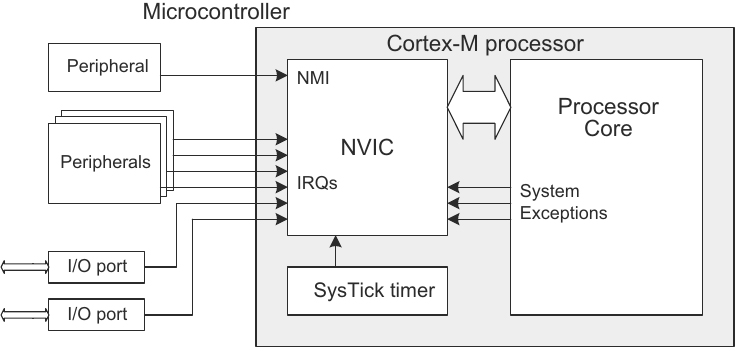
\includegraphics[width=0.8\linewidth]{imagens/NVIC.jpg}
    \caption{NVIC}
    \label{fig:nvic}
\end{figure}

\href{https://developer.arm.com/documentation/dui0553/latest/}{A documentação dos registradores NVIC} mostra as funções prontas do CMSIS e o que fazem:

\begin{figure}[H]
    \centering
    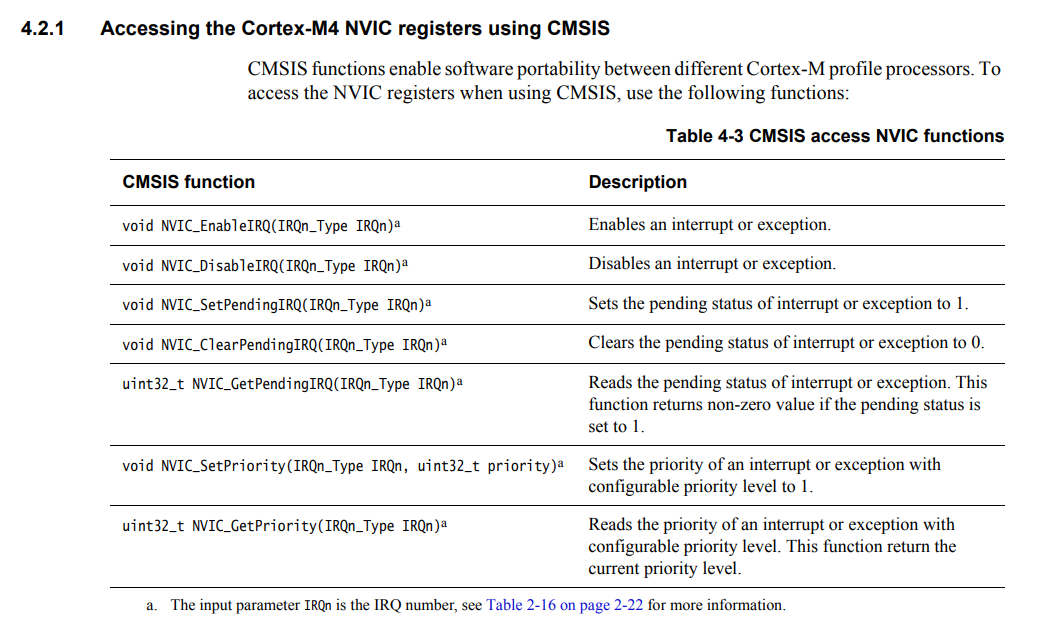
\includegraphics[width=0.8\linewidth]{imagens/NVIC_ARM.png}
    \caption{Documentação da ARM para o NVIC}
    \label{fig:nvic_arm}
\end{figure}

Agora como fazer o que o \texttt{NVIC\_SetPriority} e o \texttt{NVIC\_EnableIRQ} fazem? Comecemos:

Vamos usar o exemplo da interrupção \texttt{EXTI15\_10}, que no STM32F4 é mapeada para o canal (IRQ) número 40.

Eu joguei o número 40 no ar, mas no mundo Bare-Metal você nunca adivinha nada, tudo está rigorosamente mapeado e documentado. Esse número 40 é o \textit{Position} (ou IRQ Number) estipulado pela STMicroelectronics nos projetos da família STM32F4. Você encontra esse valor exato em dois lugares: no Manual do Hardware e no próprio Código C (CMSIS).

\subsubsection*{De onde vem o número do IRQ? (O Mapa dos Vetores)}
Quando configuramos o NVIC, usamos nomes como \texttt{EXTI15\_10\_IRQn}. Mas como sabemos qual é o número real dessa interrupção por trás dos panos (no caso do F4, o número 40)? Existem duas fontes da verdade:

\vspace{0.3cm}
\noindent\textbf{1. No Reference Manual (A documentação física)}\\
Se você abrir o Reference Manual do seu chip (ex: o RM0383 para o STM32F411), vá até o capítulo NVIC e procure pela tabela chamada \textit{Vector Table} (ou \textit{Interrupt and exception vectors}).
Lá, você verá uma tabela gigante listando todas as interrupções possíveis do chip, sua prioridade e seu endereço na memória. A coluna \textit{Position} informa o número exato que o hardware usa. Você verá algo assim:

\begin{figure}[H]
    \centering
    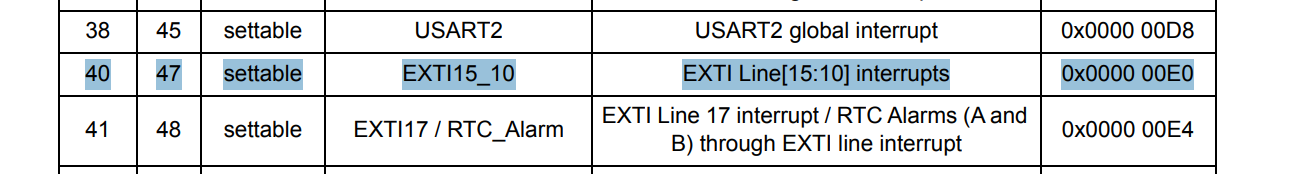
\includegraphics[width=0.8\linewidth]{imagens/IRQ.png}
    \caption{IRQ Vector Table}
    \label{fig:irq}
\end{figure}

Existe também a coluna \textit{Priority} que nesse caso tem o número 47, será explicado, após o \texttt{NVIC\_IPR}, o porquê.

\vspace{0.3cm}
\noindent\textbf{2. No Código-Fonte (A Mágica do CMSIS)}\\
Na prática do dia a dia, você não precisa ficar abrindo o PDF. O padrão CMSIS da ARM obriga a fabricante (ST) a criar um arquivo de cabeçalho mapeando todos esses números para você.
Se você investigar o arquivo principal do seu microcontrolador (por exemplo, \texttt{stm32f411xe.h}, que fica na pasta dos \texttt{Drivers/CMSIS}), você vai encontrar uma numeração (\texttt{enum}) gigante chamada \texttt{IRQn\_Type}. Ela mapeia exatamente a tabela do manual para a linguagem C:

\begin{lstlisting}[language=C]
typedef enum
{
/****** Cortex-M Processor Exceptions Numbers (Numeros negativos da ARM) ******/
  NonMaskableInt_IRQn         = -14,    /*!< 2 Non Maskable Interrupt         */
  HardFault_IRQn              = -13,    /*!< 3 Cortex-M Hard Fault Interrupt  */
  // ...
  
/****** STM32 specific Interrupt Numbers (A partir do zero) *******************/
  WWDG_IRQn                   = 0,      /*!< Window WatchDog Interrupt        */
  PVD_IRQn                    = 1,      /*!< PVD through EXTI Line detection  */
  // ...
  EXTI9_5_IRQn                = 23,     /*!< External Line[9:5] Interrupts    */
  // ...
  EXTI15_10_IRQn              = 40,     /*!< External Line[15:10] Interrupts  */
  // ...
} IRQn_Type;
\end{lstlisting}

É por isso que as funções da ARM funcionam tão bem. Quando você digita: \texttt{NVIC\_EnableIRQ(EXTI15\_10\_IRQn);}, o compilador C substitui silenciosamente a palavra \texttt{EXTI15\_10\_IRQn} pelo número 40. O NVIC usa esse número para ativar o bit exato no registrador de hardware que libera a interrupção.

\subsubsection*{A. Habilitando a Interrupção (NVIC\_ISER)}
O manual da ARM na página 220 define os registradores \texttt{NVIC\_ISER0} a \texttt{NVIC\_ISER7} (\textit{Interrupt Set-Enable Registers}) no endereço base \texttt{0xE000E100}. Como cada registrador tem 32 bits, eles controlam as interrupções em blocos de 32:
\begin{itemize}
    \item \texttt{ISER[0]}: IRQs 0 a 31
    \item \texttt{ISER[1]}: IRQs 32 a 63
\end{itemize}

Para a IRQ 40:
\begin{itemize}
    \item \textbf{Índice do Array:} $40 / 32 = 1$ (Usaremos o registrador \texttt{ISER[1]}).
    \item \textbf{Posição do Bit:} $40 \% 32 = 8$ (Usaremos o bit 8).
\end{itemize}

\subsubsection*{B. Configurando a Prioridade (NVIC\_IPR)}
Nas páginas 223 e 224, o manual descreve os registradores \texttt{NVIC\_IPR0} a \texttt{NVIC\_IPR59} (\textit{Interrupt Priority Registers}) a partir do endereço \texttt{0xE000E400}. Cada interrupção possui um campo de 8 bits (1 byte) para sua prioridade.

Isso significa que cada registrador de 32 bits abriga a prioridade de 4 IRQs diferentes. A STMicroelectronics (fabricante do STM32) implementa apenas os 4 bits mais significativos (bits 4 a 7) desse byte.

Para a IRQ 40:
\begin{itemize}
    \item \textbf{Índice do Array (Word de 32 bits):} $40 / 4 = 10$ (Usaremos o \texttt{IPR[10]}).
    \item \textbf{Deslocamento dentro da Word:} $(40 \% 4) \times 8 = 0$ (O byte da IRQ 40 ocupa os bits de 0 a 7 do \texttt{IPR[10]}).
\end{itemize}



\textbf{Ainda não sacou? A Estrutura do IPR}\\
O NVIC (controlador de interrupções) gerencia dezenas de interrupções diferentes (IRQ 0, IRQ 1, IRQ 2... até IRQ 239). O IRQ 0 pode ser um Timer, o IRQ 37 a UART1, e o IRQ 40 o \texttt{EXTI15\_10}.

Cada uma dessas interrupções precisa de um espaço na memória para guardar o seu ``nível de prioridade''. A ARM definiu por padrão que cada interrupção tem direito a exatos 8 bits (1 byte) para guardar sua prioridade.
A arquitetura Cortex-M é de 32 bits. Isso significa que cada ``gaveta'' (registrador) do IPR tem 32 bits de largura. Se você dividir os 32 bits de um registrador pelos 8 bits exigidos por interrupção, o resultado são 4 espaços.
Portanto, um único registrador IPR empacota a prioridade de 4 periféricos totalmente distintos. Veja como o array é preenchido sequencialmente:

\textbf{\texttt{IPR[0]} (Gaveta 0):}
\begin{itemize}
    \item \textbf{Byte 0} (bits 0 a 7): Guarda a prioridade da IRQ 0
    \item \textbf{Byte 1} (bits 8 a 15): Guarda a prioridade da IRQ 1
    \item \textbf{Byte 2} (bits 16 a 23): Guarda a prioridade da IRQ 2
    \item \textbf{Byte 3} (bits 24 a 31): Guarda a prioridade da IRQ 3
\end{itemize}

\textbf{\texttt{IPR[1]} (Gaveta 1):}
\begin{itemize}
    \item \textbf{Byte 0} (bits 0 a 7): Guarda a prioridade da IRQ 4
    \item \textbf{Byte 1} (bits 8 a 15): Guarda a prioridade da IRQ 5
    \item ... e assim por diante.
\end{itemize}

\textbf{A Matemática na Prática (O Exemplo do \texttt{EXTI15\_10})}\\
Quando você quer alterar a prioridade da interrupção do botão (\texttt{EXTI15\_10}), você precisa lembrar que ela corresponde à IRQ 40. Como o código (ou você, no Bare-Metal) descobre onde está a prioridade dela? Através de duas contas simples:
\begin{enumerate}
    \item \textbf{Em qual gaveta IPR ela está?} Divide-se o número da IRQ por 4.
    $40 / 4 = 10$. Logo, a configuração será escrita no registrador \texttt{IPR[10]}.
    \item \textbf{Em qual dos 4 espaços (bytes) dessa gaveta?} Pega-se o resto da divisão por 4.
    $40 \% 4 = 0$. O resto zero significa que ela ocupa o Byte 0 (o primeiro bloco, dos bits 0 a 7).
\end{enumerate}

Se fôssemos configurar a interrupção da UART1 (que é a IRQ 37):
\begin{itemize}
    \item $37 / 4 = 9 \rightarrow$ Está no registrador \texttt{IPR[9]}
    \item $37 \% 4 = 1 \rightarrow$ Está no Byte 1 (portanto, precisamos fazer um shift no valor da prioridade para escrevê-lo nos bits 8 a 15).
\end{itemize}

\textit{Resumindo:} O IPR é apenas um array de armazenamento onde as prioridades de todos os periféricos (EXTI, Timers, UART, I2C, etc.) são empacotadas de 4 em 4 para aproveitar todo o espaço dos registradores de 32 bits da CPU. O número 4 refere-se a esse empacotamento, e não ao comportamento do EXTI.

\subsubsection*{A Prioridade Pré-Definida (O Desempate do Hardware)}
Ao olhar para a Tabela de Vetores no Reference Manual da STMicroelectronics, notará uma coluna chamada \textit{Priority} que exibe números fixos crescentes (como o valor 47 para a linha \texttt{EXTI15\_10}). Mas se a prioridade é definida no código pelo programador (de 0 a 15), o que significa este número gravado no manual?

\textbf{1. A Matemática do Número 47}\\
O núcleo ARM Cortex-M possui as suas próprias exceções internas vitais de sistema operacional (como o Reset, HardFault, BusFault e o SysTick). Estas exceções ocupam o topo absoluto da cadeia alimentar de prioridades, assumindo os lugares do -3 ao 6.

Os periféricos externos criados pela ST (Timers, UART, EXTI) só começam a ser listados depois das exceções da ARM.
O primeiro IRQ da ST é o Watchdog (IRQ 0). Como as prioridades de 0 a 6 já estão ocupadas pela ARM, o IRQ 0 recebe a prioridade natural 7.
Seguindo essa lógica matemática impecável do hardware, o \texttt{EXTI15\_10}, que é o IRQ 40, recebe a prioridade natural de $40 + 7 = 47$.

\textbf{2. O Critério de Desempate (Hardware Tie-Breaker)}\\
Esse número é a Prioridade Fixa de Hardware. Ele não pode ser alterado, pois é definido pelo local onde os fios de silício estão fisicamente ligados dentro do microcontrolador. Ele serve para um único propósito: \textbf{desempatar colisões}.

Imagine a seguinte situação:
Através do código C (\texttt{HAL\_NVIC\_SetPriority}), definiu a interrupção da UART1 e a interrupção do botão (\texttt{EXTI15\_10}) com a mesma prioridade lógica (ex: Nível 5). Por uma coincidência estatística, um dado chega na UART e o utilizador prime o botão no exato mesmo microssegundo. As duas flags levantam ao mesmo tempo. Quem é que a CPU atende primeiro?

Neste cenário de colisão, o NVIC ignora o software e consulta a Prioridade Fixa de Hardware:
\begin{itemize}
    \item A UART1 (IRQ 37) tem a prioridade física \textbf{44}.
    \item O EXTI15\_10 (IRQ 40) tem a prioridade física \textbf{47}.
\end{itemize}
O número menor indica sempre a prioridade mais alta. Logo, o NVIC encaminha a CPU para atender a UART1 primeiro, e o botão fica na fila de espera.

\textit{Nota importante:} A prioridade de software configurada pelo programador tem sempre prevalência. Se der o Nível 1 ao botão e o Nível 5 à UART, o botão irá sempre interromper a UART, independentemente de ter o número físico 47. O hardware só usa este valor fixo quando há um empate estrito.

\subsubsection*{Código C (Nível Bare Metal Absoluto)}
Aqui está como você escreve isso no seu \texttt{main.c}, substituindo as chamadas do CMSIS. Defini os endereços usando pointers explícitos.

\begin{lstlisting}[language=C]
/* ===================================================================== */
/* DEFINICOES DO NVIC (Extraidas do ARM Cortex-M4 Generic User Guide)    */
/* ===================================================================== */

/* Enderecos base dos registradores do NVIC */
#define NVIC_ISER_BASE  0xE000E100UL
#define NVIC_IPR_BASE   0xE000E400UL

/* Cast dos enderecos para ponteiros de arrays volateis de 32 bits */
#define NVIC_ISER  ((volatile uint32_t *)NVIC_ISER_BASE)
#define NVIC_IPR   ((volatile uint32_t *)NVIC_IPR_BASE)

/* Numero da Interrupcao (Especifico do microcontrolador) */
#define EXTI15_10_IRQn  40


/* ===================================================================== */
/* FUNCAO DE INICIALIZACAO (Substitui NVIC_SetPriority e EnableIRQ)      */
/* ===================================================================== */
static void nvicInitDirect(void)
{
  /* 1. NVIC: Configurar a Prioridade (Equivalente a NVIC_SetPriority) */
  /* Limpamos o byte 0 (bits 0 a 7) do IPR[10] para definir prioridade 0. */
  /* Mascara 0xFF (11111111) movida 0 posicoes. */
  NVIC_IPR[10] &= ~(0xFFUL << 0);
  
  /* Se voce quisesse prioridade 2, por exemplo, o codigo seria:
   * NVIC_IPR[10] &= ~(0xFFUL << 0);
   * NVIC_IPR[10] |=  (2UL << 4); // Shift de 4 porque so os MSB importam no STM32
   */

  /* 2. NVIC: Habilitar a Interrupcao (Equivalente a NVIC_EnableIRQ) */
  /* O registrador ISER[1] cobre da IRQ 32 a 63. */
  /* A IRQ 40 corresponde ao bit 8 (40 - 32 = 8). */
  /* Como e um registrador Set-Enable, nao precisamos ler antes (nao usa |=), apenas escrever o bit. */
  NVIC_ISER[1] = (1UL << 8); 
}
\end{lstlisting}

\subsubsection*{3. O Arquivo Startup e a Tabela de Vetores (startup\_stm32f411xe.s)}
O \texttt{Reset\_Handler} e a Tabela de Vetores não são gerados pelo CubeMX em C. Eles são escritos em linguagem Assembly dentro de um arquivo \texttt{.s} que o compilador anexa ao seu projeto. Se abrirmos esse arquivo, veremos como ele mapeia os endereços das interrupções:

\begin{lstlisting}[language=C]
/* Estrutura simplificada do startup_stm32f4xxxx.s */

/* A TABELA DE VETORES (Array de ponteiros gravado na Flash) */
.section .isr_vector,``a'',%progbits
  .word  _estack                  /* 0x00000000: Topo da RAM (Stack Pointer) */
  .word  Reset_Handler            /* 0x00000004: Ponteiro para o Reset_Handler */
  .word  NMI_Handler              /* 0x00000008: Non Maskable Interrupt */
  .word  HardFault_Handler        /* 0x0000000C: Falha Critica de Hardware */
  /* ... dezenas de ponteiros internos da ARM ... */
  .word  EXTI0_IRQHandler         /* Interrupcao Externa da Linha 0 */
  /* ... */
  .word  EXTI15_10_IRQHandler     /* Interrupcao Externa das Linhas 10 a 15 */
\end{lstlisting}

Quando o NVIC detecta a borda de descida no botão, ele pega o número da interrupção, calcula a posição dela nessa tabela de vetores, lê o endereço que está escrito ali (\texttt{.word EXTI15\_10\_IRQHandler}) e manda a CPU pular para lá.

\textbf{O Truque do \texttt{\_\_weak} (E por que o sistema trava)}\\
No mesmo arquivo Assembly, logo abaixo da tabela, os programadores da ST definem todas as funções de interrupção (como \texttt{EXTI15\_10\_IRQHandler}) usando a diretiva \texttt{weak} e apontando para um ``buraco negro'' chamado \texttt{Default\_Handler}.

\begin{lstlisting}[language=C]
/* Definicao de fallback (seguranca) */
.weak EXTI15_10_IRQHandler
.thumb_set EXTI15_10_IRQHandler, Default_Handler

/* O Buraco Negro */
Default_Handler:
Infinite_Loop:
  b Infinite_Loop /* ``Branch'' (pula) para si mesmo infinitamente */
\end{lstlisting}

\textbf{Como isso impacta seu código C:}\\
A diretiva \texttt{.weak} (fraca) diz ao compilador (Linker): ``Se o usuário não criar uma função chamada \texttt{EXTI15\_10\_IRQHandler} no arquivo \texttt{.c} dele, use o \texttt{Default\_Handler} no lugar''.
É por isso que, se você habilitar a interrupção no hardware (IMR e NVIC), mas esquecer de escrever a função \texttt{EXTI15\_10\_IRQHandler(void)} no seu \texttt{main.c}, o microcontrolador não vai dar erro de compilação. Mas, quando você apertar o botão, o NVIC vai redirecionar a CPU para o \texttt{Default\_Handler}, que é um loop infinito (\texttt{while(1)} vazio em Assembly). O seu chip vai travar completamente e a única saída será apertar o botão de Reset.

Quando você escreve a função no seu \texttt{main.c}, o Linker substitui a referência \texttt{weak}, e o ponteiro na Tabela de Vetores passa a apontar para o seu código de fato.

\textbf{A fórmula universal para encontrar qualquer interrupção dentro do array IPR é:}
\begin{itemize}
    \item \textbf{Índice do Registrador:} IRQ / 4
    \item \textbf{Deslocamento base (Shift):} (IRQ \% 4) * 8
\end{itemize}

Vamos usar como exemplo prático a IRQ 38 (que no STM32F4 corresponde ao periférico SPI3).
\begin{itemize}
    \item $38 / 4 = 9$. Logo, vamos alterar o registrador \texttt{IPR[9]}.
    \item $38 \% 4 = 2$. O resto 2 significa que ela ocupa o Byte 2 (o terceiro espaço).
    \item $2 \times 8 = 16$. Nosso deslocamento base é de 16 casas para a esquerda.
\end{itemize}

\textbf{O ``Pulo do Gato'' da STMicroelectronics}\\
Antes do código, um detalhe crucial de hardware: embora o manual da ARM reserve 8 bits (1 byte) inteiros para a prioridade, fabricantes de silício podem escolher implementar menos bits para economizar transistores.

A STMicroelectronics escolheu implementar apenas \textbf{4 bits por interrupção} no STM32F4. Pelo padrão da ARM, esses bits implementados devem ser sempre os Mais Significativos (MSB) do byte. Portanto, dentro daquele espaço de 8 bits, apenas os 4 bits superiores (bits 4, 5, 6 e 7) funcionam de verdade. Os 4 inferiores (0 a 3) são ignorados pelo hardware.
Isso significa que o valor da nossa prioridade precisa sofrer um \textit{shift} adicional de 4 casas em cima do deslocamento base.

\textbf{O Código (Bare Metal)}
\begin{lstlisting}[language=C]
/* ===================================================================== */
/* EXEMPLO PRATICO: Configurando prioridade de uma IRQ no Byte 2         */
/* ===================================================================== */

/* Usando a IRQ 38 (ex: SPI3) */
/* Indice: 38 / 4 = 9  -> IPR[9] */
/* Shift base: (38 % 4) * 8 = 16 */

/* Passo 1: Limpar o campo de prioridade antigo (Read-Modify-Write) */
/* A mascara 0xFF (11111111 em binario) cobre 1 byte inteiro. */
/* Deslocamos essa mascara 16 casas para a esquerda, caindo exatamente no Byte 2. */
/* O operador ~ inverte a mascara (zeros onde queremos apagar) e o & aplica. */
NVIC_IPR[9] &= ~(0xFFUL << 16);

/* Passo 2: Escrever a nova prioridade (exemplo: Prioridade 5) */
/* A ST usa apenas os 4 bits mais significativos (MSB) do byte. */
/* Portanto, o shift final e: Shift Base (16) + Deslocamento ST (4) = 20. */
/* Valor 5 (0101 em binario) e deslocado 20 casas para a esquerda. */
NVIC_IPR[9] |= (5UL << (16 + 4));
\end{lstlisting}

Com essa lógica, você consegue mapear absolutamente qualquer interrupção (de 0 a 240) manipulando bits manualmente, sem depender de nenhuma função pronta da ST ou da ARM. Se a IRQ caísse no Byte 3 (ex: IRQ 39), o \textit{shift} base seria 24, e o shift da prioridade seria 28 (24 + 4).

% ==========================================
% ANEXO 6: BOOT0, BOOT1 e NRST (RESET)
% ==========================================
\subsection*{Anexo 6: BOOT0, BOOT1 e NRST (RESET)}
\label{anexo:6}
\addcontentsline{toc}{subsection}{Anexo 6: BOOT0, BOOT1 e NRST (RESET)}



\subsubsection*{1. O mistério do BOOT0 e BOOT1}
No microcontrolador (o chip preto soldado na placa), o BOOT0 é sim um pino físico.
O que acontece é que a fabricante da sua placa de desenvolvimento colocou um botão tátil chamado BOOT0 para facilitar a sua vida. Esse botão está ligado diretamente ao pino BOOT0 do chip.
\begin{itemize}
    \item O pino possui um resistor de pull-down (puxando para GND).
    \item Quando você não aperta o botão, o pino lê 0.
    \item Quando você aperta o botão, ele conecta o pino ao 3.3V, e o chip lê 1.
\end{itemize}

\textbf{E o BOOT1?}\\
No STM32F411, para economizar pinos no encapsulamento, o BOOT1 não tem um pino dedicado exclusivo. Ele é ``multiplexado''. O chip lê o estado do pino normal de I/O \texttt{PB2} no exato milissegundo em que é ligado para saber o valor do BOOT1.

A combinação desses dois no momento em que a energia entra no chip (ou após um reset) define a tal região de \textit{Aliasing} (Espelhamento) que discutimos antes:
\begin{itemize}
    \item \textbf{BOOT0 = 0:} O chip espelha a \textit{Main Flash memory} (seu código C compilado) para o endereço \texttt{0x0000 0000} e roda o seu programa.
    \item \textbf{BOOT0 = 1 e BOOT1 (PB2) = 0:} O chip espelha a \textit{System memory}. Essa é uma memória ROM de fábrica da ST que contém um Bootloader. É ele que permite que você grave o chip via cabo USB (DFU) ou UART usando o STM32CubeProgrammer, sem precisar de um gravador ST-Link externo.
\end{itemize}

\subsubsection*{2. O Pino RESET vs. O Botão RESET}
A sua dedução está 100\% correta. Fazem exatamente a mesma coisa, porque são fisicamente a mesma coisa.
No datasheet, você vai ver esse pino nomeado como \textbf{NRST} (\textit{Negative Reset}). O ``N'' significa que ele usa lógica invertida (Ativo em Baixo).

O chip possui um circuito interno (ou um resistor externo na placa) que mantém o pino NRST constantemente alimentado com 3.3V (ALTO). Enquanto tiver tensão ali, o processador trabalha feliz. Se a tensão nesse pino cair para 0V (BAIXO), o processador trava imediatamente. Quando a tensão volta para 3.3V, ele recomeça o programa da linha zero.

O botão de RESET da sua placa é literalmente uma chavinha mecânica com um lado soldado no pino NRST do chip e o outro lado soldado no GND (Terra/0V). Você aperta o botão $\rightarrow$ cria um curto-circuito com o GND $\rightarrow$ a tensão do pino NRST cai para zero $\rightarrow$ o chip reseta.

\subsubsection*{Resumo}
\textbf{Atenção à Placa vs. Datasheet:} Nos esquemáticos e datasheets do STM32, o boot é definido pelo estado dos pinos BOOT0 e BOOT1 (frequentemente mapeado no pino PB2). Em placas de desenvolvimento comerciais, o pino BOOT0 é roteado para um botão físico para facilitar a entrada no modo Bootloader (DFU) via USB. Da mesma forma, o botão de Reset da placa é apenas um interruptor tátil conectado entre o pino físico NRST (\textit{Active-Low Reset}) e o Terra (GND).

\begin{table}[H]
    \centering
    \resizebox{\textwidth}{!}{%
    \begin{tabular}{ccclp{8cm}}
    \toprule
    \textbf{BOOT0} & \textbf{BOOT1 (PB2)} & \textbf{Memória Selecionada} & \textbf{Endereço Físico} & \textbf{Descrição da Memória} \\
    \midrule
    0 & X (N/A) & \textbf{Main Flash Memory} & \texttt{0x08000000} & É a memória ROM onde o seu código C (\texttt{main.bin}) é permanentemente gravado. É a configuração padrão. \\
    \midrule
    1 & 0 & \textbf{System Memory} & \texttt{0x1FFF0000} & Memória ROM protegida gravada de fábrica. Contém o Bootloader original para gravação via USB (DFU) ou UART. \\
    \midrule
    1 & 1 & \textbf{SRAM} & \texttt{0x20000000} & RAM principal. Usado quase exclusivamente para debug avançado, rodando código na RAM para poupar a Flash. \\
    \bottomrule
    \end{tabular}}
\end{table}

% ==========================================
% ANEXO 7: Arquitetura do STM32
% ==========================================
\subsection*{Anexo 7: Arquitetura do STM32}
\label{anexo:7}
\addcontentsline{toc}{subsection}{Anexo 7: Arquitetura do STM32}

\begin{figure}[H]
    \centering
    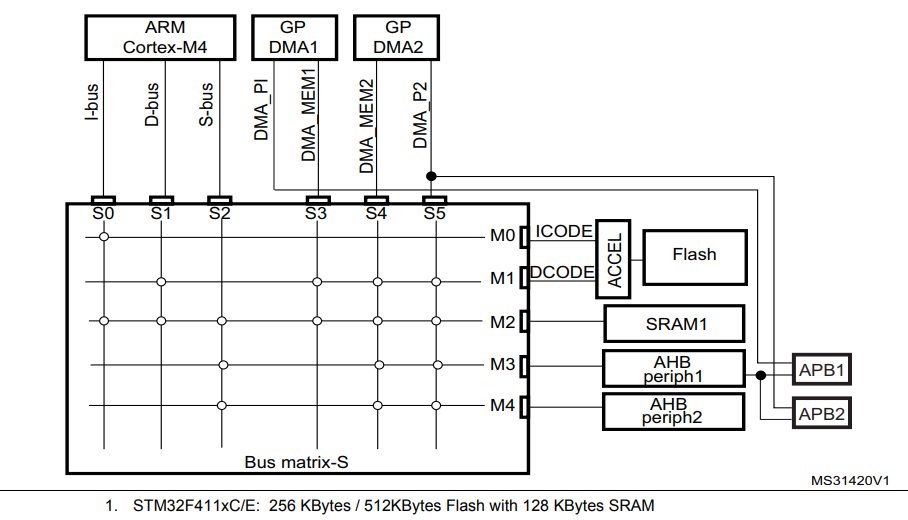
\includegraphics[width=0.8\linewidth]{imagens/Architecture.png}
    \caption{System Architecture}
    \label{fig:architecture}
\end{figure}

O microcontrolador STM32 não é um bloco monolítico. Ele é um sistema híbrido complexo, como um carro onde o motor é feito por uma empresa e o resto do chassi por outra.
\begin{itemize}
    \item \textbf{O Cérebro (ARM Cortex-M):} É a CPU propriamente dita. A empresa ARM projeta o núcleo (o ``motor''), que inclui a unidade de processamento, o controlador de interrupções (NVIC) e o Timer do sistema (SysTick). A STMicroelectronics apenas licencia esse design.
    \item \textbf{O Corpo (ST Microelectronics):} A ST pega esse núcleo da ARM e constrói todo o ``silício'' ao redor dele: as memórias Flash e RAM, os GPIOs, as UARTs, Timers e os barramentos que ligam tudo.
\end{itemize}

\subsubsection*{A Matrix de Barramentos (Bus Matrix)}
Como o cérebro fala com o corpo? Através de um complexo sistema de rodovias digitais chamado \textbf{Bus Matrix}.
Quando a CPU quer acender um LED, ela não tem um fio direto para o pino. Ela gera um endereço de memória (ex: \texttt{0x40020014} para o ODR do GPIOA) e joga no barramento. A Bus Matrix age como um guarda de trânsito, identificando que esse endereço pertence ao periférico GPIOA e roteando os dados para a ``rodovia'' correta (o barramento AHB1) até chegar ao destino.

\subsubsection*{O Mapa de Memória (Memory Map)}
Sendo um processador de 32 bits, o STM32 consegue endereçar $2^{32}$ posições de memória. Isso cria um ``espaço virtual'' linear gigante de 4 Gigabytes (do endereço \texttt{0x0000 0000} até \texttt{0xFFFF FFFF}).



O truque é: o chip não tem 4GB de memória real. A grande maioria desse espaço é um vazio. A STMicroelectronics e a ARM ``mapeiam'' (colam) as coisas físicas (Flash, RAM, Periféricos) em blocos específicos desse espaço de 4GB.

\begin{verbatim}
MAPA DE MEMÓRIA STM32 (Espaço de Endereçamento Linear de 4GB)
===========================================================

Endereço Final (Topo) -> 0xFFFF FFFF
+---------------------------------------------------------+
|                                                         |
|   AREA RESERVADA PELA ARM (Cortex-M Internal PPB)       |
|   - Onde vivem o NVIC e o SysTick                       |
|   - Início: 0xE000 0000                                 |
+---------------------------------------------------------+
|                                                         |
|                     (Vazio / Reservado)                 |
|                                                         |
+---------------------------------------------------------+ <- 0x5FFF FFFF
|                                                         |
|   AREA DE PERIFÉRICOS DA ST (Peripheral Region)         |
|   - AHB (GPIOs): Início 0x4002 0000                     |
|   - APB2 (Rápido): Início 0x4001 0000                   |
|   - APB1 (Lento): Início 0x4000 0000                    |
+---------------------------------------------------------+ <- 0x4000 0000
|                                                         |
|                     (Vazio / Reservado)                 |
|                                                         |
+---------------------------------------------------------+ <- 0x3FFF FFFF
|                                                         |
|   AREA DA MEMÓRIA RAM (SRAM Region)                     |
|   - Onde vivem suas variáveis, Stack e Heap             |
|   - Início: 0x2000 0000                                 |
+---------------------------------------------------------+ <- 0x2000 0000
|                                                         |
|                     (Vazio / Reservado)                 |
|                                                         |
+---------------------------------------------------------+ <- 0x0810 0000 (aprox)
|   AREA DE CÓDIGO (Flash Memory Real)                    |
|   - Início físico: 0x0800 0000                          |
+---------------------------------------------------------+
|   AREA DE BOOT (System Memory / Bootloader ST)          |
|   - Início: 0x1FFF xxxx (Varia com o chip)              |
+---------------------------------------------------------+
|   AREA DE ESPELHAMENTO (Aliasing)                       |
|   - O endereço 0x0000 0000 reflete uma das memórias     |
|     acima dependendo dos pinos BOOT.                    |    (End. Base)
+---------------------------------------------------------+ <- 0x0000 0000
\end{verbatim}

Vamos detalhar as quatro regiões principais mostradas:
\begin{enumerate}
    \item \textbf{Code Region (Onde seu programa vive):} Começa no endereço \texttt{0x0000 0000}. Como discutimos na seção de Boot, este início é um ``espelho'' (alias). A memória Flash real, onde seu código binário (\texttt{.bin}) é gravado, começa fisicamente em \texttt{0x0800 0000}. A System Memory (o Bootloader de fábrica da ST) fica escondida em uma área reservada por volta de \texttt{0x1FFF xxxx}.
    \item \textbf{SRAM Region (Sua bancada de trabalho):} Começa em \texttt{0x2000 0000}. É a memória volátil (RAM). Todas as suas variáveis globais, o Stack (pilha de funções) e o Heap (alocação dinâmica \texttt{malloc}) vivem aqui. Quando você cria uma variável \texttt{int contador = 0;}, o compilador reserva 4 bytes físicos dentro dessa região.
    \item \textbf{Peripheral Region (O território da ST):} Começa em \texttt{0x4000 0000}. Este é o bloco mais importante para nós. A ST mapeia todos os registradores de controle aqui. Eles são divididos pelos barramentos de velocidade:
    \begin{itemize}
        \item \textbf{APB1 (Lento):} Começa na base \texttt{0x4000 0000} (Timers 2-5, UART2, I2C1).
        \item \textbf{APB2 (Rápido):} Começa em \texttt{0x4001 0000} (TIM1, ADC1, SPI1, SYSCFG).
        \item \textbf{AHB (Expresso):} Começa em \texttt{0x4002 0000} (Todos os GPIOs, RCC, DMA).
    \end{itemize}
    \textit{Na prática:} Quando você escreve \texttt{GPIOA->MODER = ...} no código, o ponteiro \texttt{GPIOA} nada mais é do que um \texttt{\#define} para o endereço fixo \texttt{0x40020000}. A CPU está literalmente escrevendo naquele local físico.
    \item \textbf{Cortex-M Internal PPB (O território da ARM):} Fica lá no topo, começando em \texttt{0xE000 0000}. PPB significa \textit{Private Peripheral Bus}. Aqui vivem os componentes que vêm ``dentro da caixa'' do processador da ARM, não importando se o chip é um STM32, um NXP ou um Texas Instruments. É aqui que estão os registradores do NVIC (\texttt{ISER}, \texttt{IPR}) e do SysTick Timer. Por isso a documentação deles fica em um manual separado da ARM, e não no manual principal da ST.
\end{enumerate}

% ==========================================
% ANEXO 8: RCC (Extras)
% ==========================================
\subsection*{Anexo 8: RCC (Extras)}
\label{anexo:8}
\addcontentsline{toc}{subsection}{Anexo 8: RCC (Extras)}

Nós cobrimos a parte principal do dia a dia: a habilitação de energia para os periféricos (os registradores \texttt{ENR}) e a seleção da fonte principal do relógio (HSI, HSE e PLL). No entanto, como a própria sigla diz (\textit{Reset and Clock Control}), faltou falarmos da letra ``R'' e de alguns mecanismos de segurança que são essenciais, especialmente em contextos de aviônica e sistemas críticos.

Aqui estão as 3 peças do RCC que ainda não abordamos detalhadamente:

\subsubsection*{1. O Reset Individual de Periféricos (RSTR)}
Até agora, usamos registradores como o \texttt{APB1ENR} para ligar o clock de um periférico. Mas o RCC também possui os registradores de Reset (ex: \texttt{AHB1RSTR}, \texttt{APB1RSTR}, \texttt{APB2RSTR}).
\begin{itemize}
    \item \textbf{Para que serve:} Imagine que o seu barramento I2C travou no meio do voo porque o sensor mandou um sinal corrompido. Você não pode dar um reboot no microcontrolador inteiro (e desligar o motor).
    \item \textbf{Como funciona:} Você vai no registrador \texttt{RCC->APB1RSTR}, levanta o bit correspondente ao I2C1 e depois abaixa. O hardware do STM32 corta a energia e reinicia apenas o circuito de silício do I2C, limpando qualquer travamento, enquanto o resto da CPU e o PWM continuam rodando intactos.
\end{itemize}
\textit{Na HAL, isso é feito pelas funções \texttt{\_\_HAL\_RCC\_I2C1\_FORCE\_RESET()} e \texttt{\_\_HAL\_RCC\_I2C1\\\_RELEASE\_RESET()}.}

\subsubsection*{2. Os Divisores de Barramento (CFGR)}
Nós mencionamos que o APB1 é o ``barramento lento'' e o APB2 é o ``barramento rápido''. Mas quem define isso? É o \textit{Clock Configuration Register} (\texttt{CFGR}) dentro do RCC.
A CPU pode estar rodando a 100 MHz (SYSCLK). O registrador CFGR possui bits chamados de \textit{Prescalers} (\texttt{HPRE} para o AHB, \texttt{PPRE1} para o APB1 e \texttt{PPRE2} para o APB2).
É lá que você (ou a função \texttt{SystemClock\_Config} gerada pelo CubeMX) diz ao hardware: ``Pegue os 100 MHz da CPU e divida por 2 antes de entregar para o APB1''. Sem configurar os divisores no CFGR, os timers e a UART receberiam frequências erradas e o cálculo do Baud Rate daria errado.

\subsubsection*{3. O Sistema de Segurança do Clock (CSS - Clock Security System)}
Em hardware profissional, se você usa um cristal de quartzo externo (HSE) para ter precisão, existe o risco físico de a solda trincar devido à vibração de um foguete ou drone, fazendo o cristal parar de bater. Se o clock parar, a CPU congela e o veículo cai.



O RCC possui um bit chamado \texttt{CSSON} (\textit{Clock Security System Enable}) no registrador de controle (\texttt{CR}).
\begin{itemize}
    \item Se você ativar esse bit, um circuito de hardware independente fica monitorando o cristal externo.
    \item Se o cristal quebrar e o pulso falhar, o hardware automaticamente desliga o HSE, liga o oscilador interno (HSI) para a CPU não morrer, e dispara uma Interrupção Não Mascarável (NMI) gravíssima no NVIC, para que o seu código C possa executar um procedimento de emergência.
\end{itemize}

Esses três pontos fecham 100\% das responsabilidades do bloco RCC.

% ==========================================
% ANEXO 9: RTC (Real-Time Clock)
% ==========================================
\subsection*{Anexo 9: RTC (Real-Time Clock)}
\label{anexo:9}
\addcontentsline{toc}{subsection}{Anexo 9: RTC (Real-Time Clock)}

Enquanto os Timers convencionais (como o TIM2 ou TIM3) são cronômetros esportivos que medem intervalos de tempo relativos e zeram quando o chip perde energia, o RTC é o seu relógio de pulso com calendário. Ele sabe que dia, mês, ano, hora, minuto e segundo exatos estamos vivendo.

A maior força do RTC no STM32 é o \textit{Backup Domain} (Domínio de Backup). O hardware do RTC fica isolado do resto do processador. Se a energia principal da placa for cortada (ou o foguete der um reset no ar), o RTC puxa energia automaticamente de uma bateria tipo ``moeda'' (ligada ao pino VBAT) e continua contando o tempo sem perder um único milissegundo.



\subsubsection*{1. A Matemática do Relógio (O Cristal LSE)}
Para economizar a bateria externa, o RTC não usa o relógio principal veloz do sistema. Ele exige a soldagem de um cristal de quartzo cilíndrico dedicado, chamado LSE (\textit{Low-Speed External}).

A frequência mundial padrão para cristais de relógio é 32.768 kHz. Isso não é um número aleatório. É exatamente $2^{15}$. O hardware do RTC possui dois divisores de frequência (Prescalers, o Assíncrono e o Síncrono) que dividem essa oscilação perfeitamente para gerar o pulso de 1 Hz. A fórmula que o silício executa é:
\[ f_{RTC} = \frac{32768}{(PREDIV\_A + 1) \times (PREDIV\_S + 1)} = 1 \text{ Hz} \]
Na prática (e no CubeMX), o Prescaler Assíncrono é setado para 127 e o Síncrono para 255. A divisão perfeita resulta em 1 segundo cravado.

\subsubsection*{2. O Formato BCD (Binary-Coded Decimal)}
Diferente do resto do chip, o RTC não guarda o número ``26'' como \texttt{0x1A} (o binário real). Ele guarda a dezena e a unidade separadamente em ``pacotes'' de 4 bits, o chamado BCD.
\begin{itemize}
    \item Para o ano 26: O dígito 2 em 4 bits (\texttt{0010}) e o dígito 6 em 4 bits (\texttt{0110}).
    \item Valor no registrador: \texttt{0010 0110} (Lido no código hexadecimal como \texttt{0x26}).
\end{itemize}

\subsubsection*{3. RTC com HAL (A Armadilha da Sombra)}
O CubeMX gera o código de inicialização \texttt{MX\_RTC\_Init()} configurando o calendário. O mais importante é como ler esses dados no seu \texttt{while(1)}.

\textbf{Regra de Ouro da HAL no RTC:} O hardware do RTC usa ``Registradores Sombra'' (\textit{Shadow Registers}). Quando você lê a Hora, o hardware congela a Data nos bastidores para garantir que você não leia a data errada caso o dia vire no exato milissegundo da leitura.
Por isso, você é \textbf{obrigado a ler a Data logo após a Hora}, mesmo que não vá usá-la. Se ler só a Hora, o hardware trava os registradores esperando você ler a Data, e o seu relógio ``congela'' na tela.

\begin{lstlisting}[language=C]
/* Variaveis para guardar os dados */
RTC_TimeTypeDef sTime = {0};
RTC_DateTypeDef sDate = {0};

/* Dentro do seu while(1) */

/* 1. LER A HORA PRIMEIRO */
/* Usamos RTC_FORMAT_BIN para a HAL ja converter o BCD para decimal normal (int) */
HAL_RTC_GetTime(&hrtc, &sTime, RTC_FORMAT_BIN);

/* 2. LER A DATA LOGO EM SEGUIDA (Obrigatorio para destravar o hardware!) */
HAL_RTC_GetDate(&hrtc, &sDate, RTC_FORMAT_BIN);

/* Agora as variaveis estao limpas e prontas para uso */
printf("Data: %02d/%02d/20%02d\r\n", sDate.Date, sDate.Month, sDate.Year);
printf("Hora: %02d:%02d:%02d\r\n", sTime.Hours, sTime.Minutes, sTime.Seconds);
\end{lstlisting}

\subsubsection*{4. RTC no ``Bare-Metal'' (Abrindo o Cofre)}
Configurar o RTC direto nos registradores ensina muito sobre a segurança arquitetural do ARM Cortex. O RTC é tratado como um ``cofre''. Você não pode simplesmente escrever a hora nele, pois ruídos elétricos acidentais poderiam corromper o calendário.

O processo exige três chaves de segurança:
\begin{enumerate}
    \item Ligar a energia do Backup Domain (Registrador \texttt{PWR->CR}).
    \item Ligar o cristal LSE e esperar ele estabilizar (Registrador \texttt{RCC->BDCR}).
    \item Entrar no Modo de Inicialização (INIT) (Registrador \texttt{RTC->ISR}). Só neste modo o relógio para de bater e permite que você altere os ponteiros.
\end{enumerate}

\begin{lstlisting}[language=C]
/* ========================================================== */
/* 1. DESTRAVANDO O COFRE (Backup Domain)                     */
/* ========================================================== */
RCC->APB1ENR |= (1UL << 28);      // Liga o clock do controlador de Energia (PWR)
PWR->CR |= (1UL << 8);            // DBP: Abre a fechadura do cofre

/* ========================================================== */
/* 2. LIGANDO O CRISTAL DE RELOGIO (LSE)                      */
/* ========================================================== */
RCC->BDCR |= (1UL << 0);          // LSEON: Liga o cristal externo de 32.768 kHz
while (!(RCC->BDCR & (1UL << 1)));// Espera o bit LSERDY ir a 1 (Cristal estabilizou)

/* Define o LSE como fonte do RTC e liga o RTC */
RCC->BDCR |= (1UL << 8);          // RTCSEL: Seleciona LSE (01)
RCC->BDCR |= (1UL << 15);         // RTCEN: Liga o motor do RTC

/* ========================================================== */
/* 3. MODO INIT E CONFIGURACAO DE HORA (Ex: 14:30:00)         */
/* ========================================================== */
/* Escreve as chaves magicas para destravar os registradores do RTC */
RTC->WPR = 0xCA; 
RTC->WPR = 0x53;

RTC->ISR |= (1UL << 7);           // INIT: Pede para entrar no modo de configuracao
while (!(RTC->ISR & (1UL << 6))); // Espera a flag INITF confirmar a entrada

/* Configura os Prescalers (127 Assincrono, 255 Sincrono) */
RTC->PRER = (127UL << 16) | (255UL);

/* Ajusta a Hora no Registrador TR (Time Register) usando formato BCD */
/* Exemplo: 14h 30m 00s */
RTC->TR = (1UL << 20) | (4UL << 16) |  // Dezenas(1) e Unidades(4) da Hora
          (3UL << 12) | (0UL << 8)  |  // Dezenas(3) e Unidades(0) dos Minutos
          (0UL << 4)  | (0UL << 0);    // Dezenas(0) e Unidades(0) dos Segundos

RTC->ISR &= ~(1UL << 7);          // Sai do modo INIT (O relogio volta a bater com nova hora)

/* Tranca o cofre novamente */
RTC->WPR = 0xFF;                  // Escreve chave invalida para travar
\end{lstlisting}

\textit{Para ler no Bare-Metal:} Basta ler os registradores \texttt{RTC->TR} (Tempo) e \texttt{RTC->DR} (Data) e fazer o ``shift'' invertido e a matemática para transformar o BCD em formato decimal legível no seu display. Lembre-se que o hardware atualiza esses registradores sozinho a cada segundo.

% ==========================================
% ANEXO 10: Stack/Heap Sizes
% ==========================================
\subsection*{Anexo 10: Stack/Heap Sizes}
\label{anexo:10}
\addcontentsline{toc}{subsection}{Anexo 10: Stack/Heap Sizes}

Manter esses valores mínimos na configuração padrão é a receita número um para travamentos misteriosos (\textit{Hard Faults}) quando o seu projeto começar a ganhar corpo.

Com 128 KB de RAM no STM32F411, você é praticamente um ``milionário'' em termos de memória para sistemas embarcados. Deixar os valores padrão de \texttt{0x200} (512 Bytes) e \texttt{0x400} (1024 Bytes) é ser excessivamente econômico sem necessidade.



\subsubsection*{1. O Stack (A Pilha de Execução) - Onde o perigo mora}
O Stack é a memória de uso ultrarrápido gerenciada automaticamente pelo compilador. Ele guarda:
\begin{itemize}
    \item Variáveis locais (criadas dentro das funções).
    \item O endereço de retorno das funções (para a CPU saber para onde voltar quando a função acabar).
    \item O contexto dos registradores quando ocorre uma interrupção.
\end{itemize}

\textbf{O Problema do Padrão (\texttt{0x400} = 1 KB):}\\
Se você tiver um Stack de 1 KB e, dentro de uma função que lê um sensor, você declarar \texttt{uint8\_t buffer\_sd[2048];}, o seu código vai compilar sem erros. Mas no instante em que essa função for chamada na placa, a variável vai atropelar o limite do Stack e invadir outras memórias. O processador capota na hora.
Outro vilão é a função \texttt{printf()}. Quando você manda imprimir um número com vírgula (\texttt{float \%f}), a biblioteca C padrão consome uma quantidade absurda de Stack para fazer a conversão de texto.

\textbf{Recomendação:} Suba o \textit{Minimum Stack Size} para pelo menos \textbf{\texttt{0x1000} (4 KB)} ou \textbf{\texttt{0x2000} (8 KB)}. Custa quase nada dos seus 128 KB e garante que suas funções pesadas e interrupções rodem com folga.

\subsubsection*{2. O Heap (A Pilha Dinâmica) - A regra da aviônica}
O Heap é o oposto. É um espaço de memória reservado exclusivamente para alocação dinâmica. É a área que você usa quando chama a função \texttt{malloc()} no C para criar arrays cujo tamanho você só descobre durante a execução do programa.

Na engenharia aeroespacial e no desenvolvimento de sistemas críticos, existe uma regra de ouro implacável: \textbf{Nunca se usa alocação dinâmica (\texttt{malloc}) em voo}. O motivo é a ``fragmentação de memória''. Se você ficar alocando e liberando blocos de memória, o Heap vira um queijo suíço. Em algum momento crítico, o código vai pedir memória, o sistema não vai achar um bloco contínuo vazio, o \texttt{malloc} vai retornar \texttt{NULL}, e o sistema trava.

\textbf{Recomendação:} A menos que você vá usar o FreeRTOS (que precisa de Heap para criar tarefas), você não deve usar \texttt{malloc()} nos seus códigos de controle. Portanto, o \textit{Minimum Heap Size} pode ficar tranquilo no padrão de \textbf{\texttt{0x200}} (ou até \texttt{0x000}), já que ele será praticamente inútil na sua arquitetura Bare-Metal/HAL.

\end{document}